% Created 2021-10-02 Sat 15:44
% Intended LaTeX compiler: pdflatex
\documentclass{scrartcl}
\usepackage[utf8]{inputenc}
\usepackage[T1]{fontenc}
\usepackage{fontspec}
\usepackage{graphicx}
\usepackage{grffile}
\usepackage{longtable}
\usepackage{wrapfig}
\usepackage{rotating}
\usepackage[normalem]{ulem}
\usepackage{amsmath}
\usepackage{textcomp}
\usepackage{amssymb}
\usepackage{capt-of}
\usepackage[dvipsnames]{xcolor}
\usepackage[colorlinks=true, linkcolor=Blue, citecolor=BrickRed, urlcolor=PineGreen]{hyperref}
\usepackage{indentfirst}
\setmainfont[Ligatures=TeX]{Alegreya}
\setmonofont[Ligatures=TeX]{Liga SFMono Nerd Font}
\let\textls\relax

% features: (acronym underline italic-quotes par-sep cleveref .pifont image table float-wrap rotate caption .fancy-box box-warning box-info box-success box-error engraved-code-setup engraved-code)
\newcommand{\acr}[1]{\protect\textls*[110]{\scshape #1}}
\newcommand{\acrs}{\protect\scalebox{.91}[.84]\hspace{0.15ex}s}
\usepackage[normalem]{ulem}
\renewcommand{\quote}{\list{}{\rightmargin\leftmargin}\item\relax\em}

\setlength{\parskip}{\baselineskip}
\setlength{\parindent}{0pt}

\usepackage[capitalize]{cleveref}
\usepackage{pifont}
\usepackage{graphicx}
\usepackage{longtable}
\usepackage{booktabs}
\usepackage{wrapfig}
\usepackage{rotating}

\usepackage{subcaption}
\usepackage[hypcap=true]{caption}
\setkomafont{caption}{\sffamily\small}
\setkomafont{captionlabel}{\upshape\bfseries}
\captionsetup{justification=raggedright,singlelinecheck=true}
\usepackage{capt-of} % required by Org


% args = #1 Name, #2 Colour, #3 Ding, #4 Label
\newcommand{\defsimplebox}[4]{%
  \definecolor{#1}{HTML}{#2}
  \newenvironment{#1}[1][]
  {%
    \par\vspace{-0.7\baselineskip}%
    \textcolor{#1}{#3} \textcolor{#1}{\textbf{\def\temp{##1}\ifx\temp\empty#4\else##1\fi}}%
    \vspace{-0.8\baselineskip}
    \begin{addmargin}[1em]{1em}
  }{%
    \end{addmargin}
    \vspace{-0.5\baselineskip}
  }%
}

\defsimplebox{warning}{e66100}{\ding{68}}{Warning}
\defsimplebox{info}{3584e4}{\ding{68}}{Information}
\defsimplebox{success}{26a269}{\ding{68}}{\vspace{-\baselineskip}}
\defsimplebox{error}{c01c28}{\ding{68}}{Important}

\usepackage{fvextra}
\fvset{
  commandchars=\\\{\},
  highlightcolor=white!95!black!80!blue,
  breaklines=true,
  breaksymbol=\color{white!60!black}\tiny\ensuremath{\hookrightarrow}}
\renewcommand\theFancyVerbLine{\footnotesize\color{black!40!white}\arabic{FancyVerbLine}}

\definecolor{codebackground}{HTML}{f7f7f7}
\definecolor{codeborder}{HTML}{f0f0f0}

% TODO have code boxes keep line vertical alignment
\usepackage[breakable,xparse]{tcolorbox}
\DeclareTColorBox[]{Code}{o}%
{colback=codebackground, colframe=codeborder,
  fontupper=\footnotesize,
  colupper=EFD,
  IfNoValueTF={#1}%
  {boxsep=2pt, arc=2.5pt, outer arc=2.5pt,
    boxrule=0.5pt, left=2pt}%
  {boxsep=2.5pt, arc=0pt, outer arc=0pt,
    boxrule=0pt, leftrule=1.5pt, left=0.5pt},
  right=2pt, top=1pt, bottom=0.5pt,
  breakable}

\definecolor{EFD}{HTML}{383a42}
\newcommand{\EFD}[1]{\textcolor{EFD}{#1}} % default
\definecolor{EFk}{HTML}{e45649}
\newcommand{\EFk}[1]{\textcolor{EFk}{#1}} % font-lock-keyword-face
\definecolor{EFd}{HTML}{84888b}
\newcommand{\EFd}[1]{\textcolor{EFd}{\textit{#1}}} % font-lock-doc-face
\definecolor{EFt}{HTML}{986801}
\newcommand{\EFt}[1]{\textcolor{EFt}{#1}} % font-lock-type-face
\definecolor{EFs}{HTML}{50a14f}
\newcommand{\EFs}[1]{\textcolor{EFs}{#1}} % font-lock-string-face
\definecolor{EFw}{HTML}{986801}
\newcommand{\EFw}[1]{\textcolor{EFw}{#1}} % font-lock-warning-face
\definecolor{EFb}{HTML}{a626a4}
\newcommand{\EFb}[1]{\textcolor{EFb}{#1}} % font-lock-builtin-face
\definecolor{EFct}{HTML}{9ca0a4}
\newcommand{\EFct}[1]{\textcolor{EFct}{#1}} % font-lock-comment-face
\definecolor{EFc}{HTML}{b751b6}
\newcommand{\EFc}[1]{\textcolor{EFc}{#1}} % font-lock-constant-face
\definecolor{EFpp}{HTML}{4078f2}
\newcommand{\EFpp}[1]{\textcolor{EFpp}{\textbf{#1}}} % font-lock-preprocessor-face
\definecolor{EFnc}{HTML}{4078f2}
\newcommand{\EFnc}[1]{\textcolor{EFnc}{\textbf{#1}}} % font-lock-negation-char-face
\definecolor{EFv}{HTML}{6a1868}
\newcommand{\EFv}[1]{\textcolor{EFv}{#1}} % font-lock-variable-name-face
\definecolor{EFf}{HTML}{a626a4}
\newcommand{\EFf}[1]{\textcolor{EFf}{#1}} % font-lock-function-name-face
\definecolor{EFcd}{HTML}{9ca0a4}
\newcommand{\EFcd}[1]{\textcolor{EFcd}{#1}} % font-lock-comment-delimiter-face
\definecolor{EFrc}{HTML}{4078f2}
\newcommand{\EFrc}[1]{\textcolor{EFrc}{\textbf{#1}}} % font-lock-regexp-grouping-construct
\definecolor{EFrb}{HTML}{4078f2}
\newcommand{\EFrb}[1]{\textcolor{EFrb}{\textbf{#1}}} % font-lock-regexp-grouping-backslash
\newcommand{\EFob}[1]{#1} % org-block
\definecolor{EFhn}{HTML}{da8548}
\newcommand{\EFhn}[1]{\textcolor{EFhn}{\textbf{#1}}} % highlight-numbers-number
\definecolor{EFhq}{HTML}{4078f2}
\newcommand{\EFhq}[1]{\textcolor{EFhq}{#1}} % highlight-quoted-quote
\definecolor{EFhs}{HTML}{986801}
\newcommand{\EFhs}[1]{\textcolor{EFhs}{#1}} % highlight-quoted-symbol
\definecolor{EFrdi}{HTML}{4078f2}
\newcommand{\EFrdi}[1]{\textcolor{EFrdi}{#1}} % rainbow-delimiters-depth-1-face
\definecolor{EFrdii}{HTML}{a626a4}
\newcommand{\EFrdii}[1]{\textcolor{EFrdii}{#1}} % rainbow-delimiters-depth-2-face
\definecolor{EFrdiii}{HTML}{50a14f}
\newcommand{\EFrdiii}[1]{\textcolor{EFrdiii}{#1}} % rainbow-delimiters-depth-3-face
\definecolor{EFrdiv}{HTML}{da8548}
\newcommand{\EFrdiv}[1]{\textcolor{EFrdiv}{#1}} % rainbow-delimiters-depth-4-face
\definecolor{EFrdv}{HTML}{b751b6}
\newcommand{\EFrdv}[1]{\textcolor{EFrdv}{#1}} % rainbow-delimiters-depth-5-face
\definecolor{EFrdvi}{HTML}{986801}
\newcommand{\EFrdvi}[1]{\textcolor{EFrdvi}{#1}} % rainbow-delimiters-depth-6-face
\definecolor{EFrdvii}{HTML}{4db5bd}
\newcommand{\EFrdvii}[1]{\textcolor{EFrdvii}{#1}} % rainbow-delimiters-depth-7-face
\definecolor{EFrdiix}{HTML}{80a880}
\newcommand{\EFrdiix}[1]{\textcolor{EFrdiix}{#1}} % rainbow-delimiters-depth-8-face
\definecolor{EFrdix}{HTML}{887070}
\newcommand{\EFrdix}[1]{\textcolor{EFrdix}{#1}} % rainbow-delimiters-depth-9-face
% end features

%% make document follow Emacs theme

\definecolor{obg}{HTML}{fafafa}
\definecolor{ofg}{HTML}{383a42}

\pagecolor{obg}
\color{ofg}

% list labels

\definecolor{itemlabel}{HTML}{4078f2}

\renewcommand{\labelitemi}{\textcolor{itemlabel}{\textbullet}}
\renewcommand{\labelitemii}{\textcolor{itemlabel}{\normalfont\bfseries \textendash}}
\renewcommand{\labelitemiii}{\textcolor{itemlabel}{\textasteriskcentered}}
\renewcommand{\labelitemiv}{\textcolor{itemlabel}{\textperiodcentered}}

\renewcommand{\labelenumi}{\textcolor{itemlabel}{\theenumi.}}
\renewcommand{\labelenumii}{\textcolor{itemlabel}{(\theenumii)}}
\renewcommand{\labelenumiii}{\textcolor{itemlabel}{\theenumiii.}}
\renewcommand{\labelenumiv}{\textcolor{itemlabel}{\theenumiv.}}

% structural elements

\definecolor{documentTitle}{HTML}{a626a4}
\definecolor{documentInfo}{HTML}{a626a4}
\definecolor{level1}{HTML}{e45649}
\definecolor{level2}{HTML}{da8548}
\definecolor{level3}{HTML}{b751b6}
\definecolor{level4}{HTML}{6f99f5}
\definecolor{level5}{HTML}{bc5cba}
\definecolor{level6}{HTML}{9fbbf8}
\definecolor{level7}{HTML}{d292d1}
\definecolor{level8}{HTML}{d8e4fc}

\addtokomafont{title}{\color{documentTitle}}
\addtokomafont{author}{\color{documentInfo}}
\addtokomafont{date}{\color{documentInfo}}
\addtokomafont{section}{\color{level1}}
\newkomafont{sectionprefix}{\color{level1}}
\addtokomafont{subsection}{\color{level2}}
\newkomafont{subsectionprefix}{\color{level2}}
\addtokomafont{subsubsection}{\color{level3}}
\newkomafont{subsubsectionprefix}{\color{level3}}
\addtokomafont{paragraph}{\color{level4}}
\newkomafont{paragraphprefix}{\color{level4}}
\addtokomafont{subparagraph}{\color{level5}}
\newkomafont{subparagraphprefix}{\color{level5}}

% textual elements

\definecolor{link}{HTML}{4078f2}
\definecolor{cite}{HTML}{4aa8b0}
\definecolor{itemlabel}{HTML}{4078f2}
\definecolor{code}{HTML}{da8548}
\definecolor{verbatim}{HTML}{50a14f}

\renewcommand{\labelitemi}{\textcolor{itemlabel}{\textbullet}}
\renewcommand{\labelitemii}{\textcolor{itemlabel}{\normalfont\bfseries \textendash}}
\renewcommand{\labelitemiii}{\textcolor{itemlabel}{\textasteriskcentered}}
\renewcommand{\labelitemiv}{\textcolor{itemlabel}{\textperiodcentered}}

\renewcommand{\labelenumi}{\textcolor{itemlabel}{\theenumi.}}
\renewcommand{\labelenumii}{\textcolor{itemlabel}{(\theenumii)}}
\renewcommand{\labelenumiii}{\textcolor{itemlabel}{\theenumiii.}}
\renewcommand{\labelenumiv}{\textcolor{itemlabel}{\theenumiv.}}

\DeclareTextFontCommand{\texttt}{\color{code}\ttfamily}
\makeatletter
\def\verbatim@font{\color{verbatim}\normalfont\ttfamily}
\makeatother

% code blocks

\definecolor{codebackground}{HTML}{f6f6f6}
\colorlet{EFD}{ofg}
\definecolor{codeborder}{HTML}{f0f0f0}

%% end customisations

\author{Shaurya Singh}
\date{\href{https://github.com/shaunsingh/vimrc-dotfiles/commit/fatal: not a git repository (or any of the parent directories): .git}{\normalsize\texttt{fatal: not a git repository (or any of the parent directories): .git}}\\\Large\bfseries 2021-10-02 \\\normalsize\mdseries15:42 \acr{\lowercase{EDT}}\iffalse, \href{https://github.com/shaunsingh/vimrc-dotfiles/commit/fatal: not a git repository (or any of the parent directories): .git}{\normalsize\texttt{fatal: not a git repository (or any of the parent directories): .git}}\fi}
\title{Doom Emacs Configuration}
\colorlet{greenyblue}{blue!70!green}
\colorlet{blueygreen}{blue!40!green}
\providecolor{link}{named}{greenyblue}
\providecolor{cite}{named}{blueygreen}
\hypersetup{
  pdfauthor={Shaurya Singh},
  pdftitle={Doom Emacs Configuration},
  pdfkeywords={},
  pdfsubject={},
  pdfcreator={Emacs 29.0.50 (Org mode 9.5)},
  pdflang={English},
  breaklinks=true,
  colorlinks=true,
  linkcolor=,
  urlcolor=link,
  citecolor=cite
}
\urlstyle{same}
\begin{document}

\maketitle
\tableofcontents

\begin{quote}
Let us change our traditional attitude to the construction of programs:
Instead of imagining that our main task is to instruct a computer what to do,
let us concentrate rather on explaining to human beings what we want a
computer to do. \mbox{--- Donald Knuth}
\end{quote}

\section{\textbf{Note:} If you want a proper Emacs Config, look here:}
\label{sec:orge1b4ce9}
\url{https://tecosaur.github.io/emacs-config/config.html}, this is just a compilation
of different parts of his (and other's) configs, as well as a few parts I wrote
by my own. I'm slowly working on making my config ``mine''

\subsection{Credit:}
\label{sec:orga1333e0}
\begin{itemize}
\item Tecosaur - For all his help and the excellent config
\item Dr. Elken - For his EXWM Module and help on the DOOM Server
\item Henrik - For making Doom Emacs in the first place
\end{itemize}

\begin{quote}
Includes (snippets) of other software related under the MIT license:
\begin{itemize}
\item Doom Emacs Config, 2021 Tecosaur. \url{https://tecosaur.github.io/emacs-config/config.html}
\item .doom.d, 2021 Elken. \url{https://github.com/elken/.doom.d/blob/master/config.org}
\end{itemize}

Includes (snippets) of other software related under the GPLv3 license:
\begin{itemize}
\item .dotfiles, 2021 Daviwil. \url{https://github.com/daviwil/dotfiles}
\end{itemize}
\end{quote}

\section{Intro}
\label{sec:org5fdc173}
\begin{figure}[!htb]
	  \centering
	  \includegraphics[scale=0.4]{/Users/shauryasingh/.emacs.d/.local/cache/xkcd/378.png}
  \caption*{\label{xkcd:378} \textbf{Real Programmers} Real programmers set the universal constants at the start such that the universe evolves to contain the disk with the data they want.}
	\end{figure}

Customizing an editor can be very rewarding \ldots{} until you have to leave it.
For years I have been looking for ways to avoid this pain.
Then I discovered \href{https://github.com/cknadler/vim-anywhere}{vim-anywhere}. The issue is

\begin{enumerate}
\item I use neovim (and neovide), not vim (and gvim)
\item Firenvim is only for browsers
\item Even if I found a neovim alternative, you can't do everything in neovim
\end{enumerate}

I wanted everything, in one place. Hence why I (mostly) switched to Emacs.

Separately, online I have seen the following statement enough times I think it's a catchphrase
\begin{quote}
Redditor 1: I just discovered this thing, isn't it cool. \\
Redditor 2: Oh, there's an Emacs mode for that.
\end{quote}

This was enough for me to install Emacs, but there are
\href{https://github.com/remacs/remacs\#why-emacs}{many other reasons} to keep using it.

I tried out the \texttt{spacemacs} distribution a bit, but it wasn't quite to my liking.
Then I heard about \texttt{doom emacs} and thought I may as well give that a try.

With Org, I've discovered the wonders of literate programming, and with the help
of others I've switched more and more to just using Emacs (just replace
``Linux'' with ``Emacs'' in the comic below).

\begin{figure}[!htb]
	  \centering
	  \includegraphics[scale=0.4]{/Users/shauryasingh/.emacs.d/.local/cache/xkcd/456.png}
  \caption*{\label{xkcd:456} \textbf{Cautionary} This really is a true story, and she doesn't know I put it in my comic because her wifi hasn't worked for weeks.}
	\end{figure}

Thats not to say using Emacs doesn't have its pitfalls. The performance leaves
something to be desired, but the benefits far outweigh the drawbacks. Its
unrivaled in extensibility.

\begin{center}
\begin{tabular}{lrrrrrr}
\toprule
Editor & Extensibility & Ecosystem & Ease of Use & Comfort & Completion & Performance\\
\midrule
IDLE & 1 & 1 & 3 & 1 & 1 & 2\\
VSCode & 3 & 3 & 4 & 3.5 & 4 & 3\\
Emacs & 5 & 4 & 2 & 4 & 3.5 & 3\\
(Neo)Vim & 4 & 3 & 2.5 & 3.5 & 4 & 5\\
\bottomrule
\end{tabular}
\end{center}

\begin{center}
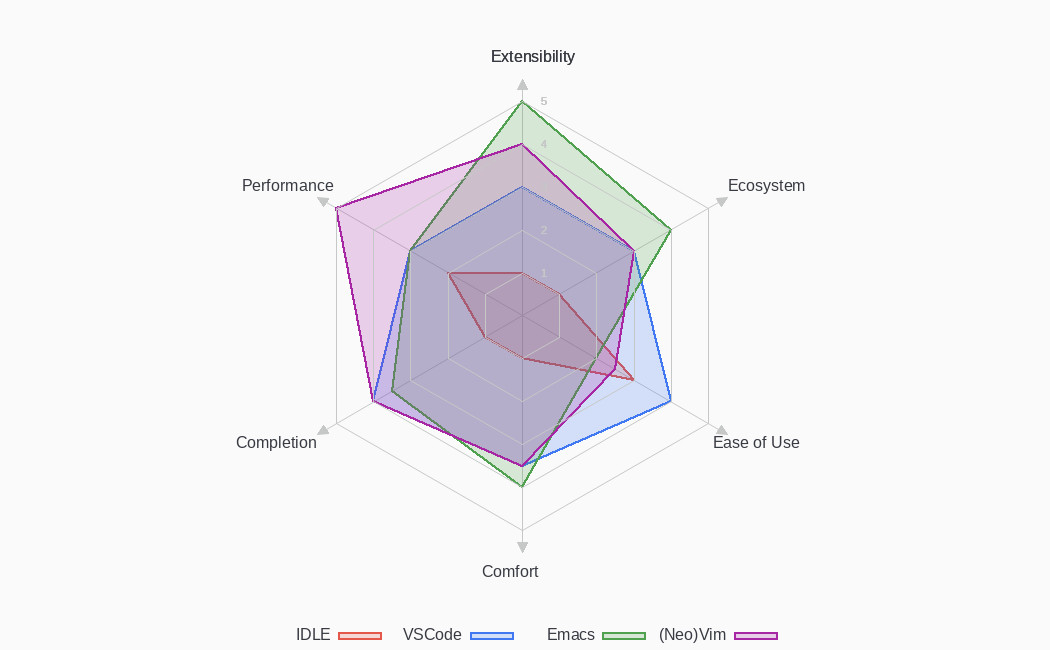
\includegraphics[width=.9\linewidth]{./misc/editor-comparison.jpeg}
\end{center}
\subsection{Why Emacs?}
\label{sec:org935a8ff}
Emacs is \href{https://www.eigenbahn.com/2020/01/12/emacs-is-no-editor}{not a text editor}, this is a common misnomer. It is far more apt to
describe Emacs as \emph{a Lisp machine providing a generic user-centric text
manipulation environment}. That's quite a mouthful.
In simpler terms one can think of Emacs as a platform for text-related
applications. It's a vague and generic definition because Emacs itself is
generic.

Good with text. How far does that go? A lot further than one initially thinks:
\begin{itemize}
\item \href{https://orgmode.org/}{Task planning}
\item \href{https://www.gnu.org/software/emacs/manual/html\_node/emacs/Dired.html}{File management}
\item \href{https://github.com/akermu/emacs-libvterm}{Terminal emulation}
\item \href{https://www.djcbsoftware.nl/code/mu/mu4e.html}{Email client}
\item \href{https://www.gnu.org/software/tramp/}{Remote server tool}
\item \href{https://magit.vc/}{Git frontend}
\item Web \href{https://github.com/pashky/restclient.el}{client}/\href{https://github.com/skeeto/emacs-web-server}{server}
\item and more\ldots{}
\end{itemize}

Ideally, one may use Emacs as \emph{the} interface to perform \texttt{input → transform →
output} cycles, i.e. form a bridge between the human mind and information
manipulation.

\subsubsection{The enveloping editor}
\label{sec:org5dbf8e9}
Emacs allows one to do more in one place than any other application. Why is this
good?
\begin{itemize}
\item Enables one to complete tasks with a consistent, standard set of keybindings,
GUI and editing methods --- learn once, use everywhere
\item Reduced context-switching
\item Compressing the stages of a project --- a more centralised workflow can progress
with greater ease
\item Integration between tasks previously relegated to different applications, but
with a common subject --- e.g. linking to an email in a to-do list
\end{itemize}

Emacs can be thought of as a platform within which various elements of your
workflow may settle, with the potential for rich integrations between them --- a
\emph{life} IDE if you will.

Today, many aspects of daily computer usage are split between different
applications which act like islands, but this often doesn't mirror how we
\emph{actually use} our computers. Emacs, if one goes down the rabbit hole, can give
users the power to bridge this gap.

\subsection{Notes for the unwary adventurer}
\label{sec:orga08e680}
If you like the look of this, that's marvellous, and I'm really happy that I've
made something which you may find interesting, however:
\begin{warning}
This config is \emph{insidious}. Copying the whole thing blindly can easily lead to
undesired effects. I recommend copying chunks instead.
\end{warning}

If you are so bold as to wish to steal bits of my config (or if I upgrade and
wonder why things aren't working), here's a list of sections which rely on
external setup (i.e. outside of this config).

Oh, did I mention that I started this config when I didn't know any \texttt{lisp}, and
this whole thing is a hack job? If you can suggest any improvements, please do
so, no matter how much criticism you include I'll appreciate it :)

\subsubsection{Extra Requirements}
\label{sec:org6cc7653}
The lovely \texttt{doom doctor} is good at diagnosing most missing things, but here are a
few extras.
\begin{itemize}
\item A \href{https://www.tug.org/texlive/}{\LaTeX{} Compiler} is required for the mathematics rendering performed in \href{https://orgmode.org/}{org},
and that wonderful pdf/html export we have going. I recommend \href{https://github.com/tectonic-typesetting/tectonic}{Tectonic}.
\item I use the \href{https://overpassfont.org/}{Overpass} font as a go-to sans serif.
It's used as my \texttt{doom-variable-pitch-font}
I have chosen it because it possesses a few characteristics I consider
desirable, namely:
\begin{itemize}
\item A clean, and legible style. Highway-style fonts tend to be designed to be
clear at a glance, and work well with a thicker weight, and this is inspired
by \emph{Highway Gothic}.
\item It's slightly quirky. Look at the diagonal cut on stems for example.
Helvetica is a masterful design, but I like a bit more pizzazz now and then.
\item \textbf{Note:} Alegreya is used for my latex export and writeroom mode configurations
\end{itemize}
\item I use my \href{https://github.com/shaunsingh/SFMono-Nerd-Font-Ligaturized}{patched SFMono} font as a go-to monospace.
I have chosen it because it possesses a few characteristics I consider
desirable, namely:
\begin{itemize}
\item Elegent characters, and good ligatures/unicode support
\item It fits will with the rest of my system
\end{itemize}
\item A few LSP servers. Take a look at \href{init.el}{init.el}' to see which modules have the \texttt{+lsp}
flag.
\item Gnuplot, used for \texttt{org-plot}.
\item A build of emacs with modules and xwidgets support. I also recommend the
native-comp flag with emacs28.
\end{itemize}

\section{Doom Configuration}
\label{sec:org57fbc0c}
\subsubsection{Modules}
\label{sec:orgc2ce7c6}
Doom has this lovely \emph{modular configuration base} that takes a lot of work out of
configuring Emacs. Each module (when enabled) can provide a list of packages to
install (on \texttt{doom sync}) and configuration to be applied. The modules can also
have flags applied to tweak their behaviour.

\begin{Code}
\begin{Verbatim}[]
\color{EFD}\EFcd{;;; }\EFct{init.el -*- lexical-binding: t; -*-}

\EFcd{;; }\EFct{This file controls what Doom modules are enabled and what order they load in.}
\EFcd{;; }\EFct{Press '}\textcolor[HTML]{b751b6}{K}\EFct{' on a module to view its documentation, and '}\textcolor[HTML]{b751b6}{gd}\EFct{' to browse its directory.}

\EFrdi{(}\EFk{doom!} \EFb{:completion}
       <<doom-completion>>

       \EFb{:ui}
       <<doom-ui>>

       \EFb{:editor}
       <<doom-editor>>

       \EFb{:emacs}
       <<doom-emacs>>

       \EFb{:term}
       <<doom-term>>

       \EFb{:checkers}
       <<doom-checkers>>

       \EFb{:tools}
       <<doom-tools>>

       \EFb{:os}
       <<doom-os>>

       \EFb{:lang}
       <<doom-lang>>

       \EFb{:email}
       <<doom-email>>

       \EFb{:app}
       <<doom-app>>

       \EFb{:config}
       <<doom-config>>
       \EFrdi{)}
\end{Verbatim}
\end{Code}

\begin{enumerate}
\item Structure
\label{sec:orgf6d3a56}
As you may have noticed by this point, this is a \href{https://en.wikipedia.org/wiki/Literate\_programming}{literate} configuration. Doom
has good support for this which we access though the \texttt{literate} module.

While we're in the \Verb{\color{EFD}\EFb{:config}} section, we'll use Dooms nicer defaults,
along with the bindings and smartparens behaviour (the flags aren't documented,
but they exist).
\begin{Code}
\begin{Verbatim}[]
\color{EFD}literate
\EFrdi{(}default +bindings +smartparens\EFrdi{)}
\end{Verbatim}
\end{Code}

\item Interface
\label{sec:org78d7407}
There's a lot that can be done to enhance Emacs' capabilities.
I reckon enabling half the modules Doom provides should do it.

\begin{Code}
\begin{Verbatim}[]
\color{EFD}\EFrdi{(}company                     \EFcd{; }\EFct{the ultimate code completion backend}
 +childframe\EFrdi{)}                \EFcd{; }\EFct{... when your children are better than you}
\EFcd{;;}\EFct{helm                       ; the *other* search engine for love and life}
\EFcd{;;}\EFct{ido                        ; the other *other* search engine...}
\EFcd{;;}\EFct{(ivy                       ; a search engine for love and life}
\EFcd{;; }\EFct{+icons                    ; ... icons are nice}
\EFcd{;; }\EFct{+prescient)               ; ... I know what I want(ed)}
\EFrdi{(}vertico +icons\EFrdi{)}             \EFcd{; }\EFct{the search engine of the future}
\end{Verbatim}
\end{Code}

\begin{Code}
\begin{Verbatim}[]
\color{EFD}\EFcd{;;}\EFct{deft                       ; notational velocity for Emacs}
doom                         \EFcd{; }\EFct{what makes DOOM look the way it does}
doom-dashboard               \EFcd{; }\EFct{a nifty splash screen for Emacs}
doom-quit                    \EFcd{; }\EFct{DOOM quit-message prompts when you quit Emacs}
\EFrdi{(}emoji +unicode\EFrdi{)}             \EFcd{; }\EFct{🙂}
\EFcd{;;}\EFct{fill-column                ; a `}\textcolor[HTML]{b751b6}{fill-column}\EFct{' indicator}
hl-todo                      \EFcd{; }\EFct{highlight }\textcolor[HTML]{986801}{\textbf{TODO}}\EFct{/}\textcolor[HTML]{e45649}{\textbf{FIXME}}\EFct{/}\textcolor[HTML]{50a14f}{\textbf{NOTE}}\EFct{/}\textcolor[HTML]{84888b}{\textbf{\textit{DEPRECATED}}}\EFct{/}\textcolor[HTML]{b751b6}{\textbf{HACK}}\EFct{/}\textcolor[HTML]{e45649}{\textbf{REVIEW}}
\EFcd{;;}\EFct{hydra                      ; quick documentation for related commands}
\EFcd{;;}\EFct{indent-guides              ; highlighted indent columns, notoriously slow}
\EFrdi{(}ligatures +extra\EFrdi{)}           \EFcd{; }\EFct{ligatures and symbols to make your code pretty again}
\EFcd{;;}\EFct{minimap                    ; show a map of the code on the side}
modeline                     \EFcd{; }\EFct{snazzy, Atom-inspired modeline, plus API}
 \EFcd{;;}\EFct{+light)                   ; the doom modeline is a bit much, the default is a bit little}
\EFcd{;;}\EFct{nav-flash                  ; blink the current line after jumping}
\EFcd{;;}\EFct{neotree                    ; a project drawer, like NERDTree for vim}
ophints                      \EFcd{; }\EFct{highlight the region an operation acts on}
\EFrdi{(}popup                       \EFcd{; }\EFct{tame sudden yet inevitable temporary windows}
 +all                        \EFcd{; }\EFct{catch all popups that start with an asterix}
 +defaults\EFrdi{)}                  \EFcd{; }\EFct{default popup rules}
\EFcd{;;}\EFct{(tabs                      ; an tab bar for Emacs}
\EFcd{;;  }\EFct{+centaur-tabs)           ; ... with prettier tabs}
treemacs                     \EFcd{; }\EFct{a project drawer, like neotree but cooler}
\EFcd{;;}\EFct{tree-sitter                ; ... sitting in a tree}
\EFcd{;;}\EFct{unicode                    ; extended unicode support for various languages}
vc-gutter                    \EFcd{; }\EFct{vcs diff in the fringe}
\EFcd{;;}\EFct{vi-tilde-fringe            ; fringe tildes to mark beyond EOB}
\EFcd{;;}\EFct{(window-select +numbers)   ; visually switch windows}
workspaces                   \EFcd{; }\EFct{tab emulation, persistence \& separate workspaces}
zen                          \EFcd{; }\EFct{distraction-free coding or writing}
\end{Verbatim}
\end{Code}

\begin{Code}
\begin{Verbatim}[]
\color{EFD}\EFrdi{(}evil +everywhere\EFrdi{)}           \EFcd{; }\EFct{come to the dark side, we have cookies}
file-templates               \EFcd{; }\EFct{auto-snippets for empty files}
fold                         \EFcd{; }\EFct{(nigh) universal code folding}
format                       \EFcd{; }\EFct{automated prettiness}
\EFcd{;;}\EFct{god                        ; run Emacs commands without modifier keys}
\EFcd{;;}\EFct{lispy                      ; vim for lisp, for people who don't like vim}
\EFcd{;;}\EFct{multiple-cursors           ; editing in many places at once}
\EFcd{;;}\EFct{objed                      ; text object editing for the innocent}
\EFcd{;;}\EFct{parinfer                   ; turn lisp into python, sort of}
\EFcd{;;}\EFct{rotate-text                ; cycle region at point between text candidates}
snippets                     \EFcd{; }\EFct{my elves. They type so I don't have to}
\EFcd{;;}\EFct{word-wrap                  ; soft wrapping with language-aware indent}
\end{Verbatim}
\end{Code}

\begin{Code}
\begin{Verbatim}[]
\color{EFD}\EFrdi{(}\EFc{dired} +icons\EFrdi{)}               \EFcd{; }\EFct{making dired pretty [functional]}
electric                     \EFcd{; }\EFct{smarter, keyword-based electric-indent}
\EFrdi{(}\EFc{ibuffer} +icons\EFrdi{)}             \EFcd{; }\EFct{interactive buffer management}
undo                         \EFcd{; }\EFct{persistent, smarter undo for your inevitable mistakes}
vc                           \EFcd{; }\EFct{version-control and Emacs, sitting in a tree}
\end{Verbatim}
\end{Code}

\begin{Code}
\begin{Verbatim}[]
\color{EFD}\EFcd{;;}\EFct{eshell                     ; the elisp shell that works everywhere}
\EFcd{;;}\EFct{shell                      ; simple shell REPL for Emacs}
\EFcd{;;}\EFct{term                       ; basic terminal emulator for Emacs}
vterm                        \EFcd{; }\EFct{the best terminal emulation in Emacs}
\end{Verbatim}
\end{Code}

\begin{Code}
\begin{Verbatim}[]
\color{EFD}syntax                       \EFcd{; }\EFct{tasing you for every semicolon you forget}
\EFrdi{(}\EFb{:if} \EFrdii{(}\EFc{executable-find} \EFs{"aspell"}\EFrdii{)} spell\EFrdi{)} \EFcd{; }\EFct{tasing you for misspelling mispelling}
\EFcd{;;}\EFct{grammar                    ; tasing grammar mistake every you make}
\end{Verbatim}
\end{Code}

\begin{Code}
\begin{Verbatim}[]
\color{EFD}\EFcd{;;}\EFct{ansible                    ; a crucible for infrastructure as code}
\EFcd{;;}\EFct{debugger                   ; }\textcolor[HTML]{e45649}{\textbf{FIXME}}\EFct{ stepping through code, to help you add bugs}
\EFcd{;;}\EFct{direnv                     ; be direct about your environment}
\EFcd{;;}\EFct{docker                     ; port everything to containers}
\EFcd{;;}\EFct{editorconfig               ; let someone else argue about tabs vs spaces}
\EFcd{;;}\EFct{ein                        ; tame Jupyter notebooks with emacs}
\EFcd{;;}\EFct{(eval +overlay)            ; run code, run (also, repls)}
\EFcd{;;}\EFct{gist                       ; interacting with github gists}
\EFrdi{(}lookup                      \EFcd{; }\EFct{helps you navigate your code and documentation}
 +dictionary                 \EFcd{; }\EFct{dictionary/thesaurus is nice}
 +docsets\EFrdi{)}                   \EFcd{; }\EFct{...or in Dash docsets locally}
lsp                          \EFcd{; }\EFct{Language Server Protocol}
\EFcd{;;}\EFct{macos                      ; MacOS-specific commands}
\EFrdi{(}\EFc{magit}                       \EFcd{; }\EFct{a git porcelain for Emacs}
 +forge\EFrdi{)}                     \EFcd{; }\EFct{interface with git forges}
\EFcd{;;}\EFct{make                       ; run make tasks from Emacs}
\EFcd{;;}\EFct{pass                       ; password manager for nerds}
pdf                          \EFcd{; }\EFct{pdf enhancements}
\EFcd{;;}\EFct{prodigy                    ; }\textcolor[HTML]{e45649}{\textbf{FIXME}}\EFct{ managing external services \& code builders}
\EFcd{;;}\EFct{rgb                        ; creating color strings}
\EFcd{;;}\EFct{taskrunner                 ; taskrunner for all your projects}
\EFcd{;;}\EFct{terraform                  ; infrastructure as code}
\EFcd{;;}\EFct{tmux                       ; an API for interacting with tmux}
\EFcd{;;}\EFct{upload                     ; map local to remote projects via ssh/ftp}
\end{Verbatim}
\end{Code}

\begin{Code}
\begin{Verbatim}[]
\color{EFD}\EFrdi{(}\EFb{:if} \EFv{IS-MAC} macos\EFrdi{)}           \EFcd{; }\EFct{improve compatibility with macOS}
\EFcd{;;}\EFct{tty                        ; improve the terminal Emacs experience}
\end{Verbatim}
\end{Code}

\item Language support
\label{sec:org5f0033f}
We can be rather liberal with enabling support for languages as the associated
packages/configuration are (usually) only loaded when first opening an
associated file.

\begin{Code}
\begin{Verbatim}[]
\color{EFD}\EFcd{;;}\EFct{agda                       ; types of types of types of types...}
\EFcd{;;}\EFct{beancount                  ; mind the GAAP}
\EFcd{;;}\EFct{cc                         ; C/C++/Obj-C madness}
\EFcd{;;}\EFct{clojure                    ; java with a lisp}
\EFcd{;;}\EFct{common-lisp                ; if you've seen one lisp, you've seen them all}
\EFcd{;;}\EFct{coq                        ; proofs-as-programs}
\EFcd{;;}\EFct{crystal                    ; ruby at the speed of c}
\EFcd{;;}\EFct{csharp                     ; unity, .NET, and mono shenanigans}
\EFcd{;;}\EFct{data                       ; config/data formats}
\EFcd{;;}\EFct{(dart +flutter)            ; paint ui and not much else}
\EFcd{;;}\EFct{dhall                      ; JSON with FP sprinkles}
\EFcd{;;}\EFct{elixir                     ; erlang done right}
\EFcd{;;}\EFct{elm                        ; care for a cup of TEA?}
emacs-lisp                   \EFcd{; }\EFct{drown in parentheses}
\EFcd{;;}\EFct{erlang                     ; an elegant language for a more civilized age}
\EFcd{;;}\EFct{ess                        ; emacs speaks statistics}
\EFcd{;;}\EFct{faust                      ; dsp, but you get to keep your soul}
\EFcd{;;}\EFct{fsharp                     ; ML stands for Microsoft's Language}
\EFcd{;;}\EFct{fstar                      ; (dependent) types and (monadic) effects and Z3}
\EFcd{;;}\EFct{gdscript                   ; the language you waited for}
\EFcd{;;}\EFct{(go +lsp)                  ; the hipster dialect}
\EFcd{;;}\EFct{(haskell +lsp)             ; a language that's lazier than I am}
\EFcd{;;}\EFct{hy                         ; readability of scheme w/ speed of python}
\EFcd{;;}\EFct{idris                      ;}
\EFcd{;;}\EFct{json                       ; At least it ain't XML}
\EFrdi{(}java +lsp\EFrdi{)}                  \EFcd{; }\EFct{the poster child for carpal tunnel syndrome}
\EFcd{;;}\EFct{(javascript +lsp)          ; all(hope(abandon(ye(who(enter(here))))))}
\EFcd{;;}\EFct{(julia +lsp)               ; Python, R, and MATLAB in a blender}
\EFcd{;;}\EFct{(kotlin +lsp)              ; a better, slicker Java(Script)}
\EFrdi{(}latex                       \EFcd{; }\EFct{writing papers in Emacs has never been so fun}
\EFcd{;; }\EFct{+fold                     ; fold the clutter away nicities}
 +cdlatex                    \EFcd{; }\EFct{quick maths symbols}
 +lsp\EFrdi{)}
\EFcd{;;}\EFct{lean                       ; proof that mathematicians need help}
\EFcd{;;}\EFct{factor                     ; for when scripts are stacked against you}
\EFcd{;;}\EFct{ledger                     ; an accounting system in Emacs}
\EFcd{;;}\EFct{(lua +lsp)                 ; one-based indices? one-based indices}
\EFcd{;;}\EFct{markdown                   ; writing docs for people to ignore}
\EFcd{;;}\EFct{nim                        ; python + lisp at the speed of c}
\EFcd{;;}\EFct{nix                        ; I hereby declare "nix geht mehr!"}
\EFcd{;;}\EFct{ocaml                      ; an objective camel}
\EFrdi{(}org                         \EFcd{; }\EFct{organize your plain life in plain text}
 +pretty                     \EFcd{; }\EFct{yessss my pretties! (nice unicode symbols)}
 +dragndrop                  \EFcd{; }\EFct{drag \& drop files/images into org buffers}
 \EFcd{;;}\EFct{+hugo                     ; use Emacs for hugo blogging}
 \EFcd{;;}\EFct{+noter                    ; enhanced PDF notetaking}
 +jupyter                    \EFcd{; }\EFct{ipython/jupyter support for babel}
 +pandoc                     \EFcd{; }\EFct{export-with-pandoc support}
 +gnuplot                    \EFcd{; }\EFct{who doesn't like pretty pictures}
 +pomodoro                   \EFcd{; }\EFct{be fruitful with the tomato technique}
 +present                    \EFcd{; }\EFct{using org-mode for presentations}
 +roam2\EFrdi{)}                     \EFcd{; }\EFct{wander around notes}
\EFcd{;;}\EFct{php                        ; perl's insecure younger brother}
\EFcd{;;}\EFct{plantuml                   ; diagrams for confusing people more}
\EFcd{;;}\EFct{purescript                 ; javascript, but functional}
\EFrdi{(}python +lsp +pyright\EFrdi{)}       \EFcd{; }\EFct{beautiful is better than ugly}
\EFcd{;;}\EFct{qt                         ; the '}\textcolor[HTML]{b751b6}{cutest}\EFct{' gui framework ever}
\EFcd{;;}\EFct{racket                     ; a DSL for DSLs}
\EFcd{;;}\EFct{raku                       ; the artist formerly known as perl6}
\EFcd{;;}\EFct{rest                       ; Emacs as a REST client}
\EFcd{;;}\EFct{rst                        ; ReST in peace}
\EFcd{;;}\EFct{(ruby +rails)              ; 1.step \{|i| p "Ruby is \#\{i.even? ? '}\textcolor[HTML]{b751b6}{love}\EFct{' : '}\textcolor[HTML]{b751b6}{life}\EFct{'\}"\}}
\EFcd{;;}\EFct{(rust +lsp)                ; Fe2O3.unwrap().unwrap().unwrap().unwrap()}
\EFcd{;;}\EFct{scala                      ; java, but good}
\EFcd{;;}\EFct{scheme                     ; a fully conniving family of lisps}
\EFcd{;;}\EFct{sh                         ; she sells \{ba,z,fi\}sh shells on the C xor}
\EFcd{;;}\EFct{sml                        ; no, the /other/ ML}
\EFcd{;;}\EFct{solidity                   ; do you need a blockchain? No.}
\EFcd{;;}\EFct{swift                      ; who asked for emoji variables?}
\EFcd{;;}\EFct{terra                      ; Earth and Moon in alignment for performance.}
\EFcd{;;}\EFct{web                        ; the tubes}
\EFcd{;;}\EFct{yaml                       ; JSON, but readable}
\EFcd{;;}\EFct{zig                        ; C, but simpler}
\end{Verbatim}
\end{Code}

\item Everything in Emacs
\label{sec:org397da39}
It's just too convenient being able to have everything in Emacs.
I couldn't resist the Email and Feed modules.
\begin{Code}
\begin{Verbatim}[]
\color{EFD}\EFrdi{(}\EFb{:if} \EFrdii{(}\EFc{executable-find} \EFs{"mu"}\EFrdii{)} \EFrdii{(}\EFf{mu4e} +org +gmail\EFrdii{)}\EFrdi{)}
\EFcd{;;}\EFct{notmuch}
\EFcd{;;}\EFct{(wanderlust +gmail)}
\end{Verbatim}
\end{Code}

\begin{Code}
\begin{Verbatim}[]
\color{EFD}\EFcd{;;}\EFct{calendar                   ; A dated approach to timetabling}
\EFcd{;;}\EFct{emms                       ; Multimedia in Emacs is music to my ears}
\EFcd{;;}\EFct{everywhere                 ; *leave* Emacs!? You must be joking.}
\EFcd{;;}\EFct{irc                          ; how neckbeards socialize}
\EFcd{;;}\EFct{(rss +org)                   ; emacs as an RSS reader}
\EFcd{;;}\EFct{twitter                    ; twitter client https://twitter.com/vnought}
\end{Verbatim}
\end{Code}
\end{enumerate}

\subsubsection{Packages}
\label{sec:org894afd0}
Unlike most literate configurations I \sout{am lazy} like to keep all my packages in
one place
\begin{Code}
\begin{Verbatim}[]
\color{EFD}\EFcd{;; }\EFct{-*- no-byte-compile: t; -*-}
\EFcd{;;; }\EFct{\$DOOMDIR/packages.el}

\EFcd{;;}\EFct{org}
<<org>>

\EFcd{;;}\EFct{latex}
<<latex>>

\EFcd{;;}\EFct{markdown and html}
<<web>>

\EFcd{;;}\EFct{looks}
<<looks>>

\EFcd{;;}\EFct{emacs additions}
<<emacs>>

\EFcd{;;}\EFct{lsp}
<<lsp>>

\EFcd{;;}\EFct{fun}
<<fun>>
\end{Verbatim}
\end{Code}

\begin{enumerate}
\item Org:
\label{sec:org450bd80}
The majority of my work in emacs is done in org mode, even this configuration
was written in org! It makes sense that the majority of my packages are for
tweaking org then
\begin{Code}
\begin{Verbatim}[]
\color{EFD}\EFrdi{(}\EFk{package!} org-appear\EFrdi{)}
\EFrdi{(}\EFk{package!} doct \EFb{:recipe} \EFrdii{(}\EFb{:host} github \EFb{:repo} \EFs{"progfolio/doct"}\EFrdii{)}\EFrdi{)}
\EFrdi{(}\EFk{package!} org-padding \EFb{:recipe} \EFrdii{(}\EFb{:host} github \EFb{:repo} \EFs{"TonCherAmi/org-padding"}\EFrdii{)}\EFrdi{)}
\EFrdi{(}\EFk{package!} org-ol-tree \EFb{:recipe} \EFrdii{(}\EFb{:host} github \EFb{:repo} \EFs{"Townk/org-ol-tree"}\EFrdii{)}\EFrdi{)}
\EFrdi{(}\EFk{package!} org-pretty-table \EFb{:recipe} \EFrdii{(}\EFb{:host} github \EFb{:repo} \EFs{"Fuco1/org-pretty-table"}\EFrdii{)}\EFrdi{)}
\EFrdi{(}\EFk{package!} org-roam-ui \EFb{:recipe} \EFrdii{(}\EFb{:host} github \EFb{:repo} \EFs{"org-roam/org-roam-ui"} \EFb{:files} \EFrdiii{(}\EFs{"*.el"} \EFs{"out"}\EFrdiii{)}\EFrdii{)}\EFrdi{)}
\EFrdi{(}\EFk{package!} org-pandoc-import
  \EFb{:recipe} \EFrdii{(}\EFb{:host} github
           \EFb{:repo} \EFs{"tecosaur/org-pandoc-import"}
           \EFb{:files} \EFrdiii{(}\EFs{"*.el"} \EFs{"filters"} \EFs{"preprocessors"}\EFrdiii{)}\EFrdii{)}\EFrdi{)}
\end{Verbatim}
\end{Code}

\item \LaTeX:
\label{sec:org308a909}
When I'm not working in org, I'm probably exporting it to latex. Lets adjust
that a bit too
\begin{Code}
\begin{Verbatim}[]
\color{EFD}\EFcd{;;}\EFct{(package! org-fragtog)}
\EFrdi{(}\EFk{package!} aas \EFb{:recipe} \EFrdii{(}\EFb{:host} github \EFb{:repo} \EFs{"ymarco/auto-activating-snippets"}\EFrdii{)}\EFrdi{)}
\EFrdi{(}\EFk{package!} laas \EFb{:recipe} \EFrdii{(}\EFb{:host} github \EFb{:repo} \EFs{"tecosaur/LaTeX-auto-activating-snippets"}\EFrdii{)}\EFrdi{)}
\EFrdi{(}\EFk{package!} engrave-faces \EFb{:recipe} \EFrdii{(}\EFb{:host} github \EFb{:repo} \EFs{"tecosaur/engrave-faces"}\EFrdii{)}\EFrdi{)}
\EFrdi{(}\EFk{package!} math-preview\EFrdi{)}
\end{Verbatim}
\end{Code}

\item Web:
\label{sec:org88a5c70}
Sometimes I need to use markdown too. \textbf{Note:} emacs-webkit is temporarily disabled
because of its refusal to work without requiring org
\begin{Code}
\begin{Verbatim}[]
\color{EFD}\EFrdi{(}\EFk{package!} ox-gfm\EFrdi{)}
\EFrdi{(}\EFk{package!} websocket\EFrdi{)}
\EFcd{;;}\EFct{(package! webkit}
\EFcd{;;          }\EFct{:recipe (:host github}
\EFcd{;;                   }\EFct{:repo "akirakyle/emacs-webkit"}
\EFcd{;;                   }\EFct{:branch "main"}
\EFcd{;;                   }\EFct{:files (:defaults "*.js" "*.css" "*.so" "*.nix")}
\EFcd{;;                   }\EFct{:pre-build (("nix-shell" "shell.nix" "--command make"))))}
\end{Verbatim}
\end{Code}

\item Looks:
\label{sec:org411cec4}
Making emacs look good is first priority, actually working in it is second
\begin{Code}
\begin{Verbatim}[]
\color{EFD}\EFrdi{(}\EFk{unpin!} doom-themes\EFrdi{)}
\EFrdi{(}\EFk{unpin!} doom-modeline\EFrdi{)}
\EFrdi{(}\EFk{package!} solaire-mode \EFb{:disable} t\EFrdi{)}
\EFrdi{(}\EFk{package!} ox-chameleon \EFb{:recipe} \EFrdii{(}\EFb{:host} github \EFb{:repo} \EFs{"tecosaur/ox-chameleon"}\EFrdii{)}\EFrdi{)}
\end{Verbatim}
\end{Code}

\item Emacs Tweaks:
\label{sec:orgdd5b2fc}
Emacs is missing just a few packages that I need to make it my OS. Specifically,
screenshot capabilities are nice, and using the same dictionaries accross
\sout{operating systems} bootloaders would be nice too!
\begin{Code}
\begin{Verbatim}[]
\color{EFD}\EFcd{;;}\EFct{(package! vlf :recipe (:host github :repo "m00natic/vlfi" :files ("*.el")))}
\EFrdi{(}\EFk{package!} screenshot \EFb{:recipe} \EFrdii{(}\EFb{:host} github \EFb{:repo} \EFs{"tecosaur/screenshot"}\EFrdii{)}\EFrdi{)}
\EFrdi{(}\EFk{package!} lexic \EFb{:recipe} \EFrdii{(}\EFb{:host} github \EFb{:repo} \EFs{"tecosaur/lexic"}\EFrdii{)}\EFrdi{)}
\end{Verbatim}
\end{Code}

\item LSP:
\label{sec:org862d50b}
I like to live life on the edge
\begin{Code}
\begin{Verbatim}[]
\color{EFD}\EFrdi{(}\EFk{unpin!} lsp-ui\EFrdi{)}
\EFrdi{(}\EFk{unpin!} lsp-mode\EFrdi{)}
\end{Verbatim}
\end{Code}

\item Fun:
\label{sec:org714da53}
We do a little trolling
\begin{Code}
\begin{Verbatim}[]
\color{EFD}\EFrdi{(}\EFk{package!} xkcd\EFrdi{)}
\EFrdi{(}\EFk{package!} keycast\EFrdi{)}
\EFrdi{(}\EFk{package!} \EFv{selectric-mode}\EFrdi{)}
\end{Verbatim}
\end{Code}
\end{enumerate}

\section{Basic Configuration}
\label{sec:org55df5aa}
Make this file run (slightly) faster with lexical binding
\begin{Code}
\begin{Verbatim}[]
\color{EFD}\EFcd{;;; }\EFct{config.el -*- lexical-binding: t; -*-}
\end{Verbatim}
\end{Code}

I want to run emacs28's new native-compiler with -O3, if available
\begin{Code}
\begin{Verbatim}[]
\color{EFD}\EFrdi{(}\EFk{when} \EFhq{'}\EFv{native-comp-compiler-options}
                 \EFrdii{(}\EFk{setq} \EFv{native-comp-compiler-options} \EFhq{'}\EFrdiii{(}\EFs{"-O3"}\EFrdiii{)}\EFrdii{)}\EFrdi{)}
\end{Verbatim}
\end{Code}

\subsection{Personal information}
\label{sec:org2378ac1}
Of course we need to tell emacs who I am
\begin{Code}
\begin{Verbatim}[]
\color{EFD}\EFrdi{(}\EFk{setq} \EFv{user-full-name} \EFs{"Shaurya Singh"}
      \EFv{user-mail-address} \EFs{"shaunsingh0207@gmail.com"}\EFrdi{)}
\end{Verbatim}
\end{Code}

\subsection{Authinfo}
\label{sec:org7f1ce9a}
I frequently delete my \texttt{\textasciitilde{}/.emacs.d} for fun, so having authinfo in a seperate file
sounds like a good idea
\begin{Code}
\begin{Verbatim}[]
\color{EFD}\EFrdi{(}\EFk{setq} \EFv{auth-sources} \EFhq{'}\EFrdii{(}\EFs{"\char126{}/.authinfo.gpg"}\EFrdii{)}
      \EFv{auth-source-cache-expiry} nil\EFrdi{)} \EFcd{; }\EFct{default is 7200 (2h)}
\end{Verbatim}
\end{Code}

\subsection{Emacsclient}
\label{sec:org0019e99}
mu4e is a bit finicky with emacsclient, and org takes forever to load. The
solution? Use tecosaurs greedy daemon startup
\begin{Code}
\begin{Verbatim}[]
\color{EFD}\EFrdi{(}\EFk{defun} \EFf{greedily-do-daemon-setup} \EFrdii{(}\EFrdii{)}
  \EFrdii{(}\EFc{require} \EFhq{'}\EFc{org}\EFrdii{)}
  \EFrdii{(}\EFc{require} \EFhq{'}\EFc{vertico}\EFrdii{)}
  \EFrdii{(}\EFc{require} \EFhq{'}\EFc{consult}\EFrdii{)}
  \EFrdii{(}\EFc{require} \EFhq{'}\EFc{marginalia}\EFrdii{)}
  \EFrdii{(}\EFk{when} \EFrdiii{(}\EFc{require} \EFhq{'}\EFc{mu4e} nil t\EFrdiii{)}
    \EFrdiii{(}\EFk{setq} mu4e-confirm-quit t\EFrdiii{)}
    \EFrdiii{(}\EFk{setq} +mu4e-lock-greedy t\EFrdiii{)}
    \EFrdiii{(}\EFk{setq} +mu4e-lock-relaxed t\EFrdiii{)}
    \EFrdiii{(}+mu4e-lock-add-watcher\EFrdiii{)}
    \EFrdiii{(}\EFk{when} \EFrdiv{(}+mu4e-lock-available t\EFrdiv{)}
      \EFrdiv{(}mu4e\char126{}start\EFrdiv{)}\EFrdiii{)}\EFrdii{)}\EFrdi{)}

\EFrdi{(}\EFk{when} \EFrdii{(}\EFc{daemonp}\EFrdii{)}
  \EFrdii{(}\EFc{add-hook} \EFhq{'}\EFv{emacs-startup-hook} \EFhq{\#'}\EFhs{greedily-do-daemon-setup}\EFrdii{)}
  \EFrdii{(}\EFc{add-hook} \EFhq{'}\EFv{emacs-startup-hook} \EFhq{\#'}\EFhs{init-mixed-pitch-h}\EFrdii{)}\EFrdi{)}
\end{Verbatim}
\end{Code}

\subsection{Shell}
\label{sec:org619b7a0}
I use the fish shell. If you use zsh/bash, be sure to change this
\begin{Code}
\begin{Verbatim}[]
\color{EFD}\EFrdi{(}\EFk{setq} \EFv{explicit-shell-file-name} \EFrdii{(}\EFc{executable-find} \EFs{"fish"}\EFrdii{)}\EFrdi{)}
\end{Verbatim}
\end{Code}

\subsubsection{Vterm}
\label{sec:org30faf95}
Vterm is my terminal emulator of choice. We can tell it to use ligatures, and also tell it to compile automatically
Vterm clearly wins the terminal war. Also doesn't need much configuration out of
the box, although the shell integration does. You can find that in \texttt{\textasciitilde{}/.config/fish/config.fish}
\begin{enumerate}
\item Always compile
\label{sec:org3bebe54}
Fixes a weird bug with native-comp
\begin{Code}
\begin{Verbatim}[]
\color{EFD}\EFrdi{(}\EFk{setq} vterm-always-compile-module t\EFrdi{)}
\end{Verbatim}
\end{Code}

\item Kill buffer
\label{sec:orga4e7d0f}
If the process exits, kill the \texttt{vterm} buffer
\begin{Code}
\begin{Verbatim}[]
\color{EFD}\EFrdi{(}\EFk{setq} vterm-kill-buffer-on-exit t\EFrdi{)}
\end{Verbatim}
\end{Code}

\item Functions
\label{sec:org42c293e}
Useful functions for the shell-side integration provided by vterm.
\begin{Code}
\begin{Verbatim}[]
\color{EFD}\EFrdi{(}\EFk{after!} vterm
  \EFrdii{(}\EFk{setf} \EFrdiii{(}\EFc{alist-get} \EFs{"magit-status"} vterm-eval-cmds nil nil \EFhq{\#'}\EFhs{equal}\EFrdiii{)}
        \EFhq{'}\EFrdiii{(}\EFrdiv{(}\EFk{lambda} \EFrdi{(}path\EFrdi{)}
            \EFrdi{(}\EFc{magit-status} path\EFrdi{)}\EFrdiv{)}\EFrdiii{)}\EFrdii{)}\EFrdi{)}
\end{Verbatim}
\end{Code}

\item Ligatures
\label{sec:orgf1f281b}
Use ligatures from within vterm (and eshell), we do this by redefining the variable where \emph{not} to show ligatures
\begin{Code}
\begin{Verbatim}[]
\color{EFD}\EFrdi{(}\EFk{setq} \EFv{+ligatures-in-modes} t\EFrdi{)}
\end{Verbatim}
\end{Code}
\end{enumerate}

\subsection{Fonts}
\label{sec:org4a92ea3}
\begin{figure}[!htb]
	  \centering
	  \includegraphics[scale=0.4]{/Users/shauryasingh/.emacs.d/.local/cache/xkcd/590.png}
  \caption*{\label{xkcd:590} \textbf{Papyrus} I secretly, deep in my guilty heart, like Papyrus and don't care if it's overused. [Cue hate mail in beautifully-kerned Helvetica.]}
	\end{figure}

I like the apple fonts for programming, so I'll go with Liga SFMono Nerd Font. I
prefer a rounder font for plain text, so I'll go with Overpass for that. I have a retina display as well, so lets keep the fonts light.
\begin{Code}
\begin{Verbatim}[]
\color{EFD}\EFcd{;;}\EFct{fonts}
\EFrdi{(}\EFk{setq} \EFv{doom-font} \EFrdii{(}\EFc{font-spec} \EFb{:family} \EFs{"Liga SFMono Nerd Font"} \EFb{:size} \EFhn{14}\EFrdii{)}
      \EFv{doom-big-font} \EFrdii{(}\EFc{font-spec} \EFb{:family} \EFs{"Liga SFMono Nerd Font"} \EFb{:size} \EFhn{20}\EFrdii{)}
      \EFv{doom-variable-pitch-font} \EFrdii{(}\EFc{font-spec} \EFb{:family} \EFs{"Overpass"} \EFb{:size} \EFhn{16}\EFrdii{)}
      \EFv{doom-unicode-font} \EFrdii{(}\EFc{font-spec} \EFb{:family} \EFs{"Liga SFMono Nerd Font"}\EFrdii{)}
      \EFv{doom-serif-font} \EFrdii{(}\EFc{font-spec} \EFb{:family} \EFs{"Liga SFMono Nerd Font"} \EFb{:weight} \EFhq{'}\EFhs{light}\EFrdii{)}\EFrdi{)}
\end{Verbatim}
\end{Code}

For mixed pitch, I would go with something comfier. I like Alegreya, so lets go with that
\begin{Code}
\begin{Verbatim}[]
\color{EFD}\EFcd{;;}\EFct{mixed pitch modes}
\EFrdi{(}\EFk{defvar} \EFv{mixed-pitch-modes} \EFhq{'}\EFrdii{(}org-mode LaTeX-mode markdown-mode gfm-mode Info-mode\EFrdii{)}
  \EFd{"Modes that `}\textcolor[HTML]{b751b6}{\textit{mixed-pitch-mode}}\EFd{' should be enabled in, but only after UI initialisation."}\EFrdi{)}
\EFrdi{(}\EFk{defun} \EFf{init-mixed-pitch-h} \EFrdii{(}\EFrdii{)}
  \EFd{"Hook `}\textcolor[HTML]{b751b6}{\textit{mixed-pitch-mode}}\EFd{' into each mode in `}\textcolor[HTML]{b751b6}{\textit{mixed-pitch-modes}}\EFd{'.
Also immediately enables `}\textcolor[HTML]{b751b6}{\textit{mixed-pitch-modes}}\EFd{' if currently in one of the modes."}
  \EFrdii{(}\EFk{when} \EFrdiii{(}\EFc{memq} \EFv{major-mode} \EFv{mixed-pitch-modes}\EFrdiii{)}
    \EFrdiii{(}\EFv{mixed-pitch-mode} \EFhn{1}\EFrdiii{)}\EFrdii{)}
  \EFrdii{(}\EFk{dolist} \EFrdiii{(}hook \EFv{mixed-pitch-modes}\EFrdiii{)}
    \EFrdiii{(}\EFc{add-hook} \EFrdiv{(}\EFc{intern} \EFrdi{(}\EFc{concat} \EFrdii{(}\EFc{symbol-name} hook\EFrdii{)} \EFs{"-hook"}\EFrdi{)}\EFrdiv{)} \EFhq{\#'}\EFv{mixed-pitch-mode}\EFrdiii{)}\EFrdii{)}\EFrdi{)}
\EFrdi{(}\EFc{add-hook} \EFhq{'}\EFv{doom-init-ui-hook} \EFhq{\#'}\EFhs{init-mixed-pitch-h}\EFrdi{)}
\EFrdi{(}\EFk{add-hook!} \EFhq{'}\EFv{org-mode-hook} \EFhq{\#'}\EFv{+org-pretty-mode}\EFrdi{)} \EFcd{;}\EFct{enter mixed pitch mode in org mode}

\EFcd{;;}\EFct{set mixed pitch font}
 \EFrdi{(}\EFk{after!} mixed-pitch
  \EFrdii{(}\EFk{defface} \EFv{variable-pitch-serif}
    \EFhq{'}\EFrdiii{(}\EFrdiv{(}t \EFrdi{(}\EFb{:family} \EFs{"serif"}\EFrdi{)}\EFrdiv{)}\EFrdiii{)}
    \EFd{"A variable-pitch face with serifs."}
    \EFb{:group} \EFhq{'}\EFhs{basic-faces}\EFrdii{)}
  \EFrdii{(}\EFk{setq} \EFv{mixed-pitch-set-height} t\EFrdii{)}
  \EFrdii{(}\EFk{setq} variable-pitch-serif-font \EFrdiii{(}\EFc{font-spec} \EFb{:family} \EFs{"Alegreya"} \EFb{:size} \EFhn{16}\EFrdiii{)}\EFrdii{)}
  \EFrdii{(}\EFc{set-face-attribute} \EFhq{'}\EFhs{variable-pitch-serif} nil \EFb{:font} variable-pitch-serif-font\EFrdii{)}
  \EFrdii{(}\EFk{defun} \EFf{mixed-pitch-serif-mode} \EFrdiii{(}\EFt{\&optional} arg\EFrdiii{)}
    \EFd{"Change the default face of the current buffer to a serifed variable pitch, while keeping some faces fixed pitch."}
    \EFrdiii{(}\EFk{interactive}\EFrdiii{)}
    \EFrdiii{(}\EFk{let} \EFrdiv{(}\EFrdi{(}\EFv{mixed-pitch-face} \EFhq{'}\EFhs{variable-pitch-serif}\EFrdi{)}\EFrdiv{)}
      \EFrdiv{(}\EFv{mixed-pitch-mode} \EFrdi{(}\EFk{or} arg \EFhq{'}\EFhs{toggle}\EFrdi{)}\EFrdiv{)}\EFrdiii{)}\EFrdii{)}\EFrdi{)}
\end{Verbatim}
\end{Code}

Harfbuzz is missing the beautiful ff ffi ffj ffl fft fi fj ft Th ligatures,
lets add those back in with the help of composition-function-table

\begin{Code}
\begin{Verbatim}[]
\color{EFD}\EFrdi{(}\EFc{set-char-table-range} \EFv{composition-function-table} ?f \EFhq{'}\EFrdii{(}\EFrdiii{[}\EFs{"}\textcolor[HTML]{4078f2}{\textbf{\char92{}\char92{}}}\textcolor[HTML]{4078f2}{\textbf{(?:}}\EFs{ff?[fijlt]}\textcolor[HTML]{4078f2}{\textbf{\char92{}\char92{}}}\textcolor[HTML]{4078f2}{\textbf{)}}\EFs{"} \EFhn{0} font-shape-gstring\EFrdiii{]}\EFrdii{)}\EFrdi{)}
\EFrdi{(}\EFc{set-char-table-range} \EFv{composition-function-table} ?T \EFhq{'}\EFrdii{(}\EFrdiii{[}\EFs{"}\textcolor[HTML]{4078f2}{\textbf{\char92{}\char92{}}}\textcolor[HTML]{4078f2}{\textbf{(?:}}\EFs{Th}\textcolor[HTML]{4078f2}{\textbf{\char92{}\char92{}}}\textcolor[HTML]{4078f2}{\textbf{)}}\EFs{"} \EFhn{0} font-shape-gstring\EFrdiii{]}\EFrdii{)}\EFrdi{)}
\end{Verbatim}
\end{Code}

Just in case the fonts aren't there, lets add check to notify the user of the
issue. Seems like I forget ot install fonts every time I switch between \sout{distros}
emacs bootloaders
\begin{Code}
\begin{Verbatim}[]
\color{EFD}\EFrdi{(}\EFk{defvar} \EFv{required-fonts} \EFhq{'}\EFrdii{(}\EFs{"Overpass"} \EFs{"Liga SFMono Nerd Font"} \EFs{"Alegreya"} \EFrdii{)}\EFrdi{)}
\EFrdi{(}\EFk{defvar} \EFv{available-fonts}
  \EFrdii{(}\EFc{delete-dups} \EFrdiii{(}\EFk{or} \EFrdiv{(}\EFc{font-family-list}\EFrdiv{)}
                   \EFrdiv{(}\EFc{split-string} \EFrdi{(}\EFc{shell-command-to-string} \EFs{"fc-list : family"}\EFrdi{)}
                                 \EFs{"[,\char92{}n]"}\EFrdiv{)}\EFrdiii{)}\EFrdii{)}\EFrdi{)}
\EFrdi{(}\EFk{defvar} \EFv{missing-fonts}
  \EFrdii{(}\EFc{delq} nil \EFrdiii{(}\EFc{mapcar}
             \EFrdiv{(}\EFk{lambda} \EFrdi{(}font\EFrdi{)}
               \EFrdi{(}\EFk{unless} \EFrdii{(}\EFc{delq} nil \EFrdiii{(}\EFc{mapcar} \EFrdiv{(}\EFk{lambda} \EFrdi{(}f\EFrdi{)}
                           \EFrdi{(}\EFf{string-match-p} \EFrdii{(}\EFc{format} \EFs{"\char94{}\%s\$"} font\EFrdii{)} f\EFrdi{)}\EFrdiv{)}
                                         \EFv{available-fonts}\EFrdiii{)}\EFrdii{)}
                                         font\EFrdi{)}\EFrdiv{)}
                                         \EFv{required-fonts}\EFrdiii{)}\EFrdii{)}\EFrdi{)}
\EFrdi{(}\EFk{if} \EFv{missing-fonts}
    \EFrdii{(}\EFc{pp-to-string}
     \EFhq{`}\EFrdiii{(}\EFk{unless} \EFv{noninteractive}
        \EFrdiv{(}\EFk{add-hook!} \EFhq{'}\EFv{doom-init-ui-hook}
          \EFrdi{(}\EFc{run-at-time} nil nil
                       \EFrdii{(}\EFk{lambda} \EFrdiii{(}\EFrdiii{)}
                         \EFrdiii{(}\EFc{message} \EFs{"\%s missing the following fonts: \%s"}
                                  \EFrdiv{(}\EFc{propertize} \EFs{"Warning!"} \EFhq{'}\EFhs{face} \EFhq{'}\EFrdi{(}bold warning\EFrdi{)}\EFrdiv{)}
                                  \EFrdiv{(}\EFc{mapconcat} \EFrdi{(}\EFk{lambda} \EFrdii{(}font\EFrdii{)}
                                               \EFrdii{(}\EFc{propertize} font \EFhq{'}\EFhs{face} \EFhq{'}\EFv{font-lock-variable-name-face}\EFrdii{)}\EFrdi{)}
                                             \EFhq{'},\EFv{missing-fonts}
                                             \EFs{", "}\EFrdiv{)}\EFrdiii{)}
                         \EFrdiii{(}\EFc{sleep-for} \EFhn{0.5}\EFrdiii{)}\EFrdii{)}\EFrdi{)}\EFrdiv{)}\EFrdiii{)}\EFrdii{)}
  \EFs{";; No missing fonts detected"}\EFrdi{)}
\end{Verbatim}
\end{Code}

\begin{Code}
\begin{Verbatim}[]
\color{EFD}<<detect-missing-fonts\EFrdi{(}\EFrdi{)}>>
\end{Verbatim}
\end{Code}

\subsection{Themes}
\label{sec:orge1bb457}
Right now I'm using nord, but I use doom-one-light sometimes
\begin{Code}
\begin{Verbatim}[]
\color{EFD}\EFrdi{(}\EFk{setq} \EFv{doom-theme} \EFhq{'}\EFhs{doom-one-light}\EFrdi{)}
\EFrdi{(}\EFk{setq} \EFv{doom-one-light-padded-modeline} t\EFrdi{)}
\EFcd{;;}\EFct{(setq doom-theme 'doom-nord)}
\EFcd{;;}\EFct{(setq doom-nord-padded-modeline t)}
\end{Verbatim}
\end{Code}

\subsection{Very large files}
\label{sec:orgc148442}
Emacs gets super slow with large files, this helps with that
\begin{Code}
\begin{Verbatim}[]
\color{EFD}\EFcd{;;}\EFct{(use-package! vlf-setup}
  \EFcd{;;}\EFct{:defer-incrementally vlf-tune vlf-base vlf-write vlf-search vlf-occur vlf-follow vlf-ediff vlf)}
\end{Verbatim}
\end{Code}

\subsection{Company}
\label{sec:org5b6b040}
I think company is a bit too quick to recommend some stuff
\begin{Code}
\begin{Verbatim}[]
\color{EFD}\EFrdi{(}\EFk{after!} company
   \EFrdii{(}\EFk{setq} \EFv{company-idle-delay} \EFhn{0.1}
      \EFv{company-minimum-prefix-length} \EFhn{1}
      \EFv{company-selection-wrap-around} t
      \EFv{company-require-match} \EFhq{'}\EFhs{never}
      company-dabbrev-downcase nil
      company-dabbrev-ignore-case t
      company-dabbrev-other-buffers nil
      \EFv{company-tooltip-limit} \EFhn{5}
      \EFv{company-tooltip-minimum-width} \EFhn{50}\EFrdii{)}\EFrdi{)}
\EFrdi{(}\EFf{set-company-backend!}
  \EFhq{'}\EFrdii{(}text-mode
    markdown-mode
    gfm-mode\EFrdii{)}
  \EFhq{'}\EFrdii{(}\EFb{:seperate}
    company-yasnippet
    company-ispell
    company-files\EFrdii{)}\EFrdi{)}

\EFcd{;;}\EFct{nested snippets}
\EFrdi{(}\EFk{setq} \EFv{yas-triggers-in-field} t\EFrdi{)}
\end{Verbatim}
\end{Code}

Lets add some snippets for latex
\begin{Code}
\begin{Verbatim}[]
\color{EFD}\EFrdi{(}\EFk{use-package!} aas
  \EFb{:commands} \EFv{aas-mode}\EFrdi{)}

\EFrdi{(}\EFk{use-package!} laas
  \EFb{:hook} \EFrdii{(}\EFc{LaTeX-mode} . \EFv{laas-mode}\EFrdii{)}
  \EFb{:config}
  \EFrdii{(}\EFk{defun} \EFf{laas-tex-fold-maybe} \EFrdiii{(}\EFrdiii{)}
    \EFrdiii{(}\EFk{unless} \EFrdiv{(}\EFc{equal} \EFs{"/"} \EFv{aas-transient-snippet-key}\EFrdiv{)}
      \EFrdiv{(}\EFf{+latex-fold-last-macro-a}\EFrdiv{)}\EFrdiii{)}\EFrdii{)}
  \EFrdii{(}\EFc{add-hook} \EFhq{'}\EFhs{org-mode} \EFhq{\#'}\EFv{laas-mode}\EFrdii{)}
  \EFrdii{(}\EFc{add-hook} \EFhq{'}\EFv{aas-post-snippet-expand-hook} \EFhq{\#'}\EFhs{laas-tex-fold-maybe}\EFrdii{)}\EFrdi{)}

\end{Verbatim}
\end{Code}

And with a little help from henrik, lets use those snippets in org mode
\begin{Code}
\begin{Verbatim}[]
\color{EFD}\EFrdi{(}\EFk{defadvice!} fixed-org-yas-expand-maybe-h \EFrdii{(}\EFrdii{)}
  \EFd{"Expand a yasnippet snippet, if trigger exists at point or region is active.
Made for `}\textcolor[HTML]{b751b6}{\textit{org-tab-first-hook}}\EFd{'."}
  \EFb{:override} \EFhq{\#'}\EFhs{+org-yas-expand-maybe-h}
  \EFrdii{(}\EFk{when} \EFrdiii{(}\EFk{and} \EFrdiv{(}\EFk{featurep!} \EFb{:editor} snippets\EFrdiv{)}
             \EFrdiv{(}\EFc{require} \EFhq{'}\EFc{yasnippet} nil t\EFrdiv{)}
             \EFrdiv{(}\EFk{bound-and-true-p} \EFv{yas-minor-mode}\EFrdiv{)}\EFrdiii{)}
    \EFrdiii{(}\EFk{and} \EFrdiv{(}\EFk{let} \EFrdi{(}\EFrdii{(}\EFv{major-mode} \EFrdiii{(}\EFk{cond} \EFrdiv{(}\EFrdi{(}\EFc{org-in-src-block-p} t\EFrdi{)}
                                  \EFrdi{(}\EFc{org-src-get-lang-mode} \EFrdii{(}\EFc{org-eldoc-get-src-lang}\EFrdii{)}\EFrdi{)}\EFrdiv{)}
                                 \EFrdiv{(}\EFrdi{(}\EFc{org-inside-LaTeX-fragment-p}\EFrdi{)}
                                  \EFhq{'}\EFhs{latex-mode}\EFrdiv{)}
                                 \EFrdiv{(}\EFv{major-mode}\EFrdiv{)}\EFrdiii{)}\EFrdii{)}
               \EFrdii{(}\EFv{org-src-tab-acts-natively} nil\EFrdii{)} \EFcd{; }\EFct{causes breakages}
               \EFcd{;; }\EFct{Smart indentation doesn't work with yasnippet, and painfully slow}
               \EFcd{;; }\EFct{in the few cases where it does.}
               \EFrdii{(}\EFv{yas-indent-line} \EFhq{'}\EFhs{fixed}\EFrdii{)}\EFrdi{)}
           \EFrdi{(}\EFk{cond} \EFrdii{(}\EFrdiii{(}\EFk{and} \EFrdiv{(}\EFk{or} \EFrdi{(}\EFc{not} \EFrdii{(}\EFk{bound-and-true-p} \EFv{evil-local-mode}\EFrdii{)}\EFrdi{)}
                           \EFrdi{(}\EFc{evil-insert-state-p}\EFrdi{)}
                           \EFrdi{(}\EFc{evil-emacs-state-p}\EFrdi{)}\EFrdiv{)}
                       \EFrdiv{(}\EFk{or} \EFrdi{(}\EFk{and} \EFrdii{(}\EFk{bound-and-true-p} \EFv{yas--tables}\EFrdii{)}
                                \EFrdii{(}\EFc{gethash} \EFv{major-mode} \EFv{yas--tables}\EFrdii{)}\EFrdi{)}
                           \EFrdi{(}\EFk{progn} \EFrdii{(}\EFc{yas-reload-all}\EFrdii{)} t\EFrdi{)}\EFrdiv{)}
                       \EFrdiv{(}\EFc{yas--templates-for-key-at-point}\EFrdiv{)}\EFrdiii{)}
                  \EFrdiii{(}\EFc{yas-expand}\EFrdiii{)}
                  t\EFrdii{)}
                 \EFrdii{(}\EFrdiii{(}\EFc{use-region-p}\EFrdiii{)}
                  \EFrdiii{(}\EFc{yas-insert-snippet}\EFrdiii{)}
                  t\EFrdii{)}\EFrdi{)}\EFrdiv{)}
         \EFcd{;; }\textcolor[HTML]{b751b6}{\textbf{HACK}}\EFct{ Yasnippet breaks org-superstar-mode because yasnippets is}
         \EFcd{;;      }\EFct{overzealous about cleaning up overlays.}
         \EFrdiv{(}\EFk{when} \EFrdi{(}\EFk{bound-and-true-p} \EFv{org-superstar-mode}\EFrdi{)}
           \EFrdi{(}\EFc{org-superstar-restart}\EFrdi{)}\EFrdiv{)}\EFrdiii{)}\EFrdii{)}\EFrdi{)}
\end{Verbatim}
\end{Code}

Source code blocks are a pain in org-mode, so lets make a few functions to help
with our snippets
\begin{Code}
\begin{Verbatim}[]
\color{EFD}\EFrdi{(}\EFk{defun} \EFf{+yas/org-src-header-p} \EFrdii{(}\EFrdii{)}
  \EFd{"Determine whether `}\textcolor[HTML]{b751b6}{\textit{point}}\EFd{' is within a src-block header or header-args."}
  \EFrdii{(}\EFk{pcase} \EFrdiii{(}\EFf{org-element-type} \EFrdiv{(}\EFc{org-element-context}\EFrdiv{)}\EFrdiii{)}
    \EFrdiii{(}\EFhq{'}\EFhs{src-block} \EFrdiv{(}\EFc{<} \EFrdi{(}\EFc{point}\EFrdi{)} \EFcd{; }\EFct{before code part of the src-block}
                   \EFrdi{(}\EFk{save-excursion} \EFrdii{(}\EFc{goto-char} \EFrdiii{(}\EFf{org-element-property} \EFb{:begin} \EFrdiv{(}\EFc{org-element-context}\EFrdiv{)}\EFrdiii{)}\EFrdii{)}
                                   \EFrdii{(}\EFc{forward-line} \EFhn{1}\EFrdii{)}
                                   \EFrdii{(}\EFc{point}\EFrdii{)}\EFrdi{)}\EFrdiv{)}\EFrdiii{)}
    \EFrdiii{(}\EFhq{'}\EFhs{inline-src-block} \EFrdiv{(}\EFc{<} \EFrdi{(}\EFc{point}\EFrdi{)} \EFcd{; }\EFct{before code part of the inline-src-block}
                          \EFrdi{(}\EFk{save-excursion} \EFrdii{(}\EFc{goto-char} \EFrdiii{(}\EFf{org-element-property} \EFb{:begin} \EFrdiv{(}\EFc{org-element-context}\EFrdiv{)}\EFrdiii{)}\EFrdii{)}
                                          \EFrdii{(}\EFc{search-forward} \EFs{"]\{"}\EFrdii{)}
                                          \EFrdii{(}\EFc{point}\EFrdii{)}\EFrdi{)}\EFrdiv{)}\EFrdiii{)}
    \EFrdiii{(}\EFhq{'}\EFhs{keyword} \EFrdiv{(}\EFf{string-match-p} \EFs{"\char94{}header-args"} \EFrdi{(}\EFf{org-element-property} \EFb{:value} \EFrdii{(}\EFc{org-element-context}\EFrdii{)}\EFrdi{)}\EFrdiv{)}\EFrdiii{)}\EFrdii{)}\EFrdi{)}
\end{Verbatim}
\end{Code}

Now let's write a function we can reference in yasnippets to produce a nice
interactive way to specify header args.

\begin{Code}
\begin{Verbatim}[]
\color{EFD}\EFrdi{(}\EFk{defun} \EFf{+yas/org-prompt-header-arg} \EFrdii{(}arg question values\EFrdii{)}
  \EFd{"Prompt the user to set ARG header property to one of VALUES with QUESTION.
The default value is identified and indicated. If either default is selected,
or no selection is made: nil is returned."}
  \EFrdii{(}\EFk{let*} \EFrdiii{(}\EFrdiv{(}src-block-p \EFrdi{(}\EFc{not} \EFrdii{(}\EFc{looking-back} \EFs{"\char94{}\#\char92{}\char92{}+property:[ \char92{}t]+header-args:.*"} \EFrdiii{(}\EFc{line-beginning-position}\EFrdiii{)}\EFrdii{)}\EFrdi{)}\EFrdiv{)}
         \EFrdiv{(}default
           \EFrdi{(}\EFk{or}
            \EFrdii{(}\EFc{cdr} \EFrdiii{(}\EFc{assoc} arg
                        \EFrdiv{(}\EFk{if} src-block-p
                            \EFrdi{(}\EFc{nth} \EFhn{2} \EFrdii{(}\EFc{org-babel-get-src-block-info} t\EFrdii{)}\EFrdi{)}
                          \EFrdi{(}\EFc{org-babel-merge-params}
                           \EFv{org-babel-default-header-args}
                           \EFrdii{(}\EFk{let} \EFrdiii{(}\EFrdiv{(}lang-headers
                                  \EFrdi{(}\EFc{intern} \EFrdii{(}\EFc{concat} \EFs{"org-babel-default-header-args:"}
                                                  \EFrdiii{(}\EFf{+yas/org-src-lang}\EFrdiii{)}\EFrdii{)}\EFrdi{)}\EFrdiv{)}\EFrdiii{)}
                             \EFrdiii{(}\EFk{when} \EFrdiv{(}\EFc{boundp} lang-headers\EFrdiv{)} \EFrdiv{(}\EFc{eval} lang-headers t\EFrdiv{)}\EFrdiii{)}\EFrdii{)}\EFrdi{)}\EFrdiv{)}\EFrdiii{)}\EFrdii{)}
            \EFs{""}\EFrdi{)}\EFrdiv{)}
         default-value\EFrdiii{)}
    \EFrdiii{(}\EFk{setq} values \EFrdiv{(}\EFc{mapcar}
                  \EFrdi{(}\EFk{lambda} \EFrdii{(}value\EFrdii{)}
                    \EFrdii{(}\EFk{if} \EFrdiii{(}\EFf{string-match-p} \EFrdiv{(}\EFc{regexp-quote} value\EFrdiv{)} default\EFrdiii{)}
                        \EFrdiii{(}\EFk{setq} default-value
                              \EFrdiv{(}\EFc{concat} value \EFs{" "}
                                      \EFrdi{(}\EFc{propertize} \EFs{"(default)"} \EFhq{'}\EFhs{face} \EFhq{'}\EFv{font-lock-doc-face}\EFrdi{)}\EFrdiv{)}\EFrdiii{)}
                      value\EFrdii{)}\EFrdi{)}
                  values\EFrdiv{)}\EFrdiii{)}
    \EFrdiii{(}\EFk{let} \EFrdiv{(}\EFrdi{(}selection \EFrdii{(}\EFc{consult--read} question values \EFb{:default} default-value\EFrdii{)}\EFrdi{)}\EFrdiv{)}
      \EFrdiv{(}\EFk{unless} \EFrdi{(}\EFk{or} \EFrdii{(}\EFf{string-match-p} \EFs{"(default)\$"} selection\EFrdii{)}
                  \EFrdii{(}\EFc{string=} \EFs{""} selection\EFrdii{)}\EFrdi{)}
        selection\EFrdiv{)}\EFrdiii{)}\EFrdii{)}\EFrdi{)}
\end{Verbatim}
\end{Code}

Finally, we fetch the language information for new source blocks.

Since we're getting this info, we might as well go a step further and also
provide the ability to determine the most popular language in the buffer that
doesn't have any \texttt{header-args} set for it (with \texttt{\#+properties}).

\begin{Code}
\begin{Verbatim}[]
\color{EFD}\EFrdi{(}\EFk{defun} \EFf{+yas/org-src-lang} \EFrdii{(}\EFrdii{)}
  \EFd{"Try to find the current language of the src/header at `}\textcolor[HTML]{b751b6}{\textit{point}}\EFd{'.
Return nil otherwise."}
  \EFrdii{(}\EFk{let} \EFrdiii{(}\EFrdiv{(}context \EFrdi{(}\EFc{org-element-context}\EFrdi{)}\EFrdiv{)}\EFrdiii{)}
    \EFrdiii{(}\EFk{pcase} \EFrdiv{(}\EFf{org-element-type} context\EFrdiv{)}
      \EFrdiv{(}\EFhq{'}\EFhs{src-block} \EFrdi{(}\EFf{org-element-property} \EFb{:language} context\EFrdi{)}\EFrdiv{)}
      \EFrdiv{(}\EFhq{'}\EFhs{inline-src-block} \EFrdi{(}\EFf{org-element-property} \EFb{:language} context\EFrdi{)}\EFrdiv{)}
      \EFrdiv{(}\EFhq{'}\EFhs{keyword} \EFrdi{(}\EFk{when} \EFrdii{(}\EFc{string-match} \EFs{"\char94{}header-args:}\textcolor[HTML]{4078f2}{\textbf{\char92{}\char92{}}}\textcolor[HTML]{4078f2}{\textbf{(}}\EFs{[}\textcolor[HTML]{4078f2}{\textbf{\char94{}}}\EFs{ ]+}\textcolor[HTML]{4078f2}{\textbf{\char92{}\char92{}}}\textcolor[HTML]{4078f2}{\textbf{)}}\EFs{"} \EFrdiii{(}\EFf{org-element-property} \EFb{:value} context\EFrdiii{)}\EFrdii{)}
                  \EFrdii{(}\EFc{match-string} \EFhn{1} \EFrdiii{(}\EFf{org-element-property} \EFb{:value} context\EFrdiii{)}\EFrdii{)}\EFrdi{)}\EFrdiv{)}\EFrdiii{)}\EFrdii{)}\EFrdi{)}

\EFrdi{(}\EFk{defun} \EFf{+yas/org-last-src-lang} \EFrdii{(}\EFrdii{)}
  \EFd{"Return the language of the last src-block, if it exists."}
  \EFrdii{(}\EFk{save-excursion}
    \EFrdiii{(}\EFc{beginning-of-line}\EFrdiii{)}
    \EFrdiii{(}\EFk{when} \EFrdiv{(}\EFc{re-search-backward} \EFs{"\char94{}[ \char92{}t]*\#\char92{}\char92{}+begin\_src"} nil t\EFrdiv{)}
      \EFrdiv{(}\EFf{org-element-property} \EFb{:language} \EFrdi{(}\EFc{org-element-context}\EFrdi{)}\EFrdiv{)}\EFrdiii{)}\EFrdii{)}\EFrdi{)}

\EFrdi{(}\EFk{defun} \EFf{+yas/org-most-common-no-property-lang} \EFrdii{(}\EFrdii{)}
  \EFd{"Find the lang with the most source blocks that has no global header-args, else nil."}
  \EFrdii{(}\EFk{let} \EFrdiii{(}src-langs header-langs\EFrdiii{)}
    \EFrdiii{(}\EFk{save-excursion}
      \EFrdiv{(}\EFc{goto-char} \EFrdi{(}\EFc{point-min}\EFrdi{)}\EFrdiv{)}
      \EFrdiv{(}\EFk{while} \EFrdi{(}\EFc{re-search-forward} \EFs{"\char94{}[ \char92{}t]*\#\char92{}\char92{}+begin\_src"} nil t\EFrdi{)}
        \EFrdi{(}\EFk{push} \EFrdii{(}\EFf{+yas/org-src-lang}\EFrdii{)} src-langs\EFrdi{)}\EFrdiv{)}
      \EFrdiv{(}\EFc{goto-char} \EFrdi{(}\EFc{point-min}\EFrdi{)}\EFrdiv{)}
      \EFrdiv{(}\EFk{while} \EFrdi{(}\EFc{re-search-forward} \EFs{"\char94{}[ \char92{}t]*\#\char92{}\char92{}+property: +header-args"} nil t\EFrdi{)}
        \EFrdi{(}\EFk{push} \EFrdii{(}\EFf{+yas/org-src-lang}\EFrdii{)} header-langs\EFrdi{)}\EFrdiv{)}\EFrdiii{)}

    \EFrdiii{(}\EFk{setq} src-langs
          \EFrdiv{(}\EFc{mapcar} \EFhq{\#'}\EFhs{car}
                  \EFcd{;; }\EFct{sort alist by frequency (desc.)}
                  \EFrdi{(}\EFc{sort}
                   \EFcd{;; }\EFct{generate alist with form (value . frequency)}
                   \EFrdii{(}\EFk{cl-loop} for \EFrdiii{(}n . m\EFrdiii{)} in \EFrdiii{(}\EFf{seq-group-by} \EFhq{\#'}\EFhs{identity} src-langs\EFrdiii{)}
                            collect \EFrdiii{(}\EFc{cons} n \EFrdiv{(}\EFc{length} m\EFrdiv{)}\EFrdiii{)}\EFrdii{)}
                   \EFrdii{(}\EFk{lambda} \EFrdiii{(}a b\EFrdiii{)} \EFrdiii{(}\EFc{>} \EFrdiv{(}\EFc{cdr} a\EFrdiv{)} \EFrdiv{(}\EFc{cdr} b\EFrdiv{)}\EFrdiii{)}\EFrdii{)}\EFrdi{)}\EFrdiv{)}\EFrdiii{)}

    \EFrdiii{(}\EFc{car} \EFrdiv{(}\EFc{cl-set-difference} src-langs header-langs \EFb{:test} \EFhq{\#'}\EFhs{string=}\EFrdiv{)}\EFrdiii{)}\EFrdii{)}\EFrdi{)}
\end{Verbatim}
\end{Code}

Lets also include << to autocomplete, as with () and \{\}
\begin{Code}
\begin{Verbatim}[]
\color{EFD}\EFrdi{(}\EFc{sp-local-pair}
 \EFhq{'}\EFrdii{(}org-mode\EFrdii{)}
 \EFs{"<<"} \EFs{">>"}
 \EFb{:actions} \EFhq{'}\EFrdii{(}insert\EFrdii{)}\EFrdi{)}
\end{Verbatim}
\end{Code}

And lastly lets add some helpful snippets for org-mode, and add a better templete
\begin{Code}
\begin{Verbatim}[]
\color{EFD}\EFrdi{(}\EFf{set-file-template!} \EFs{"\char92{}\char92{}.org\$"} \EFb{:trigger} \EFs{"\_\_"} \EFb{:mode} \EFhq{'}\EFhs{org-mode}\EFrdi{)}
\end{Verbatim}
\end{Code}

\subsection{LSP}
\label{sec:org45f8abd}
I think the LSP is a bit intrusive (especially with inline suggestions), so lets make it behave a bit more
\begin{Code}
\begin{Verbatim}[]
\color{EFD}\EFrdi{(}\EFk{use-package!} lsp-ui
  \EFb{:hook} \EFrdii{(}lsp-mode . lsp-ui-mode\EFrdii{)}
  \EFb{:config}
  \EFrdii{(}\EFk{setq} lsp-ui-sideline-enable nil\EFcd{; }\EFct{not anymore useful than flycheck}
        lsp-lens-enable t
        lsp-ui-doc-enable t
        lsp-tex-server \EFhq{'}\EFhs{digestif}
        lsp-headerline-breadcrumb-enable nil
        lsp-ui-peek-enable t
        lsp-ui-peek-fontify \EFhq{'}\EFhs{on-demand}
        lsp-enable-symbol-highlighting nil\EFrdii{)}\EFrdi{)}
\end{Verbatim}
\end{Code}

\subsection{Better Defaults}
\label{sec:orgc928a7c}
The defaults for emacs aren't so good nowadays. Lets fix that up a bit
\begin{Code}
\begin{Verbatim}[]
\color{EFD}\EFrdi{(}\EFk{setq} \EFv{undo-limit} \EFhn{80000000}                          \EFcd{;}\EFct{I mess up too much}
      \EFv{evil-want-fine-undo} t                        \EFcd{;}\EFct{By default while in insert all changes are one big blob. Be more granular}
      \EFv{scroll-margin} \EFhn{2}                              \EFcd{;}\EFct{having a little margin is nice}
      \EFv{auto-save-default} t                          \EFcd{;}\EFct{I dont like to lose work}
      \EFv{display-line-numbers-type} nil                \EFcd{;}\EFct{I dislike line numbers}
      \EFv{history-length} \EFhn{25}                            \EFcd{;}\EFct{Slight speedup}
      \EFv{delete-by-moving-to-trash} t                  \EFcd{;}\EFct{delete to system trash instead}
      \EFv{browse-url-browser-function} \EFhq{'}\EFhs{xwidget-webkit-browse-url}
      \EFv{truncate-string-ellipsis} \EFs{"…"}\EFrdi{)}                \EFcd{;}\EFct{default ellipses suck}

\EFrdi{(}\EFv{fringe-mode} \EFhn{0}\EFrdi{)} \EFcd{;;}\EFct{disable fringe}
\EFrdi{(}\EFv{global-subword-mode} \EFhn{1}\EFrdi{)} \EFcd{;;}\EFct{navigate through Camel Case words}
\end{Verbatim}
\end{Code}

There's issues with emacs flickering on mac (and sometimes wayland). This should
fix it
\begin{Code}
\begin{Verbatim}[]
\color{EFD}\EFrdi{(}\EFc{add-to-list} \EFhq{'}\EFv{default-frame-alist} \EFhq{'}\EFrdii{(}inhibit-double-buffering . t\EFrdii{)}\EFrdi{)}
\end{Verbatim}
\end{Code}

Instead of fundamental mode, lisp-interaction-mode seems much more useful
\begin{Code}
\begin{Verbatim}[]
\color{EFD}\EFrdi{(}\EFk{setq} doom-scratch-initial-major-mode \EFhq{'}\EFhs{lisp-interaction-mode}\EFrdi{)}
\end{Verbatim}
\end{Code}

Ask where to open splits
\begin{Code}
\begin{Verbatim}[]
\color{EFD}\EFrdi{(}\EFk{setq} \EFv{evil-vsplit-window-right} t
      \EFv{evil-split-window-below} t\EFrdi{)}
\end{Verbatim}
\end{Code}

\ldots{}and open a buffer for it
\begin{Code}
\begin{Verbatim}[]
\color{EFD}\EFrdi{(}\EFk{defadvice!} prompt-for-buffer \EFrdii{(}\EFt{\&rest} \_\EFrdii{)}
  \EFb{:after} \EFhq{'}\EFrdii{(}evil-window-split evil-window-vsplit\EFrdii{)}
  \EFrdii{(}\EFc{consult-buffer}\EFrdii{)}\EFrdi{)}
\end{Verbatim}
\end{Code}

The default bindings of doom are pretty good. I'm not so good with motions though, so lets make life easier with avy
\begin{Code}
\begin{Verbatim}[]
\color{EFD}\EFrdi{(}\EFk{map!} \EFb{:leader}
      \EFb{:desc} \EFs{"hop to word"} \EFs{"w w"} \EFhq{\#'}\EFhs{avy-goto-word-0}\EFrdi{)}
\EFrdi{(}\EFk{map!} \EFb{:leader}
      \EFb{:desc} \EFs{"hop to line"}
      \EFs{"l"} \EFhq{\#'}\EFhs{avy-goto-line}\EFrdi{)}
\end{Verbatim}
\end{Code}

I also fine ; more intuitive than : for entering command mode
\begin{Code}
\begin{Verbatim}[]
\color{EFD}\EFrdi{(}\EFk{after!} evil
  \EFrdii{(}\EFk{map!} \EFb{:nmv} \EFs{";"} \EFhq{\#'}\EFhs{evil-ex}\EFrdii{)}\EFrdi{)}
\end{Verbatim}
\end{Code}

When im doing regexes, its usually with /g anyways, lets make that the default
\begin{Code}
\begin{Verbatim}[]
\color{EFD}\EFrdi{(}\EFk{after!} evil
  \EFrdii{(}\EFk{setq} \EFv{evil-ex-substitute-global} t     \EFcd{; }\EFct{I like my s/../.. to by global by default}
        \EFv{evil-move-cursor-back} nil       \EFcd{; }\EFct{Don't move the block cursor when toggling insert mode}
        \EFv{evil-kill-on-visual-paste} nil\EFrdii{)}\EFrdi{)} \EFcd{; }\EFct{Don't put overwritten text in the kill ring}
\end{Verbatim}
\end{Code}

Doom looks much cleaner with the dividers removed. Not sure why it isn't the default honestly
\begin{Code}
\begin{Verbatim}[]
\color{EFD}\EFrdi{(}\EFk{custom-set-faces!}
  \EFhq{`}\EFrdii{(}vertical-border \EFb{:background} ,\EFrdiii{(}\EFc{doom-color} \EFhq{'}\EFhs{bg}\EFrdiii{)} \EFb{:foreground} ,\EFrdiii{(}\EFc{doom-color} \EFhq{'}\EFhs{bg}\EFrdiii{)}\EFrdii{)}\EFrdi{)}

\EFrdi{(}\EFk{when} \EFrdii{(}\EFc{boundp} \EFhq{'}\EFv{window-divider-mode}\EFrdii{)}
  \EFrdii{(}\EFk{setq} \EFv{window-divider-default-places} nil
        \EFv{window-divider-default-bottom-width} \EFhn{0}
        \EFv{window-divider-default-right-width} \EFhn{0}\EFrdii{)}
  \EFrdii{(}\EFv{window-divider-mode} \EFhn{-1}\EFrdii{)}\EFrdi{)}
\end{Verbatim}
\end{Code}

I don't like seeing the cursorline, especially while writing. Lets disable that
\begin{Code}
\begin{Verbatim}[]
\color{EFD}\EFrdi{(}\EFc{remove-hook} \EFhq{'}\EFv{doom-first-buffer-hook} \EFhq{\#'}\EFv{global-hl-line-mode}\EFrdi{)}
\end{Verbatim}
\end{Code}

Doom has a weird bug with emacs-plus where the cursor will just turn white on a light theme. Lets fix that.
\begin{Code}
\begin{Verbatim}[]
\color{EFD}\EFrdi{(}\EFk{defadvice!} fix-+evil-default-cursor-fn \EFrdii{(}\EFrdii{)}
  \EFb{:override} \EFhq{\#'}\EFhs{+evil-default-cursor-fn}
  \EFrdii{(}\EFc{evil-set-cursor-color} \EFrdiii{(}\EFc{face-background} \EFhq{'}\EFhs{cursor}\EFrdiii{)}\EFrdii{)}\EFrdi{)}
\EFrdi{(}\EFk{defadvice!} fix-+evil-emacs-cursor-fn \EFrdii{(}\EFrdii{)}
  \EFb{:override} \EFhq{\#'}\EFhs{+evil-emacs-cursor-fn}
  \EFrdii{(}\EFc{evil-set-cursor-color} \EFrdiii{(}\EFc{face-foreground} \EFhq{'}\EFhs{warning}\EFrdiii{)}\EFrdii{)}\EFrdi{)}
\end{Verbatim}
\end{Code}

I like using the minimap, even if its slow. Looks cool in my opinion, lets make it a little cooler by removing the scroll highlighting
\begin{Code}
\begin{Verbatim}[]
\color{EFD}\EFrdi{(}\EFk{setq} minimap-highlight-line nil\EFrdi{)}
\EFrdi{(}\EFk{custom-set-faces!}
  \EFhq{`}\EFrdii{(}minimap-active-region-background \EFb{:background} unspecified\EFrdii{)}\EFrdi{)}
\end{Verbatim}
\end{Code}

I like a bit of padding, both inside and outside, and lets make the line spacing comfier
\begin{Code}
\begin{Verbatim}[]
\color{EFD}\EFrdi{(}\EFc{add-to-list} \EFhq{'}\EFv{default-frame-alist} \EFhq{'}\EFrdii{(}internal-border-width . \EFhn{24}\EFrdii{)}\EFrdi{)}

\EFcd{;; }\EFct{Vertical window divider}
\EFrdi{(}\EFk{use-package} frame
  \EFb{:custom}
  \EFrdii{(}\EFv{window-divider-default-right-width} \EFhn{24}\EFrdii{)}
  \EFrdii{(}\EFv{window-divider-default-bottom-width} \EFhn{12}\EFrdii{)}
  \EFrdii{(}\EFv{window-divider-default-places} \EFhq{'}\EFhs{right-only}\EFrdii{)}
  \EFrdii{(}\EFv{window-divider-mode} t\EFrdii{)}\EFrdi{)}

\EFcd{;; }\EFct{Make sure new frames use window-divider}
\EFrdi{(}\EFc{add-hook} \EFhq{'}\EFv{before-make-frame-hook} \EFhq{'}\EFv{window-divider-mode}\EFrdi{)}

\EFcd{;;}\EFct{line spacing}
\EFrdi{(}\EFk{setq-default} \EFv{line-spacing} \EFhn{0.35}\EFrdi{)}
\end{Verbatim}
\end{Code}

\subsection{Selectric mode}
\label{sec:orgaab0363}
Typewriter go br
\begin{Code}
\begin{Verbatim}[]
\color{EFD}\EFrdi{(}\EFk{use-package!} \EFv{selectric-mode}
  \EFb{:commands} \EFv{selectric-mode}\EFrdi{)}
\end{Verbatim}
\end{Code}

\section{Visual configuration}
\label{sec:org7074bb4}
\subsection{Modeline}
\label{sec:org795b7a3}
Tecosaurs PDF improvements:
\begin{Code}
\begin{Verbatim}[]
\color{EFD}\EFrdi{(}\EFk{after!} doom-modeline
  \EFrdii{(}\EFk{doom-modeline-def-segment} buffer-name
    \EFd{"Display the current buffer's name, without any other information."}
    \EFrdiii{(}\EFc{concat}
     \EFrdiv{(}\EFf{doom-modeline-spc}\EFrdiv{)}
     \EFrdiv{(}\EFf{doom-modeline--buffer-name}\EFrdiv{)}\EFrdiii{)}\EFrdii{)}

  \EFrdii{(}\EFk{doom-modeline-def-segment} pdf-icon
    \EFd{"PDF icon from all-the-icons."}
    \EFrdiii{(}\EFc{concat}
     \EFrdiv{(}\EFf{doom-modeline-spc}\EFrdiv{)}
     \EFrdiv{(}\EFv{doom-modeline-icon} \EFhq{'}\EFhs{octicon} \EFs{"file-pdf"} nil nil
                         \EFb{:face} \EFrdi{(}\EFk{if} \EFrdii{(}\EFc{doom-modeline--active}\EFrdii{)}
                                   \EFhq{'}\EFhs{all-the-icons-red}
                                 \EFhq{'}\EFhs{mode-line-inactive}\EFrdi{)}
                         \EFb{:v-adjust} \EFhn{0.02}\EFrdiv{)}\EFrdiii{)}\EFrdii{)}

  \EFrdii{(}\EFk{defun} \EFf{doom-modeline-update-pdf-pages} \EFrdiii{(}\EFrdiii{)}
    \EFd{"Update PDF pages."}
    \EFrdiii{(}\EFk{setq} \EFv{doom-modeline--pdf-pages}
          \EFrdiv{(}\EFk{let} \EFrdi{(}\EFrdii{(}current-page-str \EFrdiii{(}\EFc{number-to-string} \EFrdiv{(}\EFc{eval} \EFhq{`}\EFrdi{(}pdf-view-current-page\EFrdi{)}\EFrdiv{)}\EFrdiii{)}\EFrdii{)}
                \EFrdii{(}total-page-str \EFrdiii{(}\EFc{number-to-string} \EFrdiv{(}pdf-cache-number-of-pages\EFrdiv{)}\EFrdiii{)}\EFrdii{)}\EFrdi{)}
            \EFrdi{(}\EFc{concat}
             \EFrdii{(}\EFc{propertize}
              \EFrdiii{(}\EFc{concat} \EFrdiv{(}\EFc{make-string} \EFrdi{(}\EFc{-} \EFrdii{(}\EFc{length} total-page-str\EFrdii{)} \EFrdii{(}\EFc{length} current-page-str\EFrdii{)}\EFrdi{)} ? \EFrdiv{)}
                      \EFs{" P"} current-page-str\EFrdiii{)}
              \EFhq{'}\EFhs{face} \EFhq{'}\EFhs{mode-line}\EFrdii{)}
             \EFrdii{(}\EFc{propertize} \EFrdiii{(}\EFc{concat} \EFs{"/"} total-page-str\EFrdiii{)} \EFhq{'}\EFhs{face} \EFhq{'}\EFhs{doom-modeline-buffer-minor-mode}\EFrdii{)}\EFrdi{)}\EFrdiv{)}\EFrdiii{)}\EFrdii{)}

  \EFrdii{(}\EFk{doom-modeline-def-segment} pdf-pages
    \EFd{"Display PDF pages."}
    \EFrdiii{(}\EFk{if} \EFrdiv{(}\EFc{doom-modeline--active}\EFrdiv{)} \EFv{doom-modeline--pdf-pages}
      \EFrdiv{(}\EFc{propertize} \EFv{doom-modeline--pdf-pages} \EFhq{'}\EFhs{face} \EFhq{'}\EFhs{mode-line-inactive}\EFrdiv{)}\EFrdiii{)}\EFrdii{)}

  \EFrdii{(}\EFc{doom-modeline-def-modeline} \EFhq{'}\EFhs{pdf}
    \EFhq{'}\EFrdiii{(}bar window-number pdf-pages pdf-icon buffer-name\EFrdiii{)}
    \EFhq{'}\EFrdiii{(}misc-info matches \EFv{major-mode} process vcs\EFrdiii{)}\EFrdii{)}\EFrdi{)}
\end{Verbatim}
\end{Code}

Doom modeline already looks good, but it can be better. Lets add some icons, the battery status, and make sure we don't lose track of time
\begin{Code}
\begin{Verbatim}[]
\color{EFD}\EFrdi{(}\EFk{after!} doom-modeline
  \EFrdii{(}\EFv{display-time-mode} \EFhn{1}\EFrdii{)}                              \EFcd{;}\EFct{Enable time in the mode-line}
  \EFrdii{(}\EFv{display-battery-mode} \EFhn{1}\EFrdii{)}                           \EFcd{;}\EFct{display the battery}
  \EFrdii{(}\EFk{setq} \EFv{doom-modeline-major-mode-icon} t              \EFcd{;}\EFct{Show major mode name}
        \EFv{doom-modeline-enable-word-count} t            \EFcd{;}\EFct{Show word count}
        \EFv{doom-modeline-modal-icon} t                   \EFcd{;}\EFct{Show vim mode icon}
        \EFv{inhibit-compacting-font-caches} t\EFrdii{)}\EFrdi{)}           \EFcd{;}\EFct{Don't compact font caches in gc}
\end{Verbatim}
\end{Code}

The encoding is always UTF-8, so its a bit redundant. Lets take that out
\begin{Code}
\begin{Verbatim}[]
\color{EFD}\EFrdi{(}\EFk{defun} \EFf{doom-modeline-conditional-buffer-encoding} \EFrdii{(}\EFrdii{)}
  \EFd{"We expect the encoding to be LF UTF-8, so only show the modeline when this is not the case"}
  \EFrdii{(}\EFk{setq-local} \EFv{doom-modeline-buffer-encoding}
              \EFrdiii{(}\EFk{unless} \EFrdiv{(}\EFk{and} \EFrdi{(}\EFc{memq} \EFrdii{(}\EFc{plist-get} \EFrdiii{(}\EFc{coding-system-plist} \EFv{buffer-file-coding-system}\EFrdiii{)} \EFb{:category}\EFrdii{)}
                                 \EFhq{'}\EFrdii{(}coding-category-undecided coding-category-utf-8\EFrdii{)}\EFrdi{)}
                           \EFrdi{(}\EFc{not} \EFrdii{(}\EFc{memq} \EFrdiii{(}\EFc{coding-system-eol-type} \EFv{buffer-file-coding-system}\EFrdiii{)} \EFhq{'}\EFrdiii{(}\EFhn{1} \EFhn{2}\EFrdiii{)}\EFrdii{)}\EFrdi{)}\EFrdiv{)}
                t\EFrdiii{)}\EFrdii{)}\EFrdi{)}
\EFrdi{(}\EFc{add-hook} \EFhq{'}\EFv{after-change-major-mode-hook} \EFhq{\#'}\EFhs{doom-modeline-conditional-buffer-encoding}\EFrdi{)} \EFcd{;;}\EFct{remove encoding}
\end{Verbatim}
\end{Code}

\subsection{Centaur tabs}
\label{sec:orgd029817}
There isn't much of a point having tabs when you only have one buffer open. This checks the number of tabs, and hides them if theres only one left
\begin{Code}
\begin{Verbatim}[]
\color{EFD}\EFrdi{(}\EFk{defun} \EFf{centaur-tabs-get-total-tab-length} \EFrdii{(}\EFrdii{)}
  \EFrdii{(}\EFc{length} \EFrdiii{(}centaur-tabs-tabs \EFrdiv{(}centaur-tabs-current-tabset\EFrdiv{)}\EFrdiii{)}\EFrdii{)}\EFrdi{)}

\EFrdi{(}\EFk{defun} \EFf{centaur-tabs-hide-on-window-change} \EFrdii{(}\EFrdii{)}
  \EFrdii{(}\EFc{run-at-time} nil nil
               \EFrdiii{(}\EFk{lambda} \EFrdiv{(}\EFrdiv{)}
                 \EFrdiv{(}\EFf{centaur-tabs-hide-check} \EFrdi{(}\EFf{centaur-tabs-get-total-tab-length}\EFrdi{)}\EFrdiv{)}\EFrdiii{)}\EFrdii{)}\EFrdi{)}

\EFrdi{(}\EFk{defun} \EFf{centaur-tabs-hide-check} \EFrdii{(}len\EFrdii{)}
  \EFrdii{(}\EFk{shut-up}
    \EFrdiii{(}\EFk{cond}
     \EFrdiv{(}\EFrdi{(}\EFk{and} \EFrdii{(}\EFc{=} len \EFhn{1}\EFrdii{)} \EFrdii{(}\EFc{not} \EFrdiii{(}centaur-tabs-local-mode\EFrdiii{)}\EFrdii{)}\EFrdi{)} \EFrdi{(}\EFc{call-interactively} \EFhq{\#'}\EFhs{centaur-tabs-local-mode}\EFrdi{)}\EFrdiv{)}
     \EFrdiv{(}\EFrdi{(}\EFk{and} \EFrdii{(}\EFc{>=} len \EFhn{2}\EFrdii{)} \EFrdii{(}centaur-tabs-local-mode\EFrdii{)}\EFrdi{)} \EFrdi{(}\EFc{call-interactively} \EFhq{\#'}\EFhs{centaur-tabs-local-mode}\EFrdi{)}\EFrdiv{)}\EFrdiii{)}\EFrdii{)}\EFrdi{)}
\end{Verbatim}
\end{Code}

I also like to have icons with my tabs.
\begin{Code}
\begin{Verbatim}[]
\color{EFD}\EFrdi{(}\EFk{after!} centaur-tabs
  \EFrdii{(}centaur-tabs-mode \EFhn{-1}\EFrdii{)}
  \EFrdii{(}\EFk{setq} centaur-tabs-height \EFhn{20}
        centaur-tabs-set-icons t
        centaur-tabs-gray-out-icons \EFhq{'}\EFhs{buffer}\EFrdii{)}
  \EFrdii{(}\EFc{add-hook} \EFhq{'}\EFv{window-configuration-change-hook} \EFhq{'}\EFhs{centaur-tabs-hide-on-window-change}\EFrdii{)}
  \EFrdii{(}centaur-tabs-change-fonts \EFs{"Liga SFMono Nerd Font"} \EFhn{105}\EFrdii{)}\EFrdi{)}
\end{Verbatim}
\end{Code}

\subsection{Vertico}
\label{sec:org1dc479e}
For marginalia (vertico), lets use relative time, along with some other things
\begin{Code}
\begin{Verbatim}[]
\color{EFD}\EFrdi{(}\EFk{after!} marginalia
  \EFrdii{(}\EFk{setq} \EFv{marginalia-censor-variables} nil\EFrdii{)}

  \EFrdii{(}\EFk{defadvice!} +marginalia--anotate-local-file-colorful \EFrdiii{(}cand\EFrdiii{)}
    \EFd{"Just a more colourful version of `}\textcolor[HTML]{b751b6}{\textit{marginalia--anotate-local-file}}\EFd{'."}
    \EFb{:override} \EFhq{\#'}\EFhs{marginalia--annotate-local-file}
    \EFrdiii{(}\EFk{when-let} \EFrdiv{(}attrs \EFrdi{(}\EFc{file-attributes} \EFrdii{(}\EFc{substitute-in-file-name}
                                       \EFrdiii{(}\EFc{marginalia--full-candidate} cand\EFrdiii{)}\EFrdii{)}
                                      \EFhq{'}\EFhs{integer}\EFrdi{)}\EFrdiv{)}
      \EFrdiv{(}\EFk{marginalia--fields}
       \EFrdi{(}\EFrdii{(}\EFc{marginalia--file-owner} attrs\EFrdii{)}
        \EFb{:width} \EFhn{12} \EFb{:face} \EFhq{'}\EFhs{marginalia-file-owner}\EFrdi{)}
       \EFrdi{(}\EFrdii{(}\EFc{marginalia--file-modes} attrs\EFrdii{)}\EFrdi{)}
       \EFrdi{(}\EFrdii{(}\EFf{+marginalia-file-size-colorful} \EFrdiii{(}\EFf{file-attribute-size} attrs\EFrdiii{)}\EFrdii{)}
        \EFb{:width} \EFhn{7}\EFrdi{)}
       \EFrdi{(}\EFrdii{(}\EFf{+marginalia--time-colorful} \EFrdiii{(}\EFf{file-attribute-modification-time} attrs\EFrdiii{)}\EFrdii{)}
        \EFb{:width} \EFhn{12}\EFrdi{)}\EFrdiv{)}\EFrdiii{)}\EFrdii{)}

  \EFrdii{(}\EFk{defun} \EFf{+marginalia--time-colorful} \EFrdiii{(}time\EFrdiii{)}
    \EFrdiii{(}\EFk{let*} \EFrdiv{(}\EFrdi{(}seconds \EFrdii{(}\EFc{float-time} \EFrdiii{(}\EFc{time-subtract} \EFrdiv{(}\EFc{current-time}\EFrdiv{)} time\EFrdiii{)}\EFrdii{)}\EFrdi{)}
           \EFrdi{(}color \EFrdii{(}\EFc{doom-blend}
                   \EFrdiii{(}\EFc{face-attribute} \EFhq{'}\EFhs{marginalia-date} \EFb{:foreground} nil t\EFrdiii{)}
                   \EFrdiii{(}\EFc{face-attribute} \EFhq{'}\EFhs{marginalia-documentation} \EFb{:foreground} nil t\EFrdiii{)}
                   \EFrdiii{(}\EFc{/} \EFhn{1.0} \EFrdiv{(}\EFc{log} \EFrdi{(}\EFc{+} \EFhn{3} \EFrdii{(}\EFc{/} \EFrdiii{(}\EFc{+} \EFhn{1} seconds\EFrdiii{)} \EFhn{345600.0}\EFrdii{)}\EFrdi{)}\EFrdiv{)}\EFrdiii{)}\EFrdii{)}\EFrdi{)}\EFrdiv{)}
      \EFcd{;; }\EFct{1 - log(3 + 1/(days + 1)) \% grey}
      \EFrdiv{(}\EFc{propertize} \EFrdi{(}\EFc{marginalia--time} time\EFrdi{)} \EFhq{'}\EFhs{face} \EFrdi{(}\EFc{list} \EFb{:foreground} color\EFrdi{)}\EFrdiv{)}\EFrdiii{)}\EFrdii{)}

  \EFrdii{(}\EFk{defun} \EFf{+marginalia-file-size-colorful} \EFrdiii{(}size\EFrdiii{)}
    \EFrdiii{(}\EFk{let*} \EFrdiv{(}\EFrdi{(}size-index \EFrdii{(}\EFc{/} \EFrdiii{(}\EFc{log10} \EFrdiv{(}\EFc{+} \EFhn{1} size\EFrdiv{)}\EFrdiii{)} \EFhn{7.0}\EFrdii{)}\EFrdi{)}
           \EFrdi{(}color \EFrdii{(}\EFk{if} \EFrdiii{(}\EFc{<} size-index \EFhn{10000000}\EFrdiii{)} \EFcd{; }\EFct{10m}
                      \EFrdiii{(}\EFc{doom-blend} \EFhq{'}\EFhs{orange} \EFhq{'}\EFhs{green} size-index\EFrdiii{)}
                    \EFrdiii{(}\EFc{doom-blend} \EFhq{'}\EFhs{red} \EFhq{'}\EFhs{orange} \EFrdiv{(}\EFc{-} size-index \EFhn{1}\EFrdiv{)}\EFrdiii{)}\EFrdii{)}\EFrdi{)}\EFrdiv{)}
      \EFrdiv{(}\EFc{propertize} \EFrdi{(}\EFc{file-size-human-readable} size\EFrdi{)} \EFhq{'}\EFhs{face} \EFrdi{(}\EFc{list} \EFb{:foreground} color\EFrdi{)}\EFrdiv{)}\EFrdiii{)}\EFrdii{)}\EFrdi{)}
\end{Verbatim}
\end{Code}

\subsection{Treemacs}
\label{sec:orgc2f2047}
Lets theme treemacs while we're at it
\begin{Code}
\begin{Verbatim}[]
\color{EFD}\EFrdi{(}\EFk{setq} treemacs-width \EFhn{25}\EFrdi{)}
\EFrdi{(}\EFk{setq} \EFv{doom-themes-treemacs-theme} \EFs{"doom-colors"}\EFrdi{)}
\end{Verbatim}
\end{Code}

\subsection{Emojis}
\label{sec:orgc9291c2}
Disable some annoying emojis
\begin{Code}
\begin{Verbatim}[]
\color{EFD}\EFrdi{(}\EFk{defvar} \EFv{emojify-disabled-emojis}
  \EFhq{'}\EFrdii{(}\EFcd{;; }\EFct{Org}
    \EFs{"◼"} \EFs{"☑"} \EFs{"☸"} \EFs{"⚙"} \EFs{"⏩"} \EFs{"⏪"} \EFs{"⬆"} \EFs{"⬇"} \EFs{"❓"}
    \EFcd{;; }\EFct{Terminal powerline}
    \EFs{"✔"}
    \EFcd{;; }\EFct{Box drawing}
    \EFs{"▶"} \EFs{"◀"}\EFrdii{)}
  \EFd{"Characters that should never be affected by `}\textcolor[HTML]{b751b6}{\textit{emojify-mode}}\EFd{'."}\EFrdi{)}

\EFrdi{(}\EFk{defadvice!} emojify-delete-from-data \EFrdii{(}\EFrdii{)}
  \EFd{"Ensure `}\textcolor[HTML]{b751b6}{\textit{emojify-disabled-emojis}}\EFd{' don't appear in `}\textcolor[HTML]{b751b6}{\textit{emojify-emojis}}\EFd{'."}
  \EFb{:after} \EFhq{\#'}\EFhs{emojify-set-emoji-data}
  \EFrdii{(}\EFk{dolist} \EFrdiii{(}emoji \EFv{emojify-disabled-emojis}\EFrdiii{)}
    \EFrdiii{(}\EFc{remhash} emoji \EFv{emojify-emojis}\EFrdiii{)}\EFrdii{)}\EFrdi{)}

\EFrdi{(}\EFk{add-hook!} \EFhq{'}\EFrdii{(}mu4e-compose-mode org-msg-edit-mode\EFrdii{)} \EFrdii{(}emoticon-to-emoji \EFhn{1}\EFrdii{)}\EFrdi{)}
\end{Verbatim}
\end{Code}

\subsection{Splash screen}
\label{sec:org7b52e09}
Emacs can render an image as the splash screen, and the emacs logo looks pretty cool
Now we just make it theme-appropriate, and resize with the frame.
\begin{Code}
\begin{Verbatim}[]
\color{EFD}\EFrdi{(}\EFk{defvar} \EFv{fancy-splash-image-template}
  \EFrdii{(}\EFc{expand-file-name} \EFs{"misc/splash-images/emacs-e-template.svg"} \EFv{doom-private-dir}\EFrdii{)}
  \EFd{"Default template svg used for the splash image, with substitutions from "}\EFrdi{)}

\EFrdi{(}\EFk{defvar} \EFv{fancy-splash-sizes}
  \EFhq{`}\EFrdii{(}\EFrdiii{(}\EFb{:height} \EFhn{300} \EFb{:min-height} \EFhn{50} \EFb{:padding} \EFrdiv{(}\EFhn{0} . \EFhn{2}\EFrdiv{)}\EFrdiii{)}
    \EFrdiii{(}\EFb{:height} \EFhn{250} \EFb{:min-height} \EFhn{42} \EFb{:padding} \EFrdiv{(}\EFhn{2} . \EFhn{4}\EFrdiv{)}\EFrdiii{)}
    \EFrdiii{(}\EFb{:height} \EFhn{200} \EFb{:min-height} \EFhn{35} \EFb{:padding} \EFrdiv{(}\EFhn{3} . \EFhn{3}\EFrdiv{)}\EFrdiii{)}
    \EFrdiii{(}\EFb{:height} \EFhn{150} \EFb{:min-height} \EFhn{28} \EFb{:padding} \EFrdiv{(}\EFhn{3} . \EFhn{3}\EFrdiv{)}\EFrdiii{)}
    \EFrdiii{(}\EFb{:height} \EFhn{100} \EFb{:min-height} \EFhn{20} \EFb{:padding} \EFrdiv{(}\EFhn{2} . \EFhn{2}\EFrdiv{)}\EFrdiii{)}
    \EFrdiii{(}\EFb{:height} \EFhn{75}  \EFb{:min-height} \EFhn{15} \EFb{:padding} \EFrdiv{(}\EFhn{2} . \EFhn{1}\EFrdiv{)}\EFrdiii{)}
    \EFrdiii{(}\EFb{:height} \EFhn{50}  \EFb{:min-height} \EFhn{10} \EFb{:padding} \EFrdiv{(}\EFhn{1} . \EFhn{0}\EFrdiv{)}\EFrdiii{)}
    \EFrdiii{(}\EFb{:height} \EFhn{1}   \EFb{:min-height} \EFhn{0}  \EFb{:padding} \EFrdiv{(}\EFhn{0} . \EFhn{0}\EFrdiv{)}\EFrdiii{)}\EFrdii{)}
  \EFd{"list of plists with the following properties
  :height the height of the image
  :min-height minimum `}\textcolor[HTML]{b751b6}{\textit{frame-height}}\EFd{' for image
  :padding `}\textcolor[HTML]{b751b6}{\textit{+doom-dashboard-banner-padding}}\EFd{' (top . bottom) to apply
  :template non-default template file
  :file file to use instead of template"}\EFrdi{)}

\EFrdi{(}\EFk{defvar} \EFv{fancy-splash-template-colours}
  \EFhq{'}\EFrdii{(}\EFrdiii{(}\EFs{"\$colour1"} . keywords\EFrdiii{)} \EFrdiii{(}\EFs{"\$colour2"} . type\EFrdiii{)} \EFrdiii{(}\EFs{"\$colour3"} . base5\EFrdiii{)} \EFrdiii{(}\EFs{"\$colour4"} . base8\EFrdiii{)}\EFrdii{)}
  \EFd{"list of colour-replacement alists of the form (\char92{}"\$placeholder\char92{}" . 'theme-colour) which applied the template"}\EFrdi{)}

\EFrdi{(}\EFk{unless} \EFrdii{(}\EFc{file-exists-p} \EFrdiii{(}\EFc{expand-file-name} \EFs{"theme-splashes"} \EFv{doom-cache-dir}\EFrdiii{)}\EFrdii{)}
  \EFrdii{(}\EFc{make-directory} \EFrdiii{(}\EFc{expand-file-name} \EFs{"theme-splashes"} \EFv{doom-cache-dir}\EFrdiii{)} t\EFrdii{)}\EFrdi{)}

\EFrdi{(}\EFk{defun} \EFf{fancy-splash-filename} \EFrdii{(}theme-name height\EFrdii{)}
  \EFrdii{(}\EFc{expand-file-name} \EFrdiii{(}\EFc{concat} \EFrdiv{(}\EFc{file-name-as-directory} \EFs{"theme-splashes"}\EFrdiv{)}
                            theme-name
                            \EFs{"-"} \EFrdiv{(}\EFc{number-to-string} height\EFrdiv{)} \EFs{".svg"}\EFrdiii{)}
                    \EFv{doom-cache-dir}\EFrdii{)}\EFrdi{)}

\EFrdi{(}\EFk{defun} \EFf{fancy-splash-clear-cache} \EFrdii{(}\EFrdii{)}
  \EFd{"Delete all cached fancy splash images"}
  \EFrdii{(}\EFk{interactive}\EFrdii{)}
  \EFrdii{(}\EFc{delete-directory} \EFrdiii{(}\EFc{expand-file-name} \EFs{"theme-splashes"} \EFv{doom-cache-dir}\EFrdiii{)} t\EFrdii{)}
  \EFrdii{(}\EFc{message} \EFs{"Cache cleared!"}\EFrdii{)}\EFrdi{)}

\EFrdi{(}\EFk{defun} \EFf{fancy-splash-generate-image} \EFrdii{(}template height\EFrdii{)}
  \EFd{"Read TEMPLATE and create an image if HEIGHT with colour substitutions as
   described by `}\textcolor[HTML]{b751b6}{\textit{fancy-splash-template-colours}}\EFd{' for the current theme"}
  \EFrdii{(}\EFk{with-temp-buffer}
    \EFrdiii{(}\EFc{insert-file-contents} template\EFrdiii{)}
    \EFrdiii{(}\EFc{re-search-forward} \EFs{"\$height"} nil t\EFrdiii{)}
    \EFrdiii{(}\EFc{replace-match} \EFrdiv{(}\EFc{number-to-string} height\EFrdiv{)} nil nil\EFrdiii{)}
    \EFrdiii{(}\EFk{dolist} \EFrdiv{(}substitution \EFv{fancy-splash-template-colours}\EFrdiv{)}
      \EFrdiv{(}\EFc{goto-char} \EFrdi{(}\EFc{point-min}\EFrdi{)}\EFrdiv{)}
      \EFrdiv{(}\EFk{while} \EFrdi{(}\EFc{re-search-forward} \EFrdii{(}\EFc{car} substitution\EFrdii{)} nil t\EFrdi{)}
        \EFrdi{(}\EFc{replace-match} \EFrdii{(}\EFc{doom-color} \EFrdiii{(}\EFc{cdr} substitution\EFrdiii{)}\EFrdii{)} nil nil\EFrdi{)}\EFrdiv{)}\EFrdiii{)}
    \EFrdiii{(}\EFc{write-region} nil nil
                  \EFrdiv{(}\EFf{fancy-splash-filename} \EFrdi{(}\EFc{symbol-name} \EFv{doom-theme}\EFrdi{)} height\EFrdiv{)} nil nil\EFrdiii{)}\EFrdii{)}\EFrdi{)}

\EFrdi{(}\EFk{defun} \EFf{fancy-splash-generate-images} \EFrdii{(}\EFrdii{)}
  \EFd{"Perform `}\textcolor[HTML]{b751b6}{\textit{fancy-splash-generate-image}}\EFd{' in bulk"}
  \EFrdii{(}\EFk{dolist} \EFrdiii{(}size \EFv{fancy-splash-sizes}\EFrdiii{)}
    \EFrdiii{(}\EFk{unless} \EFrdiv{(}\EFc{plist-get} size \EFb{:file}\EFrdiv{)}
      \EFrdiv{(}\EFf{fancy-splash-generate-image} \EFrdi{(}\EFk{or} \EFrdii{(}\EFc{plist-get} size \EFb{:template}\EFrdii{)}
                                       \EFv{fancy-splash-image-template}\EFrdi{)}
                                   \EFrdi{(}\EFc{plist-get} size \EFb{:height}\EFrdi{)}\EFrdiv{)}\EFrdiii{)}\EFrdii{)}\EFrdi{)}

\EFrdi{(}\EFk{defun} \EFf{ensure-theme-splash-images-exist} \EFrdii{(}\EFt{\&optional} height\EFrdii{)}
  \EFrdii{(}\EFk{unless} \EFrdiii{(}\EFc{file-exists-p} \EFrdiv{(}\EFf{fancy-splash-filename}
                          \EFrdi{(}\EFc{symbol-name} \EFv{doom-theme}\EFrdi{)}
                          \EFrdi{(}\EFk{or} height
                              \EFrdii{(}\EFc{plist-get} \EFrdiii{(}\EFc{car} \EFv{fancy-splash-sizes}\EFrdiii{)} \EFb{:height}\EFrdii{)}\EFrdi{)}\EFrdiv{)}\EFrdiii{)}
    \EFrdiii{(}\EFf{fancy-splash-generate-images}\EFrdiii{)}\EFrdii{)}\EFrdi{)}

\EFrdi{(}\EFk{defun} \EFf{get-appropriate-splash} \EFrdii{(}\EFrdii{)}
  \EFrdii{(}\EFk{let} \EFrdiii{(}\EFrdiv{(}height \EFrdi{(}\EFc{frame-height}\EFrdi{)}\EFrdiv{)}\EFrdiii{)}
    \EFrdiii{(}\EFc{cl-some} \EFrdiv{(}\EFk{lambda} \EFrdi{(}size\EFrdi{)} \EFrdi{(}\EFk{when} \EFrdii{(}\EFc{>=} height \EFrdiii{(}\EFc{plist-get} size \EFb{:min-height}\EFrdiii{)}\EFrdii{)} size\EFrdi{)}\EFrdiv{)}
             \EFv{fancy-splash-sizes}\EFrdiii{)}\EFrdii{)}\EFrdi{)}

\EFrdi{(}\EFk{setq} fancy-splash-last-size nil\EFrdi{)}
\EFrdi{(}\EFk{setq} fancy-splash-last-theme nil\EFrdi{)}
\EFrdi{(}\EFk{defun} \EFf{set-appropriate-splash} \EFrdii{(}\EFt{\&rest} \_\EFrdii{)}
  \EFrdii{(}\EFk{let} \EFrdiii{(}\EFrdiv{(}appropriate-image \EFrdi{(}\EFf{get-appropriate-splash}\EFrdi{)}\EFrdiv{)}\EFrdiii{)}
    \EFrdiii{(}\EFk{unless} \EFrdiv{(}\EFk{and} \EFrdi{(}\EFc{equal} appropriate-image fancy-splash-last-size\EFrdi{)}
                 \EFrdi{(}\EFc{equal} \EFv{doom-theme} fancy-splash-last-theme\EFrdi{)}\EFrdiv{)}\EFrdiii{)}
    \EFrdiii{(}\EFk{unless} \EFrdiv{(}\EFc{plist-get} appropriate-image \EFb{:file}\EFrdiv{)}
      \EFrdiv{(}\EFf{ensure-theme-splash-images-exist} \EFrdi{(}\EFc{plist-get} appropriate-image \EFb{:height}\EFrdi{)}\EFrdiv{)}\EFrdiii{)}
    \EFrdiii{(}\EFk{setq} \EFv{fancy-splash-image}
          \EFrdiv{(}\EFk{or} \EFrdi{(}\EFc{plist-get} appropriate-image \EFb{:file}\EFrdi{)}
              \EFrdi{(}\EFf{fancy-splash-filename} \EFrdii{(}\EFc{symbol-name} \EFv{doom-theme}\EFrdii{)} \EFrdii{(}\EFc{plist-get} appropriate-image \EFb{:height}\EFrdii{)}\EFrdi{)}\EFrdiv{)}\EFrdiii{)}
    \EFrdiii{(}\EFk{setq} \EFv{+doom-dashboard-banner-padding} \EFrdiv{(}\EFc{plist-get} appropriate-image \EFb{:padding}\EFrdiv{)}\EFrdiii{)}
    \EFrdiii{(}\EFk{setq} fancy-splash-last-size appropriate-image\EFrdiii{)}
    \EFrdiii{(}\EFk{setq} fancy-splash-last-theme \EFv{doom-theme}\EFrdiii{)}
    \EFrdiii{(}\EFf{+doom-dashboard-reload}\EFrdiii{)}\EFrdii{)}\EFrdi{)}

\EFrdi{(}\EFc{add-hook} \EFhq{'}\EFv{window-size-change-functions} \EFhq{\#'}\EFhs{set-appropriate-splash}\EFrdi{)}
\EFrdi{(}\EFc{add-hook} \EFhq{'}\EFv{doom-load-theme-hook} \EFhq{\#'}\EFhs{set-appropriate-splash}\EFrdi{)}
\end{Verbatim}
\end{Code}

Lets add a little phrase in there as well
\begin{Code}
\begin{Verbatim}[]
\color{EFD}\EFrdi{(}\EFk{defvar} \EFv{splash-phrase-source-folder}
  \EFrdii{(}\EFc{expand-file-name} \EFs{"misc/splash-phrases"} \EFv{doom-private-dir}\EFrdii{)}
  \EFd{"A folder of text files with a fun phrase on each line."}\EFrdi{)}

\EFrdi{(}\EFk{defvar} \EFv{splash-phrase-sources}
  \EFrdii{(}\EFk{let*} \EFrdiii{(}\EFrdiv{(}files \EFrdi{(}\EFc{directory-files} \EFv{splash-phrase-source-folder} nil \EFs{"\char92{}\char92{}.txt\char92{}\char92{}'"}\EFrdi{)}\EFrdiv{)}
         \EFrdiv{(}sets \EFrdi{(}\EFc{delete-dups} \EFrdii{(}\EFc{mapcar}
                             \EFrdiii{(}\EFk{lambda} \EFrdiv{(}file\EFrdiv{)}
                               \EFrdiv{(}\EFc{replace-regexp-in-string} \EFs{"}\textcolor[HTML]{4078f2}{\textbf{\char92{}\char92{}}}\textcolor[HTML]{4078f2}{\textbf{(?:}}\EFs{-[0-9]+-\char92{}\char92{}w+}\textcolor[HTML]{4078f2}{\textbf{\char92{}\char92{}}}\textcolor[HTML]{4078f2}{\textbf{)}}\EFs{?\char92{}\char92{}.txt"} \EFs{""} file\EFrdiv{)}\EFrdiii{)}
                             files\EFrdii{)}\EFrdi{)}\EFrdiv{)}\EFrdiii{)}
    \EFrdiii{(}\EFc{mapcar} \EFrdiv{(}\EFk{lambda} \EFrdi{(}sset\EFrdi{)}
              \EFrdi{(}\EFc{cons} sset
                    \EFrdii{(}\EFc{delq} nil \EFrdiii{(}\EFc{mapcar}
                               \EFrdiv{(}\EFk{lambda} \EFrdi{(}file\EFrdi{)}
                                 \EFrdi{(}\EFk{when} \EFrdii{(}\EFf{string-match-p} \EFrdiii{(}\EFc{regexp-quote} sset\EFrdiii{)} file\EFrdii{)}
                                   file\EFrdi{)}\EFrdiv{)}
                               files\EFrdiii{)}\EFrdii{)}\EFrdi{)}\EFrdiv{)}
            sets\EFrdiii{)}\EFrdii{)}
  \EFd{"A list of cons giving the phrase set name, and a list of files which contain phrase components."}\EFrdi{)}

\EFrdi{(}\EFk{defvar} \EFv{splash-phrase-set}
  \EFrdii{(}\EFc{nth} \EFrdiii{(}\EFc{random} \EFrdiv{(}\EFc{length} \EFv{splash-phrase-sources}\EFrdiv{)}\EFrdiii{)} \EFrdiii{(}\EFc{mapcar} \EFhq{\#'}\EFhs{car} \EFv{splash-phrase-sources}\EFrdiii{)}\EFrdii{)}
  \EFd{"The default phrase set. See `}\textcolor[HTML]{b751b6}{\textit{splash-phrase-sources}}\EFd{'."}\EFrdi{)}

\EFrdi{(}\EFk{defun} \EFf{splase-phrase-set-random-set} \EFrdii{(}\EFrdii{)}
  \EFd{"Set a new random splash phrase set."}
  \EFrdii{(}\EFk{interactive}\EFrdii{)}
  \EFrdii{(}\EFk{setq} \EFv{splash-phrase-set}
        \EFrdiii{(}\EFc{nth} \EFrdiv{(}\EFc{random} \EFrdi{(}\EFc{1-} \EFrdii{(}\EFc{length} \EFv{splash-phrase-sources}\EFrdii{)}\EFrdi{)}\EFrdiv{)}
             \EFrdiv{(}\EFc{cl-set-difference} \EFrdi{(}\EFc{mapcar} \EFhq{\#'}\EFhs{car} \EFv{splash-phrase-sources}\EFrdi{)} \EFrdi{(}\EFc{list} \EFv{splash-phrase-set}\EFrdi{)}\EFrdiv{)}\EFrdiii{)}\EFrdii{)}
  \EFrdii{(}\EFf{+doom-dashboard-reload} t\EFrdii{)}\EFrdi{)}

\EFrdi{(}\EFk{defvar} \EFv{splase-phrase--cache} nil\EFrdi{)}

\EFrdi{(}\EFk{defun} \EFf{splash-phrase-get-from-file} \EFrdii{(}file\EFrdii{)}
  \EFd{"Fetch a random line from FILE."}
  \EFrdii{(}\EFk{let} \EFrdiii{(}\EFrdiv{(}lines \EFrdi{(}\EFk{or} \EFrdii{(}\EFc{cdr} \EFrdiii{(}\EFc{assoc} file \EFv{splase-phrase--cache}\EFrdiii{)}\EFrdii{)}
                   \EFrdii{(}\EFc{cdar} \EFrdiii{(}\EFk{push} \EFrdiv{(}\EFc{cons} file
                                     \EFrdi{(}\EFk{with-temp-buffer}
                                       \EFrdii{(}\EFc{insert-file-contents} \EFrdiii{(}\EFc{expand-file-name} file \EFv{splash-phrase-source-folder}\EFrdiii{)}\EFrdii{)}
                                       \EFrdii{(}\EFc{split-string} \EFrdiii{(}\EFc{string-trim} \EFrdiv{(}\EFc{buffer-string}\EFrdiv{)}\EFrdiii{)} \EFs{"\char92{}n"}\EFrdii{)}\EFrdi{)}\EFrdiv{)}
                               \EFv{splase-phrase--cache}\EFrdiii{)}\EFrdii{)}\EFrdi{)}\EFrdiv{)}\EFrdiii{)}
    \EFrdiii{(}\EFc{nth} \EFrdiv{(}\EFc{random} \EFrdi{(}\EFc{length} lines\EFrdi{)}\EFrdiv{)} lines\EFrdiii{)}\EFrdii{)}\EFrdi{)}

\EFrdi{(}\EFk{defun} \EFf{splash-phrase} \EFrdii{(}\EFt{\&optional} set\EFrdii{)}
  \EFd{"Construct a splash phrase from SET. See `}\textcolor[HTML]{b751b6}{\textit{splash-phrase-sources}}\EFd{'."}
  \EFrdii{(}\EFc{mapconcat}
   \EFhq{\#'}\EFhs{splash-phrase-get-from-file}
   \EFrdiii{(}\EFc{cdr} \EFrdiv{(}\EFc{assoc} \EFrdi{(}\EFk{or} set \EFv{splash-phrase-set}\EFrdi{)} \EFv{splash-phrase-sources}\EFrdiv{)}\EFrdiii{)}
   \EFs{" "}\EFrdii{)}\EFrdi{)}

\EFrdi{(}\EFk{defun} \EFf{doom-dashboard-phrase} \EFrdii{(}\EFrdii{)}
  \EFd{"Get a splash phrase, flow it over multiple lines as needed, and make fontify it."}
  \EFrdii{(}\EFc{mapconcat}
   \EFrdiii{(}\EFk{lambda} \EFrdiv{(}line\EFrdiv{)}
     \EFrdiv{(}\EFf{+doom-dashboard--center}
      \EFv{+doom-dashboard--width}
      \EFrdi{(}\EFk{with-temp-buffer}
        \EFrdii{(}\EFc{insert-text-button}
         line
         \EFhq{'}\EFhs{action}
         \EFrdiii{(}\EFk{lambda} \EFrdiv{(}\_\EFrdiv{)} \EFrdiv{(}\EFf{+doom-dashboard-reload} t\EFrdiv{)}\EFrdiii{)}
         \EFhq{'}\EFhs{face} \EFhq{'}\EFhs{doom-dashboard-menu-title}
         \EFhq{'}\EFhs{mouse-face} \EFhq{'}\EFhs{doom-dashboard-menu-title}
         \EFhq{'}\EFhs{help-echo} \EFs{"Random phrase"}
         \EFhq{'}\EFhs{follow-link} t\EFrdii{)}
        \EFrdii{(}\EFc{buffer-string}\EFrdii{)}\EFrdi{)}\EFrdiv{)}\EFrdiii{)}
   \EFrdiii{(}\EFc{split-string}
    \EFrdiv{(}\EFk{with-temp-buffer}
      \EFrdi{(}\EFc{insert} \EFrdii{(}\EFf{splash-phrase}\EFrdii{)}\EFrdi{)}
      \EFrdi{(}\EFk{setq} \EFv{fill-column} \EFrdii{(}\EFc{min} \EFhn{70} \EFrdiii{(}\EFc{/} \EFrdiv{(}\EFc{*} \EFhn{2} \EFrdi{(}\EFc{window-width}\EFrdi{)}\EFrdiv{)} \EFhn{3}\EFrdiii{)}\EFrdii{)}\EFrdi{)}
      \EFrdi{(}\EFc{fill-region} \EFrdii{(}\EFc{point-min}\EFrdii{)} \EFrdii{(}\EFc{point-max}\EFrdii{)}\EFrdi{)}
      \EFrdi{(}\EFc{buffer-string}\EFrdi{)}\EFrdiv{)}
    \EFs{"\char92{}n"}\EFrdiii{)}
   \EFs{"\char92{}n"}\EFrdii{)}\EFrdi{)}

\EFrdi{(}\EFk{defadvice!} doom-dashboard-widget-loaded-with-phrase \EFrdii{(}\EFrdii{)}
  \EFb{:override} \EFhq{\#'}\EFhs{doom-dashboard-widget-loaded}
  \EFrdii{(}\EFk{setq} \EFv{line-spacing} \EFhn{0.2}\EFrdii{)}
  \EFrdii{(}\EFc{insert}
   \EFs{"\char92{}n\char92{}n"}
   \EFrdiii{(}\EFc{propertize}
    \EFrdiv{(}\EFf{+doom-dashboard--center}
     \EFv{+doom-dashboard--width}
     \EFrdi{(}\EFf{doom-display-benchmark-h} \EFhq{'}\EFhs{return}\EFrdi{)}\EFrdiv{)}
    \EFhq{'}\EFhs{face} \EFhq{'}\EFhs{doom-dashboard-loaded}\EFrdiii{)}
   \EFs{"\char92{}n"}
   \EFrdiii{(}\EFf{doom-dashboard-phrase}\EFrdiii{)}
   \EFs{"\char92{}n"}\EFrdii{)}\EFrdi{)}
\end{Verbatim}
\end{Code}

Lastly, the doom dashboard ``useful commands'' are no longer useful to me. So, we'll disable them and then for a particularly \emph{clean} look disable the modeline, then also hide the cursor.
\begin{Code}
\begin{Verbatim}[]
\color{EFD}\EFrdi{(}\EFc{remove-hook} \EFhq{'}\EFv{+doom-dashboard-functions} \EFhq{\#'}\EFhs{doom-dashboard-widget-shortmenu}\EFrdi{)}
\EFrdi{(}\EFk{add-hook!} \EFhq{'}\EFv{+doom-dashboard-mode-hook} \EFrdii{(}\EFv{hide-mode-line-mode} \EFhn{1}\EFrdii{)} \EFrdii{(}\EFv{hl-line-mode} \EFhn{-1}\EFrdii{)}\EFrdi{)}
\EFrdi{(}\EFk{setq-hook!} \EFhq{'}\EFv{+doom-dashboard-mode-hook} \EFv{evil-normal-state-cursor} \EFrdii{(}\EFc{list} nil\EFrdii{)}\EFrdi{)}
\end{Verbatim}
\end{Code}

\subsection{Writeroom}
\label{sec:orgf56d92e}
For starters, I think Doom is a bit over-zealous when zooming in
\begin{Code}
\begin{Verbatim}[]
\color{EFD}\EFrdi{(}\EFk{setq} \EFv{+zen-text-scale} \EFhn{0.8}\EFrdi{)}
\end{Verbatim}
\end{Code}

Then, when using Org it would be nice to make a number of other aesthetic
tweaks. Namely:
\begin{itemize}
\item Use a serif-ed variable-pitch font
\item Hiding headline leading stars
\item Using fleurons as headline bullets
\item Hiding line numbers
\item Removing outline indentation
\item Centering the text
\item Turning on \texttt{org-pretty-table-mode}
\item Disabling \texttt{doom-modeline}
\end{itemize}

\begin{Code}
\begin{Verbatim}[]
\color{EFD}\EFrdi{(}\EFk{defvar} \EFv{+zen-serif-p} t
  \EFd{"Whether to use a serifed font with `}\textcolor[HTML]{b751b6}{\textit{mixed-pitch-mode}}\EFd{'."}\EFrdi{)}
\EFrdi{(}\EFk{after!} writeroom-mode
  \EFrdii{(}\EFk{defvar-local} \EFv{+zen--original-org-indent-mode-p} nil\EFrdii{)}
  \EFrdii{(}\EFk{defvar-local} \EFv{+zen--original-mixed-pitch-mode-p} nil\EFrdii{)}
  \EFrdii{(}\EFk{defun} \EFf{+zen-enable-mixed-pitch-mode-h} \EFrdiii{(}\EFrdiii{)}
    \EFd{"Enable `}\textcolor[HTML]{b751b6}{\textit{mixed-pitch-mode}}\EFd{' when in `}\textcolor[HTML]{b751b6}{\textit{+zen-mixed-pitch-modes}}\EFd{'."}
    \EFrdiii{(}\EFk{when} \EFrdiv{(}\EFc{apply} \EFhq{\#'}\EFhs{derived-mode-p} \EFv{+zen-mixed-pitch-modes}\EFrdiv{)}
      \EFrdiv{(}\EFk{if} writeroom-mode
          \EFrdi{(}\EFk{progn}
            \EFrdii{(}\EFk{setq} +zen--original-mixed-pitch-mode-p \EFv{mixed-pitch-mode}\EFrdii{)}
            \EFrdii{(}\EFc{funcall} \EFrdiii{(}\EFk{if} \EFv{+zen-serif-p} \EFhq{\#'}\EFhs{mixed-pitch-serif-mode} \EFhq{\#'}\EFv{mixed-pitch-mode}\EFrdiii{)} \EFhn{1}\EFrdii{)}\EFrdi{)}
        \EFrdi{(}\EFc{funcall} \EFhq{\#'}\EFv{mixed-pitch-mode} \EFrdii{(}\EFk{if} +zen--original-mixed-pitch-mode-p \EFhn{1} \EFhn{-1}\EFrdii{)}\EFrdi{)}\EFrdiv{)}\EFrdiii{)}\EFrdii{)}
  \EFrdii{(}\EFk{pushnew!} writeroom--local-variables
            \EFhq{'}\EFv{display-line-numbers}
            \EFhq{'}\EFhs{visual-fill-column-width}
            \EFhq{'}\EFv{org-adapt-indentation}
            \EFhq{'}\EFv{org-superstar-headline-bullets-list}
            \EFhq{'}\EFv{org-superstar-remove-leading-stars}\EFrdii{)}
  \EFrdii{(}\EFc{add-hook} \EFhq{'}\EFhs{writeroom-mode-enable-hook}
            \EFrdiii{(}\EFk{defun} \EFf{+zen-prose-org-h} \EFrdiv{(}\EFrdiv{)}
              \EFd{"Reformat the current Org buffer appearance for prose."}
              \EFrdiv{(}\EFk{when} \EFrdi{(}\EFc{eq} \EFv{major-mode} \EFhq{'}\EFhs{org-mode}\EFrdi{)}
                \EFrdi{(}\EFk{setq} \EFv{display-line-numbers} nil
                      visual-fill-column-width \EFhn{60}
                      \EFv{org-adapt-indentation} nil\EFrdi{)}
                \EFrdi{(}\EFk{when} \EFrdii{(}\EFc{featurep} \EFhq{'}\EFc{org-superstar}\EFrdii{)}
                  \EFrdii{(}\EFk{setq-local} \EFv{org-superstar-headline-bullets-list} \EFhq{'}\EFrdiii{(}\EFs{"◉"} \EFs{"○"} \EFs{"✸"} \EFs{"✿"} \EFs{"✤"} \EFs{"✜"} \EFs{"◆"} \EFs{"▶"}\EFrdiii{)}
                              \EFv{org-superstar-remove-leading-stars} t\EFrdii{)}
                  \EFrdii{(}\EFc{org-superstar-restart}\EFrdii{)}\EFrdi{)}               \textcolor[HTML]{4078f2}{(}\textcolor[HTML]{986801}{setq}
                 +zen--original-org-indent-mode-p \EFv{org-indent-mode}\EFrdi{)}
                \EFrdi{(}\EFv{org-indent-mode} \EFhn{-1}\EFrdi{)}\EFrdiv{)}\EFrdiii{)}\EFrdii{)}
  \EFrdii{(}\EFk{add-hook!} \EFhq{'}\EFhs{writeroom-mode-hook}
    \EFrdiii{(}\EFk{if} writeroom-mode
        \EFrdiv{(}\EFc{add-hook} \EFhq{'}\EFv{post-command-hook} \EFhq{\#'}\EFhs{recenter} nil t\EFrdiv{)}
      \EFrdiv{(}\EFc{remove-hook} \EFhq{'}\EFv{post-command-hook} \EFhq{\#'}\EFhs{recenter} t\EFrdiv{)}\EFrdiii{)}\EFrdii{)}
  \EFrdii{(}\EFc{add-hook} \EFhq{'}\EFhs{writeroom-mode-enable-hook} \EFhq{\#'}\EFhs{doom-disable-line-numbers-h}\EFrdii{)}
  \EFrdii{(}\EFc{add-hook} \EFhq{'}\EFhs{writeroom-mode-disable-hook} \EFhq{\#'}\EFhs{doom-enable-line-numbers-h}\EFrdii{)}
  \EFrdii{(}\EFc{add-hook} \EFhq{'}\EFhs{writeroom-mode-disable-hook}
            \EFrdiii{(}\EFk{defun} \EFf{+zen-nonprose-org-h} \EFrdiv{(}\EFrdiv{)}
              \EFd{"Reverse the effect of `}\textcolor[HTML]{b751b6}{\textit{+zen-prose-org}}\EFd{'."}
              \EFrdiv{(}\EFk{when} \EFrdi{(}\EFc{eq} \EFv{major-mode} \EFhq{'}\EFhs{org-mode}\EFrdi{)}
                \EFrdi{(}\EFk{when} \EFrdii{(}\EFc{featurep} \EFhq{'}\EFc{org-superstar}\EFrdii{)}
                  \EFrdii{(}\EFc{org-superstar-restart}\EFrdii{)}\EFrdi{)}
                \EFrdi{(}\EFk{when} +zen--original-org-indent-mode-p \EFrdii{(}\EFv{org-indent-mode} \EFhn{1}\EFrdii{)}\EFrdi{)}\EFrdiv{)}\EFrdiii{)}\EFrdii{)}\EFrdi{)}
\end{Verbatim}
\end{Code}

\subsection{Font Display}
\label{sec:orgffb8f3f}
Mixed pitch is great. As is \texttt{+org-pretty-mode}, let's use them.
\begin{Code}
\begin{Verbatim}[]
\color{EFD}\EFrdi{(}\EFc{add-hook} \EFhq{'}\EFv{org-mode-hook} \EFhq{\#'}\EFv{+org-pretty-mode}\EFrdi{)}
\end{Verbatim}
\end{Code}

However, the subscripts (and superscripts) are confusing with latex fragments,
so lets turn those off
\begin{Code}
\begin{Verbatim}[]
\color{EFD}\EFrdi{(}\EFk{setq} \EFv{org-pretty-entities-include-sub-superscripts} nil\EFrdi{)}
\end{Verbatim}
\end{Code}

Let's make headings a bit bigger
\begin{Code}
\begin{Verbatim}[]
\color{EFD}\EFrdi{(}\EFk{custom-set-faces!}
  \EFhq{'}\EFrdii{(}org-document-title \EFb{:height} \EFhn{1.2}\EFrdii{)}
  \EFhq{'}\EFrdii{(}outline-1 \EFb{:weight} extra-bold \EFb{:height} \EFhn{1.25}\EFrdii{)}
  \EFhq{'}\EFrdii{(}outline-2 \EFb{:weight} bold \EFb{:height} \EFhn{1.15}\EFrdii{)}
  \EFhq{'}\EFrdii{(}outline-3 \EFb{:weight} bold \EFb{:height} \EFhn{1.12}\EFrdii{)}
  \EFhq{'}\EFrdii{(}outline-4 \EFb{:weight} semi-bold \EFb{:height} \EFhn{1.09}\EFrdii{)}
  \EFhq{'}\EFrdii{(}outline-5 \EFb{:weight} semi-bold \EFb{:height} \EFhn{1.06}\EFrdii{)}
  \EFhq{'}\EFrdii{(}outline-6 \EFb{:weight} semi-bold \EFb{:height} \EFhn{1.03}\EFrdii{)}
  \EFhq{'}\EFrdii{(}outline-8 \EFb{:weight} semi-bold\EFrdii{)}
  \EFhq{'}\EFrdii{(}outline-9 \EFb{:weight} semi-bold\EFrdii{)}\EFrdi{)}
\end{Verbatim}
\end{Code}

It seems reasonable to have deadlines in the error face when they're passed.
\begin{Code}
\begin{Verbatim}[]
\color{EFD}\EFrdi{(}\EFk{setq} \EFv{org-agenda-deadline-faces}
      \EFhq{'}\EFrdii{(}\EFrdiii{(}\EFhn{1.0} . error\EFrdiii{)}
        \EFrdiii{(}\EFhn{1.0} . org-warning\EFrdiii{)}
        \EFrdiii{(}\EFhn{0.5} . org-upcoming-deadline\EFrdiii{)}
        \EFrdiii{(}\EFhn{0.0} . org-upcoming-distant-deadline\EFrdiii{)}\EFrdii{)}\EFrdi{)}
\end{Verbatim}
\end{Code}

We can then have quote blocks stand out a bit more by making them \emph{italic}.
\begin{Code}
\begin{Verbatim}[]
\color{EFD}\EFrdi{(}\EFk{setq} \EFv{org-fontify-quote-and-verse-blocks} t\EFrdi{)}
\end{Verbatim}
\end{Code}

\begin{Code}
\begin{Verbatim}[]
\color{EFD}\EFrdi{(}\EFk{use-package!} org-appear
  \EFb{:hook} \EFrdii{(}\EFc{org-mode} . \EFv{org-appear-mode}\EFrdii{)}
  \EFb{:config}
  \EFrdii{(}\EFk{setq} \EFv{org-appear-autoemphasis} t
        \EFv{org-appear-autosubmarkers} t
        \EFv{org-appear-autolinks} nil\EFrdii{)}
  \EFrdii{(}\EFc{run-at-time} nil nil \EFhq{\#'}\EFhs{org-appear--set-elements}\EFrdii{)}\EFrdi{)}
\end{Verbatim}
\end{Code}

Org files can be rather nice to look at, particularly with some of the
customisations here. This comes at a cost however, expensive font-lock.
Feeling like you're typing through molasses in large files is no fun, but there
is a way I can defer font-locking when typing to make the experience more
responsive.
\begin{Code}
\begin{Verbatim}[]
\color{EFD}\EFrdi{(}\EFk{defun} \EFf{locally-defer-font-lock} \EFrdii{(}\EFrdii{)}
  \EFd{"Set jit-lock defer and stealth, when buffer is over a certain size."}
  \EFrdii{(}\EFk{when} \EFrdiii{(}\EFc{>} \EFrdiv{(}\EFc{buffer-size}\EFrdiv{)} \EFhn{50000}\EFrdiii{)}
    \EFrdiii{(}\EFk{setq-local} \EFv{jit-lock-defer-time} \EFhn{0.05}
                \EFv{jit-lock-stealth-time} \EFhn{1}\EFrdiii{)}\EFrdii{)}\EFrdi{)}

\EFrdi{(}\EFc{add-hook} \EFhq{'}\EFv{org-mode-hook} \EFhq{\#'}\EFhs{locally-defer-font-lock}\EFrdi{)}


\EFrdi{(}\EFk{custom-set-faces!}
  \EFhq{`}\EFrdii{(}org-block-end-line \EFb{:background} ,\EFrdiii{(}\EFc{doom-color} \EFhq{'}\EFhs{base2}\EFrdiii{)}\EFrdii{)}
  \EFhq{`}\EFrdii{(}org-block-begin-line \EFb{:background} ,\EFrdiii{(}\EFc{doom-color} \EFhq{'}\EFhs{base2}\EFrdiii{)}\EFrdii{)}\EFrdi{)}
\end{Verbatim}
\end{Code}

\subsubsection{Fontifying inline src blocks}
\label{sec:org23e859f}
Org does lovely things with \texttt{\#+begin\_src} blocks, like using font-lock for
language's major-mode behind the scenes and pulling out the lovely colourful
results. By contrast, inline \texttt{src\_} blocks are somewhat neglected.

I am not the first person to feel this way, thankfully others have \href{https://stackoverflow.com/questions/20309842/how-to-syntax-highlight-for-org-mode-inline-source-code-src-lang/28059832}{taken to
stackexchange} to voice their desire for inline src fontification. I was going to
steal their work, but unfortunately they didn't perform \emph{true} source code
fontification, but simply applied the \texttt{org-code} face to the content.

We can do better than that, and we shall! Using \texttt{org-src-font-lock-fontify-block}
we can apply language-appropriate syntax highlighting. Then, continuing on to
\texttt{\{\{\{results(...)\}\}\}} , it can have the \texttt{org-block} face applied to match, and then
the value-surrounding constructs hidden by mimicking the behaviour of
\texttt{prettify-symbols-mode}.

\begin{Code}
\begin{Verbatim}[]
\color{EFD}\EFrdi{(}\EFk{defvar} \EFv{org-prettify-inline-results} t
  \EFd{"Whether to use (ab)use prettify-symbols-mode on \{\{\{results(...)\}\}\}.
Either t or a cons cell of strings which are used as substitutions
for the start and end of inline results, respectively."}\EFrdi{)}

\EFrdi{(}\EFk{defvar} \EFv{org-fontify-inline-src-blocks-max-length} \EFhn{200}
  \EFd{"Maximum content length of an inline src block that will be fontified."}\EFrdi{)}

\EFrdi{(}\EFk{defun} \EFf{org-fontify-inline-src-blocks} \EFrdii{(}limit\EFrdii{)}
  \EFd{"Try to apply `}\textcolor[HTML]{b751b6}{\textit{org-fontify-inline-src-blocks-1}}\EFd{'."}
  \EFrdii{(}\EFk{condition-case} nil
      \EFrdiii{(}\EFf{org-fontify-inline-src-blocks-1} limit\EFrdiii{)}
    \EFrdiii{(}\EFc{error} \EFrdiv{(}\EFc{message} \EFs{"Org mode fontification error in \%S at \%d"}
                    \EFrdi{(}\EFc{current-buffer}\EFrdi{)}
                    \EFrdi{(}\EFc{line-number-at-pos}\EFrdi{)}\EFrdiv{)}\EFrdiii{)}\EFrdii{)}\EFrdi{)}

\EFrdi{(}\EFk{defun} \EFf{org-fontify-inline-src-blocks-1} \EFrdii{(}limit\EFrdii{)}
  \EFd{"Fontify inline src\_LANG blocks, from `}\textcolor[HTML]{b751b6}{\textit{point}}\EFd{' up to LIMIT."}
  \EFrdii{(}\EFk{let} \EFrdiii{(}\EFrdiv{(}\EFv{case-fold-search} t\EFrdiv{)}
        \EFrdiv{(}initial-point \EFrdi{(}\EFc{point}\EFrdi{)}\EFrdiv{)}\EFrdiii{)}
    \EFrdiii{(}\EFk{while} \EFrdiv{(}\EFc{re-search-forward} \EFs{"\char92{}\char92{}\_<src\_}\textcolor[HTML]{4078f2}{\textbf{\char92{}\char92{}}}\textcolor[HTML]{4078f2}{\textbf{(}}\EFs{[}\textcolor[HTML]{4078f2}{\textbf{\char94{}}}\EFs{ \char92{}t\char92{}n[\{]+}\textcolor[HTML]{4078f2}{\textbf{\char92{}\char92{}}}\textcolor[HTML]{4078f2}{\textbf{)}}\EFs{[\{[]?"} limit t\EFrdiv{)} \EFcd{; }\EFct{stolen from `}\textcolor[HTML]{b751b6}{org-element-inline-src-block-parser}\EFct{'}
      \EFrdiv{(}\EFk{let} \EFrdi{(}\EFrdii{(}beg \EFrdiii{(}\EFc{match-beginning} \EFhn{0}\EFrdiii{)}\EFrdii{)}
            pt
            \EFrdii{(}lang-beg \EFrdiii{(}\EFc{match-beginning} \EFhn{1}\EFrdiii{)}\EFrdii{)}
            \EFrdii{(}lang-end \EFrdiii{(}\EFc{match-end} \EFhn{1}\EFrdiii{)}\EFrdii{)}\EFrdi{)}
        \EFrdi{(}\EFc{remove-text-properties} beg lang-end \EFhq{'}\EFrdii{(}face nil\EFrdii{)}\EFrdi{)}
        \EFrdi{(}\EFc{font-lock-append-text-property} lang-beg lang-end \EFhq{'}\EFhs{face} \EFhq{'}\EFhs{org-meta-line}\EFrdi{)}
        \EFrdi{(}\EFc{font-lock-append-text-property} beg lang-beg \EFhq{'}\EFhs{face} \EFhq{'}\EFhs{shadow}\EFrdi{)}
        \EFrdi{(}\EFc{font-lock-append-text-property} beg lang-end \EFhq{'}\EFhs{face} \EFhq{'}\EFhs{org-block}\EFrdi{)}
        \EFrdi{(}\EFk{setq} pt \EFrdii{(}\EFc{goto-char} lang-end\EFrdii{)}\EFrdi{)}
        \EFcd{;; }\EFct{`}\textcolor[HTML]{b751b6}{org-element--parse-paired-brackets}\EFct{' doesn't take a limit, so to}
        \EFcd{;; }\EFct{prevent it searching the entire rest of the buffer we temporarily}
        \EFcd{;; }\EFct{narrow the active region.}
        \EFrdi{(}\EFk{save-restriction}
          \EFrdii{(}\EFc{narrow-to-region} beg \EFrdiii{(}\EFc{min} \EFrdiv{(}\EFc{point-max}\EFrdiv{)} limit \EFrdiv{(}\EFc{+} lang-end \EFv{org-fontify-inline-src-blocks-max-length}\EFrdiv{)}\EFrdiii{)}\EFrdii{)}
          \EFrdii{(}\EFk{when} \EFrdiii{(}\EFk{ignore-errors} \EFrdiv{(}\EFc{org-element--parse-paired-brackets} ?\char92{}[\EFrdiv{)}\EFrdiii{)}
            \EFrdiii{(}\EFc{remove-text-properties} pt \EFrdiv{(}\EFc{point}\EFrdiv{)} \EFhq{'}\EFrdiv{(}face nil\EFrdiv{)}\EFrdiii{)}
            \EFrdiii{(}\EFc{font-lock-append-text-property} pt \EFrdiv{(}\EFc{point}\EFrdiv{)} \EFhq{'}\EFhs{face} \EFhq{'}\EFhs{org-block}\EFrdiii{)}
            \EFrdiii{(}\EFk{setq} pt \EFrdiv{(}\EFc{point}\EFrdiv{)}\EFrdiii{)}\EFrdii{)}
          \EFrdii{(}\EFk{when} \EFrdiii{(}\EFk{ignore-errors} \EFrdiv{(}\EFc{org-element--parse-paired-brackets} ?\char92{}\{\EFrdiv{)}\EFrdiii{)}
            \EFrdiii{(}\EFc{remove-text-properties} pt \EFrdiv{(}\EFc{point}\EFrdiv{)} \EFhq{'}\EFrdiv{(}face nil\EFrdiv{)}\EFrdiii{)}
            \EFrdiii{(}\EFc{font-lock-append-text-property} pt \EFrdiv{(}\EFc{1+} pt\EFrdiv{)} \EFhq{'}\EFhs{face} \EFhq{'}\EFrdiv{(}org-block shadow\EFrdiv{)}\EFrdiii{)}
            \EFrdiii{(}\EFk{unless} \EFrdiv{(}\EFc{=} \EFrdi{(}\EFc{1+} pt\EFrdi{)} \EFrdi{(}\EFc{1-} \EFrdii{(}\EFc{point}\EFrdii{)}\EFrdi{)}\EFrdiv{)}
              \EFrdiv{(}\EFk{if} \EFv{org-src-fontify-natively}
                  \EFrdi{(}\EFc{org-src-font-lock-fontify-block} \EFrdii{(}\EFc{buffer-substring-no-properties} lang-beg lang-end\EFrdii{)} \EFrdii{(}\EFc{1+} pt\EFrdii{)} \EFrdii{(}\EFc{1-} \EFrdiii{(}\EFc{point}\EFrdiii{)}\EFrdii{)}\EFrdi{)}
                \EFrdi{(}\EFc{font-lock-append-text-property} \EFrdii{(}\EFc{1+} pt\EFrdii{)} \EFrdii{(}\EFc{1-} \EFrdiii{(}\EFc{point}\EFrdiii{)}\EFrdii{)} \EFhq{'}\EFhs{face} \EFhq{'}\EFhs{org-block}\EFrdi{)}\EFrdiv{)}\EFrdiii{)}
            \EFrdiii{(}\EFc{font-lock-append-text-property} \EFrdiv{(}\EFc{1-} \EFrdi{(}\EFc{point}\EFrdi{)}\EFrdiv{)} \EFrdiv{(}\EFc{point}\EFrdiv{)} \EFhq{'}\EFhs{face} \EFhq{'}\EFrdiv{(}org-block shadow\EFrdiv{)}\EFrdiii{)}
            \EFrdiii{(}\EFk{setq} pt \EFrdiv{(}\EFc{point}\EFrdiv{)}\EFrdiii{)}\EFrdii{)}\EFrdi{)}
        \EFrdi{(}\EFk{when} \EFrdii{(}\EFk{and} \EFv{org-prettify-inline-results} \EFrdiii{(}\EFc{re-search-forward} \EFs{"\char92{}\char92{}= \{\{\{results("} limit t\EFrdiii{)}\EFrdii{)}
          \EFrdii{(}\EFc{font-lock-append-text-property} pt \EFrdiii{(}\EFc{1+} pt\EFrdiii{)} \EFhq{'}\EFhs{face} \EFhq{'}\EFhs{org-block}\EFrdii{)}
          \EFrdii{(}\EFc{goto-char} pt\EFrdii{)}\EFrdi{)}\EFrdiv{)}\EFrdiii{)}
    \EFrdiii{(}\EFk{when} \EFv{org-prettify-inline-results}
      \EFrdiv{(}\EFc{goto-char} initial-point\EFrdiv{)}
      \EFrdiv{(}\EFf{org-fontify-inline-src-results} limit\EFrdiv{)}\EFrdiii{)}\EFrdii{)}\EFrdi{)}

\EFrdi{(}\EFk{defun} \EFf{org-fontify-inline-src-results} \EFrdii{(}limit\EFrdii{)}
  \EFrdii{(}\EFk{while} \EFrdiii{(}\EFc{re-search-forward} \EFs{"\{\{\{results(}\textcolor[HTML]{4078f2}{\textbf{\char92{}\char92{}}}\textcolor[HTML]{4078f2}{\textbf{(}}\EFs{.+?}\textcolor[HTML]{4078f2}{\textbf{\char92{}\char92{}}}\textcolor[HTML]{4078f2}{\textbf{)}}\EFs{)\}\}\}"} limit t\EFrdiii{)}
    \EFrdiii{(}\EFc{remove-list-of-text-properties} \EFrdiv{(}\EFc{match-beginning} \EFhn{0}\EFrdiv{)} \EFrdiv{(}\EFc{point}\EFrdiv{)}
                                    \EFhq{'}\EFrdiv{(}composition
                                      prettify-symbols-start
                                      prettify-symbols-end\EFrdiv{)}\EFrdiii{)}
    \EFrdiii{(}\EFc{font-lock-append-text-property} \EFrdiv{(}\EFc{match-beginning} \EFhn{0}\EFrdiv{)} \EFrdiv{(}\EFc{match-end} \EFhn{0}\EFrdiv{)} \EFhq{'}\EFhs{face} \EFhq{'}\EFhs{org-block}\EFrdiii{)}
    \EFrdiii{(}\EFk{let} \EFrdiv{(}\EFrdi{(}start \EFrdii{(}\EFc{match-beginning} \EFhn{0}\EFrdii{)}\EFrdi{)} \EFrdi{(}end \EFrdii{(}\EFc{match-beginning} \EFhn{1}\EFrdii{)}\EFrdi{)}\EFrdiv{)}
      \EFrdiv{(}\EFk{with-silent-modifications}
        \EFrdi{(}\EFc{compose-region} start end \EFrdii{(}\EFk{if} \EFrdiii{(}\EFc{eq} \EFv{org-prettify-inline-results} t\EFrdiii{)} \EFs{"⟨"} \EFrdiii{(}\EFc{car} \EFv{org-prettify-inline-results}\EFrdiii{)}\EFrdii{)}\EFrdi{)}
        \EFrdi{(}\EFc{add-text-properties} start end \EFhq{`}\EFrdii{(}prettify-symbols-start ,start prettify-symbols-end ,end\EFrdii{)}\EFrdi{)}\EFrdiv{)}\EFrdiii{)}
    \EFrdiii{(}\EFk{let} \EFrdiv{(}\EFrdi{(}start \EFrdii{(}\EFc{match-end} \EFhn{1}\EFrdii{)}\EFrdi{)} \EFrdi{(}end \EFrdii{(}\EFc{point}\EFrdii{)}\EFrdi{)}\EFrdiv{)}
      \EFrdiv{(}\EFk{with-silent-modifications}
        \EFrdi{(}\EFc{compose-region} start end \EFrdii{(}\EFk{if} \EFrdiii{(}\EFc{eq} \EFv{org-prettify-inline-results} t\EFrdiii{)} \EFs{"⟩"} \EFrdiii{(}\EFc{cdr} \EFv{org-prettify-inline-results}\EFrdiii{)}\EFrdii{)}\EFrdi{)}
        \EFrdi{(}\EFc{add-text-properties} start end \EFhq{`}\EFrdii{(}prettify-symbols-start ,start prettify-symbols-end ,end\EFrdii{)}\EFrdi{)}\EFrdiv{)}\EFrdiii{)}\EFrdii{)}\EFrdi{)}

\EFrdi{(}\EFk{defun} \EFf{org-fontify-inline-src-blocks-enable} \EFrdii{(}\EFrdii{)}
  \EFd{"Add inline src fontification to font-lock in Org.
Must be run as part of `}\textcolor[HTML]{b751b6}{\textit{org-font-lock-set-keywords-hook}}\EFd{'."}
  \EFrdii{(}\EFk{setq} \EFv{org-font-lock-extra-keywords}
        \EFrdiii{(}\EFc{append} \EFv{org-font-lock-extra-keywords} \EFhq{'}\EFrdiv{(}\EFrdi{(}\EFf{org-fontify-inline-src-blocks}\EFrdi{)}\EFrdiv{)}\EFrdiii{)}\EFrdii{)}\EFrdi{)}

\EFrdi{(}\EFc{add-hook} \EFhq{'}\EFv{org-font-lock-set-keywords-hook} \EFhq{\#'}\EFhs{org-fontify-inline-src-blocks-enable}\EFrdi{)}
\end{Verbatim}
\end{Code}

\subsection{Symbols}
\label{sec:org3286441}
Firstly, I dislike the default stars for org-mode, so lets improve that
\begin{Code}
\begin{Verbatim}[]
\color{EFD}\EFcd{;;}\EFct{make bullets look better}
\EFrdi{(}\EFk{after!} org-superstar
  \EFrdii{(}\EFk{setq} \EFv{org-superstar-headline-bullets-list} \EFhq{'}\EFrdiii{(}\EFs{"◉"} \EFs{"○"} \EFs{"✸"} \EFs{"✿"} \EFs{"✤"} \EFs{"✜"} \EFs{"◆"} \EFs{"▶"}\EFrdiii{)}
        \EFv{org-superstar-prettify-item-bullets} t \EFrdii{)}\EFrdi{)}
\end{Verbatim}
\end{Code}

I also want to hide leading stars, since they feel redundant
\begin{Code}
\begin{Verbatim}[]
\color{EFD}\EFrdi{(}\EFk{setq} \EFv{org-ellipsis} \EFs{" ▾ "}
      \EFv{org-hide-leading-stars} t
      \EFv{org-priority-highest} ?A
      \EFv{org-priority-lowest} ?E
      \EFv{org-priority-faces}
      \EFhq{'}\EFrdii{(}\EFrdiii{(}?A . \EFhq{'}\EFhs{all-the-icons-red}\EFrdiii{)}
        \EFrdiii{(}?B . \EFhq{'}\EFhs{all-the-icons-orange}\EFrdiii{)}
        \EFrdiii{(}?C . \EFhq{'}\EFhs{all-the-icons-yellow}\EFrdiii{)}
        \EFrdiii{(}?D . \EFhq{'}\EFhs{all-the-icons-green}\EFrdiii{)}
        \EFrdiii{(}?E . \EFhq{'}\EFhs{all-the-icons-blue}\EFrdiii{)}\EFrdii{)}\EFrdi{)}
\end{Verbatim}
\end{Code}

Lastly, lets add some ligatures for some org mode stuff
\begin{Code}
\begin{Verbatim}[]
\color{EFD}\EFrdi{(}\EFk{appendq!} \EFv{+ligatures-extra-symbols}
          \EFhq{`}\EFrdii{(}\EFb{:checkbox}      \EFs{"☐"}
            \EFb{:pending}       \EFs{"◼"}
            \EFb{:checkedbox}    \EFs{"☑"}
            \EFb{:list\_property} \EFs{"∷"}
            \EFb{:em\_dash}       \EFs{"—"}
            \EFb{:ellipses}      \EFs{"…"}
            \EFb{:arrow\_right}   \EFs{"→"}
            \EFb{:arrow\_left}    \EFs{"←"}
            \EFb{:property}      \EFs{"☸"}
            \EFb{:options}       \EFs{"⌥"}
            \EFb{:startup}       \EFs{"⏻"}
            \EFb{:html\_head}     \EFs{"🅷"}
            \EFb{:html}          \EFs{"🅗"}
            \EFb{:latex\_class}   \EFs{"🄻"}
            \EFb{:latex\_header}  \EFs{"🅻"}
            \EFb{:beamer\_header} \EFs{"🅑"}
            \EFb{:latex}         \EFs{"🅛"}
            \EFb{:attr\_latex}    \EFs{"🄛"}
            \EFb{:attr\_html}     \EFs{"🄗"}
            \EFb{:attr\_org}      \EFs{"⒪"}
            \EFb{:begin\_quote}   \EFs{"❝"}
            \EFb{:end\_quote}     \EFs{"❞"}
            \EFb{:caption}       \EFs{"☰"}
            \EFb{:header}        \EFs{"›"}
            \EFb{:begin\_export}  \EFs{"⏩"}
            \EFb{:end\_export}    \EFs{"⏪"}
            \EFb{:properties}    \EFs{"⚙"}
            \EFb{:end}           \EFs{"∎"}
            \EFb{:priority\_a}   ,\EFrdiii{(}\EFc{propertize} \EFs{"⚑"} \EFhq{'}\EFhs{face} \EFhq{'}\EFhs{all-the-icons-red}\EFrdiii{)}
            \EFb{:priority\_b}   ,\EFrdiii{(}\EFc{propertize} \EFs{"⬆"} \EFhq{'}\EFhs{face} \EFhq{'}\EFhs{all-the-icons-orange}\EFrdiii{)}
            \EFb{:priority\_c}   ,\EFrdiii{(}\EFc{propertize} \EFs{"■"} \EFhq{'}\EFhs{face} \EFhq{'}\EFhs{all-the-icons-yellow}\EFrdiii{)}
            \EFb{:priority\_d}   ,\EFrdiii{(}\EFc{propertize} \EFs{"⬇"} \EFhq{'}\EFhs{face} \EFhq{'}\EFhs{all-the-icons-green}\EFrdiii{)}
            \EFb{:priority\_e}   ,\EFrdiii{(}\EFc{propertize} \EFs{"❓"} \EFhq{'}\EFhs{face} \EFhq{'}\EFhs{all-the-icons-blue}\EFrdiii{)}\EFrdii{)}\EFrdi{)}
\EFrdi{(}\EFf{set-ligatures!} \EFhq{'}\EFhs{org-mode}
  \EFb{:merge} t
  \EFb{:checkbox}      \EFs{"[ ]"}
  \EFb{:pending}       \EFs{"[-]"}
  \EFb{:checkedbox}    \EFs{"[X]"}
  \EFb{:list\_property} \EFs{"::"}
  \EFb{:em\_dash}       \EFs{"---"}
  \EFb{:ellipsis}      \EFs{"..."}
  \EFb{:arrow\_right}   \EFs{"->"}
  \EFb{:arrow\_left}    \EFs{"<-"}
  \EFb{:title}         \EFs{"\#+title:"}
  \EFb{:subtitle}      \EFs{"\#+subtitle:"}
  \EFb{:author}        \EFs{"\#+author:"}
  \EFb{:date}          \EFs{"\#+date:"}
  \EFb{:property}      \EFs{"\#+property:"}
  \EFb{:options}       \EFs{"\#+options:"}
  \EFb{:startup}       \EFs{"\#+startup:"}
  \EFb{:macro}         \EFs{"\#+macro:"}
  \EFb{:html\_head}     \EFs{"\#+html\_head:"}
  \EFb{:html}          \EFs{"\#+html:"}
  \EFb{:latex\_class}   \EFs{"\#+latex\_class:"}
  \EFb{:latex\_header}  \EFs{"\#+latex\_header:"}
  \EFb{:beamer\_header} \EFs{"\#+beamer\_header:"}
  \EFb{:latex}         \EFs{"\#+latex:"}
  \EFb{:attr\_latex}    \EFs{"\#+attr\_latex:"}
  \EFb{:attr\_html}     \EFs{"\#+attr\_html:"}
  \EFb{:attr\_org}      \EFs{"\#+attr\_org:"}
  \EFb{:begin\_quote}   \EFs{"\#+begin\_quote"}
  \EFb{:end\_quote}     \EFs{"\#+end\_quote"}
  \EFb{:caption}       \EFs{"\#+caption:"}
  \EFb{:header}        \EFs{"\#+header:"}
  \EFb{:begin\_export}  \EFs{"\#+begin\_export"}
  \EFb{:end\_export}    \EFs{"\#+end\_export"}
  \EFb{:results}       \EFs{"\#+RESULTS:"}
  \EFb{:property}      \EFs{":PROPERTIES:"}
  \EFb{:end}           \EFs{":END:"}
  \EFb{:priority\_a}    \EFs{"[\#A]"}
  \EFb{:priority\_b}    \EFs{"[\#B]"}
  \EFb{:priority\_c}    \EFs{"[\#C]"}
  \EFb{:priority\_d}    \EFs{"[\#D]"}
  \EFb{:priority\_e}    \EFs{"[\#E]"}\EFrdi{)}
\EFrdi{(}\EFc{plist-put} \EFv{+ligatures-extra-symbols} \EFb{:name} \EFs{"⁍"}\EFrdi{)}
\end{Verbatim}
\end{Code}

Lets also add a function that makes it easy to convert from upper to lowercase,
since the ligatures don't work with Uppercase (I can make them work, but
lowercase looks better anyways)
\begin{Code}
\begin{Verbatim}[]
\color{EFD}\EFrdi{(}\EFk{defun} \EFf{org-syntax-convert-keyword-case-to-lower} \EFrdii{(}\EFrdii{)}
  \EFd{"Convert all \#+KEYWORDS to \#+keywords."}
  \EFrdii{(}\EFk{interactive}\EFrdii{)}
  \EFrdii{(}\EFk{save-excursion}
    \EFrdiii{(}\EFc{goto-char} \EFrdiv{(}\EFc{point-min}\EFrdiv{)}\EFrdiii{)}
    \EFrdiii{(}\EFk{let} \EFrdiv{(}\EFrdi{(}count \EFhn{0}\EFrdi{)}
          \EFrdi{(}\EFv{case-fold-search} nil\EFrdi{)}\EFrdiv{)}
      \EFrdiv{(}\EFk{while} \EFrdi{(}\EFc{re-search-forward} \EFs{"\char94{}[ \char92{}t]*\#\char92{}\char92{}+[A-Z\_]+"} nil t\EFrdi{)}
        \EFrdi{(}\EFk{unless} \EFrdii{(}\EFc{s-matches-p} \EFs{"RESULTS"} \EFrdiii{(}\EFc{match-string} \EFhn{0}\EFrdiii{)}\EFrdii{)}
          \EFrdii{(}\EFc{replace-match} \EFrdiii{(}\EFc{downcase} \EFrdiv{(}\EFc{match-string} \EFhn{0}\EFrdiv{)}\EFrdiii{)} t\EFrdii{)}
          \EFrdii{(}\EFk{setq} count \EFrdiii{(}\EFc{1+} count\EFrdiii{)}\EFrdii{)}\EFrdi{)}\EFrdiv{)}
      \EFrdiv{(}\EFc{message} \EFs{"Replaced \%d occurances"} count\EFrdiv{)}\EFrdiii{)}\EFrdii{)}\EFrdi{)}
\end{Verbatim}
\end{Code}

\subsection{Keycast}
\label{sec:org666be04}
Its nice for demonstrations
\begin{Code}
\begin{Verbatim}[]
\color{EFD}\EFrdi{(}\EFk{use-package!} keycast
  \EFb{:commands} \EFv{keycast-mode}
  \EFb{:config}
  \EFrdii{(}\EFk{define-minor-mode} \EFv{keycast-mode}
    \EFd{"Show current command and its key binding in the mode line."}
    \EFb{:global} t
    \EFrdiii{(}\EFk{if} \EFv{keycast-mode}
        \EFrdiv{(}\EFk{progn}
          \EFrdi{(}\EFc{add-hook} \EFhq{'}\EFv{pre-command-hook} \EFhq{'}\EFhs{keycast--update} t\EFrdi{)}
          \EFrdi{(}\EFc{add-to-list} \EFhq{'}\EFv{global-mode-string} \EFhq{'}\EFrdii{(}\EFs{""} mode-line-keycast \EFs{" "}\EFrdii{)}\EFrdi{)}\EFrdiv{)}
      \EFrdiv{(}\EFc{remove-hook} \EFhq{'}\EFv{pre-command-hook} \EFhq{'}\EFhs{keycast--update}\EFrdiv{)}
      \EFrdiv{(}\EFk{setq} \EFv{global-mode-string} \EFrdi{(}\EFc{remove} \EFhq{'}\EFrdii{(}\EFs{""} mode-line-keycast \EFs{" "}\EFrdii{)} \EFv{global-mode-string}\EFrdi{)}\EFrdiv{)}\EFrdiii{)}\EFrdii{)}
  \EFrdii{(}\EFk{custom-set-faces!}
    \EFhq{'}\EFrdiii{(}keycast-command \EFb{:inherit} doom-modeline-debug
                      \EFb{:height} \EFhn{1.0}\EFrdiii{)}
    \EFhq{'}\EFrdiii{(}keycast-key \EFb{:inherit} custom-modified
                  \EFb{:height} \EFhn{1.0}
                  \EFb{:weight} bold\EFrdiii{)}\EFrdii{)}\EFrdi{)}
\end{Verbatim}
\end{Code}

\subsection{Transparency}
\label{sec:orge30fd49}
I'm not too big of a fan of transparency, but some people like it. You can use
this little function to toggle it now. On \texttt{C-c t} inactive windows will dim (85\%
transparency)  and focused windows remain opaque
\begin{Code}
\begin{Verbatim}[]
\color{EFD} \EFrdi{(}\EFk{defun} \EFf{toggle-transparency} \EFrdii{(}\EFrdii{)}
   \EFrdii{(}\EFk{interactive}\EFrdii{)}
   \EFrdii{(}\EFk{let} \EFrdiii{(}\EFrdiv{(}alpha \EFrdi{(}\EFc{frame-parameter} nil \EFhq{'}\EFhs{alpha}\EFrdi{)}\EFrdiv{)}\EFrdiii{)}
     \EFrdiii{(}\EFc{set-frame-parameter}
      nil \EFhq{'}\EFhs{alpha}
      \EFrdiv{(}\EFk{if} \EFrdi{(}\EFc{eql} \EFrdii{(}\EFk{cond} \EFrdiii{(}\EFrdiv{(}\EFc{numberp} alpha\EFrdiv{)} alpha\EFrdiii{)}
                     \EFrdiii{(}\EFrdiv{(}\EFc{numberp} \EFrdi{(}\EFc{cdr} alpha\EFrdi{)}\EFrdiv{)} \EFrdiv{(}\EFc{cdr} alpha\EFrdiv{)}\EFrdiii{)}
                     \EFcd{;; }\EFct{Also handle undocumented (<active> <inactive>) form.}
                     \EFrdiii{(}\EFrdiv{(}\EFc{numberp} \EFrdi{(}\EFc{cadr} alpha\EFrdi{)}\EFrdiv{)} \EFrdiv{(}\EFc{cadr} alpha\EFrdiv{)}\EFrdiii{)}\EFrdii{)}
               \EFhn{100}\EFrdi{)}
          \EFhq{'}\EFrdi{(}\EFhn{100} . \EFhn{85}\EFrdi{)} \EFhq{'}\EFrdi{(}\EFhn{100} . \EFhn{100}\EFrdi{)}\EFrdiv{)}\EFrdiii{)}\EFrdii{)}\EFrdi{)}
 \EFrdi{(}\EFc{global-set-key} \EFrdii{(}\EFc{kbd} \EFs{"C-c t"}\EFrdii{)} \EFhq{'}\EFhs{toggle-transparency}\EFrdi{)}
\end{Verbatim}
\end{Code}

\subsection{Screenshots}
\label{sec:org2d1b633}
Make it easy to take nice screenshots. I need to figure out how to make
clipboard work though.
\begin{Code}
\begin{Verbatim}[]
\color{EFD}\EFrdi{(}\EFk{use-package!} screenshot
  \EFb{:defer} t\EFrdi{)}
\end{Verbatim}
\end{Code}

\subsection{RSS}
\label{sec:org70115da}
RSS is a nice simple way of getting my news. Lets set that up
\begin{Code}
\begin{Verbatim}[]
\color{EFD}\EFrdi{(}\EFk{map!} \EFb{:map} elfeed-search-mode-map
      \EFb{:after} elfeed-search
      \EFrdii{[}remap kill-this-buffer\EFrdii{]} \EFs{"q"}
      \EFrdii{[}remap kill-buffer\EFrdii{]} \EFs{"q"}
      \EFb{:n} \EFv{doom-leader-key} nil
      \EFb{:n} \EFs{"q"} \EFhq{\#'}\EFhs{+rss/quit}
      \EFb{:n} \EFs{"e"} \EFhq{\#'}\EFhs{elfeed-update}
      \EFb{:n} \EFs{"r"} \EFhq{\#'}\EFhs{elfeed-search-untag-all-unread}
      \EFb{:n} \EFs{"u"} \EFhq{\#'}\EFhs{elfeed-search-tag-all-unread}
      \EFb{:n} \EFs{"s"} \EFhq{\#'}\EFhs{elfeed-search-live-filter}
      \EFb{:n} \EFs{"RET"} \EFhq{\#'}\EFhs{elfeed-search-show-entry}
      \EFb{:n} \EFs{"p"} \EFhq{\#'}\EFhs{elfeed-show-pdf}
      \EFb{:n} \EFs{"+"} \EFhq{\#'}\EFhs{elfeed-search-tag-all}
      \EFb{:n} \EFs{"-"} \EFhq{\#'}\EFhs{elfeed-search-untag-all}
      \EFb{:n} \EFs{"S"} \EFhq{\#'}\EFhs{elfeed-search-set-filter}
      \EFb{:n} \EFs{"b"} \EFhq{\#'}\EFhs{elfeed-search-browse-url}
      \EFb{:n} \EFs{"y"} \EFhq{\#'}\EFhs{elfeed-search-yank}\EFrdi{)}
\EFrdi{(}\EFk{map!} \EFb{:map} elfeed-show-mode-map
      \EFb{:after} elfeed-show
      \EFrdii{[}remap kill-this-buffer\EFrdii{]} \EFs{"q"}
      \EFrdii{[}remap kill-buffer\EFrdii{]} \EFs{"q"}
      \EFb{:n} \EFv{doom-leader-key} nil
      \EFb{:nm} \EFs{"q"} \EFhq{\#'}\EFhs{+rss/delete-pane}
      \EFb{:nm} \EFs{"o"} \EFhq{\#'}\EFhs{ace-link-elfeed}
      \EFb{:nm} \EFs{"RET"} \EFhq{\#'}\EFhs{org-ref-elfeed-add}
      \EFb{:nm} \EFs{"n"} \EFhq{\#'}\EFhs{elfeed-show-next}
      \EFb{:nm} \EFs{"N"} \EFhq{\#'}\EFhs{elfeed-show-prev}
      \EFb{:nm} \EFs{"p"} \EFhq{\#'}\EFhs{elfeed-show-pdf}
      \EFb{:nm} \EFs{"+"} \EFhq{\#'}\EFhs{elfeed-show-tag}
      \EFb{:nm} \EFs{"-"} \EFhq{\#'}\EFhs{elfeed-show-untag}
      \EFb{:nm} \EFs{"s"} \EFhq{\#'}\EFhs{elfeed-show-new-live-search}
      \EFb{:nm} \EFs{"y"} \EFhq{\#'}\EFhs{elfeed-show-yank}\EFrdi{)}

\EFrdi{(}\EFk{after!} elfeed-search
  \EFrdii{(}\EFf{set-evil-initial-state!} \EFhq{'}\EFhs{elfeed-search-mode} \EFhq{'}\EFhs{normal}\EFrdii{)}\EFrdi{)}
\EFrdi{(}\EFk{after!} elfeed-show-mode
  \EFrdii{(}\EFf{set-evil-initial-state!} \EFhq{'}\EFhs{elfeed-show-mode}   \EFhq{'}\EFhs{normal}\EFrdii{)}\EFrdi{)}

\EFrdi{(}\EFk{after!} evil-snipe
  \EFrdii{(}\EFk{push} \EFhq{'}\EFhs{elfeed-show-mode}   \EFv{evil-snipe-disabled-modes}\EFrdii{)}
  \EFrdii{(}\EFk{push} \EFhq{'}\EFhs{elfeed-search-mode} \EFv{evil-snipe-disabled-modes}\EFrdii{)}\EFrdi{)}

 \EFrdi{(}\EFk{after!} elfeed

  \EFrdii{(}elfeed-org\EFrdii{)}
  \EFrdii{(}\EFk{use-package!} elfeed-link\EFrdii{)}

  \EFrdii{(}\EFk{setq} elfeed-search-filter \EFs{"@1-week-ago +unread"}
        elfeed-search-print-entry-function \EFhq{'}\EFhs{+rss/elfeed-search-print-entry}
        elfeed-search-title-min-width \EFhn{80}
        elfeed-show-entry-switch \EFhq{\#'}\EFhs{pop-to-buffer}
        elfeed-show-entry-delete \EFhq{\#'}\EFhs{+rss/delete-pane}
        elfeed-show-refresh-function \EFhq{\#'}\EFhs{+rss/elfeed-show-refresh--better-style}
        shr-max-image-proportion \EFhn{0.6}\EFrdii{)}

  \EFrdii{(}\EFk{add-hook!} \EFhq{'}\EFhs{elfeed-show-mode-hook} \EFrdiii{(}\EFv{hide-mode-line-mode} \EFhn{1}\EFrdiii{)}\EFrdii{)}
  \EFrdii{(}\EFk{add-hook!} \EFhq{'}\EFhs{elfeed-search-update-hook} \EFhq{\#'}\EFv{hide-mode-line-mode}\EFrdii{)}

  \EFrdii{(}\EFk{defface} \EFv{elfeed-show-title-face} \EFhq{'}\EFrdiii{(}\EFrdiv{(}t \EFrdi{(}\EFb{:weight} ultrabold \EFb{:slant} italic \EFb{:height} \EFhn{1.5}\EFrdi{)}\EFrdiv{)}\EFrdiii{)}
    \EFd{"title face in elfeed show buffer"}
    \EFb{:group} \EFhq{'}\EFhs{elfeed}\EFrdii{)}
  \EFrdii{(}\EFk{defface} \EFv{elfeed-show-author-face} \EFhq{`}\EFrdiii{(}\EFrdiv{(}t \EFrdi{(}\EFb{:weight} light\EFrdi{)}\EFrdiv{)}\EFrdiii{)}
    \EFd{"title face in elfeed show buffer"}
    \EFb{:group} \EFhq{'}\EFhs{elfeed}\EFrdii{)}
  \EFrdii{(}\EFc{set-face-attribute} \EFhq{'}\EFhs{elfeed-search-title-face} nil
                      \EFb{:foreground} \EFhq{'}\EFhs{nil}
                      \EFb{:weight} \EFhq{'}\EFhs{light}\EFrdii{)}

  \EFrdii{(}\EFk{defadvice!} +rss-elfeed-wrap-h-nicer \EFrdiii{(}\EFrdiii{)}
    \EFd{"Enhances an elfeed entry's readability by wrapping it to a width of
`}\textcolor[HTML]{b751b6}{\textit{fill-column}}\EFd{' and centering it with `}\textcolor[HTML]{b751b6}{\textit{visual-fill-column-mode}}\EFd{'."}
    \EFb{:override} \EFhq{\#'}\EFhs{+rss-elfeed-wrap-h}
    \EFrdiii{(}\EFk{setq-local} \EFv{truncate-lines} nil
                shr-width \EFhn{120}
                visual-fill-column-center-text t
                \EFv{default-text-properties} \EFhq{'}\EFrdiv{(}line-height \EFhn{1.1}\EFrdiv{)}\EFrdiii{)}
    \EFrdiii{(}\EFk{let} \EFrdiv{(}\EFrdi{(}\EFv{inhibit-read-only} t\EFrdi{)}
          \EFrdi{(}\EFv{inhibit-modification-hooks} t\EFrdi{)}\EFrdiv{)}
      \EFrdiv{(}\EFf{visual-fill-column-mode}\EFrdiv{)}
      \EFcd{;; }\EFct{(setq-local shr-current-font '(:family "Merriweather" :height 1.2))}
      \EFrdiv{(}\EFc{set-buffer-modified-p} nil\EFrdiv{)}\EFrdiii{)}\EFrdii{)}

  \EFrdii{(}\EFk{defun} \EFf{+rss/elfeed-search-print-entry} \EFrdiii{(}entry\EFrdiii{)}
    \EFd{"Print ENTRY to the buffer."}
    \EFrdiii{(}\EFk{let*} \EFrdiv{(}\EFrdi{(}elfeed-goodies/tag-column-width \EFhn{40}\EFrdi{)}
           \EFrdi{(}elfeed-goodies/feed-source-column-width \EFhn{30}\EFrdi{)}
           \EFrdi{(}title \EFrdii{(}\EFk{or} \EFrdiii{(}elfeed-meta entry \EFb{:title}\EFrdiii{)} \EFrdiii{(}elfeed-entry-title entry\EFrdiii{)} \EFs{""}\EFrdii{)}\EFrdi{)}
           \EFrdi{(}title-faces \EFrdii{(}elfeed-search--faces \EFrdiii{(}elfeed-entry-tags entry\EFrdiii{)}\EFrdii{)}\EFrdi{)}
           \EFrdi{(}feed \EFrdii{(}elfeed-entry-feed entry\EFrdii{)}\EFrdi{)}
           \EFrdi{(}feed-title
            \EFrdii{(}\EFk{when} feed
              \EFrdiii{(}\EFk{or} \EFrdiv{(}elfeed-meta feed \EFb{:title}\EFrdiv{)} \EFrdiv{(}elfeed-feed-title feed\EFrdiv{)}\EFrdiii{)}\EFrdii{)}\EFrdi{)}
           \EFrdi{(}tags \EFrdii{(}\EFc{mapcar} \EFhq{\#'}\EFhs{symbol-name} \EFrdiii{(}elfeed-entry-tags entry\EFrdiii{)}\EFrdii{)}\EFrdi{)}
           \EFrdi{(}tags-str \EFrdii{(}\EFc{concat} \EFrdiii{(}\EFc{mapconcat} \EFhq{'}\EFhs{identity} tags \EFs{","}\EFrdiii{)}\EFrdii{)}\EFrdi{)}
           \EFrdi{(}title-width \EFrdii{(}\EFc{-} \EFrdiii{(}\EFc{window-width}\EFrdiii{)} elfeed-goodies/feed-source-column-width
                           elfeed-goodies/tag-column-width \EFhn{4}\EFrdii{)}\EFrdi{)}

           \EFrdi{(}tag-column \EFrdii{(}elfeed-format-column
                        tags-str \EFrdiii{(}elfeed-clamp \EFrdiv{(}\EFc{length} tags-str\EFrdiv{)}
                                               elfeed-goodies/tag-column-width
                                               elfeed-goodies/tag-column-width\EFrdiii{)}
                        \EFb{:left}\EFrdii{)}\EFrdi{)}
           \EFrdi{(}feed-column \EFrdii{(}elfeed-format-column
                         feed-title \EFrdiii{(}elfeed-clamp elfeed-goodies/feed-source-column-width
                                                  elfeed-goodies/feed-source-column-width
                                                  elfeed-goodies/feed-source-column-width\EFrdiii{)}
                         \EFb{:left}\EFrdii{)}\EFrdi{)}\EFrdiv{)}

      \EFrdiv{(}\EFc{insert} \EFrdi{(}\EFc{propertize} feed-column \EFhq{'}\EFhs{face} \EFhq{'}\EFhs{elfeed-search-feed-face}\EFrdi{)} \EFs{" "}\EFrdiv{)}
      \EFrdiv{(}\EFc{insert} \EFrdi{(}\EFc{propertize} tag-column \EFhq{'}\EFhs{face} \EFhq{'}\EFhs{elfeed-search-tag-face}\EFrdi{)} \EFs{" "}\EFrdiv{)}
      \EFrdiv{(}\EFc{insert} \EFrdi{(}\EFc{propertize} title \EFhq{'}\EFhs{face} title-faces \EFhq{'}\EFhs{kbd-help} title\EFrdi{)}\EFrdiv{)}
      \EFrdiv{(}\EFk{setq-local} \EFv{line-spacing} \EFhn{0.2}\EFrdiv{)}\EFrdiii{)}\EFrdii{)}

  \EFrdii{(}\EFk{defun} \EFf{+rss/elfeed-show-refresh--better-style} \EFrdiii{(}\EFrdiii{)}
    \EFd{"Update the buffer to match the selected entry, using a mail-style."}
    \EFrdiii{(}\EFk{interactive}\EFrdiii{)}
    \EFrdiii{(}\EFk{let*} \EFrdiv{(}\EFrdi{(}\EFv{inhibit-read-only} t\EFrdi{)}
           \EFrdi{(}title \EFrdii{(}elfeed-entry-title elfeed-show-entry\EFrdii{)}\EFrdi{)}
           \EFrdi{(}date \EFrdii{(}\EFc{seconds-to-time} \EFrdiii{(}elfeed-entry-date elfeed-show-entry\EFrdiii{)}\EFrdii{)}\EFrdi{)}
           \EFrdi{(}author \EFrdii{(}elfeed-meta elfeed-show-entry \EFb{:author}\EFrdii{)}\EFrdi{)}
           \EFrdi{(}link \EFrdii{(}elfeed-entry-link elfeed-show-entry\EFrdii{)}\EFrdi{)}
           \EFrdi{(}tags \EFrdii{(}elfeed-entry-tags elfeed-show-entry\EFrdii{)}\EFrdi{)}
           \EFrdi{(}tagsstr \EFrdii{(}\EFc{mapconcat} \EFhq{\#'}\EFhs{symbol-name} tags \EFs{", "}\EFrdii{)}\EFrdi{)}
           \EFrdi{(}nicedate \EFrdii{(}\EFc{format-time-string} \EFs{"\%a, \%e \%b \%Y \%T \%Z"} date\EFrdii{)}\EFrdi{)}
           \EFrdi{(}content \EFrdii{(}elfeed-deref \EFrdiii{(}elfeed-entry-content elfeed-show-entry\EFrdiii{)}\EFrdii{)}\EFrdi{)}
           \EFrdi{(}type \EFrdii{(}elfeed-entry-content-type elfeed-show-entry\EFrdii{)}\EFrdi{)}
           \EFrdi{(}feed \EFrdii{(}elfeed-entry-feed elfeed-show-entry\EFrdii{)}\EFrdi{)}
           \EFrdi{(}feed-title \EFrdii{(}elfeed-feed-title feed\EFrdii{)}\EFrdi{)}
           \EFrdi{(}base \EFrdii{(}\EFk{and} feed \EFrdiii{(}elfeed-compute-base \EFrdiv{(}elfeed-feed-url feed\EFrdiv{)}\EFrdiii{)}\EFrdii{)}\EFrdi{)}\EFrdiv{)}
      \EFrdiv{(}\EFc{erase-buffer}\EFrdiv{)}
      \EFrdiv{(}\EFc{insert} \EFs{"\char92{}n"}\EFrdiv{)}
      \EFrdiv{(}\EFc{insert} \EFrdi{(}\EFc{format} \EFs{"\%s\char92{}n\char92{}n"} \EFrdii{(}\EFc{propertize} title \EFhq{'}\EFhs{face} \EFhq{'}\EFhs{elfeed-show-title-face}\EFrdii{)}\EFrdi{)}\EFrdiv{)}
      \EFrdiv{(}\EFc{insert} \EFrdi{(}\EFc{format} \EFs{"\%s\char92{}t"} \EFrdii{(}\EFc{propertize} feed-title \EFhq{'}\EFhs{face} \EFhq{'}\EFhs{elfeed-search-feed-face}\EFrdii{)}\EFrdi{)}\EFrdiv{)}
      \EFrdiv{(}\EFk{when} \EFrdi{(}\EFk{and} author elfeed-show-entry-author\EFrdi{)}
        \EFrdi{(}\EFc{insert} \EFrdii{(}\EFc{format} \EFs{"\%s\char92{}n"} \EFrdiii{(}\EFc{propertize} author \EFhq{'}\EFhs{face} \EFhq{'}\EFhs{elfeed-show-author-face}\EFrdiii{)}\EFrdii{)}\EFrdi{)}\EFrdiv{)}
      \EFrdiv{(}\EFc{insert} \EFrdi{(}\EFc{format} \EFs{"\%s\char92{}n\char92{}n"} \EFrdii{(}\EFc{propertize} nicedate \EFhq{'}\EFhs{face} \EFhq{'}\EFhs{elfeed-log-date-face}\EFrdii{)}\EFrdi{)}\EFrdiv{)}
      \EFrdiv{(}\EFk{when} tags
        \EFrdi{(}\EFc{insert} \EFrdii{(}\EFc{format} \EFs{"\%s\char92{}n"}
                        \EFrdiii{(}\EFc{propertize} tagsstr \EFhq{'}\EFhs{face} \EFhq{'}\EFhs{elfeed-search-tag-face}\EFrdiii{)}\EFrdii{)}\EFrdi{)}\EFrdiv{)}
      \EFcd{;; }\EFct{(insert (propertize "Link: " 'face 'message-header-name))}
      \EFcd{;; }\EFct{(elfeed-insert-link link link)}
      \EFcd{;; }\EFct{(insert "\char92{}n")}
      \EFrdiv{(}\EFk{cl-loop} for enclosure in \EFrdi{(}elfeed-entry-enclosures elfeed-show-entry\EFrdi{)}
               do \EFrdi{(}\EFc{insert} \EFrdii{(}\EFc{propertize} \EFs{"Enclosure: "} \EFhq{'}\EFhs{face} \EFhq{'}\EFhs{message-header-name}\EFrdii{)}\EFrdi{)}
               do \EFrdi{(}elfeed-insert-link \EFrdii{(}\EFc{car} enclosure\EFrdii{)}\EFrdi{)}
               do \EFrdi{(}\EFc{insert} \EFs{"\char92{}n"}\EFrdi{)}\EFrdiv{)}
      \EFrdiv{(}\EFc{insert} \EFs{"\char92{}n"}\EFrdiv{)}
      \EFrdiv{(}\EFk{if} content
          \EFrdi{(}\EFk{if} \EFrdii{(}\EFc{eq} type \EFhq{'}\EFhs{html}\EFrdii{)}
              \EFrdii{(}elfeed-insert-html content base\EFrdii{)}
            \EFrdii{(}\EFc{insert} content\EFrdii{)}\EFrdi{)}
        \EFrdi{(}\EFc{insert} \EFrdii{(}\EFc{propertize} \EFs{"(empty)\char92{}n"} \EFhq{'}\EFhs{face} \EFhq{'}\EFhs{italic}\EFrdii{)}\EFrdi{)}\EFrdiv{)}
      \EFrdiv{(}\EFc{goto-char} \EFrdi{(}\EFc{point-min}\EFrdi{)}\EFrdiv{)}\EFrdiii{)}\EFrdii{)}\EFrdi{)}

\EFrdi{(}\EFk{after!} elfeed-show
  \EFrdii{(}\EFc{require} \EFhq{'}\EFc{url}\EFrdii{)}

  \EFrdii{(}\EFk{defvar} \EFv{elfeed-pdf-dir}
    \EFrdiii{(}\EFc{expand-file-name} \EFs{"pdfs/"}
                      \EFrdiv{(}\EFc{file-name-directory} \EFrdi{(}\EFc{directory-file-name} elfeed-enclosure-default-dir\EFrdi{)}\EFrdiv{)}\EFrdiii{)}\EFrdii{)}

  \EFrdii{(}\EFk{defvar} \EFv{elfeed-link-pdfs}
    \EFhq{'}\EFrdiii{(}\EFrdiv{(}\EFs{"https://www.jstatsoft.org/index.php/jss/article/view/v0}\textcolor[HTML]{4078f2}{\textbf{\char92{}\char92{}}}\textcolor[HTML]{4078f2}{\textbf{(}}\EFs{[}\textcolor[HTML]{4078f2}{\textbf{\char94{}}}\EFs{/]+}\textcolor[HTML]{4078f2}{\textbf{\char92{}\char92{}}}\textcolor[HTML]{4078f2}{\textbf{)}}\EFs{"} . \EFs{"https://www.jstatsoft.org/index.php/jss/article/view/v0\char92{}\char92{}1/v\char92{}\char92{}1.pdf"}\EFrdiv{)}
      \EFrdiv{(}\EFs{"http://arxiv.org/abs/}\textcolor[HTML]{4078f2}{\textbf{\char92{}\char92{}}}\textcolor[HTML]{4078f2}{\textbf{(}}\EFs{[}\textcolor[HTML]{4078f2}{\textbf{\char94{}}}\EFs{/]+}\textcolor[HTML]{4078f2}{\textbf{\char92{}\char92{}}}\textcolor[HTML]{4078f2}{\textbf{)}}\EFs{"} . \EFs{"https://arxiv.org/pdf/\char92{}\char92{}1.pdf"}\EFrdiv{)}\EFrdiii{)}
    \EFd{"List of alists of the form (REGEX-FOR-LINK . FORM-FOR-PDF)"}\EFrdii{)}

  \EFrdii{(}\EFk{defun} \EFf{elfeed-show-pdf} \EFrdiii{(}entry\EFrdiii{)}
    \EFrdiii{(}\EFk{interactive}
     \EFrdiv{(}\EFc{list} \EFrdi{(}\EFk{or} elfeed-show-entry \EFrdii{(}elfeed-search-selected \EFb{:ignore-region}\EFrdii{)}\EFrdi{)}\EFrdiv{)}\EFrdiii{)}
    \EFrdiii{(}\EFk{let} \EFrdiv{(}\EFrdi{(}link \EFrdii{(}elfeed-entry-link entry\EFrdii{)}\EFrdi{)}
          \EFrdi{(}feed-name \EFrdii{(}\EFc{plist-get} \EFrdiii{(}elfeed-feed-meta \EFrdiv{(}elfeed-entry-feed entry\EFrdiv{)}\EFrdiii{)} \EFb{:title}\EFrdii{)}\EFrdi{)}
          \EFrdi{(}title \EFrdii{(}elfeed-entry-title entry\EFrdii{)}\EFrdi{)}
          \EFrdi{(}file-view-function
           \EFrdii{(}\EFk{lambda} \EFrdiii{(}f\EFrdiii{)}
             \EFrdiii{(}\EFk{when} elfeed-show-entry
               \EFrdiv{(}elfeed-kill-buffer\EFrdiv{)}\EFrdiii{)}
             \EFrdiii{(}\EFc{pop-to-buffer} \EFrdiv{(}\EFc{find-file-noselect} f\EFrdiv{)}\EFrdiii{)}\EFrdii{)}\EFrdi{)}
          pdf\EFrdiv{)}

      \EFrdiv{(}\EFk{let} \EFrdi{(}\EFrdii{(}file \EFrdiii{(}\EFc{expand-file-name}
                   \EFrdiv{(}\EFc{concat} \EFrdi{(}\EFc{subst-char-in-string} ?/ ?, title\EFrdi{)} \EFs{".pdf"}\EFrdiv{)}
                   \EFrdiv{(}\EFc{expand-file-name} \EFrdi{(}\EFc{subst-char-in-string} ?/ ?, feed-name\EFrdi{)}
                                     elfeed-pdf-dir\EFrdiv{)}\EFrdiii{)}\EFrdii{)}\EFrdi{)}
        \EFrdi{(}\EFk{if} \EFrdii{(}\EFc{file-exists-p} file\EFrdii{)}
            \EFrdii{(}\EFc{funcall} file-view-function file\EFrdii{)}
          \EFrdii{(}\EFk{dolist} \EFrdiii{(}link-pdf elfeed-link-pdfs\EFrdiii{)}
            \EFrdiii{(}\EFk{when} \EFrdiv{(}\EFk{and} \EFrdi{(}\EFf{string-match-p} \EFrdii{(}\EFc{car} link-pdf\EFrdii{)} link\EFrdi{)}
                       \EFrdi{(}\EFc{not} pdf\EFrdi{)}\EFrdiv{)}
              \EFrdiv{(}\EFk{setq} pdf \EFrdi{(}\EFc{replace-regexp-in-string} \EFrdii{(}\EFc{car} link-pdf\EFrdii{)} \EFrdii{(}\EFc{cdr} link-pdf\EFrdii{)} link\EFrdi{)}\EFrdiv{)}\EFrdiii{)}\EFrdii{)}
          \EFrdii{(}\EFk{if} \EFrdiii{(}\EFc{not} pdf\EFrdiii{)}
              \EFrdiii{(}\EFc{message} \EFs{"No associated PDF for entry"}\EFrdiii{)}
            \EFrdiii{(}\EFc{message} \EFs{"Fetching \%s"} pdf\EFrdiii{)}
            \EFrdiii{(}\EFk{unless} \EFrdiv{(}\EFc{file-exists-p} \EFrdi{(}\EFc{file-name-directory} file\EFrdi{)}\EFrdiv{)}
              \EFrdiv{(}\EFc{make-directory} \EFrdi{(}\EFc{file-name-directory} file\EFrdi{)} t\EFrdiv{)}\EFrdiii{)}
            \EFrdiii{(}\EFc{url-copy-file} pdf file\EFrdiii{)}
            \EFrdiii{(}\EFc{funcall} file-view-function file\EFrdiii{)}\EFrdii{)}\EFrdi{)}\EFrdiv{)}\EFrdiii{)}\EFrdii{)}\EFrdi{)}
\end{Verbatim}
\end{Code}

\section{Org}
\label{sec:org34f5a61}
\subsection{Org-Mode}
\label{sec:org7bb352a}
Org mode is the best writing format, no contest. The defaults are more
terminal-oriented, so lets make it look a little better

I like a little padding on my org blocks, just a millimeter or two on the top and bottom should do
\begin{Code}
\begin{Verbatim}[]
\color{EFD}\EFrdi{(}\EFk{use-package!} org-padding
  \EFb{:hook} \EFrdii{(}\EFv{org-mode-hook} . org-padding-mode\EFrdii{)}
  \EFb{:defer} t\EFrdi{)}
\EFrdi{(}\EFk{setq} org-padding-block-begin-line-padding \EFhq{'}\EFrdii{(}\EFhn{1.15} . \EFhn{0.15}\EFrdii{)}\EFrdi{)}
\EFrdi{(}\EFk{setq} org-padding-block-end-line-padding \EFhq{'}\EFrdii{(}\EFhn{1.15} . \EFhn{0.15}\EFrdii{)}\EFrdi{)}
\end{Verbatim}
\end{Code}

Some hooks are a bit annoying, so lets make them shut up
\begin{Code}
\begin{Verbatim}[]
\color{EFD}\EFrdi{(}\EFk{defadvice!} shut-up-org-problematic-hooks \EFrdii{(}orig-fn \EFt{\&rest} args\EFrdii{)}
  \EFb{:around} \EFhq{\#'}\EFv{org-fancy-priorities-mode}
  \EFb{:around} \EFhq{\#'}\EFv{org-superstar-mode}
  \EFrdii{(}\EFk{ignore-errors} \EFrdiii{(}\EFc{apply} orig-fn args\EFrdiii{)}\EFrdii{)}\EFrdi{)}
\end{Verbatim}
\end{Code}

I prefer to preview my images
\begin{Code}
\begin{Verbatim}[]
\color{EFD}\EFrdi{(}\EFk{setq} \EFv{org-startup-with-inline-images} t\EFrdi{)}
\end{Verbatim}
\end{Code}

Lets add org pretty table as well
\begin{Code}
\begin{Verbatim}[]
\color{EFD}\EFrdi{(}\EFk{use-package!} org-pretty-table
  \EFb{:commands} \EFrdii{(}\EFf{org-pretty-table-mode} \EFv{global-org-pretty-table-mode}\EFrdii{)}\EFrdi{)}
\end{Verbatim}
\end{Code}

Sadly I can't always work in org, but I can import stuff into it!
\begin{Code}
\begin{Verbatim}[]
\color{EFD}\EFrdi{(}\EFk{use-package!} org-pandoc-import
  \EFb{:after} org\EFrdi{)}
\end{Verbatim}
\end{Code}

I prefer /org as my directory. Lets change some other defaults too
\begin{Code}
\begin{Verbatim}[]
\color{EFD}\EFrdi{(}\EFk{setq} \EFv{org-directory} \EFs{"\char126{}/org"}                      \EFcd{; }\EFct{let's put files here}
      \EFv{org-use-property-inheritance} t              \EFcd{; }\EFct{it's convenient to have properties inherited}
      \EFv{org-log-done} \EFhq{'}\EFhs{time}                          \EFcd{; }\EFct{having the time a item is done sounds convenient}
      \EFv{org-list-allow-alphabetical} t               \EFcd{; }\EFct{have a. A. a) A) list bullets}
      \EFv{org-export-in-background} t                  \EFcd{; }\EFct{run export processes in external emacs process}
      \EFv{org-catch-invisible-edits} \EFhq{'}\EFhs{smart}\EFrdi{)}            \EFcd{; }\EFct{try not to accidently do weird stuff in invisible regions}
\end{Verbatim}
\end{Code}

I want to slightly change the default args for babel
\begin{Code}
\begin{Verbatim}[]
\color{EFD}\EFrdi{(}\EFk{setq} \EFv{org-babel-default-header-args}
      \EFhq{'}\EFrdii{(}\EFrdiii{(}\EFb{:session} . \EFs{"none"}\EFrdiii{)}
        \EFrdiii{(}\EFb{:results} . \EFs{"replace"}\EFrdiii{)}
        \EFrdiii{(}\EFb{:exports} . \EFs{"code"}\EFrdiii{)}
        \EFrdiii{(}\EFb{:cache} . \EFs{"no"}\EFrdiii{)}
        \EFrdiii{(}\EFb{:noweb} . \EFs{"no"}\EFrdiii{)}
        \EFrdiii{(}\EFb{:hlines} . \EFs{"no"}\EFrdiii{)}
        \EFrdiii{(}\EFb{:tangle} . \EFs{"no"}\EFrdiii{)}
        \EFrdiii{(}\EFb{:comments} . \EFs{"link"}\EFrdiii{)}\EFrdii{)}\EFrdi{)}
\end{Verbatim}
\end{Code}

Add auto-fill-mode too
\begin{Code}
\begin{Verbatim}[]
\color{EFD}\EFrdi{(}\EFc{add-hook} \EFhq{'}\EFv{text-mode-hook} \EFhq{\#'}\EFhs{auto-fill-mode}\EFrdi{)}
\end{Verbatim}
\end{Code}

Lastly, some nice maps for org-mode, using g + arrows to move up/down headings
\begin{Code}
\begin{Verbatim}[]
\color{EFD}\EFrdi{(}\EFk{map!} \EFb{:map} \EFv{evil-org-mode-map}
      \EFb{:after} evil-org
      \EFb{:n} \EFs{"g <up>"} \EFhq{\#'}\EFhs{org-backward-heading-same-level}
      \EFb{:n} \EFs{"g <down>"} \EFhq{\#'}\EFhs{org-forward-heading-same-level}
      \EFb{:n} \EFs{"g <left>"} \EFhq{\#'}\EFhs{org-up-element}
      \EFb{:n} \EFs{"g <right>"} \EFhq{\#'}\EFhs{org-down-element}\EFrdi{)}
\end{Verbatim}
\end{Code}

I also want to change the order of bullets
\begin{Code}
\begin{Verbatim}[]
\color{EFD}\EFrdi{(}\EFk{setq} \EFv{org-list-demote-modify-bullet} \EFhq{'}\EFrdii{(}\EFrdiii{(}\EFs{"+"} . \EFs{"-"}\EFrdiii{)} \EFrdiii{(}\EFs{"-"} . \EFs{"+"}\EFrdiii{)} \EFrdiii{(}\EFs{"*"} . \EFs{"+"}\EFrdiii{)} \EFrdiii{(}\EFs{"1."} . \EFs{"a."}\EFrdiii{)}\EFrdii{)}\EFrdi{)}
\end{Verbatim}
\end{Code}

Lets add some spellcheck
\begin{Code}
\begin{Verbatim}[]
\color{EFD}\EFrdi{(}\EFc{add-hook} \EFhq{'}\EFv{org-mode-hook} \EFhq{'}\EFhs{turn-on-flyspell}\EFrdi{)}
\end{Verbatim}
\end{Code}

org-ol-tree is nice for viewing the structure of an org file
\begin{Code}
\begin{Verbatim}[]
\color{EFD}\EFrdi{(}\EFk{use-package!} org-ol-tree
  \EFb{:commands} org-ol-tree\EFrdi{)}
\EFrdi{(}\EFk{map!} \EFb{:map} \EFv{org-mode-map}
      \EFb{:after} org
      \EFb{:localleader}
      \EFb{:desc} \EFs{"Outline"} \EFs{"O"} \EFhq{\#'}\EFhs{org-ol-tree}\EFrdi{)}
\end{Verbatim}
\end{Code}

\subsubsection{HTML}
\label{sec:org1d2de6f}
\begin{Code}
\begin{Verbatim}[]
\color{EFD}\EFrdi{(}\EFk{use-package!} ox-gfm
  \EFb{:after} org\EFrdi{)}
\end{Verbatim}
\end{Code}

:header-args:emacs-lisp: :noweb-ref ox-html-conf
For some reason this only works if you have org first
\begin{Code}
\begin{Verbatim}[]
\color{EFD}\EFrdi{(}\EFk{after!} org
  \EFrdii{(}\EFk{define-minor-mode} \EFv{org-fancy-html-export-mode}
  \EFd{"Toggle my fabulous org export tweaks. While this mode itself does a little bit,
the vast majority of the change in behaviour comes from switch statements in:
 - `}\textcolor[HTML]{b751b6}{\textit{org-html-template-fancier}}\EFd{'
 - `}\textcolor[HTML]{b751b6}{\textit{org-html--build-meta-info-extended}}\EFd{'
 - `}\textcolor[HTML]{b751b6}{\textit{org-html-src-block-collapsable}}\EFd{'
 - `}\textcolor[HTML]{b751b6}{\textit{org-html-block-collapsable}}\EFd{'
 - `}\textcolor[HTML]{b751b6}{\textit{org-html-table-wrapped}}\EFd{'
 - `}\textcolor[HTML]{b751b6}{\textit{org-html--format-toc-headline-colapseable}}\EFd{'
 - `}\textcolor[HTML]{b751b6}{\textit{org-html--toc-text-stripped-leaves}}\EFd{'
 - `}\textcolor[HTML]{b751b6}{\textit{org-export-html-headline-anchor}}\EFd{'"}
  \EFb{:global} t
  \EFb{:init-value} t
  \EFrdiii{(}\EFk{if} \EFv{org-fancy-html-export-mode}
      \EFrdiv{(}\EFk{setq} \EFv{org-html-style-default} org-html-style-fancy
            \EFv{org-html-meta-tags} \EFhq{\#'}\EFhs{org-html-meta-tags-fancy}
            \EFv{org-html-checkbox-type} \EFhq{'}\EFhs{html-span}\EFrdiv{)}
    \EFrdiv{(}\EFk{setq} \EFv{org-html-style-default} org-html-style-plain
          \EFv{org-html-meta-tags} \EFhq{\#'}\EFhs{org-html-meta-tags-default}
          \EFv{org-html-checkbox-type} \EFhq{'}\EFhs{html}\EFrdiv{)}\EFrdiii{)}\EFrdii{)}

\EFrdii{(}\EFk{defadvice!} org-html-template-fancier \EFrdiii{(}orig-fn contents info\EFrdiii{)}
  \EFd{"Return complete document string after HTML conversion.
CONTENTS is the transcoded contents string.  INFO is a plist
holding export options. Adds a few extra things to the body
compared to the default implementation."}
  \EFb{:around} \EFhq{\#'}\EFhs{org-html-template}
  \EFrdiii{(}\EFk{if} \EFrdiv{(}\EFk{or} \EFrdi{(}\EFc{not} \EFv{org-fancy-html-export-mode}\EFrdi{)} \EFrdi{(}\EFk{bound-and-true-p} org-msg-export-in-progress\EFrdi{)}\EFrdiv{)}
      \EFrdiv{(}\EFc{funcall} orig-fn contents info\EFrdiv{)}
    \EFrdiv{(}\EFc{concat}
     \EFrdi{(}\EFk{when} \EFrdii{(}\EFk{and} \EFrdiii{(}\EFc{not} \EFrdiv{(}\EFc{org-html-html5-p} info\EFrdiv{)}\EFrdiii{)} \EFrdiii{(}\EFc{org-html-xhtml-p} info\EFrdiii{)}\EFrdii{)}
       \EFrdii{(}\EFk{let*} \EFrdiii{(}\EFrdiv{(}xml-declaration \EFrdi{(}\EFc{plist-get} info \EFb{:html-xml-declaration}\EFrdi{)}\EFrdiv{)}
              \EFrdiv{(}decl \EFrdi{(}\EFk{or} \EFrdii{(}\EFk{and} \EFrdiii{(}\EFc{stringp} xml-declaration\EFrdiii{)} xml-declaration\EFrdii{)}
                        \EFrdii{(}\EFc{cdr} \EFrdiii{(}\EFc{assoc} \EFrdiv{(}\EFc{plist-get} info \EFb{:html-extension}\EFrdiv{)}
                                    xml-declaration\EFrdiii{)}\EFrdii{)}
                        \EFrdii{(}\EFc{cdr} \EFrdiii{(}\EFc{assoc} \EFs{"html"} xml-declaration\EFrdiii{)}\EFrdii{)}
                        \EFs{""}\EFrdi{)}\EFrdiv{)}\EFrdiii{)}
         \EFrdiii{(}\EFk{when} \EFrdiv{(}\EFc{not} \EFrdi{(}\EFk{or} \EFrdii{(}\EFc{not} decl\EFrdii{)} \EFrdii{(}\EFc{string=} \EFs{""} decl\EFrdii{)}\EFrdi{)}\EFrdiv{)}
           \EFrdiv{(}\EFc{format} \EFs{"\%s\char92{}n"}
                   \EFrdi{(}\EFc{format} decl
                           \EFrdii{(}\EFk{or} \EFrdiii{(}\EFk{and} \EFv{org-html-coding-system}
                                    \EFrdiv{(}\EFc{fboundp} \EFhq{'}\EFhs{coding-system-get}\EFrdiv{)}
                                    \EFrdiv{(}\EFc{coding-system-get} \EFv{org-html-coding-system} \EFhq{'}\EFhs{mime-charset}\EFrdiv{)}\EFrdiii{)}
                               \EFs{"iso-8859-1"}\EFrdii{)}\EFrdi{)}\EFrdiv{)}\EFrdiii{)}\EFrdii{)}\EFrdi{)}
     \EFrdi{(}\EFv{org-html-doctype} info\EFrdi{)}
     \EFs{"\char92{}n"}
     \EFrdi{(}\EFc{concat} \EFs{"<html"}
             \EFrdii{(}\EFk{cond} \EFrdiii{(}\EFrdiv{(}\EFc{org-html-xhtml-p} info\EFrdiv{)}
                    \EFrdiv{(}\EFc{format}
                     \EFs{" xmlns=\char92{}"http://www.w3.org/1999/xhtml\char92{}" lang=\char92{}"\%s\char92{}" xml:lang=\char92{}"\%s\char92{}""}
                     \EFrdi{(}\EFc{plist-get} info \EFb{:language}\EFrdi{)} \EFrdi{(}\EFc{plist-get} info \EFb{:language}\EFrdi{)}\EFrdiv{)}\EFrdiii{)}
                   \EFrdiii{(}\EFrdiv{(}\EFc{org-html-html5-p} info\EFrdiv{)}
                    \EFrdiv{(}\EFc{format} \EFs{" lang=\char92{}"\%s\char92{}""} \EFrdi{(}\EFc{plist-get} info \EFb{:language}\EFrdi{)}\EFrdiv{)}\EFrdiii{)}\EFrdii{)}
             \EFs{">\char92{}n"}\EFrdi{)}
     \EFs{"<head>\char92{}n"}
     \EFrdi{(}\EFc{org-html--build-meta-info} info\EFrdi{)}
     \EFrdi{(}\EFc{org-html--build-head} info\EFrdi{)}
     \EFrdi{(}\EFc{org-html--build-mathjax-config} info\EFrdi{)}
     \EFs{"</head>\char92{}n"}
     \EFs{"<body>\char92{}n<input type='}\textcolor[HTML]{b751b6}{checkbox}\EFs{' id='}\textcolor[HTML]{b751b6}{theme-switch}\EFs{'><div id='}\textcolor[HTML]{b751b6}{page}\EFs{'><label id='}\textcolor[HTML]{b751b6}{switch-label}\EFs{' for='}\textcolor[HTML]{b751b6}{theme-switch}\EFs{'></label>"}
     \EFrdi{(}\EFk{let} \EFrdii{(}\EFrdiii{(}link-up \EFrdiv{(}\EFf{org-trim} \EFrdi{(}\EFc{plist-get} info \EFb{:html-link-up}\EFrdi{)}\EFrdiv{)}\EFrdiii{)}
           \EFrdiii{(}link-home \EFrdiv{(}\EFf{org-trim} \EFrdi{(}\EFc{plist-get} info \EFb{:html-link-home}\EFrdi{)}\EFrdiv{)}\EFrdiii{)}\EFrdii{)}
       \EFrdii{(}\EFk{unless} \EFrdiii{(}\EFk{and} \EFrdiv{(}\EFc{string=} link-up \EFs{""}\EFrdiv{)} \EFrdiv{(}\EFc{string=} link-home \EFs{""}\EFrdiv{)}\EFrdiii{)}
         \EFrdiii{(}\EFc{format} \EFrdiv{(}\EFc{plist-get} info \EFb{:html-home/up-format}\EFrdiv{)}
                 \EFrdiv{(}\EFk{or} link-up link-home\EFrdiv{)}
                 \EFrdiv{(}\EFk{or} link-home link-up\EFrdiv{)}\EFrdiii{)}\EFrdii{)}\EFrdi{)}
     \EFcd{;; }\EFct{Preamble.}
     \EFrdi{(}\EFc{org-html--build-pre/postamble} \EFhq{'}\EFhs{preamble} info\EFrdi{)}
     \EFcd{;; }\EFct{Document contents.}
     \EFrdi{(}\EFk{let} \EFrdii{(}\EFrdiii{(}div \EFrdiv{(}\EFc{assq} \EFhq{'}\EFhs{content} \EFrdi{(}\EFc{plist-get} info \EFb{:html-divs}\EFrdi{)}\EFrdiv{)}\EFrdiii{)}\EFrdii{)}
       \EFrdii{(}\EFc{format} \EFs{"<\%s id=\char92{}"\%s\char92{}">\char92{}n"} \EFrdiii{(}\EFc{nth} \EFhn{1} div\EFrdiii{)} \EFrdiii{(}\EFc{nth} \EFhn{2} div\EFrdiii{)}\EFrdii{)}\EFrdi{)}
     \EFcd{;; }\EFct{Document title.}
     \EFrdi{(}\EFk{when} \EFrdii{(}\EFc{plist-get} info \EFb{:with-title}\EFrdii{)}
       \EFrdii{(}\EFk{let} \EFrdiii{(}\EFrdiv{(}title \EFrdi{(}\EFk{and} \EFrdii{(}\EFc{plist-get} info \EFb{:with-title}\EFrdii{)}
                         \EFrdii{(}\EFc{plist-get} info \EFb{:title}\EFrdii{)}\EFrdi{)}\EFrdiv{)}
             \EFrdiv{(}subtitle \EFrdi{(}\EFc{plist-get} info \EFb{:subtitle}\EFrdi{)}\EFrdiv{)}
             \EFrdiv{(}html5-fancy \EFrdi{(}\EFc{org-html--html5-fancy-p} info\EFrdi{)}\EFrdiv{)}\EFrdiii{)}
         \EFrdiii{(}\EFk{when} title
           \EFrdiv{(}\EFc{format}
            \EFrdi{(}\EFk{if} html5-fancy
                \EFs{"<header class=\char92{}"page-header\char92{}">\%s\char92{}n<h1 class=\char92{}"title\char92{}">\%s</h1>\char92{}n\%s</header>"}
              \EFs{"<h1 class=\char92{}"title\char92{}">\%s\%s</h1>\char92{}n"}\EFrdi{)}
            \EFrdi{(}\EFk{if} \EFrdii{(}\EFk{or} \EFrdiii{(}\EFc{plist-get} info \EFb{:with-date}\EFrdiii{)}
                    \EFrdiii{(}\EFc{plist-get} info \EFb{:with-author}\EFrdiii{)}\EFrdii{)}
                \EFrdii{(}\EFc{concat} \EFs{"<div class=\char92{}"page-meta\char92{}">"}
                        \EFrdiii{(}\EFk{when} \EFrdiv{(}\EFc{plist-get} info \EFb{:with-date}\EFrdiv{)}
                          \EFrdiv{(}\EFc{org-export-data} \EFrdi{(}\EFc{plist-get} info \EFb{:date}\EFrdi{)} info\EFrdiv{)}\EFrdiii{)}
                        \EFrdiii{(}\EFk{when} \EFrdiv{(}\EFk{and} \EFrdi{(}\EFc{plist-get} info \EFb{:with-date}\EFrdi{)} \EFrdi{(}\EFc{plist-get} info \EFb{:with-author}\EFrdi{)}\EFrdiv{)} \EFs{", "}\EFrdiii{)}
                        \EFrdiii{(}\EFk{when} \EFrdiv{(}\EFc{plist-get} info \EFb{:with-author}\EFrdiv{)}
                          \EFrdiv{(}\EFc{org-export-data} \EFrdi{(}\EFc{plist-get} info \EFb{:author}\EFrdi{)} info\EFrdiv{)}\EFrdiii{)}
                        \EFs{"</div>\char92{}n"}\EFrdii{)}
              \EFs{""}\EFrdi{)}
            \EFrdi{(}\EFc{org-export-data} title info\EFrdi{)}
            \EFrdi{(}\EFk{if} subtitle
                \EFrdii{(}\EFc{format}
                 \EFrdiii{(}\EFk{if} html5-fancy
                     \EFs{"<p class=\char92{}"subtitle\char92{}" role=\char92{}"doc-subtitle\char92{}">\%s</p>\char92{}n"}
                   \EFrdiv{(}\EFc{concat} \EFs{"\char92{}n"} \EFrdi{(}\EFc{org-html-close-tag} \EFs{"br"} nil info\EFrdi{)} \EFs{"\char92{}n"}
                           \EFs{"<span class=\char92{}"subtitle\char92{}">\%s</span>\char92{}n"}\EFrdiv{)}\EFrdiii{)}
                 \EFrdiii{(}\EFc{org-export-data} subtitle info\EFrdiii{)}\EFrdii{)}
              \EFs{""}\EFrdi{)}\EFrdiv{)}\EFrdiii{)}\EFrdii{)}\EFrdi{)}
     contents
     \EFrdi{(}\EFc{format} \EFs{"</\%s>\char92{}n"} \EFrdii{(}\EFc{nth} \EFhn{1} \EFrdiii{(}\EFc{assq} \EFhq{'}\EFhs{content} \EFrdiv{(}\EFc{plist-get} info \EFb{:html-divs}\EFrdiv{)}\EFrdiii{)}\EFrdii{)}\EFrdi{)}
     \EFcd{;; }\EFct{Postamble.}
     \EFrdi{(}\EFc{org-html--build-pre/postamble} \EFhq{'}\EFhs{postamble} info\EFrdi{)}
     \EFcd{;; }\EFct{Possibly use the Klipse library live code blocks.}
     \EFrdi{(}\EFk{when} \EFrdii{(}\EFc{plist-get} info \EFb{:html-klipsify-src}\EFrdii{)}
       \EFrdii{(}\EFc{concat} \EFs{"<script>"} \EFrdiii{(}\EFc{plist-get} info \EFb{:html-klipse-selection-script}\EFrdiii{)}
               \EFs{"</script><script src=\char92{}""}
               \EFv{org-html-klipse-js}
               \EFs{"\char92{}"></script><link rel=\char92{}"stylesheet\char92{}" type=\char92{}"text/css\char92{}" href=\char92{}""}
               \EFv{org-html-klipse-css} \EFs{"\char92{}"/>"}\EFrdii{)}\EFrdi{)}
     \EFcd{;; }\EFct{Closing document.}
     \EFs{"</div>\char92{}n</body>\char92{}n</html>"}\EFrdiv{)}\EFrdiii{)}\EFrdii{)}

\EFrdii{(}\EFk{defadvice!} org-html-toc-linked \EFrdiii{(}depth info \EFt{\&optional} scope\EFrdiii{)}
  \EFd{"Build a table of contents.

Just like `}\textcolor[HTML]{b751b6}{\textit{org-html-toc}}\EFd{', except the header is a link to \char92{}"\#\char92{}".

DEPTH is an integer specifying the depth of the table.  INFO is
a plist used as a communication channel.  Optional argument SCOPE
is an element defining the scope of the table.  Return the table
of contents as a string, or nil if it is empty."}
  \EFb{:override} \EFhq{\#'}\EFhs{org-html-toc}
  \EFrdiii{(}\EFk{let} \EFrdiv{(}\EFrdi{(}toc-entries
         \EFrdii{(}\EFc{mapcar} \EFrdiii{(}\EFk{lambda} \EFrdiv{(}headline\EFrdiv{)}
                   \EFrdiv{(}\EFc{cons} \EFrdi{(}\EFc{org-html--format-toc-headline} headline info\EFrdi{)}
                         \EFrdi{(}\EFc{org-export-get-relative-level} headline info\EFrdi{)}\EFrdiv{)}\EFrdiii{)}
                 \EFrdiii{(}\EFc{org-export-collect-headlines} info depth scope\EFrdiii{)}\EFrdii{)}\EFrdi{)}\EFrdiv{)}
    \EFrdiv{(}\EFk{when} toc-entries
      \EFrdi{(}\EFk{let} \EFrdii{(}\EFrdiii{(}toc \EFrdiv{(}\EFc{concat} \EFs{"<div id=\char92{}"text-table-of-contents\char92{}">"}
                         \EFrdi{(}\EFc{org-html--toc-text} toc-entries\EFrdi{)}
                         \EFs{"</div>\char92{}n"}\EFrdiv{)}\EFrdiii{)}\EFrdii{)}
        \EFrdii{(}\EFk{if} scope toc
          \EFrdiii{(}\EFk{let} \EFrdiv{(}\EFrdi{(}outer-tag \EFrdii{(}\EFk{if} \EFrdiii{(}\EFc{org-html--html5-fancy-p} info\EFrdiii{)}
                               \EFs{"nav"}
                             \EFs{"div"}\EFrdii{)}\EFrdi{)}\EFrdiv{)}
            \EFrdiv{(}\EFc{concat} \EFrdi{(}\EFc{format} \EFs{"<\%s id=\char92{}"table-of-contents\char92{}">\char92{}n"} outer-tag\EFrdi{)}
                    \EFrdi{(}\EFk{let} \EFrdii{(}\EFrdiii{(}\EFc{top-level} \EFrdiv{(}\EFc{plist-get} info \EFb{:html-toplevel-hlevel}\EFrdiv{)}\EFrdiii{)}\EFrdii{)}
                      \EFrdii{(}\EFc{format} \EFs{"<h\%d><a href=\char92{}"\#\char92{}" style=\char92{}"color:inherit; text-decoration: none;\char92{}">\%s</a></h\%d>\char92{}n"}
                              top-level
                              \EFrdiii{(}\EFc{org-html--translate} \EFs{"Table of Contents"} info\EFrdiii{)}
                              top-level\EFrdii{)}\EFrdi{)}
                    toc
                    \EFrdi{(}\EFc{format} \EFs{"</\%s>\char92{}n"} outer-tag\EFrdi{)}\EFrdiv{)}\EFrdiii{)}\EFrdii{)}\EFrdi{)}\EFrdiv{)}\EFrdiii{)}\EFrdii{)}

 \EFrdii{(}\EFk{defvar} \EFv{org-html-meta-tags-opengraph-image}
  \EFhq{'}\EFrdiii{(}\EFb{:image} \EFs{"https://tecosaur.com/resources/org/nib.png"}
    \EFb{:type} \EFs{"image/png"}
    \EFb{:width} \EFs{"200"}
    \EFb{:height} \EFs{"200"}
    \EFb{:alt} \EFs{"Green fountain pen nib"}\EFrdiii{)}
  \EFd{"Plist of og:image:PROP properties and their value, for use in `}\textcolor[HTML]{b751b6}{\textit{org-html-meta-tags-fancy}}\EFd{'."}\EFrdii{)}

\EFrdii{(}\EFk{defun} \EFf{org-html-meta-tags-fancy} \EFrdiii{(}\EFf{info}\EFrdiii{)}
  \EFd{"Use the INFO plist to construct the meta tags, as described in `}\textcolor[HTML]{b751b6}{\textit{org-html-meta-tags}}\EFd{'."}
  \EFrdiii{(}\EFk{let} \EFrdiv{(}\EFrdi{(}title \EFrdii{(}\EFc{org-html-plain-text}
                \EFrdiii{(}\EFc{org-element-interpret-data} \EFrdiv{(}\EFc{plist-get} info \EFb{:title}\EFrdiv{)}\EFrdiii{)} info\EFrdii{)}\EFrdi{)}
        \EFrdi{(}author \EFrdii{(}\EFk{and} \EFrdiii{(}\EFc{plist-get} info \EFb{:with-author}\EFrdiii{)}
                     \EFrdiii{(}\EFk{let} \EFrdiv{(}\EFrdi{(}auth \EFrdii{(}\EFc{plist-get} info \EFb{:author}\EFrdii{)}\EFrdi{)}\EFrdiv{)}
                       \EFcd{;; }\EFct{Return raw Org syntax.}
                       \EFrdiv{(}\EFk{and} auth \EFrdi{(}\EFc{org-html-plain-text}
                                  \EFrdii{(}\EFc{org-element-interpret-data} auth\EFrdii{)} info\EFrdi{)}\EFrdiv{)}\EFrdiii{)}\EFrdii{)}\EFrdi{)}\EFrdiv{)}
    \EFrdiv{(}\EFc{append}
     \EFrdi{(}\EFc{list}
      \EFrdii{(}\EFk{when} \EFrdiii{(}\EFc{org-string-nw-p} author\EFrdiii{)}
        \EFrdiii{(}\EFc{list} \EFs{"name"} \EFs{"author"} author\EFrdiii{)}\EFrdii{)}
      \EFrdii{(}\EFk{when} \EFrdiii{(}\EFc{org-string-nw-p} \EFrdiv{(}\EFc{plist-get} info \EFb{:description}\EFrdiv{)}\EFrdiii{)}
        \EFrdiii{(}\EFc{list} \EFs{"name"} \EFs{"description"}
              \EFrdiv{(}\EFc{plist-get} info \EFb{:description}\EFrdiv{)}\EFrdiii{)}\EFrdii{)}
      \EFhq{'}\EFrdii{(}\EFs{"name"} \EFs{"generator"} \EFs{"org mode"}\EFrdii{)}
      \EFhq{'}\EFrdii{(}\EFs{"name"} \EFs{"theme-color"} \EFs{"\#77aa99"}\EFrdii{)}
      \EFhq{'}\EFrdii{(}\EFs{"property"} \EFs{"og:type"} \EFs{"article"}\EFrdii{)}
      \EFrdii{(}\EFc{list} \EFs{"property"} \EFs{"og:title"} title\EFrdii{)}
      \EFrdii{(}\EFk{let} \EFrdiii{(}\EFrdiv{(}subtitle \EFrdi{(}\EFc{org-export-data} \EFrdii{(}\EFc{plist-get} info \EFb{:subtitle}\EFrdii{)} info\EFrdi{)}\EFrdiv{)}\EFrdiii{)}
        \EFrdiii{(}\EFk{when} \EFrdiv{(}\EFc{org-string-nw-p} subtitle\EFrdiv{)}
          \EFrdiv{(}\EFc{list} \EFs{"property"} \EFs{"og:description"} subtitle\EFrdiv{)}\EFrdiii{)}\EFrdii{)}\EFrdi{)}
     \EFrdi{(}\EFk{when} \EFv{org-html-meta-tags-opengraph-image}
       \EFrdii{(}\EFc{list} \EFrdiii{(}\EFc{list} \EFs{"property"} \EFs{"og:image"} \EFrdiv{(}\EFc{plist-get} \EFv{org-html-meta-tags-opengraph-image} \EFb{:image}\EFrdiv{)}\EFrdiii{)}
             \EFrdiii{(}\EFc{list} \EFs{"property"} \EFs{"og:image:type"} \EFrdiv{(}\EFc{plist-get} \EFv{org-html-meta-tags-opengraph-image} \EFb{:type}\EFrdiv{)}\EFrdiii{)}
             \EFrdiii{(}\EFc{list} \EFs{"property"} \EFs{"og:image:width"} \EFrdiv{(}\EFc{plist-get} \EFv{org-html-meta-tags-opengraph-image} \EFb{:width}\EFrdiv{)}\EFrdiii{)}
             \EFrdiii{(}\EFc{list} \EFs{"property"} \EFs{"og:image:height"} \EFrdiv{(}\EFc{plist-get} \EFv{org-html-meta-tags-opengraph-image} \EFb{:height}\EFrdiv{)}\EFrdiii{)}
             \EFrdiii{(}\EFc{list} \EFs{"property"} \EFs{"og:image:alt"} \EFrdiv{(}\EFc{plist-get} \EFv{org-html-meta-tags-opengraph-image} \EFb{:alt}\EFrdiv{)}\EFrdiii{)}\EFrdii{)}\EFrdi{)}
     \EFrdi{(}\EFc{list}
      \EFrdii{(}\EFk{when} \EFrdiii{(}\EFc{org-string-nw-p} author\EFrdiii{)}
        \EFrdiii{(}\EFc{list} \EFs{"property"} \EFs{"og:article:author:first\_name"} \EFrdiv{(}\EFc{car} \EFrdi{(}\EFc{s-split-up-to} \EFs{" "} author \EFhn{2}\EFrdi{)}\EFrdiv{)}\EFrdiii{)}\EFrdii{)}
      \EFrdii{(}\EFk{when} \EFrdiii{(}\EFk{and} \EFrdiv{(}\EFc{org-string-nw-p} author\EFrdiv{)} \EFrdiv{(}\EFc{s-contains-p} \EFs{" "} author\EFrdiv{)}\EFrdiii{)}
        \EFrdiii{(}\EFc{list} \EFs{"property"} \EFs{"og:article:author:last\_name"} \EFrdiv{(}\EFc{cadr} \EFrdi{(}\EFc{s-split-up-to} \EFs{" "} author \EFhn{2}\EFrdi{)}\EFrdiv{)}\EFrdiii{)}\EFrdii{)}
      \EFrdii{(}\EFc{list} \EFs{"property"} \EFs{"og:article:published\_time"}
            \EFrdiii{(}\EFc{format-time-string}
             \EFs{"\%FT\%T\%z"}
             \EFrdiv{(}\EFk{or}
              \EFrdi{(}\EFk{when-let} \EFrdii{(}\EFrdiii{(}date-str \EFrdiv{(}\EFc{cadar} \EFrdi{(}\EFc{org-collect-keywords} \EFhq{'}\EFrdii{(}\EFs{"DATE"}\EFrdii{)}\EFrdi{)}\EFrdiv{)}\EFrdiii{)}\EFrdii{)}
                \EFrdii{(}\EFk{unless} \EFrdiii{(}\EFc{string=} date-str \EFrdiv{(}\EFc{format-time-string} \EFs{"\%F"}\EFrdiv{)}\EFrdiii{)}
                  \EFrdiii{(}\EFk{ignore-errors} \EFrdiv{(}\EFc{encode-time} \EFrdi{(}\EFc{org-parse-time-string} date-str\EFrdi{)}\EFrdiv{)}\EFrdiii{)}\EFrdii{)}\EFrdi{)}
              \EFrdi{(}\EFk{if} \EFv{buffer-file-name}
                  \EFrdii{(}\EFf{file-attribute-modification-time} \EFrdiii{(}\EFc{file-attributes} \EFv{buffer-file-name}\EFrdiii{)}\EFrdii{)}
                \EFrdii{(}\EFc{current-time}\EFrdii{)}\EFrdi{)}\EFrdiv{)}\EFrdiii{)}\EFrdii{)}
      \EFrdii{(}\EFk{when} \EFv{buffer-file-name}
        \EFrdiii{(}\EFc{list} \EFs{"property"} \EFs{"og:article:modified\_time"}
              \EFrdiv{(}\EFc{format-time-string} \EFs{"\%FT\%T\%z"} \EFrdi{(}\EFf{file-attribute-modification-time} \EFrdii{(}\EFc{file-attributes} \EFv{buffer-file-name}\EFrdii{)}\EFrdi{)}\EFrdiv{)}\EFrdiii{)}\EFrdii{)}\EFrdi{)}\EFrdiv{)}\EFrdiii{)}\EFrdii{)}

\EFrdii{(}\EFk{unless} \EFrdiii{(}\EFc{functionp} \EFhq{\#'}\EFhs{org-html-meta-tags-default}\EFrdiii{)}
  \EFrdiii{(}\EFc{defalias} \EFhq{'}\EFf{org-html-meta-tags-default} \EFhq{\#'}\EFhs{ignore}\EFrdiii{)}\EFrdii{)}
\EFrdii{(}\EFk{setq} \EFv{org-html-meta-tags} \EFhq{\#'}\EFhs{org-html-meta-tags-fancy}\EFrdii{)}

\EFrdii{(}\EFk{setq} org-html-style-plain \EFv{org-html-style-default}
      \EFv{org-html-htmlize-output-type} \EFhq{'}\EFhs{css}
      \EFv{org-html-doctype} \EFs{"html5"}
      \EFv{org-html-html5-fancy} t\EFrdii{)}

\EFrdii{(}\EFk{defun} \EFf{org-html-reload-fancy-style} \EFrdiii{(}\EFrdiii{)}
  \EFrdiii{(}\EFk{interactive}\EFrdiii{)}
  \EFrdiii{(}\EFk{setq} org-html-style-fancy
        \EFrdiv{(}\EFc{concat} \EFrdi{(}\EFc{f-read-text} \EFrdii{(}\EFc{expand-file-name} \EFs{"misc/org-export-header.html"} \EFv{doom-private-dir}\EFrdii{)}\EFrdi{)}
                \EFs{"<script>\char92{}n"}
                \EFrdi{(}\EFc{f-read-text} \EFrdii{(}\EFc{expand-file-name} \EFs{"misc/org-css/main.js"} \EFv{doom-private-dir}\EFrdii{)}\EFrdi{)}
                \EFs{"</script>\char92{}n<style>\char92{}n"}
                \EFrdi{(}\EFc{f-read-text} \EFrdii{(}\EFc{expand-file-name} \EFs{"misc/org-css/main.min.css"} \EFv{doom-private-dir}\EFrdii{)}\EFrdi{)}
                \EFs{"</style>"}\EFrdiv{)}\EFrdiii{)}
  \EFrdiii{(}\EFk{when} \EFv{org-fancy-html-export-mode}
    \EFrdiv{(}\EFk{setq} \EFv{org-html-style-default} org-html-style-fancy\EFrdiv{)}\EFrdiii{)}\EFrdii{)}
\EFrdii{(}\EFf{org-html-reload-fancy-style}\EFrdii{)}

\EFrdii{(}\EFk{defvar} \EFv{org-html-export-collapsed} nil\EFrdii{)}
\EFrdii{(}\EFc{eval} \EFhq{'}\EFrdiii{(}cl-pushnew \EFhq{'}\EFrdiv{(}\EFb{:collapsed} \EFs{"COLLAPSED"} \EFs{"collapsed"} \EFv{org-html-export-collapsed} t\EFrdiv{)}
                   \EFrdiv{(}\EFc{org-export-backend-options} \EFrdi{(}\EFc{org-export-get-backend} \EFhq{'}\EFhs{html}\EFrdi{)}\EFrdiv{)}\EFrdiii{)}\EFrdii{)}
\EFrdii{(}\EFc{add-to-list} \EFhq{'}\EFv{org-default-properties} \EFs{"EXPORT\_COLLAPSED"}\EFrdii{)}

\EFrdii{(}\EFk{defadvice!} org-html-src-block-collapsable \EFrdiii{(}orig-fn src-block contents info\EFrdiii{)}
  \EFd{"Wrap the usual <pre> block in a <details>"}
  \EFb{:around} \EFhq{\#'}\EFhs{org-html-src-block}
  \EFrdiii{(}\EFk{if} \EFrdiv{(}\EFk{or} \EFrdi{(}\EFc{not} \EFv{org-fancy-html-export-mode}\EFrdi{)} \EFrdi{(}\EFk{bound-and-true-p} org-msg-export-in-progress\EFrdi{)}\EFrdiv{)}
      \EFrdiv{(}\EFc{funcall} orig-fn src-block contents info\EFrdiv{)}
    \EFrdiv{(}\EFk{let*} \EFrdi{(}\EFrdii{(}properties \EFrdiii{(}\EFc{cadr} src-block\EFrdiii{)}\EFrdii{)}
           \EFrdii{(}lang \EFrdiii{(}\EFf{mode-name-to-lang-name}
                  \EFrdiv{(}\EFc{plist-get} properties \EFb{:language}\EFrdiv{)}\EFrdiii{)}\EFrdii{)}
           \EFrdii{(}name \EFrdiii{(}\EFc{plist-get} properties \EFb{:name}\EFrdiii{)}\EFrdii{)}
           \EFrdii{(}ref \EFrdiii{(}\EFc{org-export-get-reference} src-block info\EFrdiii{)}\EFrdii{)}
           \EFrdii{(}collapsed-p \EFrdiii{(}\EFc{member} \EFrdiv{(}\EFk{or} \EFrdi{(}\EFc{org-export-read-attribute} \EFb{:attr\_html} src-block \EFb{:collapsed}\EFrdi{)}
                                    \EFrdi{(}\EFc{plist-get} info \EFb{:collapsed}\EFrdi{)}\EFrdiv{)}
                                \EFhq{'}\EFrdiv{(}\EFs{"y"} \EFs{"yes"} \EFs{"t"} t \EFs{"true"} \EFs{"all"}\EFrdiv{)}\EFrdiii{)}\EFrdii{)}\EFrdi{)}
      \EFrdi{(}\EFc{format}
       \EFs{"<details id='}\textcolor[HTML]{b751b6}{\%s}\EFs{' class='}\textcolor[HTML]{b751b6}{code}\EFs{'\%s><summary\%s>\%s</summary>
<div class='}\textcolor[HTML]{b751b6}{gutter}\EFs{'>
<a href='\#\%s'>\#</a>
<button title='Copy to clipboard' onclick='copyPreToClipbord(this)'>⎘</button>\char92{}
</div>
\%s
</details>"}
       ref
       \EFrdii{(}\EFk{if} collapsed-p \EFs{""} \EFs{" open"}\EFrdii{)}
       \EFrdii{(}\EFk{if} name \EFs{" class='}\textcolor[HTML]{b751b6}{named}\EFs{'"} \EFs{""}\EFrdii{)}
       \EFrdii{(}\EFc{concat}
        \EFrdiii{(}\EFk{when} name \EFrdiv{(}\EFc{concat} \EFs{"<span class=\char92{}"name\char92{}">"} name \EFs{"</span>"}\EFrdiv{)}\EFrdiii{)}
        \EFs{"<span class=\char92{}"lang\char92{}">"} lang \EFs{"</span>"}\EFrdii{)}
       ref
       \EFrdii{(}\EFk{if} name
           \EFrdiii{(}\EFc{replace-regexp-in-string} \EFrdiv{(}\EFc{format} \EFs{"<pre}\textcolor[HTML]{4078f2}{\textbf{\char92{}\char92{}}}\textcolor[HTML]{4078f2}{\textbf{(}}\EFs{ class=\char92{}"[}\textcolor[HTML]{4078f2}{\textbf{\char94{}}}\EFs{\char92{}"]+\char92{}"}\textcolor[HTML]{4078f2}{\textbf{\char92{}\char92{}}}\textcolor[HTML]{4078f2}{\textbf{)}}\EFs{? id=\char92{}"\%s\char92{}">"} ref\EFrdiv{)} \EFs{"<pre\char92{}\char92{}1>"}
                                     \EFrdiv{(}\EFc{funcall} orig-fn src-block contents info\EFrdiv{)}\EFrdiii{)}
         \EFrdiii{(}\EFc{funcall} orig-fn src-block contents info\EFrdiii{)}\EFrdii{)}\EFrdi{)}\EFrdiv{)}\EFrdiii{)}\EFrdii{)}

\EFrdii{(}\EFk{defun} \EFf{mode-name-to-lang-name} \EFrdiii{(}mode\EFrdiii{)}
  \EFrdiii{(}\EFk{or} \EFrdiv{(}\EFc{cadr} \EFrdi{(}\EFc{assoc} mode
                   \EFhq{'}\EFrdii{(}\EFrdiii{(}\EFs{"asymptote"} \EFs{"Asymptote"}\EFrdiii{)}
                     \EFrdiii{(}\EFs{"awk"} \EFs{"Awk"}\EFrdiii{)}
                     \EFrdiii{(}\EFs{"C"} \EFs{"C"}\EFrdiii{)}
                     \EFrdiii{(}\EFs{"clojure"} \EFs{"Clojure"}\EFrdiii{)}
                     \EFrdiii{(}\EFs{"css"} \EFs{"CSS"}\EFrdiii{)}
                     \EFrdiii{(}\EFs{"D"} \EFs{"D"}\EFrdiii{)}
                     \EFrdiii{(}\EFs{"ditaa"} \EFs{"ditaa"}\EFrdiii{)}
                     \EFrdiii{(}\EFs{"dot"} \EFs{"Graphviz"}\EFrdiii{)}
                     \EFrdiii{(}\EFs{"calc"} \EFs{"Emacs Calc"}\EFrdiii{)}
                     \EFrdiii{(}\EFs{"emacs-lisp"} \EFs{"Emacs Lisp"}\EFrdiii{)}
                     \EFrdiii{(}\EFs{"fortran"} \EFs{"Fortran"}\EFrdiii{)}
                     \EFrdiii{(}\EFs{"gnuplot"} \EFs{"gnuplot"}\EFrdiii{)}
                     \EFrdiii{(}\EFs{"haskell"} \EFs{"Haskell"}\EFrdiii{)}
                     \EFrdiii{(}\EFs{"hledger"} \EFs{"hledger"}\EFrdiii{)}
                     \EFrdiii{(}\EFs{"java"} \EFs{"Java"}\EFrdiii{)}
                     \EFrdiii{(}\EFs{"js"} \EFs{"Javascript"}\EFrdiii{)}
                     \EFrdiii{(}\EFs{"latex"} \EFs{"LaTeX"}\EFrdiii{)}
                     \EFrdiii{(}\EFs{"ledger"} \EFs{"Ledger"}\EFrdiii{)}
                     \EFrdiii{(}\EFs{"lisp"} \EFs{"Lisp"}\EFrdiii{)}
                     \EFrdiii{(}\EFs{"lilypond"} \EFs{"Lilypond"}\EFrdiii{)}
                     \EFrdiii{(}\EFs{"lua"} \EFs{"Lua"}\EFrdiii{)}
                     \EFrdiii{(}\EFs{"matlab"} \EFs{"MATLAB"}\EFrdiii{)}
                     \EFrdiii{(}\EFs{"mscgen"} \EFs{"Mscgen"}\EFrdiii{)}
                     \EFrdiii{(}\EFs{"ocaml"} \EFs{"Objective Caml"}\EFrdiii{)}
                     \EFrdiii{(}\EFs{"octave"} \EFs{"Octave"}\EFrdiii{)}
                     \EFrdiii{(}\EFs{"org"} \EFs{"Org mode"}\EFrdiii{)}
                     \EFrdiii{(}\EFs{"oz"} \EFs{"OZ"}\EFrdiii{)}
                     \EFrdiii{(}\EFs{"plantuml"} \EFs{"Plantuml"}\EFrdiii{)}
                     \EFrdiii{(}\EFs{"processing"} \EFs{"Processing.js"}\EFrdiii{)}
                     \EFrdiii{(}\EFs{"python"} \EFs{"Python"}\EFrdiii{)}
                     \EFrdiii{(}\EFs{"R"} \EFs{"R"}\EFrdiii{)}
                     \EFrdiii{(}\EFs{"ruby"} \EFs{"Ruby"}\EFrdiii{)}
                     \EFrdiii{(}\EFs{"sass"} \EFs{"Sass"}\EFrdiii{)}
                     \EFrdiii{(}\EFs{"scheme"} \EFs{"Scheme"}\EFrdiii{)}
                     \EFrdiii{(}\EFs{"screen"} \EFs{"Gnu Screen"}\EFrdiii{)}
                     \EFrdiii{(}\EFs{"sed"} \EFs{"Sed"}\EFrdiii{)}
                     \EFrdiii{(}\EFs{"sh"} \EFs{"shell"}\EFrdiii{)}
                     \EFrdiii{(}\EFs{"sql"} \EFs{"SQL"}\EFrdiii{)}
                     \EFrdiii{(}\EFs{"sqlite"} \EFs{"SQLite"}\EFrdiii{)}
                     \EFrdiii{(}\EFs{"forth"} \EFs{"Forth"}\EFrdiii{)}
                     \EFrdiii{(}\EFs{"io"} \EFs{"IO"}\EFrdiii{)}
                     \EFrdiii{(}\EFs{"J"} \EFs{"J"}\EFrdiii{)}
                     \EFrdiii{(}\EFs{"makefile"} \EFs{"Makefile"}\EFrdiii{)}
                     \EFrdiii{(}\EFs{"maxima"} \EFs{"Maxima"}\EFrdiii{)}
                     \EFrdiii{(}\EFs{"perl"} \EFs{"Perl"}\EFrdiii{)}
                     \EFrdiii{(}\EFs{"picolisp"} \EFs{"Pico Lisp"}\EFrdiii{)}
                     \EFrdiii{(}\EFs{"scala"} \EFs{"Scala"}\EFrdiii{)}
                     \EFrdiii{(}\EFs{"shell"} \EFs{"Shell Script"}\EFrdiii{)}
                     \EFrdiii{(}\EFs{"ebnf2ps"} \EFs{"ebfn2ps"}\EFrdiii{)}
                     \EFrdiii{(}\EFs{"cpp"} \EFs{"C++"}\EFrdiii{)}
                     \EFrdiii{(}\EFs{"abc"} \EFs{"ABC"}\EFrdiii{)}
                     \EFrdiii{(}\EFs{"coq"} \EFs{"Coq"}\EFrdiii{)}
                     \EFrdiii{(}\EFs{"groovy"} \EFs{"Groovy"}\EFrdiii{)}
                     \EFrdiii{(}\EFs{"bash"} \EFs{"bash"}\EFrdiii{)}
                     \EFrdiii{(}\EFs{"csh"} \EFs{"csh"}\EFrdiii{)}
                     \EFrdiii{(}\EFs{"ash"} \EFs{"ash"}\EFrdiii{)}
                     \EFrdiii{(}\EFs{"dash"} \EFs{"dash"}\EFrdiii{)}
                     \EFrdiii{(}\EFs{"ksh"} \EFs{"ksh"}\EFrdiii{)}
                     \EFrdiii{(}\EFs{"mksh"} \EFs{"mksh"}\EFrdiii{)}
                     \EFrdiii{(}\EFs{"posh"} \EFs{"posh"}\EFrdiii{)}
                     \EFrdiii{(}\EFs{"ada"} \EFs{"Ada"}\EFrdiii{)}
                     \EFrdiii{(}\EFs{"asm"} \EFs{"Assembler"}\EFrdiii{)}
                     \EFrdiii{(}\EFs{"caml"} \EFs{"Caml"}\EFrdiii{)}
                     \EFrdiii{(}\EFs{"delphi"} \EFs{"Delphi"}\EFrdiii{)}
                     \EFrdiii{(}\EFs{"html"} \EFs{"HTML"}\EFrdiii{)}
                     \EFrdiii{(}\EFs{"idl"} \EFs{"IDL"}\EFrdiii{)}
                     \EFrdiii{(}\EFs{"mercury"} \EFs{"Mercury"}\EFrdiii{)}
                     \EFrdiii{(}\EFs{"metapost"} \EFs{"MetaPost"}\EFrdiii{)}
                     \EFrdiii{(}\EFs{"modula-2"} \EFs{"Modula-2"}\EFrdiii{)}
                     \EFrdiii{(}\EFs{"pascal"} \EFs{"Pascal"}\EFrdiii{)}
                     \EFrdiii{(}\EFs{"ps"} \EFs{"PostScript"}\EFrdiii{)}
                     \EFrdiii{(}\EFs{"prolog"} \EFs{"Prolog"}\EFrdiii{)}
                     \EFrdiii{(}\EFs{"simula"} \EFs{"Simula"}\EFrdiii{)}
                     \EFrdiii{(}\EFs{"tcl"} \EFs{"tcl"}\EFrdiii{)}
                     \EFrdiii{(}\EFs{"tex"} \EFs{"LaTeX"}\EFrdiii{)}
                     \EFrdiii{(}\EFs{"plain-tex"} \EFs{"TeX"}\EFrdiii{)}
                     \EFrdiii{(}\EFs{"verilog"} \EFs{"Verilog"}\EFrdiii{)}
                     \EFrdiii{(}\EFs{"vhdl"} \EFs{"VHDL"}\EFrdiii{)}
                     \EFrdiii{(}\EFs{"xml"} \EFs{"XML"}\EFrdiii{)}
                     \EFrdiii{(}\EFs{"nxml"} \EFs{"XML"}\EFrdiii{)}
                     \EFrdiii{(}\EFs{"conf"} \EFs{"Configuration File"}\EFrdiii{)}\EFrdii{)}\EFrdi{)}\EFrdiv{)}
      mode\EFrdiii{)}\EFrdii{)}

 \EFrdii{(}\EFk{defadvice!} org-html-table-wrapped \EFrdiii{(}orig-fn table contents info\EFrdiii{)}
  \EFd{"Wrap the usual <table> in a <div>"}
  \EFb{:around} \EFhq{\#'}\EFhs{org-html-table}
  \EFrdiii{(}\EFk{if} \EFrdiv{(}\EFk{or} \EFrdi{(}\EFc{not} \EFv{org-fancy-html-export-mode}\EFrdi{)} \EFrdi{(}\EFk{bound-and-true-p} org-msg-export-in-progress\EFrdi{)}\EFrdiv{)}
      \EFrdiv{(}\EFc{funcall} orig-fn table contents info\EFrdiv{)}
    \EFrdiv{(}\EFk{let*} \EFrdi{(}\EFrdii{(}name \EFrdiii{(}\EFc{plist-get} \EFrdiv{(}\EFc{cadr} table\EFrdiv{)} \EFb{:name}\EFrdiii{)}\EFrdii{)}
           \EFrdii{(}ref \EFrdiii{(}\EFc{org-export-get-reference} table info\EFrdiii{)}\EFrdii{)}\EFrdi{)}
      \EFrdi{(}\EFc{format} \EFs{"<div id='}\textcolor[HTML]{b751b6}{\%s}\EFs{' class='}\textcolor[HTML]{b751b6}{table}\EFs{'>
<div class='}\textcolor[HTML]{b751b6}{gutter}\EFs{'><a href='\#\%s'>\#</a></div>
<div class='}\textcolor[HTML]{b751b6}{tabular}\EFs{'>
\%s
</div>\char92{}
</div>"}
              ref ref
              \EFrdii{(}\EFk{if} name
                  \EFrdiii{(}\EFc{replace-regexp-in-string} \EFrdiv{(}\EFc{format} \EFs{"<table id=\char92{}"\%s\char92{}""} ref\EFrdiv{)} \EFs{"<table"}
                                            \EFrdiv{(}\EFc{funcall} orig-fn table contents info\EFrdiv{)}\EFrdiii{)}
                \EFrdiii{(}\EFc{funcall} orig-fn table contents info\EFrdiii{)}\EFrdii{)}\EFrdi{)}\EFrdiv{)}\EFrdiii{)}\EFrdii{)}


\EFrdii{(}\EFk{defadvice!} org-html--format-toc-headline-colapseable \EFrdiii{(}orig-fn headline info\EFrdiii{)}
  \EFd{"Add a label and checkbox to `}\textcolor[HTML]{b751b6}{\textit{org-html--format-toc-headline}}\EFd{'s usual output,
to allow the TOC to be a collapseable tree."}
  \EFb{:around} \EFhq{\#'}\EFhs{org-html--format-toc-headline}
  \EFrdiii{(}\EFk{if} \EFrdiv{(}\EFk{or} \EFrdi{(}\EFc{not} \EFv{org-fancy-html-export-mode}\EFrdi{)} \EFrdi{(}\EFk{bound-and-true-p} org-msg-export-in-progress\EFrdi{)}\EFrdiv{)}
      \EFrdiv{(}\EFc{funcall} orig-fn headline info\EFrdiv{)}
    \EFrdiv{(}\EFk{let} \EFrdi{(}\EFrdii{(}id \EFrdiii{(}\EFk{or} \EFrdiv{(}\EFf{org-element-property} \EFb{:CUSTOM\_ID} headline\EFrdiv{)}
                  \EFrdiv{(}\EFc{org-export-get-reference} headline info\EFrdiv{)}\EFrdiii{)}\EFrdii{)}\EFrdi{)}
      \EFrdi{(}\EFc{format} \EFs{"<input type='}\textcolor[HTML]{b751b6}{checkbox}\EFs{' id='}\textcolor[HTML]{b751b6}{toc--\%s}\EFs{'/><label for='}\textcolor[HTML]{b751b6}{toc--\%s}\EFs{'>\%s</label>"}
              id id \EFrdii{(}\EFc{funcall} orig-fn headline info\EFrdii{)}\EFrdi{)}\EFrdiv{)}\EFrdiii{)}\EFrdii{)}

 \EFrdii{(}\EFk{defadvice!} org-html--toc-text-stripped-leaves \EFrdiii{(}orig-fn toc-entries\EFrdiii{)}
  \EFd{"Remove label"}
  \EFb{:around} \EFhq{\#'}\EFhs{org-html--toc-text}
  \EFrdiii{(}\EFk{if} \EFrdiv{(}\EFk{or} \EFrdi{(}\EFc{not} \EFv{org-fancy-html-export-mode}\EFrdi{)} \EFrdi{(}\EFk{bound-and-true-p} org-msg-export-in-progress\EFrdi{)}\EFrdiv{)}
      \EFrdiv{(}\EFc{funcall} orig-fn toc-entries\EFrdiv{)}
    \EFrdiv{(}\EFc{replace-regexp-in-string} \EFs{"<input [}\textcolor[HTML]{4078f2}{\textbf{\char94{}}}\EFs{>]+><label [}\textcolor[HTML]{4078f2}{\textbf{\char94{}}}\EFs{>]+>}\textcolor[HTML]{4078f2}{\textbf{\char92{}\char92{}}}\textcolor[HTML]{4078f2}{\textbf{(}}\EFs{.+?}\textcolor[HTML]{4078f2}{\textbf{\char92{}\char92{}}}\textcolor[HTML]{4078f2}{\textbf{)}}\EFs{</label></li>"} \EFs{"\char92{}\char92{}1</li>"}
                              \EFrdi{(}\EFc{funcall} orig-fn toc-entries\EFrdi{)}\EFrdiv{)}\EFrdiii{)}\EFrdii{)}

\EFrdii{(}\EFk{setq} \EFv{org-html-text-markup-alist}
      \EFhq{'}\EFrdiii{(}\EFrdiv{(}bold . \EFs{"<b>\%s</b>"}\EFrdiv{)}
        \EFrdiv{(}code . \EFs{"<code>\%s</code>"}\EFrdiv{)}
        \EFrdiv{(}italic . \EFs{"<i>\%s</i>"}\EFrdiv{)}
        \EFrdiv{(}strike-through . \EFs{"<del>\%s</del>"}\EFrdiv{)}
        \EFrdiv{(}underline . \EFs{"<span class=\char92{}"underline\char92{}">\%s</span>"}\EFrdiv{)}
        \EFrdiv{(}verbatim . \EFs{"<kbd>\%s</kbd>"}\EFrdiv{)}\EFrdiii{)}\EFrdii{)}

\EFrdii{(}\EFk{appendq!} \EFv{org-html-checkbox-types}
          \EFhq{'}\EFrdiii{(}\EFrdiv{(}\EFc{html-span}
             \EFrdi{(}on . \EFs{"<span class='}\textcolor[HTML]{b751b6}{checkbox}\EFs{'></span>"}\EFrdi{)}
             \EFrdi{(}off . \EFs{"<span class='}\textcolor[HTML]{b751b6}{checkbox}\EFs{'></span>"}\EFrdi{)}
             \EFrdi{(}trans . \EFs{"<span class='}\textcolor[HTML]{b751b6}{checkbox}\EFs{'></span>"}\EFrdi{)}\EFrdiv{)}\EFrdiii{)}\EFrdii{)}
\EFrdii{(}\EFk{setq} \EFv{org-html-checkbox-type} \EFhq{'}\EFhs{html-span}\EFrdii{)}

\EFrdii{(}\EFk{pushnew!} \EFv{org-html-special-string-regexps}
          \EFhq{'}\EFrdiii{(}\EFs{"-\&gt;"} . \EFs{"\&\#8594;"}\EFrdiii{)}
          \EFhq{'}\EFrdiii{(}\EFs{"\&lt;-"} . \EFs{"\&\#8592;"}\EFrdiii{)}\EFrdii{)}

\EFrdii{(}\EFk{defun} \EFf{org-export-html-headline-anchor} \EFrdiii{(}text backend info\EFrdiii{)}
  \EFrdiii{(}\EFk{when} \EFrdiv{(}\EFk{and} \EFrdi{(}\EFc{org-export-derived-backend-p} backend \EFhq{'}\EFhs{html}\EFrdi{)}
             \EFrdi{(}\EFc{not} \EFrdii{(}\EFc{org-export-derived-backend-p} backend \EFhq{'}\EFhs{re-reveal}\EFrdii{)}\EFrdi{)}
             \EFv{org-fancy-html-export-mode}\EFrdiv{)}
    \EFrdiv{(}\EFk{unless} \EFrdi{(}\EFk{bound-and-true-p} org-msg-export-in-progress\EFrdi{)}
      \EFrdi{(}\EFc{replace-regexp-in-string}
       \EFs{"<h}\textcolor[HTML]{4078f2}{\textbf{\char92{}\char92{}}}\textcolor[HTML]{4078f2}{\textbf{(}}\EFs{[0-9]}\textcolor[HTML]{4078f2}{\textbf{\char92{}\char92{}}}\textcolor[HTML]{4078f2}{\textbf{)}}\EFs{ id=\char92{}"}\textcolor[HTML]{4078f2}{\textbf{\char92{}\char92{}}}\textcolor[HTML]{4078f2}{\textbf{(}}\EFs{[a-z0-9-]+}\textcolor[HTML]{4078f2}{\textbf{\char92{}\char92{}}}\textcolor[HTML]{4078f2}{\textbf{)}}\EFs{\char92{}">}\textcolor[HTML]{4078f2}{\textbf{\char92{}\char92{}}}\textcolor[HTML]{4078f2}{\textbf{(}}\EFs{.*[}\textcolor[HTML]{4078f2}{\textbf{\char94{}}}\EFs{ ]}\textcolor[HTML]{4078f2}{\textbf{\char92{}\char92{}}}\textcolor[HTML]{4078f2}{\textbf{)}}\EFs{<\char92{}\char92{}/h[0-9]>"} \EFcd{; }\EFct{this is quite restrictive, but due to `}\textcolor[HTML]{b751b6}{org-reference-contraction}\EFct{' I can do this}
       \EFs{"<h\char92{}\char92{}1 id=\char92{}"\char92{}\char92{}2\char92{}">\char92{}\char92{}3<a aria-hidden=\char92{}"true\char92{}" href=\char92{}"\#\char92{}\char92{}2\char92{}">\#</a> </h\char92{}\char92{}1>"}
       text\EFrdi{)}\EFrdiv{)}\EFrdiii{)}\EFrdii{)}

\EFrdii{(}\EFc{add-to-list} \EFhq{'}\EFv{org-export-filter-headline-functions}
             \EFhq{'}\EFhs{org-export-html-headline-anchor}\EFrdii{)}

\EFrdii{(}\EFc{org-link-set-parameters} \EFs{"Https"}
                         \EFb{:follow} \EFrdiii{(}\EFk{lambda} \EFrdiv{(}url arg\EFrdiv{)} \EFrdiv{(}\EFc{browse-url} \EFrdi{(}\EFc{concat} \EFs{"https:"} url\EFrdi{)} arg\EFrdiv{)}\EFrdiii{)}
                         \EFb{:export} \EFhq{\#'}\EFhs{org-url-fancy-export}\EFrdii{)}

 \EFrdii{(}\EFk{defun} \EFf{org-url-fancy-export} \EFrdiii{(}url \_desc backend\EFrdiii{)}
  \EFrdiii{(}\EFk{let} \EFrdiv{(}\EFrdi{(}metadata \EFrdii{(}\EFf{org-url-unfurl-metadata} \EFrdiii{(}\EFc{concat} \EFs{"https:"} url\EFrdiii{)}\EFrdii{)}\EFrdi{)}\EFrdiv{)}
    \EFrdiv{(}\EFk{cond}
     \EFrdi{(}\EFrdii{(}\EFc{org-export-derived-backend-p} backend \EFhq{'}\EFhs{html}\EFrdii{)}
      \EFrdii{(}\EFc{concat}
       \EFs{"<div class=\char92{}"link-preview\char92{}">"}
       \EFrdiii{(}\EFc{format} \EFs{"<a href=\char92{}"\%s\char92{}">"} \EFrdiv{(}\EFc{concat} \EFs{"https:"} url\EFrdiv{)}\EFrdiii{)}
       \EFrdiii{(}\EFk{when} \EFrdiv{(}\EFc{plist-get} metadata \EFb{:image}\EFrdiv{)}
         \EFrdiv{(}\EFc{format} \EFs{"<img src=\char92{}"\%s\char92{}"/>"} \EFrdi{(}\EFc{plist-get} metadata \EFb{:image}\EFrdi{)}\EFrdiv{)}\EFrdiii{)}
       \EFs{"<small>"}
       \EFrdiii{(}\EFc{replace-regexp-in-string} \EFs{"//}\textcolor[HTML]{4078f2}{\textbf{\char92{}\char92{}}}\textcolor[HTML]{4078f2}{\textbf{(?:}}\EFs{www\char92{}\char92{}.}\textcolor[HTML]{4078f2}{\textbf{\char92{}\char92{}}}\textcolor[HTML]{4078f2}{\textbf{)}}\EFs{?}\textcolor[HTML]{4078f2}{\textbf{\char92{}\char92{}}}\textcolor[HTML]{4078f2}{\textbf{(}}\EFs{[}\textcolor[HTML]{4078f2}{\textbf{\char94{}}}\EFs{/]+}\textcolor[HTML]{4078f2}{\textbf{\char92{}\char92{}}}\textcolor[HTML]{4078f2}{\textbf{)}}\EFs{/?.*"} \EFs{"\char92{}\char92{}1"} url\EFrdiii{)}
       \EFs{"</small><p>"}
       \EFrdiii{(}\EFk{when} \EFrdiv{(}\EFc{plist-get} metadata \EFb{:title}\EFrdiv{)}
         \EFrdiv{(}\EFc{concat} \EFs{"<b>"} \EFrdi{(}\EFc{org-html-encode-plain-text} \EFrdii{(}\EFc{plist-get} metadata \EFb{:title}\EFrdii{)}\EFrdi{)} \EFs{"</b></br>"}\EFrdiv{)}\EFrdiii{)}
       \EFrdiii{(}\EFk{when} \EFrdiv{(}\EFc{plist-get} metadata \EFb{:description}\EFrdiv{)}
         \EFrdiv{(}\EFc{org-html-encode-plain-text} \EFrdi{(}\EFc{plist-get} metadata \EFb{:description}\EFrdi{)}\EFrdiv{)}\EFrdiii{)}
       \EFs{"</p></a></div>"}\EFrdii{)}\EFrdi{)}
     \EFrdi{(}t url\EFrdi{)}\EFrdiv{)}\EFrdiii{)}\EFrdii{)}

\EFrdii{(}\EFk{setq} org-url-unfurl-metadata--cache nil\EFrdii{)}
\EFrdii{(}\EFk{defun} \EFf{org-url-unfurl-metadata} \EFrdiii{(}url\EFrdiii{)}
  \EFrdiii{(}\EFc{cdr} \EFrdiv{(}\EFk{or} \EFrdi{(}\EFc{assoc} url org-url-unfurl-metadata--cache\EFrdi{)}
           \EFrdi{(}\EFc{car} \EFrdii{(}\EFk{push}
                 \EFrdiii{(}\EFc{cons}
                  url
                  \EFrdiv{(}\EFk{let*} \EFrdi{(}\EFrdii{(}head-data
                          \EFrdiii{(}\EFc{-filter} \EFhq{\#'}\EFhs{listp}
                                   \EFrdiv{(}\EFc{cdaddr}
                                    \EFrdi{(}\EFk{with-current-buffer} \EFrdii{(}\EFk{progn} \EFrdiii{(}\EFc{message} \EFs{"Fetching metadata from \%s"} url\EFrdiii{)}
                                                                \EFrdiii{(}\EFc{url-retrieve-synchronously} url t t \EFhn{5}\EFrdiii{)}\EFrdii{)}
                                      \EFrdii{(}\EFc{goto-char} \EFrdiii{(}\EFc{point-min}\EFrdiii{)}\EFrdii{)}
                                      \EFrdii{(}\EFc{delete-region} \EFrdiii{(}\EFc{point-min}\EFrdiii{)} \EFrdiii{(}\EFc{-} \EFrdiv{(}\EFc{search-forward} \EFs{"<head"}\EFrdiv{)} \EFhn{6}\EFrdiii{)}\EFrdii{)}
                                      \EFrdii{(}\EFc{delete-region} \EFrdiii{(}\EFc{search-forward} \EFs{"</head>"}\EFrdiii{)} \EFrdiii{(}\EFc{point-max}\EFrdiii{)}\EFrdii{)}
                                      \EFrdii{(}\EFc{goto-char} \EFrdiii{(}\EFc{point-min}\EFrdiii{)}\EFrdii{)}
                                      \EFrdii{(}\EFk{while} \EFrdiii{(}\EFc{re-search-forward} \EFs{"<script[}\textcolor[HTML]{4078f2}{\textbf{\char94{}}}\EFs{\char92{}u2800]+?</script>"} nil t\EFrdiii{)}
                                        \EFrdiii{(}\EFc{replace-match} \EFs{""}\EFrdiii{)}\EFrdii{)}
                                      \EFrdii{(}\EFc{goto-char} \EFrdiii{(}\EFc{point-min}\EFrdiii{)}\EFrdii{)}
                                      \EFrdii{(}\EFk{while} \EFrdiii{(}\EFc{re-search-forward} \EFs{"<style[}\textcolor[HTML]{4078f2}{\textbf{\char94{}}}\EFs{\char92{}u2800]+?</style>"} nil t\EFrdiii{)}
                                        \EFrdiii{(}\EFc{replace-match} \EFs{""}\EFrdiii{)}\EFrdii{)}
                                      \EFrdii{(}\EFc{libxml-parse-html-region} \EFrdiii{(}\EFc{point-min}\EFrdiii{)} \EFrdiii{(}\EFc{point-max}\EFrdiii{)}\EFrdii{)}\EFrdi{)}\EFrdiv{)}\EFrdiii{)}\EFrdii{)}
                         \EFrdii{(}meta \EFrdiii{(}\EFc{delq} nil
                                     \EFrdiv{(}\EFc{mapcar}
                                      \EFrdi{(}\EFk{lambda} \EFrdii{(}tag\EFrdii{)}
                                        \EFrdii{(}\EFk{when} \EFrdiii{(}\EFc{eq} \EFhq{'}\EFhs{meta} \EFrdiv{(}\EFc{car} tag\EFrdiv{)}\EFrdiii{)}
                                          \EFrdiii{(}\EFc{cons} \EFrdiv{(}\EFk{or} \EFrdi{(}\EFc{cdr} \EFrdii{(}\EFc{assoc} \EFhq{'}\EFhs{name} \EFrdiii{(}\EFc{cadr} tag\EFrdiii{)}\EFrdii{)}\EFrdi{)}
                                                    \EFrdi{(}\EFc{cdr} \EFrdii{(}\EFc{assoc} \EFhq{'}\EFhs{property} \EFrdiii{(}\EFc{cadr} tag\EFrdiii{)}\EFrdii{)}\EFrdi{)}\EFrdiv{)}
                                                \EFrdiv{(}\EFc{cdr} \EFrdi{(}\EFc{assoc} \EFhq{'}\EFhs{content} \EFrdii{(}\EFc{cadr} tag\EFrdii{)}\EFrdi{)}\EFrdiv{)}\EFrdiii{)}\EFrdii{)}\EFrdi{)}
                                      head-data\EFrdiv{)}\EFrdiii{)}\EFrdii{)}\EFrdi{)}
                    \EFrdi{(}\EFk{let} \EFrdii{(}\EFrdiii{(}title \EFrdiv{(}\EFk{or} \EFrdi{(}\EFc{cdr} \EFrdii{(}\EFc{assoc} \EFs{"og:title"} meta\EFrdii{)}\EFrdi{)}
                                     \EFrdi{(}\EFc{cdr} \EFrdii{(}\EFc{assoc} \EFs{"twitter:title"} meta\EFrdii{)}\EFrdi{)}
                                     \EFrdi{(}\EFc{nth} \EFhn{2} \EFrdii{(}\EFc{assq} \EFhq{'}\EFhs{title} head-data\EFrdii{)}\EFrdi{)}\EFrdiv{)}\EFrdiii{)}
                          \EFrdiii{(}description \EFrdiv{(}\EFk{or} \EFrdi{(}\EFc{cdr} \EFrdii{(}\EFc{assoc} \EFs{"og:description"} meta\EFrdii{)}\EFrdi{)}
                                           \EFrdi{(}\EFc{cdr} \EFrdii{(}\EFc{assoc} \EFs{"twitter:description"} meta\EFrdii{)}\EFrdi{)}
                                           \EFrdi{(}\EFc{cdr} \EFrdii{(}\EFc{assoc} \EFs{"description"} meta\EFrdii{)}\EFrdi{)}\EFrdiv{)}\EFrdiii{)}
                          \EFrdiii{(}image \EFrdiv{(}\EFk{or} \EFrdi{(}\EFc{cdr} \EFrdii{(}\EFc{assoc} \EFs{"og:image"} meta\EFrdii{)}\EFrdi{)}
                                     \EFrdi{(}\EFc{cdr} \EFrdii{(}\EFc{assoc} \EFs{"twitter:image"} meta\EFrdii{)}\EFrdi{)}\EFrdiv{)}\EFrdiii{)}\EFrdii{)}
                      \EFrdii{(}\EFk{when} image
                        \EFrdiii{(}\EFk{setq} image \EFrdiv{(}\EFc{replace-regexp-in-string}
                                     \EFs{"\char94{}/"} \EFrdi{(}\EFc{concat} \EFs{"https://"} \EFrdii{(}\EFc{replace-regexp-in-string} \EFs{"//}\textcolor[HTML]{4078f2}{\textbf{\char92{}\char92{}}}\textcolor[HTML]{4078f2}{\textbf{(}}\EFs{[}\textcolor[HTML]{4078f2}{\textbf{\char94{}}}\EFs{/]+}\textcolor[HTML]{4078f2}{\textbf{\char92{}\char92{}}}\textcolor[HTML]{4078f2}{\textbf{)}}\EFs{/?.*"} \EFs{"\char92{}\char92{}1"} url\EFrdii{)} \EFs{"/"}\EFrdi{)}
                                     \EFrdi{(}\EFc{replace-regexp-in-string}
                                      \EFs{"\char94{}//"} \EFs{"https://"}
                                      image\EFrdi{)}\EFrdiv{)}\EFrdiii{)}\EFrdii{)}
                      \EFrdii{(}\EFc{list} \EFb{:title} title \EFb{:description} description \EFb{:image} image\EFrdii{)}\EFrdi{)}\EFrdiv{)}\EFrdiii{)}
                 org-url-unfurl-metadata--cache\EFrdii{)}\EFrdi{)}\EFrdiv{)}\EFrdiii{)}\EFrdii{)}

                \EFrdii{(}\EFk{setq} \EFv{org-html-mathjax-options}
      \EFhq{'}\EFrdiii{(}\EFrdiv{(}path \EFs{"https://cdn.jsdelivr.net/npm/mathjax@3/es5/tex-svg.js"} \EFrdiv{)}
        \EFrdiv{(}scale \EFs{"1"}\EFrdiv{)}
        \EFrdiv{(}autonumber \EFs{"ams"}\EFrdiv{)}
        \EFrdiv{(}multlinewidth \EFs{"85\%"}\EFrdiv{)}
        \EFrdiv{(}tagindent \EFs{".8em"}\EFrdiv{)}
        \EFrdiv{(}tagside \EFs{"right"}\EFrdiv{)}\EFrdiii{)}\EFrdii{)}

\EFrdii{(}\EFk{setq} \EFv{org-html-mathjax-template}
      \EFs{"<script>
MathJax = \{
  chtml: \{
    scale: \%SCALE
  \},
  svg: \{
    scale: \%SCALE,
    fontCache: \char92{}"global\char92{}"
  \},
  tex: \{
    tags: \char92{}"\%AUTONUMBER\char92{}",
    multlineWidth: \char92{}"\%MULTLINEWIDTH\char92{}",
    tagSide: \char92{}"\%TAGSIDE\char92{}",
    tagIndent: \char92{}"\%TAGINDENT\char92{}"
  \}
\};
</script>
<script id=\char92{}"MathJax-script\char92{}" async
        src=\char92{}"\%PATH\char92{}"></script>"}\EFrdii{)}

\EFrdi{)}
\end{Verbatim}
\end{Code}

There are quite a few instances where I want to modify variables defined in
\texttt{ox-html}, so we'll wrap the contents of this section in a
\begin{Code}
\begin{Verbatim}[]
\color{EFD}\EFrdi{(}\EFk{after!} ox-html
  <<ox-html-conf>>
\EFrdi{)}
\end{Verbatim}
\end{Code}

Tecosaur has a good collection of fonts, might as well take some
\begin{Code}
\begin{Verbatim}[]
\color{EFD}<\EFf{link} \EFv{rel}=\EFs{"icon"} \EFv{href}=\EFs{"https://tecosaur.com/resources/org/nib.ico"} \EFv{type}=\EFs{"image/ico"} />
<\EFf{link} \EFv{rel}=\EFs{"preload"} \EFv{as}=\EFs{"font"} \EFv{crossorigin}=\EFs{"anonymous"} \EFv{type}=\EFs{"font/woff2"} \EFv{href}=\EFs{"https://tecosaur.com/resources/org/etbookot-roman-webfont.woff2"}>
<\EFf{link} \EFv{rel}=\EFs{"preload"} \EFv{as}=\EFs{"font"} \EFv{crossorigin}=\EFs{"anonymous"} \EFv{type}=\EFs{"font/woff2"} \EFv{href}=\EFs{"https://tecosaur.com/resources/org/etbookot-italic-webfont.woff2"}>
<\EFf{link} \EFv{rel}=\EFs{"preload"} \EFv{as}=\EFs{"font"} \EFv{crossorigin}=\EFs{"anonymous"} \EFv{type}=\EFs{"font/woff2"} \EFv{href}=\EFs{"https://tecosaur.com/resources/org/Merriweather-TextRegular.woff2"}>
<\EFf{link} \EFv{rel}=\EFs{"preload"} \EFv{as}=\EFs{"font"} \EFv{crossorigin}=\EFs{"anonymous"} \EFv{type}=\EFs{"font/woff2"} \EFv{href}=\EFs{"https://tecosaur.com/resources/org/Merriweather-TextItalic.woff2"}>
<\EFf{link} \EFv{rel}=\EFs{"preload"} \EFv{as}=\EFs{"font"} \EFv{crossorigin}=\EFs{"anonymous"} \EFv{type}=\EFs{"font/woff2"} \EFv{href}=\EFs{"https://tecosaur.com/resources/org/Merriweather-TextBold.woff2"}>
\end{Verbatim}
\end{Code}

\begin{Code}
\begin{Verbatim}[]
\color{EFD}\EFrdi{(}\EFk{defun} \EFf{org-html-block-collapsable} \EFrdii{(}orig-fn block contents info\EFrdii{)}
  \EFd{"Wrap the usual block in a <details>"}
  \EFrdii{(}\EFk{if} \EFrdiii{(}\EFk{or} \EFrdiv{(}\EFc{not} \EFv{org-fancy-html-export-mode}\EFrdiv{)} \EFrdiv{(}\EFk{bound-and-true-p} org-msg-export-in-progress\EFrdiv{)}\EFrdiii{)}
      \EFrdiii{(}\EFc{funcall} orig-fn block contents info\EFrdiii{)}
    \EFrdiii{(}\EFk{let} \EFrdiv{(}\EFrdi{(}ref \EFrdii{(}\EFc{org-export-get-reference} block info\EFrdii{)}\EFrdi{)}
          \EFrdi{(}type \EFrdii{(}\EFk{pcase} \EFrdiii{(}\EFc{car} block\EFrdiii{)}
                  \EFrdiii{(}\EFhq{'}\EFhs{property-drawer} \EFs{"Properties"}\EFrdiii{)}\EFrdii{)}\EFrdi{)}
          \EFrdi{(}collapsed-default \EFrdii{(}\EFk{pcase} \EFrdiii{(}\EFc{car} block\EFrdiii{)}
                               \EFrdiii{(}\EFhq{'}\EFhs{property-drawer} t\EFrdiii{)}
                               \EFrdiii{(}\_ nil\EFrdiii{)}\EFrdii{)}\EFrdi{)}
          \EFrdi{(}collapsed-value \EFrdii{(}\EFc{org-export-read-attribute} \EFb{:attr\_html} block \EFb{:collapsed}\EFrdii{)}\EFrdi{)}
          \EFrdi{(}collapsed-p \EFrdii{(}\EFk{or} \EFrdiii{(}\EFc{member} \EFrdiv{(}\EFc{org-export-read-attribute} \EFb{:attr\_html} block \EFb{:collapsed}\EFrdiv{)}
                                   \EFhq{'}\EFrdiv{(}\EFs{"y"} \EFs{"yes"} \EFs{"t"} t \EFs{"true"}\EFrdiv{)}\EFrdiii{)}
                           \EFrdiii{(}\EFc{member} \EFrdiv{(}\EFc{plist-get} info \EFb{:collapsed}\EFrdiv{)} \EFhq{'}\EFrdiv{(}\EFs{"all"}\EFrdiv{)}\EFrdiii{)}\EFrdii{)}\EFrdi{)}\EFrdiv{)}
      \EFrdiv{(}\EFc{format}
       \EFs{"<details id='}\textcolor[HTML]{b751b6}{\%s}\EFs{' class='}\textcolor[HTML]{b751b6}{code}\EFs{'\%s>
<summary\%s>\%s</summary>
<div class='}\textcolor[HTML]{b751b6}{gutter}\EFs{'>\char92{}
<a href='\#\%s'>\#</a>
<button title='Copy to clipboard' onclick='copyPreToClipbord(this)'>⎘</button>\char92{}
</div>
\%s\char92{}n
</details>"}
       ref
       \EFrdi{(}\EFk{if} \EFrdii{(}\EFk{or} collapsed-p collapsed-default\EFrdii{)} \EFs{""} \EFs{" open"}\EFrdi{)}
       \EFrdi{(}\EFk{if} type \EFs{" class='}\textcolor[HTML]{b751b6}{named}\EFs{'"} \EFs{""}\EFrdi{)}
       \EFrdi{(}\EFk{if} type \EFrdii{(}\EFc{format} \EFs{"<span class='}\textcolor[HTML]{b751b6}{type}\EFs{'>\%s</span>"} type\EFrdii{)} \EFs{""}\EFrdi{)}
       ref
       \EFrdi{(}\EFc{funcall} orig-fn block contents info\EFrdi{)}\EFrdiv{)}\EFrdiii{)}\EFrdii{)}\EFrdi{)}

\EFrdi{(}\EFc{advice-add} \EFhq{'}\EFhs{org-html-example-block}   \EFb{:around} \EFhq{\#'}\EFhs{org-html-block-collapsable}\EFrdi{)}
\EFrdi{(}\EFc{advice-add} \EFhq{'}\EFhs{org-html-fixed-width}     \EFb{:around} \EFhq{\#'}\EFhs{org-html-block-collapsable}\EFrdi{)}
\EFrdi{(}\EFc{advice-add} \EFhq{'}\EFhs{org-html-property-drawer} \EFb{:around} \EFhq{\#'}\EFhs{org-html-block-collapsable}\EFrdi{)}
\end{Verbatim}
\end{Code}

\subsection{Org-Roam}
\label{sec:orgb953ead}
I would like to get into the habit of using org-roam for my notes, mainly because of that cool reddit post with the server.
\begin{Code}
\begin{Verbatim}[]
\color{EFD}\EFrdi{(}\EFk{setq} \EFv{org-roam-directory} \EFs{"\char126{}/org/roam/"}\EFrdi{)}
\end{Verbatim}
\end{Code}

Lets set up the org-roam-ui as well
\begin{Code}
\begin{Verbatim}[]
\color{EFD}\EFrdi{(}\EFk{use-package!} websocket
  \EFb{:after} org-roam\EFrdi{)}

\EFrdi{(}\EFk{use-package!} org-roam-ui
  \EFb{:after} org-roam
  \EFb{:commands} org-roam-ui-open
  \EFb{:hook} \EFrdii{(}org-roam . \EFv{org-roam-ui-mode}\EFrdii{)}
  \EFb{:config}
      \EFrdii{(}\EFk{setq} org-roam-ui-sync-theme t
            org-roam-ui-follow t
            org-roam-ui-update-on-save t
            org-roam-ui-open-on-start t\EFrdii{)}\EFrdi{)}
\end{Verbatim}
\end{Code}

The doom-modeline is a bit messy with roam, lets adjust that
\begin{Code}
\begin{Verbatim}[]
\color{EFD}\EFrdi{(}\EFk{defadvice!} doom-modeline--buffer-file-name-roam-aware-a \EFrdii{(}orig-fun\EFrdii{)}
  \EFb{:around} \EFhq{\#'}\EFhs{doom-modeline-buffer-file-name} \EFcd{; }\EFct{takes no args}
  \EFrdii{(}\EFk{if} \EFrdiii{(}\EFc{s-contains-p} \EFv{org-roam-directory} \EFrdiv{(}\EFk{or} \EFv{buffer-file-name} \EFs{""}\EFrdiv{)}\EFrdiii{)}
      \EFrdiii{(}\EFc{replace-regexp-in-string}
       \EFs{"}\textcolor[HTML]{4078f2}{\textbf{\char92{}\char92{}}}\textcolor[HTML]{4078f2}{\textbf{(?:}}\EFs{\char94{}}\textcolor[HTML]{4078f2}{\textbf{\char92{}\char92{}}}\textcolor[HTML]{4078f2}{\textbf{|}}\EFs{.*/}\textcolor[HTML]{4078f2}{\textbf{\char92{}\char92{}}}\textcolor[HTML]{4078f2}{\textbf{)}}\textcolor[HTML]{4078f2}{\textbf{\char92{}\char92{}}}\textcolor[HTML]{4078f2}{\textbf{(}}\EFs{[0-9]\char92{}\char92{}\{4\char92{}\char92{}\}}\textcolor[HTML]{4078f2}{\textbf{\char92{}\char92{}}}\textcolor[HTML]{4078f2}{\textbf{)}}\textcolor[HTML]{4078f2}{\textbf{\char92{}\char92{}}}\textcolor[HTML]{4078f2}{\textbf{(}}\EFs{[0-9]\char92{}\char92{}\{2\char92{}\char92{}\}}\textcolor[HTML]{4078f2}{\textbf{\char92{}\char92{}}}\textcolor[HTML]{4078f2}{\textbf{)}}\textcolor[HTML]{4078f2}{\textbf{\char92{}\char92{}}}\textcolor[HTML]{4078f2}{\textbf{(}}\EFs{[0-9]\char92{}\char92{}\{2\char92{}\char92{}\}}\textcolor[HTML]{4078f2}{\textbf{\char92{}\char92{}}}\textcolor[HTML]{4078f2}{\textbf{)}}\EFs{[0-9]*-"}
       \EFs{"🢔(\char92{}\char92{}1-\char92{}\char92{}2-\char92{}\char92{}3) "}
       \EFrdiv{(}\EFc{subst-char-in-string} ?\_ ?  \EFv{buffer-file-name}\EFrdiv{)}\EFrdiii{)}
    \EFrdiii{(}\EFc{funcall} orig-fun\EFrdiii{)}\EFrdii{)}\EFrdi{)}
\end{Verbatim}
\end{Code}


Now, I want to replace the org-roam buffer with org-roam-ui, to do that, we need
to disable the regular buffer
\begin{Code}
\begin{Verbatim}[]
\color{EFD}\EFrdi{(}\EFk{after!} org-roam
   \EFrdii{(}\EFk{setq} \EFv{+org-roam-open-buffer-on-find-file} nil\EFrdii{)}\EFrdi{)}
\end{Verbatim}
\end{Code}

\subsection{Org-Agenda}
\label{sec:org5af534e}
Set the directory
\begin{Code}
\begin{Verbatim}[]
\color{EFD}\EFrdi{(}\EFk{setq} \EFv{org-agenda-files} \EFrdii{(}\EFc{list} \EFs{"\char126{}/org/school.org"}
                             \EFs{"\char126{}/org/todo.org"}\EFrdii{)}\EFrdi{)}
\end{Verbatim}
\end{Code}

\subsection{Org-Capture}
\label{sec:org385b051}
Use doct
\begin{Code}
\begin{Verbatim}[]
\color{EFD}\EFrdi{(}\EFk{use-package!} doct
  \EFb{:commands} \EFrdii{(}\EFc{doct}\EFrdii{)}\EFrdi{)}
\end{Verbatim}
\end{Code}

\subsubsection{Prettify}
\label{sec:org4cbaf0e}
Improve the look of the capture dialog (idea borrowed from \href{https://github.com/tecosaur}{tecosaur})
\begin{Code}
\begin{Verbatim}[]
\color{EFD}\EFrdi{(}\EFk{defun} \EFf{org-capture-select-template-prettier} \EFrdii{(}\EFt{\&optional} keys\EFrdii{)}
  \EFd{"Select a capture template, in a prettier way than default
Lisp programs can force the template by setting KEYS to a string."}
  \EFrdii{(}\EFk{let} \EFrdiii{(}\EFrdiv{(}\EFv{org-capture-templates}
         \EFrdi{(}\EFk{or} \EFrdii{(}\EFc{org-contextualize-keys}
              \EFrdiii{(}\EFc{org-capture-upgrade-templates} \EFv{org-capture-templates}\EFrdiii{)}
              \EFv{org-capture-templates-contexts}\EFrdii{)}
             \EFhq{'}\EFrdii{(}\EFrdiii{(}\EFs{"t"} \EFs{"Task"} entry \EFrdiv{(}file+headline \EFs{""} \EFs{"Tasks"}\EFrdiv{)}
                \EFs{"* }\textcolor[HTML]{986801}{\textbf{TODO}}\EFs{ \%?\char92{}n  \%u\char92{}n  \%a"}\EFrdiii{)}\EFrdii{)}\EFrdi{)}\EFrdiv{)}\EFrdiii{)}
    \EFrdiii{(}\EFk{if} keys
        \EFrdiv{(}\EFk{or} \EFrdi{(}\EFc{assoc} keys \EFv{org-capture-templates}\EFrdi{)}
            \EFrdi{(}\EFc{error} \EFs{"No capture template referred to by \char92{}"\%s\char92{}" keys"} keys\EFrdi{)}\EFrdiv{)}
      \EFrdiv{(}\EFc{org-mks} \EFv{org-capture-templates}
               \EFs{"Select a capture template\char92{}n━━━━━━━━━━━━━━━━━━━━━━━━━"}
               \EFs{"Template key: "}
               \EFhq{`}\EFrdi{(}\EFrdii{(}\EFs{"q"} ,\EFrdiii{(}\EFc{concat} \EFrdiv{(}\EFc{all-the-icons-octicon} \EFs{"stop"} \EFb{:face} \EFhq{'}\EFhs{all-the-icons-red} \EFb{:v-adjust} \EFhn{0.01}\EFrdiv{)} \EFs{"\char92{}tAbort"}\EFrdiii{)}\EFrdii{)}\EFrdi{)}\EFrdiv{)}\EFrdiii{)}\EFrdii{)}\EFrdi{)}
\EFrdi{(}\EFc{advice-add} \EFhq{'}\EFhs{org-capture-select-template} \EFb{:override} \EFhq{\#'}\EFhs{org-capture-select-template-prettier}\EFrdi{)}

\EFrdi{(}\EFk{defun} \EFf{org-mks-pretty} \EFrdii{(}table title \EFt{\&optional} prompt specials\EFrdii{)}
  \EFd{"Select a member of an alist with multiple keys. Prettified.

TABLE is the alist which should contain entries where the car is a string.
There should be two types of entries.

1. prefix descriptions like (\char92{}"a\char92{}" \char92{}"Description\char92{}")
   This indicates that `}\textcolor[HTML]{b751b6}{\textit{a}}\EFd{' is a prefix key for multi-letter selection, and
   that there are entries following with keys like \char92{}"ab\char92{}", \char92{}"ax\char92{}"…

2. Select-able members must have more than two elements, with the first
   being the string of keys that lead to selecting it, and the second a
   short description string of the item.

The command will then make a temporary buffer listing all entries
that can be selected with a single key, and all the single key
prefixes.  When you press the key for a single-letter entry, it is selected.
When you press a prefix key, the commands (and maybe further prefixes)
under this key will be shown and offered for selection.

TITLE will be placed over the selection in the temporary buffer,
PROMPT will be used when prompting for a key.  SPECIALS is an
alist with (\char92{}"key\char92{}" \char92{}"description\char92{}") entries.  When one of these
is selected, only the bare key is returned."}
  \EFrdii{(}\EFk{save-window-excursion}
    \EFrdiii{(}\EFk{let} \EFrdiv{(}\EFrdi{(}\EFv{inhibit-quit} t\EFrdi{)}
          \EFrdi{(}buffer \EFrdii{(}\EFc{org-switch-to-buffer-other-window} \EFs{"*Org Select*"}\EFrdii{)}\EFrdi{)}
          \EFrdi{(}prompt \EFrdii{(}\EFk{or} prompt \EFs{"Select: "}\EFrdii{)}\EFrdi{)}
          \EFv{case-fold-search}
          current\EFrdiv{)}
      \EFrdiv{(}\EFk{unwind-protect}
          \EFrdi{(}\EFk{catch} \EFhq{'}\EFc{exit}
            \EFrdii{(}\EFk{while} t
              \EFrdiii{(}\EFk{setq-local} \EFv{evil-normal-state-cursor} \EFrdiv{(}\EFc{list} nil\EFrdiv{)}\EFrdiii{)}
              \EFrdiii{(}\EFc{erase-buffer}\EFrdiii{)}
              \EFrdiii{(}\EFc{insert} title \EFs{"\char92{}n\char92{}n"}\EFrdiii{)}
              \EFrdiii{(}\EFk{let} \EFrdiv{(}\EFrdi{(}des-keys nil\EFrdi{)}
                    \EFrdi{(}allowed-keys \EFhq{'}\EFrdii{(}\EFs{"\char92{}C-g"}\EFrdii{)}\EFrdi{)}
                    \EFrdi{(}tab-alternatives \EFhq{'}\EFrdii{(}\EFs{"\char92{}s"} \EFs{"\char92{}t"} \EFs{"\char92{}r"}\EFrdii{)}\EFrdi{)}
                    \EFrdi{(}\EFv{cursor-type} nil\EFrdi{)}\EFrdiv{)}
                \EFcd{;; }\EFct{Populate allowed keys and descriptions keys}
                \EFcd{;; }\EFct{available with CURRENT selector.}
                \EFrdiv{(}\EFk{let} \EFrdi{(}\EFrdii{(}re \EFrdiii{(}\EFc{format} \EFs{"\char92{}\char92{}`\%s}\textcolor[HTML]{4078f2}{\textbf{\char92{}\char92{}}}\textcolor[HTML]{4078f2}{\textbf{(}}\EFs{.}\textcolor[HTML]{4078f2}{\textbf{\char92{}\char92{}}}\textcolor[HTML]{4078f2}{\textbf{)}}\EFs{\char92{}\char92{}'"}
                                  \EFrdiv{(}\EFk{if} current \EFrdi{(}\EFc{regexp-quote} current\EFrdi{)} \EFs{""}\EFrdiv{)}\EFrdiii{)}\EFrdii{)}
                      \EFrdii{(}prefix \EFrdiii{(}\EFk{if} current \EFrdiv{(}\EFc{concat} current \EFs{" "}\EFrdiv{)} \EFs{""}\EFrdiii{)}\EFrdii{)}\EFrdi{)}
                  \EFrdi{(}\EFk{dolist} \EFrdii{(}entry table\EFrdii{)}
                    \EFrdii{(}\EFk{pcase} entry
                      \EFcd{;; }\EFct{Description.}
                      \EFrdiii{(}\EFhq{`}\EFrdiv{(},\EFrdi{(}\EFk{and} key \EFrdii{(}pred \EFrdiii{(}\EFc{string-match} re\EFrdiii{)}\EFrdii{)}\EFrdi{)} ,desc\EFrdiv{)}
                       \EFrdiv{(}\EFk{let} \EFrdi{(}\EFrdii{(}k \EFrdiii{(}\EFc{match-string} \EFhn{1} key\EFrdiii{)}\EFrdii{)}\EFrdi{)}
                         \EFrdi{(}\EFk{push} k des-keys\EFrdi{)}
                         \EFcd{;; }\EFct{Keys ending in tab, space or RET are equivalent.}
                         \EFrdi{(}\EFk{if} \EFrdii{(}\EFc{member} k tab-alternatives\EFrdii{)}
                             \EFrdii{(}\EFk{push} \EFs{"\char92{}t"} allowed-keys\EFrdii{)}
                           \EFrdii{(}\EFk{push} k allowed-keys\EFrdii{)}\EFrdi{)}
                         \EFrdi{(}\EFc{insert} \EFrdii{(}\EFc{propertize} prefix \EFhq{'}\EFhs{face} \EFhq{'}\EFv{font-lock-comment-face}\EFrdii{)} \EFrdii{(}\EFc{propertize} k \EFhq{'}\EFhs{face} \EFhq{'}\EFhs{bold}\EFrdii{)} \EFrdii{(}\EFc{propertize} \EFs{"›"} \EFhq{'}\EFhs{face} \EFhq{'}\EFv{font-lock-comment-face}\EFrdii{)} \EFs{"  "} desc \EFs{"…"} \EFs{"\char92{}n"}\EFrdi{)}\EFrdiv{)}\EFrdiii{)}
                      \EFcd{;; }\EFct{Usable entry.}
                      \EFrdiii{(}\EFhq{`}\EFrdiv{(},\EFrdi{(}\EFk{and} key \EFrdii{(}pred \EFrdiii{(}\EFc{string-match} re\EFrdiii{)}\EFrdii{)}\EFrdi{)} ,desc . ,\_\EFrdiv{)}
                       \EFrdiv{(}\EFk{let} \EFrdi{(}\EFrdii{(}k \EFrdiii{(}\EFc{match-string} \EFhn{1} key\EFrdiii{)}\EFrdii{)}\EFrdi{)}
                         \EFrdi{(}\EFc{insert} \EFrdii{(}\EFc{propertize} prefix \EFhq{'}\EFhs{face} \EFhq{'}\EFv{font-lock-comment-face}\EFrdii{)} \EFrdii{(}\EFc{propertize} k \EFhq{'}\EFhs{face} \EFhq{'}\EFhs{bold}\EFrdii{)} \EFs{"   "} desc \EFs{"\char92{}n"}\EFrdi{)}
                         \EFrdi{(}\EFk{push} k allowed-keys\EFrdi{)}\EFrdiv{)}\EFrdiii{)}
                      \EFrdiii{(}\_ nil\EFrdiii{)}\EFrdii{)}\EFrdi{)}\EFrdiv{)}
                \EFcd{;; }\EFct{Insert special entries, if any.}
                \EFrdiv{(}\EFk{when} specials
                  \EFrdi{(}\EFc{insert} \EFs{"─────────────────────────\char92{}n"}\EFrdi{)}
                  \EFrdi{(}\EFk{pcase-dolist} \EFrdii{(}\EFhq{`}\EFrdiii{(},key ,description\EFrdiii{)} specials\EFrdii{)}
                    \EFrdii{(}\EFc{insert} \EFrdiii{(}\EFc{format} \EFs{"\%s   \%s\char92{}n"} \EFrdiv{(}\EFc{propertize} key \EFhq{'}\EFhs{face} \EFhq{'}\EFrdi{(}bold all-the-icons-red\EFrdi{)}\EFrdiv{)} description\EFrdiii{)}\EFrdii{)}
                    \EFrdii{(}\EFk{push} key allowed-keys\EFrdii{)}\EFrdi{)}\EFrdiv{)}
                \EFcd{;; }\EFct{Display UI and let user select an entry or}
                \EFcd{;; }\EFct{a sub-level prefix.}
                \EFrdiv{(}\EFc{goto-char} \EFrdi{(}\EFc{point-min}\EFrdi{)}\EFrdiv{)}
                \EFrdiv{(}\EFk{unless} \EFrdi{(}\EFc{pos-visible-in-window-p} \EFrdii{(}\EFc{point-max}\EFrdii{)}\EFrdi{)}
                  \EFrdi{(}\EFc{org-fit-window-to-buffer}\EFrdi{)}\EFrdiv{)}
                \EFrdiv{(}\EFk{let} \EFrdi{(}\EFrdii{(}pressed \EFrdiii{(}\EFc{org--mks-read-key} allowed-keys prompt nil\EFrdiii{)}\EFrdii{)}\EFrdi{)}
                  \EFrdi{(}\EFk{setq} current \EFrdii{(}\EFc{concat} current pressed\EFrdii{)}\EFrdi{)}
                  \EFrdi{(}\EFk{cond}
                   \EFrdii{(}\EFrdiii{(}\EFc{equal} pressed \EFs{"\char92{}C-g"}\EFrdiii{)} \EFrdiii{(}\EFc{user-error} \EFs{"Abort"}\EFrdiii{)}\EFrdii{)}
                   \EFrdii{(}\EFrdiii{(}\EFc{equal} pressed \EFs{"ESC"}\EFrdiii{)} \EFrdiii{(}\EFc{user-error} \EFs{"Abort"}\EFrdiii{)}\EFrdii{)}
                   \EFcd{;; }\EFct{Selection is a prefix: open a new menu.}
                   \EFrdii{(}\EFrdiii{(}\EFc{member} pressed des-keys\EFrdiii{)}\EFrdii{)}
                   \EFcd{;; }\EFct{Selection matches an association: return it.}
                   \EFrdii{(}\EFrdiii{(}\EFk{let} \EFrdiv{(}\EFrdi{(}entry \EFrdii{(}\EFc{assoc} current table\EFrdii{)}\EFrdi{)}\EFrdiv{)}
                      \EFrdiv{(}\EFk{and} entry \EFrdi{(}\EFc{throw} \EFhq{'}\EFc{exit} entry\EFrdi{)}\EFrdiv{)}\EFrdiii{)}\EFrdii{)}
                   \EFcd{;; }\EFct{Selection matches a special entry: return the}
                   \EFcd{;; }\EFct{selection prefix.}
                   \EFrdii{(}\EFrdiii{(}\EFc{assoc} current specials\EFrdiii{)} \EFrdiii{(}\EFc{throw} \EFhq{'}\EFc{exit} current\EFrdiii{)}\EFrdii{)}
                   \EFrdii{(}t \EFrdiii{(}\EFc{error} \EFs{"No entry available"}\EFrdiii{)}\EFrdii{)}\EFrdi{)}\EFrdiv{)}\EFrdiii{)}\EFrdii{)}\EFrdi{)}
        \EFrdi{(}\EFk{when} buffer \EFrdii{(}\EFc{kill-buffer} buffer\EFrdii{)}\EFrdi{)}\EFrdiv{)}\EFrdiii{)}\EFrdii{)}\EFrdi{)}
\EFrdi{(}\EFc{advice-add} \EFhq{'}\EFhs{org-mks} \EFb{:override} \EFhq{\#'}\EFhs{org-mks-pretty}\EFrdi{)}
\end{Verbatim}
\end{Code}

The \href{file:///Users/shauryasingh/.emacs.doom/bin/org-capture}{org-capture bin} is rather nice, but I'd be nicer with a smaller frame, and
no modeline.

\begin{Code}
\begin{Verbatim}[]
\color{EFD}\EFrdi{(}\EFk{setf} \EFrdii{(}\EFc{alist-get} \EFhq{'}\EFhs{height} \EFv{+org-capture-frame-parameters}\EFrdii{)} \EFhn{15}\EFrdi{)}
\EFcd{;; }\EFct{(alist-get 'name +org-capture-frame-parameters) "❖ Capture") ;; ATM hardcoded in other places, so changing breaks stuff}
\EFrdi{(}\EFk{setq} \EFv{+org-capture-fn}
      \EFrdii{(}\EFk{lambda} \EFrdiii{(}\EFrdiii{)}
        \EFrdiii{(}\EFk{interactive}\EFrdiii{)}
        \EFrdiii{(}\EFc{set-window-parameter} nil \EFhq{'}\EFv{mode-line-format} \EFhq{'}\EFhs{none}\EFrdiii{)}
        \EFrdiii{(}\EFc{org-capture}\EFrdiii{)}\EFrdii{)}\EFrdi{)}
\end{Verbatim}
\end{Code}

Sprinkle in some \texttt{doct} utility functions
\begin{Code}
\begin{Verbatim}[]
\color{EFD}\EFrdi{(}\EFk{defun} \EFf{+doct-icon-declaration-to-icon} \EFrdii{(}declaration\EFrdii{)}
  \EFd{"Convert :icon declaration to icon"}
  \EFrdii{(}\EFk{let} \EFrdiii{(}\EFrdiv{(}name \EFrdi{(}\EFk{pop} declaration\EFrdi{)}\EFrdiv{)}
        \EFrdiv{(}\EFc{set}  \EFrdi{(}\EFc{intern} \EFrdii{(}\EFc{concat} \EFs{"all-the-icons-"} \EFrdiii{(}\EFc{plist-get} declaration \EFb{:set}\EFrdiii{)}\EFrdii{)}\EFrdi{)}\EFrdiv{)}
        \EFrdiv{(}face \EFrdi{(}\EFc{intern} \EFrdii{(}\EFc{concat} \EFs{"all-the-icons-"} \EFrdiii{(}\EFc{plist-get} declaration \EFb{:color}\EFrdiii{)}\EFrdii{)}\EFrdi{)}\EFrdiv{)}
        \EFrdiv{(}v-adjust \EFrdi{(}\EFk{or} \EFrdii{(}\EFc{plist-get} declaration \EFb{:v-adjust}\EFrdii{)} \EFhn{0.01}\EFrdi{)}\EFrdiv{)}\EFrdiii{)}
    \EFrdiii{(}\EFc{apply} set \EFhq{`}\EFrdiv{(},name \EFb{:face} ,face \EFb{:v-adjust} ,v-adjust\EFrdiv{)}\EFrdiii{)}\EFrdii{)}\EFrdi{)}

\EFrdi{(}\EFk{defun} \EFf{+doct-iconify-capture-templates} \EFrdii{(}groups\EFrdii{)}
  \EFd{"Add declaration's :icon to each template group in GROUPS."}
  \EFrdii{(}\EFk{let} \EFrdiii{(}\EFrdiv{(}templates \EFrdi{(}\EFc{doct-flatten-lists-in} groups\EFrdi{)}\EFrdiv{)}\EFrdiii{)}
    \EFrdiii{(}\EFk{setq} \EFv{doct-templates} \EFrdiv{(}\EFc{mapcar} \EFrdi{(}\EFk{lambda} \EFrdii{(}template\EFrdii{)}
                                   \EFrdii{(}\EFk{when-let*} \EFrdiii{(}\EFrdiv{(}props \EFrdi{(}\EFc{nthcdr} \EFrdii{(}\EFk{if} \EFrdiii{(}\EFc{=} \EFrdiv{(}\EFc{length} template\EFrdiv{)} \EFhn{4}\EFrdiii{)} \EFhn{2} \EFhn{5}\EFrdii{)} template\EFrdi{)}\EFrdiv{)}
                                               \EFrdiv{(}spec \EFrdi{(}\EFc{plist-get} \EFrdii{(}\EFc{plist-get} props \EFb{:doct}\EFrdii{)} \EFb{:icon}\EFrdi{)}\EFrdiv{)}\EFrdiii{)}
                                     \EFrdiii{(}\EFk{setf} \EFrdiv{(}\EFc{nth} \EFhn{1} template\EFrdiv{)} \EFrdiv{(}\EFc{concat} \EFrdi{(}\EFf{+doct-icon-declaration-to-icon} spec\EFrdi{)}
                                                                    \EFs{"\char92{}t"}
                                                                    \EFrdi{(}\EFc{nth} \EFhn{1} template\EFrdi{)}\EFrdiv{)}\EFrdiii{)}\EFrdii{)}
                                   template\EFrdi{)}
                                 templates\EFrdiv{)}\EFrdiii{)}\EFrdii{)}\EFrdi{)}

\EFrdi{(}\EFk{setq} \EFv{doct-after-conversion-functions} \EFhq{'}\EFrdii{(}+doct-iconify-capture-templates\EFrdii{)}\EFrdi{)}
\end{Verbatim}
\end{Code}

\subsubsection{Templates}
\label{sec:org0d4561c}
\begin{Code}
\begin{Verbatim}[]
\color{EFD}\EFrdi{(}\EFk{setq} \EFv{org-capture-templates}
      \EFrdii{(}\EFc{doct} \EFhq{`}\EFrdiii{(}\EFrdiv{(}\EFs{"Home"} \EFb{:keys} \EFs{"h"}
               \EFb{:icon} \EFrdi{(}\EFs{"home"} \EFb{:set} \EFs{"octicon"} \EFb{:color} \EFs{"cyan"}\EFrdi{)}
               \EFb{:file} \EFs{"Home.org"}
               \EFb{:prepend} t
               \EFb{:headline} \EFs{"Inbox"}
               \EFb{:template} \EFrdi{(}\EFs{"* }\textcolor[HTML]{986801}{\textbf{TODO}}\EFs{ \%?"}
                          \EFs{"\%i \%a"}\EFrdi{)}\EFrdiv{)}
              \EFrdiv{(}\EFs{"Work"} \EFb{:keys} \EFs{"w"}
               \EFb{:icon} \EFrdi{(}\EFs{"business"} \EFb{:set} \EFs{"material"} \EFb{:color} \EFs{"yellow"}\EFrdi{)}
               \EFb{:file} \EFs{"Work.org"}
               \EFb{:prepend} t
               \EFb{:headline} \EFs{"Inbox"}
               \EFb{:template} \EFrdi{(}\EFs{"* }\textcolor[HTML]{986801}{\textbf{TODO}}\EFs{ \%?"}
                          \EFs{"SCHEDULED: \%\char94{}\{Schedule:\}t"}
                          \EFs{"DEADLINE: \%\char94{}\{Deadline:\}t"}
                          \EFs{"\%i \%a"}\EFrdi{)}\EFrdiv{)}
              \EFrdiv{(}\EFs{"Note"} \EFb{:keys} \EFs{"n"}
               \EFb{:icon} \EFrdi{(}\EFs{"sticky-note"} \EFb{:set} \EFs{"faicon"} \EFb{:color} \EFs{"yellow"}\EFrdi{)}
               \EFb{:file} \EFs{"Notes.org"}
               \EFb{:template} \EFrdi{(}\EFs{"* *?"}
                          \EFs{"\%i \%a"}\EFrdi{)}\EFrdiv{)}
              \EFrdiv{(}\EFs{"Project"} \EFb{:keys} \EFs{"p"}
               \EFb{:icon} \EFrdi{(}\EFs{"repo"} \EFb{:set} \EFs{"octicon"} \EFb{:color} \EFs{"silver"}\EFrdi{)}
               \EFb{:prepend} t
               \EFb{:type} entry
               \EFb{:headline} \EFs{"Inbox"}
               \EFb{:template} \EFrdi{(}\EFs{"* \%\{keyword\} \%?"}
                          \EFs{"\%i"}
                          \EFs{"\%a"}\EFrdi{)}
               \EFb{:file} \EFs{""}
               \EFb{:custom} \EFrdi{(}\EFb{:keyword} \EFs{""}\EFrdi{)}
               \EFb{:children} \EFrdi{(}\EFrdii{(}\EFs{"Task"} \EFb{:keys} \EFs{"t"}
                           \EFb{:icon} \EFrdiii{(}\EFs{"checklist"} \EFb{:set} \EFs{"octicon"} \EFb{:color} \EFs{"green"}\EFrdiii{)}
                           \EFb{:keyword} \EFs{"}\textcolor[HTML]{986801}{\textbf{TODO}}\EFs{"}
                           \EFb{:file} +org-capture-project-todo-file\EFrdii{)}
                          \EFrdii{(}\EFs{"Note"} \EFb{:keys} \EFs{"n"}
                           \EFb{:icon} \EFrdiii{(}\EFs{"sticky-note"} \EFb{:set} \EFs{"faicon"} \EFb{:color} \EFs{"yellow"}\EFrdiii{)}
                           \EFb{:keyword} \EFs{"\%U"}
                           \EFb{:file} +org-capture-project-notes-file\EFrdii{)}\EFrdi{)}\EFrdiv{)}
              \EFrdiii{)}\EFrdii{)}\EFrdi{)}
\end{Verbatim}
\end{Code}

\subsection{ORG Plot}
\label{sec:orgf783397}

\begin{figure}[!htb]
	  \centering
	  \includegraphics[scale=0.4]{/Users/shauryasingh/.emacs.d/.local/cache/xkcd/523.png}
  \caption*{\label{xkcd:523} \textbf{Decline} 'There's also a spike on the Fourier transform at the one-month mark where --' 'You want to stop talking right now.'}
	\end{figure}

You can't ever have too many graphs! Lets make it look prettier, and tell it to use the doom theme colors
\begin{Code}
\begin{Verbatim}[]
\color{EFD}\EFrdi{(}\EFk{after!} org-plot
  \EFrdii{(}\EFk{defun} \EFf{org-plot/generate-theme} \EFrdiii{(}\_type\EFrdiii{)}
    \EFd{"Use the current Doom theme colours to generate a GnuPlot preamble."}
    \EFrdiii{(}\EFc{format} \EFs{"
fgt = \char92{}"textcolor rgb '}\textcolor[HTML]{b751b6}{\%s}\EFs{'\char92{}" \# foreground text
fgat = \char92{}"textcolor rgb '}\textcolor[HTML]{b751b6}{\%s}\EFs{'\char92{}" \# foreground alt text
fgl = \char92{}"linecolor rgb '}\textcolor[HTML]{b751b6}{\%s}\EFs{'\char92{}" \# foreground line
fgal = \char92{}"linecolor rgb '}\textcolor[HTML]{b751b6}{\%s}\EFs{'\char92{}" \# foreground alt line

\# foreground colors
set border lc rgb '}\textcolor[HTML]{b751b6}{\%s}\EFs{'
\# change text colors of  tics
set xtics @fgt
set ytics @fgt
\# change text colors of labels
set title @fgt
set xlabel @fgt
set ylabel @fgt
\# change a text color of key
set key @fgt

\# line styles
set linetype 1 lw 2 lc rgb '}\textcolor[HTML]{b751b6}{\%s}\EFs{' \# red
set linetype 2 lw 2 lc rgb '}\textcolor[HTML]{b751b6}{\%s}\EFs{' \# blue
set linetype 3 lw 2 lc rgb '}\textcolor[HTML]{b751b6}{\%s}\EFs{' \# green
set linetype 4 lw 2 lc rgb '}\textcolor[HTML]{b751b6}{\%s}\EFs{' \# magenta
set linetype 5 lw 2 lc rgb '}\textcolor[HTML]{b751b6}{\%s}\EFs{' \# orange
set linetype 6 lw 2 lc rgb '}\textcolor[HTML]{b751b6}{\%s}\EFs{' \# yellow
set linetype 7 lw 2 lc rgb '}\textcolor[HTML]{b751b6}{\%s}\EFs{' \# teal
set linetype 8 lw 2 lc rgb '}\textcolor[HTML]{b751b6}{\%s}\EFs{' \# violet

\# border styles
set tics out nomirror
set border 3

\# palette
set palette maxcolors 8
set palette defined ( 0 '}\textcolor[HTML]{b751b6}{\%s}\EFs{',\char92{}
1 '}\textcolor[HTML]{b751b6}{\%s}\EFs{',\char92{}
2 '}\textcolor[HTML]{b751b6}{\%s}\EFs{',\char92{}
3 '}\textcolor[HTML]{b751b6}{\%s}\EFs{',\char92{}
4 '}\textcolor[HTML]{b751b6}{\%s}\EFs{',\char92{}
5 '}\textcolor[HTML]{b751b6}{\%s}\EFs{',\char92{}
6 '}\textcolor[HTML]{b751b6}{\%s}\EFs{',\char92{}
7 '}\textcolor[HTML]{b751b6}{\%s}\EFs{' )
"}
            \EFrdiv{(}\EFc{doom-color} \EFhq{'}\EFhs{fg}\EFrdiv{)}
            \EFrdiv{(}\EFc{doom-color} \EFhq{'}\EFhs{fg-alt}\EFrdiv{)}
            \EFrdiv{(}\EFc{doom-color} \EFhq{'}\EFhs{fg}\EFrdiv{)}
            \EFrdiv{(}\EFc{doom-color} \EFhq{'}\EFhs{fg-alt}\EFrdiv{)}
            \EFrdiv{(}\EFc{doom-color} \EFhq{'}\EFhs{fg}\EFrdiv{)}
            \EFcd{;; }\EFct{colours}
            \EFrdiv{(}\EFc{doom-color} \EFhq{'}\EFhs{red}\EFrdiv{)}
            \EFrdiv{(}\EFc{doom-color} \EFhq{'}\EFhs{blue}\EFrdiv{)}
            \EFrdiv{(}\EFc{doom-color} \EFhq{'}\EFhs{green}\EFrdiv{)}
            \EFrdiv{(}\EFc{doom-color} \EFhq{'}\EFhs{magenta}\EFrdiv{)}
            \EFrdiv{(}\EFc{doom-color} \EFhq{'}\EFhs{orange}\EFrdiv{)}
            \EFrdiv{(}\EFc{doom-color} \EFhq{'}\EFhs{yellow}\EFrdiv{)}
            \EFrdiv{(}\EFc{doom-color} \EFhq{'}\EFhs{teal}\EFrdiv{)}
            \EFrdiv{(}\EFc{doom-color} \EFhq{'}\EFhs{violet}\EFrdiv{)}
            \EFcd{;; }\EFct{duplicated}
            \EFrdiv{(}\EFc{doom-color} \EFhq{'}\EFhs{red}\EFrdiv{)}
            \EFrdiv{(}\EFc{doom-color} \EFhq{'}\EFhs{blue}\EFrdiv{)}
            \EFrdiv{(}\EFc{doom-color} \EFhq{'}\EFhs{green}\EFrdiv{)}
            \EFrdiv{(}\EFc{doom-color} \EFhq{'}\EFhs{magenta}\EFrdiv{)}
            \EFrdiv{(}\EFc{doom-color} \EFhq{'}\EFhs{orange}\EFrdiv{)}
            \EFrdiv{(}\EFc{doom-color} \EFhq{'}\EFhs{yellow}\EFrdiv{)}
            \EFrdiv{(}\EFc{doom-color} \EFhq{'}\EFhs{teal}\EFrdiv{)}
            \EFrdiv{(}\EFc{doom-color} \EFhq{'}\EFhs{violet}\EFrdiv{)}
            \EFrdiii{)}\EFrdii{)}
  \EFrdii{(}\EFk{defun} \EFf{org-plot/gnuplot-term-properties} \EFrdiii{(}\_type\EFrdiii{)}
    \EFrdiii{(}\EFc{format} \EFs{"background rgb '}\textcolor[HTML]{b751b6}{\%s}\EFs{' size 1050,650"}
            \EFrdiv{(}\EFc{doom-color} \EFhq{'}\EFhs{bg}\EFrdiv{)}\EFrdiii{)}\EFrdii{)}
  \EFrdii{(}\EFk{setq} org-plot/gnuplot-script-preamble \EFhq{\#'}\EFhs{org-plot/generate-theme}\EFrdii{)}
  \EFrdii{(}\EFk{setq} org-plot/gnuplot-term-extra \EFhq{\#'}\EFhs{org-plot/gnuplot-term-properties}\EFrdii{)}\EFrdi{)}
\end{Verbatim}
\end{Code}

\subsection{XKCD}
\label{sec:orged19663}
\begin{figure}[!htb]
	  \centering
	  \includegraphics[scale=0.4]{/Users/shauryasingh/.emacs.d/.local/cache/xkcd/446.png}
  \caption*{\label{xkcd:446} \textbf{In Popular Culture} Someday the 'in popular culture' section will have its own article with an 'in popular culture' section.  It will reference this title-text referencing it, and the blogosphere will implode.}
	\end{figure}

\begin{quote}
Relevent XKCD:
\end{quote}

I link to xkcd's so much that its better to just have a configuration for them
We want to set this up so it loads nicely in org.
\begin{Code}
\begin{Verbatim}[]
\color{EFD}\EFrdi{(}\EFk{use-package!} xkcd
  \EFb{:commands} \EFrdii{(}\EFc{xkcd-get-json}
             xkcd-download xkcd-get
             \EFcd{;; }\EFct{now for funcs from my extension of this pkg}
             +xkcd-find-and-copy +xkcd-find-and-view
             +xkcd-fetch-info +xkcd-select\EFrdii{)}
  \EFb{:config}
  \EFrdii{(}\EFk{setq} \EFv{xkcd-cache-dir} \EFrdiii{(}\EFc{expand-file-name} \EFs{"xkcd/"} \EFv{doom-cache-dir}\EFrdiii{)}
        \EFv{xkcd-cache-latest} \EFrdiii{(}\EFc{concat} \EFv{xkcd-cache-dir} \EFs{"latest"}\EFrdiii{)}\EFrdii{)}
  \EFrdii{(}\EFk{unless} \EFrdiii{(}\EFc{file-exists-p} \EFv{xkcd-cache-dir}\EFrdiii{)}
    \EFrdiii{(}\EFc{make-directory} \EFv{xkcd-cache-dir}\EFrdiii{)}\EFrdii{)}
  \EFrdii{(}\EFk{after!} evil-snipe
    \EFrdiii{(}\EFc{add-to-list} \EFhq{'}\EFv{evil-snipe-disabled-modes} \EFhq{'}\EFhs{xkcd-mode}\EFrdiii{)}\EFrdii{)}
  \EFb{:general} \EFrdii{(}\EFb{:states} \EFhq{'}\EFhs{normal}
            \EFb{:keymaps} \EFhq{'}\EFv{xkcd-mode-map}
            \EFs{"<right>"} \EFhq{\#'}\EFhs{xkcd-next}
            \EFs{"n"}       \EFhq{\#'}\EFhs{xkcd-next} \EFcd{; }\EFct{evil-ish}
            \EFs{"<left>"}  \EFhq{\#'}\EFhs{xkcd-prev}
            \EFs{"N"}       \EFhq{\#'}\EFhs{xkcd-prev} \EFcd{; }\EFct{evil-ish}
            \EFs{"r"}       \EFhq{\#'}\EFhs{xkcd-rand}
            \EFs{"a"}       \EFhq{\#'}\EFhs{xkcd-rand} \EFcd{; }\EFct{because image-rotate can interfere}
            \EFs{"t"}       \EFhq{\#'}\EFhs{xkcd-alt-text}
            \EFs{"q"}       \EFhq{\#'}\EFhs{xkcd-kill-buffer}
            \EFs{"o"}       \EFhq{\#'}\EFhs{xkcd-open-browser}
            \EFs{"e"}       \EFhq{\#'}\EFhs{xkcd-open-explanation-browser}
            \EFcd{;; }\EFct{extras}
            \EFs{"s"}       \EFhq{\#'}\EFhs{+xkcd-find-and-view}
            \EFs{"/"}       \EFhq{\#'}\EFhs{+xkcd-find-and-view}
            \EFs{"y"}       \EFhq{\#'}\EFhs{+xkcd-copy}\EFrdii{)}\EFrdi{)}
\end{Verbatim}
\end{Code}

Let's also extend the functionality a whole bunch.
\begin{Code}
\begin{Verbatim}[]
\color{EFD}\EFrdi{(}\EFk{after!} xkcd
  \EFrdii{(}\EFc{require} \EFhq{'}\EFc{emacsql-sqlite}\EFrdii{)}

  \EFrdii{(}\EFk{defun} \EFf{+xkcd-select} \EFrdiii{(}\EFrdiii{)}
    \EFd{"Prompt the user for an xkcd using `}\textcolor[HTML]{b751b6}{\textit{completing-read}}\EFd{' and `}\textcolor[HTML]{b751b6}{\textit{+xkcd-select-format}}\EFd{'. Return the xkcd number or nil"}
    \EFrdiii{(}\EFk{let*} \EFrdiv{(}prompt-lines
           \EFrdi{(}-dummy \EFrdii{(}\EFc{maphash} \EFrdiii{(}\EFk{lambda} \EFrdiv{(}key xkcd-info\EFrdiv{)}
                              \EFrdiv{(}\EFk{push} \EFrdi{(}\EFf{+xkcd-select-format} xkcd-info\EFrdi{)} prompt-lines\EFrdiv{)}\EFrdiii{)}
                            \EFv{+xkcd-stored-info}\EFrdii{)}\EFrdi{)}
           \EFrdi{(}num \EFrdii{(}\EFc{completing-read} \EFrdiii{(}\EFc{format} \EFs{"xkcd (\%s): "} \EFv{xkcd-latest}\EFrdiii{)} prompt-lines\EFrdii{)}\EFrdi{)}\EFrdiv{)}
      \EFrdiv{(}\EFk{if} \EFrdi{(}\EFc{equal} \EFs{""} num\EFrdi{)} \EFv{xkcd-latest}
        \EFrdi{(}\EFc{string-to-number} \EFrdii{(}\EFc{replace-regexp-in-string} \EFs{"}\textcolor[HTML]{4078f2}{\textbf{\char92{}\char92{}}}\textcolor[HTML]{4078f2}{\textbf{(}}\EFs{[0-9]+}\textcolor[HTML]{4078f2}{\textbf{\char92{}\char92{}}}\textcolor[HTML]{4078f2}{\textbf{)}}\EFs{.*"} \EFs{"\char92{}\char92{}1"} num\EFrdii{)}\EFrdi{)}\EFrdiv{)}\EFrdiii{)}\EFrdii{)}

  \EFrdii{(}\EFk{defun} \EFf{+xkcd-select-format} \EFrdiii{(}xkcd-info\EFrdiii{)}
    \EFd{"Creates each completing-read line from an xkcd info plist. Must start with the xkcd number"}
    \EFrdiii{(}\EFc{format} \EFs{"\%-4s  \%-30s \%s"}
            \EFrdiv{(}\EFc{propertize} \EFrdi{(}\EFc{number-to-string} \EFrdii{(}\EFc{plist-get} xkcd-info \EFb{:num}\EFrdii{)}\EFrdi{)}
                        \EFhq{'}\EFhs{face} \EFhq{'}\EFhs{counsel-key-binding}\EFrdiv{)}
            \EFrdiv{(}\EFc{plist-get} xkcd-info \EFb{:title}\EFrdiv{)}
            \EFrdiv{(}\EFc{propertize} \EFrdi{(}\EFc{plist-get} xkcd-info \EFb{:alt}\EFrdi{)}
                        \EFhq{'}\EFhs{face} \EFhq{'}\EFrdi{(}variable-pitch \EFv{font-lock-comment-face}\EFrdi{)}\EFrdiv{)}\EFrdiii{)}\EFrdii{)}

  \EFrdii{(}\EFk{defun} \EFf{+xkcd-fetch-info} \EFrdiii{(}\EFt{\&optional} num\EFrdiii{)}
    \EFd{"Fetch the parsed json info for comic NUM. Fetches latest when omitted or 0"}
    \EFrdiii{(}\EFc{require} \EFhq{'}\EFc{xkcd}\EFrdiii{)}
    \EFrdiii{(}\EFk{when} \EFrdiv{(}\EFk{or} \EFrdi{(}\EFc{not} num\EFrdi{)} \EFrdi{(}\EFc{=} num \EFhn{0}\EFrdi{)}\EFrdiv{)}
      \EFrdiv{(}\EFf{+xkcd-check-latest}\EFrdiv{)}
      \EFrdiv{(}\EFk{setq} num \EFv{xkcd-latest}\EFrdiv{)}\EFrdiii{)}
    \EFrdiii{(}\EFk{let} \EFrdiv{(}\EFrdi{(}res \EFrdii{(}\EFk{or} \EFrdiii{(}\EFc{gethash} num \EFv{+xkcd-stored-info}\EFrdiii{)}
                   \EFrdiii{(}\EFc{puthash} num \EFrdiv{(}\EFf{+xkcd-db-read} num\EFrdiv{)} \EFv{+xkcd-stored-info}\EFrdiii{)}\EFrdii{)}\EFrdi{)}\EFrdiv{)}
      \EFrdiv{(}\EFk{unless} res
        \EFrdi{(}\EFf{+xkcd-db-write}
         \EFrdii{(}\EFk{let*} \EFrdiii{(}\EFrdiv{(}url \EFrdi{(}\EFc{format} \EFs{"https://xkcd.com/\%d/info.0.json"} num\EFrdi{)}\EFrdiv{)}
                \EFrdiv{(}json-assoc
                 \EFrdi{(}\EFk{if} \EFrdii{(}\EFc{gethash} num \EFv{+xkcd-stored-info}\EFrdii{)}
                     \EFrdii{(}\EFc{gethash} num \EFv{+xkcd-stored-info}\EFrdii{)}
                   \EFrdii{(}\EFc{json-read-from-string} \EFrdiii{(}\EFc{xkcd-get-json} url num\EFrdiii{)}\EFrdii{)}\EFrdi{)}\EFrdiv{)}\EFrdiii{)}
           json-assoc\EFrdii{)}\EFrdi{)}
        \EFrdi{(}\EFk{setq} res \EFrdii{(}\EFf{+xkcd-db-read} num\EFrdii{)}\EFrdi{)}\EFrdiv{)}
      res\EFrdiii{)}\EFrdii{)}

  \EFcd{;; }\EFct{since we've done this, we may as well go one little step further}
  \EFrdii{(}\EFk{defun} \EFf{+xkcd-find-and-copy} \EFrdiii{(}\EFrdiii{)}
    \EFd{"Prompt for an xkcd using `}\textcolor[HTML]{b751b6}{\textit{+xkcd-select}}\EFd{' and copy url to clipboard"}
    \EFrdiii{(}\EFk{interactive}\EFrdiii{)}
    \EFrdiii{(}\EFf{+xkcd-copy} \EFrdiv{(}\EFf{+xkcd-select}\EFrdiv{)}\EFrdiii{)}\EFrdii{)}

  \EFrdii{(}\EFk{defun} \EFf{+xkcd-copy} \EFrdiii{(}\EFt{\&optional} num\EFrdiii{)}
    \EFd{"Copy a url to xkcd NUM to the clipboard"}
    \EFrdiii{(}\EFk{interactive} \EFs{"i"}\EFrdiii{)}
    \EFrdiii{(}\EFk{let} \EFrdiv{(}\EFrdi{(}num \EFrdii{(}\EFk{or} num \EFv{xkcd-cur}\EFrdii{)}\EFrdi{)}\EFrdiv{)}
      \EFrdiv{(}\EFc{gui-select-text} \EFrdi{(}\EFc{format} \EFs{"https://xkcd.com/\%d"} num\EFrdi{)}\EFrdiv{)}
      \EFrdiv{(}\EFc{message} \EFs{"xkcd.com/\%d copied to clipboard"} num\EFrdiv{)}\EFrdiii{)}\EFrdii{)}

  \EFrdii{(}\EFk{defun} \EFf{+xkcd-find-and-view} \EFrdiii{(}\EFrdiii{)}
    \EFd{"Prompt for an xkcd using `}\textcolor[HTML]{b751b6}{\textit{+xkcd-select}}\EFd{' and view it"}
    \EFrdiii{(}\EFk{interactive}\EFrdiii{)}
    \EFrdiii{(}\EFc{xkcd-get} \EFrdiv{(}\EFf{+xkcd-select}\EFrdiv{)}\EFrdiii{)}
    \EFrdiii{(}\EFc{switch-to-buffer} \EFs{"*xkcd*"}\EFrdiii{)}\EFrdii{)}

  \EFrdii{(}\EFk{defvar} \EFv{+xkcd-latest-max-age} \EFrdiii{(}\EFc{*} \EFhn{60} \EFhn{60}\EFrdiii{)} \EFcd{; }\EFct{1 hour}
    \EFd{"Time after which xkcd-latest should be refreshed, in seconds"}\EFrdii{)}

  \EFcd{;; }\EFct{initialise `}\textcolor[HTML]{b751b6}{xkcd-latest}\EFct{' and `}\textcolor[HTML]{b751b6}{+xkcd-stored-info}\EFct{' with latest xkcd}
  \EFrdii{(}\EFk{add-transient-hook!} \EFhq{'}\EFhs{+xkcd-select}
    \EFrdiii{(}\EFc{require} \EFhq{'}\EFc{xkcd}\EFrdiii{)}
    \EFrdiii{(}\EFf{+xkcd-fetch-info} \EFv{xkcd-latest}\EFrdiii{)}
    \EFrdiii{(}\EFk{setq} \EFv{+xkcd-stored-info} \EFrdiv{(}\EFf{+xkcd-db-read-all}\EFrdiv{)}\EFrdiii{)}\EFrdii{)}

  \EFrdii{(}\EFk{add-transient-hook!} \EFhq{'}\EFhs{+xkcd-fetch-info}
    \EFrdiii{(}\EFc{xkcd-update-latest}\EFrdiii{)}\EFrdii{)}

  \EFrdii{(}\EFk{defun} \EFf{+xkcd-check-latest} \EFrdiii{(}\EFrdiii{)}
    \EFd{"Use value in `}\textcolor[HTML]{b751b6}{\textit{xkcd-cache-latest}}\EFd{' as long as it isn't older thabn `}\textcolor[HTML]{b751b6}{\textit{+xkcd-latest-max-age}}\EFd{'"}
    \EFrdiii{(}\EFk{unless} \EFrdiv{(}\EFk{and} \EFrdi{(}\EFc{file-exists-p} \EFv{xkcd-cache-latest}\EFrdi{)}
                 \EFrdi{(}\EFc{<} \EFrdii{(}\EFc{-} \EFrdiii{(}\EFc{time-to-seconds} \EFrdiv{(}\EFc{current-time}\EFrdiv{)}\EFrdiii{)}
                       \EFrdiii{(}\EFc{time-to-seconds} \EFrdiv{(}\EFf{file-attribute-modification-time} \EFrdi{(}\EFc{file-attributes} \EFv{xkcd-cache-latest}\EFrdi{)}\EFrdiv{)}\EFrdiii{)}\EFrdii{)}
                    \EFv{+xkcd-latest-max-age}\EFrdi{)}\EFrdiv{)}
      \EFrdiv{(}\EFk{let*} \EFrdi{(}\EFrdii{(}out \EFrdiii{(}\EFc{xkcd-get-json} \EFs{"http://xkcd.com/info.0.json"} \EFhn{0}\EFrdiii{)}\EFrdii{)}
             \EFrdii{(}json-assoc \EFrdiii{(}\EFc{json-read-from-string} out\EFrdiii{)}\EFrdii{)}
             \EFrdii{(}latest \EFrdiii{(}\EFc{cdr} \EFrdiv{(}\EFc{assoc} \EFhq{'}\EFhs{num} json-assoc\EFrdiv{)}\EFrdiii{)}\EFrdii{)}\EFrdi{)}
        \EFrdi{(}\EFk{when} \EFrdii{(}\EFc{/=} \EFv{xkcd-latest} latest\EFrdii{)}
          \EFrdii{(}\EFf{+xkcd-db-write} json-assoc\EFrdii{)}
          \EFrdii{(}\EFk{with-current-buffer} \EFrdiii{(}\EFc{find-file} \EFv{xkcd-cache-latest}\EFrdiii{)}
            \EFrdiii{(}\EFk{setq} \EFv{xkcd-latest} latest\EFrdiii{)}
            \EFrdiii{(}\EFc{erase-buffer}\EFrdiii{)}
            \EFrdiii{(}\EFc{insert} \EFrdiv{(}\EFc{number-to-string} latest\EFrdiv{)}\EFrdiii{)}
            \EFrdiii{(}\EFc{save-buffer}\EFrdiii{)}
            \EFrdiii{(}\EFc{kill-buffer} \EFrdiv{(}\EFc{current-buffer}\EFrdiv{)}\EFrdiii{)}\EFrdii{)}\EFrdi{)}\EFrdiv{)}
      \EFrdiv{(}\EFc{shell-command} \EFrdi{(}\EFc{format} \EFs{"touch \%s"} \EFv{xkcd-cache-latest}\EFrdi{)}\EFrdiv{)}\EFrdiii{)}\EFrdii{)}

  \EFrdii{(}\EFk{defvar} \EFv{+xkcd-stored-info} \EFrdiii{(}\EFc{make-hash-table} \EFb{:test} \EFhq{'}\EFhs{eql}\EFrdiii{)}
    \EFd{"Basic info on downloaded xkcds, in the form of a hashtable"}\EFrdii{)}

  \EFrdii{(}\EFk{defadvice!} xkcd-get-json--and-cache \EFrdiii{(}url \EFt{\&optional} num\EFrdiii{)}
    \EFd{"Fetch the Json coming from URL.
If the file NUM.json exists, use it instead.
If NUM is 0, always download from URL.
The return value is a string."}
    \EFb{:override} \EFhq{\#'}\EFhs{xkcd-get-json}
    \EFrdiii{(}\EFk{let*} \EFrdiv{(}\EFrdi{(}file \EFrdii{(}\EFc{format} \EFs{"\%s\%d.json"} \EFv{xkcd-cache-dir} num\EFrdii{)}\EFrdi{)}
           \EFrdi{(}cached \EFrdii{(}\EFk{and} \EFrdiii{(}\EFc{file-exists-p} file\EFrdiii{)} \EFrdiii{(}\EFc{not} \EFrdiv{(}\EFc{eq} num \EFhn{0}\EFrdiv{)}\EFrdiii{)}\EFrdii{)}\EFrdi{)}
           \EFrdi{(}out \EFrdii{(}\EFk{with-current-buffer} \EFrdiii{(}\EFk{if} cached
                                         \EFrdiv{(}\EFc{find-file} file\EFrdiv{)}
                                       \EFrdiv{(}\EFc{url-retrieve-synchronously} url\EFrdiv{)}\EFrdiii{)}
                  \EFrdiii{(}\EFc{goto-char} \EFrdiv{(}\EFc{point-min}\EFrdiv{)}\EFrdiii{)}
                  \EFrdiii{(}\EFk{unless} cached \EFrdiv{(}\EFc{re-search-forward} \EFs{"\char94{}\$"}\EFrdiv{)}\EFrdiii{)}
                  \EFrdiii{(}\EFk{prog1}
                      \EFrdiv{(}\EFc{buffer-substring-no-properties} \EFrdi{(}\EFc{point}\EFrdi{)} \EFrdi{(}\EFc{point-max}\EFrdi{)}\EFrdiv{)}
                    \EFrdiv{(}\EFc{kill-buffer} \EFrdi{(}\EFc{current-buffer}\EFrdi{)}\EFrdiv{)}\EFrdiii{)}\EFrdii{)}\EFrdi{)}\EFrdiv{)}
      \EFrdiv{(}\EFk{unless} \EFrdi{(}\EFk{or} cached \EFrdii{(}\EFc{eq} num \EFhn{0}\EFrdii{)}\EFrdi{)}
        \EFrdi{(}\EFc{xkcd-cache-json} num out\EFrdi{)}\EFrdiv{)}
      out\EFrdiii{)}\EFrdii{)}

  \EFrdii{(}\EFk{defadvice!} +xkcd-get \EFrdiii{(}num\EFrdiii{)}
    \EFd{"Get the xkcd number NUM."}
    \EFb{:override} \EFhq{'}\EFhs{xkcd-get}
    \EFrdiii{(}\EFk{interactive} \EFs{"nEnter comic number: "}\EFrdiii{)}
    \EFrdiii{(}\EFc{xkcd-update-latest}\EFrdiii{)}
    \EFrdiii{(}\EFc{get-buffer-create} \EFs{"*xkcd*"}\EFrdiii{)}
    \EFrdiii{(}\EFc{switch-to-buffer} \EFs{"*xkcd*"}\EFrdiii{)}
    \EFrdiii{(}\EFc{xkcd-mode}\EFrdiii{)}
    \EFrdiii{(}\EFk{let} \EFrdiv{(}\EFv{buffer-read-only}\EFrdiv{)}
      \EFrdiv{(}\EFc{erase-buffer}\EFrdiv{)}
      \EFrdiv{(}\EFk{setq} \EFv{xkcd-cur} num\EFrdiv{)}
      \EFrdiv{(}\EFk{let*} \EFrdi{(}\EFrdii{(}xkcd-data \EFrdiii{(}\EFf{+xkcd-fetch-info} num\EFrdiii{)}\EFrdii{)}
             \EFrdii{(}num \EFrdiii{(}\EFc{plist-get} xkcd-data \EFb{:num}\EFrdiii{)}\EFrdii{)}
             \EFrdii{(}img \EFrdiii{(}\EFc{plist-get} xkcd-data \EFb{:img}\EFrdiii{)}\EFrdii{)}
             \EFrdii{(}safe-title \EFrdiii{(}\EFc{plist-get} xkcd-data \EFb{:safe-title}\EFrdiii{)}\EFrdii{)}
             \EFrdii{(}alt \EFrdiii{(}\EFc{plist-get} xkcd-data \EFb{:alt}\EFrdiii{)}\EFrdii{)}
             title file\EFrdi{)}
        \EFrdi{(}\EFc{message} \EFs{"Getting comic..."}\EFrdi{)}
        \EFrdi{(}\EFk{setq} file \EFrdii{(}\EFc{xkcd-download} img num\EFrdii{)}\EFrdi{)}
        \EFrdi{(}\EFk{setq} title \EFrdii{(}\EFc{format} \EFs{"\%d: \%s"} num safe-title\EFrdii{)}\EFrdi{)}
        \EFrdi{(}\EFc{insert} \EFrdii{(}\EFc{propertize} title
                            \EFhq{'}\EFhs{face} \EFhq{'}\EFhs{outline-1}\EFrdii{)}\EFrdi{)}
        \EFrdi{(}\EFc{center-line}\EFrdi{)}
        \EFrdi{(}\EFc{insert} \EFs{"\char92{}n"}\EFrdi{)}
        \EFrdi{(}\EFc{xkcd-insert-image} file num\EFrdi{)}
        \EFrdi{(}\EFk{if} \EFrdii{(}\EFc{eq} \EFv{xkcd-cur} \EFhn{0}\EFrdii{)}
            \EFrdii{(}\EFk{setq} \EFv{xkcd-cur} num\EFrdii{)}\EFrdi{)}
        \EFrdi{(}\EFk{setq} \EFv{xkcd-alt} alt\EFrdi{)}
        \EFrdi{(}\EFc{message} \EFs{"\%s"} title\EFrdi{)}\EFrdiv{)}\EFrdiii{)}\EFrdii{)}

  \EFrdii{(}\EFk{defconst} \EFv{+xkcd-db--sqlite-available-p}
    \EFrdiii{(}\EFk{with-demoted-errors} \EFs{"+org-xkcd initialization: \%S"}
      \EFrdiv{(}\EFc{emacsql-sqlite-ensure-binary}\EFrdiv{)}
      t\EFrdiii{)}\EFrdii{)}

  \EFrdii{(}\EFk{defvar} \EFv{+xkcd-db--connection} \EFrdiii{(}\EFc{make-hash-table} \EFb{:test} \EFhq{\#'}\EFhs{equal}\EFrdiii{)}
    \EFd{"Database connection to +org-xkcd database."}\EFrdii{)}

  \EFrdii{(}\EFk{defun} \EFf{+xkcd-db--get} \EFrdiii{(}\EFrdiii{)}
    \EFd{"Return the sqlite db file."}
    \EFrdiii{(}\EFc{expand-file-name} \EFs{"xkcd.db"} \EFv{xkcd-cache-dir}\EFrdiii{)}\EFrdii{)}

  \EFrdii{(}\EFk{defun} \EFf{+xkcd-db--get-connection} \EFrdiii{(}\EFrdiii{)}
    \EFd{"Return the database connection, if any."}
    \EFrdiii{(}\EFc{gethash} \EFrdiv{(}\EFc{file-truename} \EFv{xkcd-cache-dir}\EFrdiv{)}
             \EFv{+xkcd-db--connection}\EFrdiii{)}\EFrdii{)}

  \EFrdii{(}\EFk{defconst} \EFv{+xkcd-db--table-schema}
    \EFhq{'}\EFrdiii{(}\EFrdiv{(}xkcds
       \EFrdi{[}\EFrdii{(}num integer \EFb{:unique} \EFb{:primary-key}\EFrdii{)}
        \EFrdii{(}year        \EFb{:not-null}\EFrdii{)}
        \EFrdii{(}month       \EFb{:not-null}\EFrdii{)}
        \EFrdii{(}link        \EFb{:not-null}\EFrdii{)}
        \EFrdii{(}news        \EFb{:not-null}\EFrdii{)}
        \EFrdii{(}safe\_title  \EFb{:not-null}\EFrdii{)}
        \EFrdii{(}title       \EFb{:not-null}\EFrdii{)}
        \EFrdii{(}transcript  \EFb{:not-null}\EFrdii{)}
        \EFrdii{(}alt         \EFb{:not-null}\EFrdii{)}
        \EFrdii{(}img         \EFb{:not-null}\EFrdii{)}\EFrdi{]}\EFrdiv{)}\EFrdiii{)}\EFrdii{)}

  \EFrdii{(}\EFk{defun} \EFf{+xkcd-db--init} \EFrdiii{(}db\EFrdiii{)}
    \EFd{"Initialize database DB with the correct schema and user version."}
    \EFrdiii{(}\EFk{emacsql-with-transaction} db
      \EFrdiv{(}\EFk{pcase-dolist} \EFrdi{(}\EFhq{`}\EFrdii{(},table . ,schema\EFrdii{)} \EFv{+xkcd-db--table-schema}\EFrdi{)}
        \EFrdi{(}\EFf{emacsql} db \EFrdii{[}\EFb{:create-table} \$i1 \$S2\EFrdii{]} table schema\EFrdi{)}\EFrdiv{)}\EFrdiii{)}\EFrdii{)}

  \EFrdii{(}\EFk{defun} \EFf{+xkcd-db} \EFrdiii{(}\EFrdiii{)}
    \EFd{"Entrypoint to the +org-xkcd sqlite database.
Initializes and stores the database, and the database connection.
Performs a database upgrade when required."}
    \EFrdiii{(}\EFk{unless} \EFrdiv{(}\EFk{and} \EFrdi{(}\EFf{+xkcd-db--get-connection}\EFrdi{)}
                 \EFrdi{(}\EFf{emacsql-live-p} \EFrdii{(}\EFf{+xkcd-db--get-connection}\EFrdii{)}\EFrdi{)}\EFrdiv{)}
      \EFrdiv{(}\EFk{let*} \EFrdi{(}\EFrdii{(}db-file \EFrdiii{(}\EFf{+xkcd-db--get}\EFrdiii{)}\EFrdii{)}
             \EFrdii{(}init-db \EFrdiii{(}\EFc{not} \EFrdiv{(}\EFc{file-exists-p} db-file\EFrdiv{)}\EFrdiii{)}\EFrdii{)}\EFrdi{)}
        \EFrdi{(}\EFc{make-directory} \EFrdii{(}\EFc{file-name-directory} db-file\EFrdii{)} t\EFrdi{)}
        \EFrdi{(}\EFk{let} \EFrdii{(}\EFrdiii{(}conn \EFrdiv{(}\EFc{emacsql-sqlite} db-file\EFrdiv{)}\EFrdiii{)}\EFrdii{)}
          \EFrdii{(}\EFc{set-process-query-on-exit-flag} \EFrdiii{(}\EFf{emacsql-process} conn\EFrdiii{)} nil\EFrdii{)}
          \EFrdii{(}\EFc{puthash} \EFrdiii{(}\EFc{file-truename} \EFv{xkcd-cache-dir}\EFrdiii{)}
                   conn
                   \EFv{+xkcd-db--connection}\EFrdii{)}
          \EFrdii{(}\EFk{when} init-db
            \EFrdiii{(}\EFf{+xkcd-db--init} conn\EFrdiii{)}\EFrdii{)}\EFrdi{)}\EFrdiv{)}\EFrdiii{)}
    \EFrdiii{(}\EFf{+xkcd-db--get-connection}\EFrdiii{)}\EFrdii{)}

  \EFrdii{(}\EFk{defun} \EFf{+xkcd-db-query} \EFrdiii{(}sql \EFt{\&rest} args\EFrdiii{)}
    \EFd{"Run SQL query on +org-xkcd database with ARGS.
SQL can be either the emacsql vector representation, or a string."}
    \EFrdiii{(}\EFk{if}  \EFrdiv{(}\EFc{stringp} sql\EFrdiv{)}
        \EFrdiv{(}\EFf{emacsql} \EFrdi{(}\EFf{+xkcd-db}\EFrdi{)} \EFrdi{(}\EFc{apply} \EFhq{\#'}\EFhs{format} sql args\EFrdi{)}\EFrdiv{)}
      \EFrdiv{(}\EFc{apply} \EFhq{\#'}\EFhs{emacsql} \EFrdi{(}\EFf{+xkcd-db}\EFrdi{)} sql args\EFrdiv{)}\EFrdiii{)}\EFrdii{)}

  \EFrdii{(}\EFk{defun} \EFf{+xkcd-db-read} \EFrdiii{(}num\EFrdiii{)}
    \EFrdiii{(}\EFk{when-let} \EFrdiv{(}\EFrdi{(}res
                \EFrdii{(}\EFc{car} \EFrdiii{(}\EFf{+xkcd-db-query} \EFrdiv{[}\EFb{:select} * \EFb{:from} xkcds
                                      \EFb{:where} \EFrdi{(}\EFc{=} num \$s1\EFrdi{)}\EFrdiv{]}
                                     num
                                     \EFb{:limit} \EFhn{1}\EFrdiii{)}\EFrdii{)}\EFrdi{)}\EFrdiv{)}
      \EFrdiv{(}\EFf{+xkcd-db-list-to-plist} res\EFrdiv{)}\EFrdiii{)}\EFrdii{)}

  \EFrdii{(}\EFk{defun} \EFf{+xkcd-db-read-all} \EFrdiii{(}\EFrdiii{)}
    \EFrdiii{(}\EFk{let} \EFrdiv{(}\EFrdi{(}xkcd-table \EFrdii{(}\EFc{make-hash-table} \EFb{:test} \EFhq{'}\EFhs{eql} \EFb{:size} \EFhn{4000}\EFrdii{)}\EFrdi{)}\EFrdiv{)}
      \EFrdiv{(}\EFc{mapcar} \EFrdi{(}\EFk{lambda} \EFrdii{(}xkcd-info-list\EFrdii{)}
                \EFrdii{(}\EFc{puthash} \EFrdiii{(}\EFc{car} xkcd-info-list\EFrdiii{)} \EFrdiii{(}\EFf{+xkcd-db-list-to-plist} xkcd-info-list\EFrdiii{)} xkcd-table\EFrdii{)}\EFrdi{)}
              \EFrdi{(}\EFf{+xkcd-db-query} \EFrdii{[}\EFb{:select} * \EFb{:from} xkcds\EFrdii{]}\EFrdi{)}\EFrdiv{)}
      xkcd-table\EFrdiii{)}\EFrdii{)}

  \EFrdii{(}\EFk{defun} \EFf{+xkcd-db-list-to-plist} \EFrdiii{(}xkcd-datalist\EFrdiii{)}
    \EFhq{`}\EFrdiii{(}\EFb{:num} ,\EFrdiv{(}\EFc{nth} \EFhn{0} xkcd-datalist\EFrdiv{)}
      \EFb{:year} ,\EFrdiv{(}\EFc{nth} \EFhn{1} xkcd-datalist\EFrdiv{)}
      \EFb{:month} ,\EFrdiv{(}\EFc{nth} \EFhn{2} xkcd-datalist\EFrdiv{)}
      \EFb{:link} ,\EFrdiv{(}\EFc{nth} \EFhn{3} xkcd-datalist\EFrdiv{)}
      \EFb{:news} ,\EFrdiv{(}\EFc{nth} \EFhn{4} xkcd-datalist\EFrdiv{)}
      \EFb{:safe-title} ,\EFrdiv{(}\EFc{nth} \EFhn{5} xkcd-datalist\EFrdiv{)}
      \EFb{:title} ,\EFrdiv{(}\EFc{nth} \EFhn{6} xkcd-datalist\EFrdiv{)}
      \EFb{:transcript} ,\EFrdiv{(}\EFc{nth} \EFhn{7} xkcd-datalist\EFrdiv{)}
      \EFb{:alt} ,\EFrdiv{(}\EFc{nth} \EFhn{8} xkcd-datalist\EFrdiv{)}
      \EFb{:img} ,\EFrdiv{(}\EFc{nth} \EFhn{9} xkcd-datalist\EFrdiv{)}\EFrdiii{)}\EFrdii{)}

  \EFrdii{(}\EFk{defun} \EFf{+xkcd-db-write} \EFrdiii{(}data\EFrdiii{)}
    \EFrdiii{(}\EFf{+xkcd-db-query} \EFrdiv{[}\EFb{:insert-into} xkcds
                     \EFb{:values} \$v1\EFrdiv{]}
                    \EFrdiv{(}\EFc{list} \EFrdi{(}\EFc{vector}
                           \EFrdii{(}\EFc{cdr} \EFrdiii{(}\EFc{assoc} \EFhq{'}\EFhs{num}        data\EFrdiii{)}\EFrdii{)}
                           \EFrdii{(}\EFc{cdr} \EFrdiii{(}\EFc{assoc} \EFhq{'}\EFhs{year}       data\EFrdiii{)}\EFrdii{)}
                           \EFrdii{(}\EFc{cdr} \EFrdiii{(}\EFc{assoc} \EFhq{'}\EFhs{month}      data\EFrdiii{)}\EFrdii{)}
                           \EFrdii{(}\EFc{cdr} \EFrdiii{(}\EFc{assoc} \EFhq{'}\EFhs{link}       data\EFrdiii{)}\EFrdii{)}
                           \EFrdii{(}\EFc{cdr} \EFrdiii{(}\EFc{assoc} \EFhq{'}\EFhs{news}       data\EFrdiii{)}\EFrdii{)}
                           \EFrdii{(}\EFc{cdr} \EFrdiii{(}\EFc{assoc} \EFhq{'}\EFhs{safe\_title} data\EFrdiii{)}\EFrdii{)}
                           \EFrdii{(}\EFc{cdr} \EFrdiii{(}\EFc{assoc} \EFhq{'}\EFhs{title}      data\EFrdiii{)}\EFrdii{)}
                           \EFrdii{(}\EFc{cdr} \EFrdiii{(}\EFc{assoc} \EFhq{'}\EFhs{transcript} data\EFrdiii{)}\EFrdii{)}
                           \EFrdii{(}\EFc{cdr} \EFrdiii{(}\EFc{assoc} \EFhq{'}\EFhs{alt}        data\EFrdiii{)}\EFrdii{)}
                           \EFrdii{(}\EFc{cdr} \EFrdiii{(}\EFc{assoc} \EFhq{'}\EFhs{img}        data\EFrdiii{)}\EFrdii{)}
                           \EFrdi{)}\EFrdiv{)}\EFrdiii{)}\EFrdii{)}\EFrdi{)}
\end{Verbatim}
\end{Code}

Now to just have this register with org
\begin{Code}
\begin{Verbatim}[]
\color{EFD}\EFrdi{(}\EFk{after!} org
	\EFrdii{(}\EFc{org-link-set-parameters} \EFs{"xkcd"}
	                         \EFb{:image-data-fun} \EFhq{\#'}\EFhs{+org-xkcd-image-fn}
	                         \EFb{:follow} \EFhq{\#'}\EFhs{+org-xkcd-open-fn}
	                         \EFb{:export} \EFhq{\#'}\EFhs{+org-xkcd-export}
	                         \EFb{:complete} \EFhq{\#'}\EFhs{+org-xkcd-complete}\EFrdii{)}
	
	\EFrdii{(}\EFk{defun} \EFf{+org-xkcd-open-fn} \EFrdiii{(}link\EFrdiii{)}
	  \EFrdiii{(}\EFf{+org-xkcd-image-fn} nil link nil\EFrdiii{)}\EFrdii{)}
	
	\EFrdii{(}\EFk{defun} \EFf{+org-xkcd-image-fn} \EFrdiii{(}protocol link description\EFrdiii{)}
	  \EFd{"Get image data for xkcd num LINK"}
	  \EFrdiii{(}\EFk{let*} \EFrdiv{(}\EFrdi{(}xkcd-info \EFrdii{(}\EFf{+xkcd-fetch-info} \EFrdiii{(}\EFc{string-to-number} link\EFrdiii{)}\EFrdii{)}\EFrdi{)}
	         \EFrdi{(}img \EFrdii{(}\EFc{plist-get} xkcd-info \EFb{:img}\EFrdii{)}\EFrdi{)}
	         \EFrdi{(}alt \EFrdii{(}\EFc{plist-get} xkcd-info \EFb{:alt}\EFrdii{)}\EFrdi{)}\EFrdiv{)}
	    \EFrdiv{(}\EFc{message} alt\EFrdiv{)}
	    \EFrdiv{(}\EFf{+org-image-file-data-fn} protocol \EFrdi{(}\EFc{xkcd-download} img \EFrdii{(}\EFc{string-to-number} link\EFrdii{)}\EFrdi{)} description\EFrdiv{)}\EFrdiii{)}\EFrdii{)}
	
	\EFrdii{(}\EFk{defun} \EFf{+org-xkcd-export} \EFrdiii{(}num desc backend \_com\EFrdiii{)}
	  \EFd{"Convert xkcd to html/LaTeX form"}
	  \EFrdiii{(}\EFk{let*} \EFrdiv{(}\EFrdi{(}xkcd-info \EFrdii{(}\EFf{+xkcd-fetch-info} \EFrdiii{(}\EFc{string-to-number} num\EFrdiii{)}\EFrdii{)}\EFrdi{)}
	         \EFrdi{(}img \EFrdii{(}\EFc{plist-get} xkcd-info \EFb{:img}\EFrdii{)}\EFrdi{)}
	         \EFrdi{(}alt \EFrdii{(}\EFc{plist-get} xkcd-info \EFb{:alt}\EFrdii{)}\EFrdi{)}
	         \EFrdi{(}title \EFrdii{(}\EFc{plist-get} xkcd-info \EFb{:title}\EFrdii{)}\EFrdi{)}
	         \EFrdi{(}file \EFrdii{(}\EFc{xkcd-download} img \EFrdiii{(}\EFc{string-to-number} num\EFrdiii{)}\EFrdii{)}\EFrdi{)}\EFrdiv{)}
	    \EFrdiv{(}\EFk{cond} \EFrdi{(}\EFrdii{(}\EFc{org-export-derived-backend-p} backend \EFhq{'}\EFhs{html}\EFrdii{)}
	           \EFrdii{(}\EFc{format} \EFs{"<img class='}\textcolor[HTML]{b751b6}{invertible}\EFs{' src='}\textcolor[HTML]{b751b6}{\%s}\EFs{' title=\char92{}"\%s\char92{}" alt='}\textcolor[HTML]{b751b6}{\%s}\EFs{'>"} img \EFrdiii{(}\EFc{subst-char-in-string} ?\char92{}" ?\EFw{“} alt\EFrdiii{)} title\EFrdii{)}\EFrdi{)}
	          \EFrdi{(}\EFrdii{(}\EFc{org-export-derived-backend-p} backend \EFhq{'}\EFhs{latex}\EFrdii{)}
	           \EFrdii{(}\EFc{format} \EFs{"\char92{}\char92{}begin\{figure\}[!htb]
	  \char92{}\char92{}centering
	  \char92{}\char92{}includegraphics[scale=0.4]\{\%s\}\%s
	\char92{}\char92{}end\{figure\}"} file \EFrdiii{(}\EFk{if} \EFrdiv{(}\EFc{equal} desc \EFrdi{(}\EFc{format} \EFs{"xkcd:\%s"} num\EFrdi{)}\EFrdiv{)} \EFs{""}
	                      \EFrdiv{(}\EFc{format} \EFs{"\char92{}n  \char92{}\char92{}caption*\{\char92{}\char92{}label\{xkcd:\%s\} \%s\}"}
	                              num
	                              \EFrdi{(}\EFk{or} desc
	                                  \EFrdii{(}\EFc{format} \EFs{"\char92{}\char92{}textbf\{\%s\} \%s"} title alt\EFrdii{)}\EFrdi{)}\EFrdiv{)}\EFrdiii{)}\EFrdii{)}\EFrdi{)}
	          \EFrdi{(}t \EFrdii{(}\EFc{format} \EFs{"https://xkcd.com/\%s"} num\EFrdii{)}\EFrdi{)}\EFrdiv{)}\EFrdiii{)}\EFrdii{)}
	
	\EFrdii{(}\EFk{defun} \EFf{+org-xkcd-complete} \EFrdiii{(}\EFt{\&optional} arg\EFrdiii{)}
	  \EFd{"Complete xkcd using `}\textcolor[HTML]{b751b6}{\textit{+xkcd-stored-info}}\EFd{'"}
	  \EFrdiii{(}\EFc{format} \EFs{"xkcd:\%d"} \EFrdiv{(}\EFf{+xkcd-select}\EFrdiv{)}\EFrdiii{)}\EFrdii{)}\EFrdi{)}
\end{Verbatim}
\end{Code}
\subsection{View Exported File}
\label{sec:org5f702b8}
I have to export files pretty often, lets setup some keybindings to make it easier
\begin{Code}
\begin{Verbatim}[]
\color{EFD}\EFcd{;;}\EFct{spc+v = view exported file}
\EFrdi{(}\EFk{map!} \EFb{:map} \EFv{org-mode-map}
      \EFb{:localleader}
      \EFb{:desc} \EFs{"View exported file"} \EFs{"v"} \EFhq{\#'}\EFhs{org-view-output-file}\EFrdi{)}

\EFrdi{(}\EFk{defun} \EFf{org-view-output-file} \EFrdii{(}\EFt{\&optional} org-file-path\EFrdii{)}
  \EFd{"Visit buffer open on the first output file (if any) found, using `}\textcolor[HTML]{b751b6}{\textit{org-view-output-file-extensions}}\EFd{'"}
  \EFrdii{(}\EFk{interactive}\EFrdii{)}
  \EFrdii{(}\EFk{let*} \EFrdiii{(}\EFrdiv{(}org-file-path \EFrdi{(}\EFk{or} org-file-path \EFrdii{(}\EFv{buffer-file-name}\EFrdii{)} \EFs{""}\EFrdi{)}\EFrdiv{)}
         \EFrdiv{(}dir \EFrdi{(}\EFc{file-name-directory} org-file-path\EFrdi{)}\EFrdiv{)}
         \EFrdiv{(}basename \EFrdi{(}\EFc{file-name-base} org-file-path\EFrdi{)}\EFrdiv{)}
         \EFrdiv{(}output-file nil\EFrdiv{)}\EFrdiii{)}
    \EFrdiii{(}\EFk{dolist} \EFrdiv{(}ext \EFv{org-view-output-file-extensions}\EFrdiv{)}
      \EFrdiv{(}\EFk{unless} output-file
        \EFrdi{(}\EFk{when} \EFrdii{(}\EFc{file-exists-p}
               \EFrdiii{(}\EFc{concat} dir basename \EFs{"."} ext\EFrdiii{)}\EFrdii{)}
          \EFrdii{(}\EFk{setq} output-file \EFrdiii{(}\EFc{concat} dir basename \EFs{"."} ext\EFrdiii{)}\EFrdii{)}\EFrdi{)}\EFrdiv{)}\EFrdiii{)}
    \EFrdiii{(}\EFk{if} output-file
        \EFrdiv{(}\EFk{if} \EFrdi{(}\EFc{member} \EFrdii{(}\EFc{file-name-extension} output-file\EFrdii{)} \EFv{org-view-external-file-extensions}\EFrdi{)}
            \EFrdi{(}\EFc{browse-url-xdg-open} output-file\EFrdi{)}
          \EFrdi{(}pop-to-bufferpop-to-buffer \EFrdii{(}\EFk{or} \EFrdiii{(}\EFc{find-buffer-visiting} output-file\EFrdiii{)}
                             \EFrdiii{(}\EFc{find-file-noselect} output-file\EFrdiii{)}\EFrdii{)}\EFrdi{)}\EFrdiv{)}
      \EFrdiv{(}\EFc{message} \EFs{"No exported file found"}\EFrdiv{)}\EFrdiii{)}\EFrdii{)}\EFrdi{)}

\EFrdi{(}\EFk{defvar} \EFv{org-view-output-file-extensions} \EFhq{'}\EFrdii{(}\EFs{"pdf"} \EFs{"md"} \EFs{"rst"} \EFs{"txt"} \EFs{"tex"} \EFs{"html"}\EFrdii{)}
  \EFd{"Search for output files with these extensions, in order, viewing the first that matches"}\EFrdi{)}
\EFrdi{(}\EFk{defvar} \EFv{org-view-external-file-extensions} \EFhq{'}\EFrdii{(}\EFs{"html"}\EFrdii{)}
  \EFd{"File formats that should be opened externally."}\EFrdi{)}
\end{Verbatim}
\end{Code}

\subsection{Dictionaries}
\label{sec:orgc6aecd3}
Lets use lexic instead of the default dictionary
\begin{Code}
\begin{Verbatim}[]
\color{EFD}\EFrdi{(}\EFk{use-package!} lexic
  \EFb{:commands} lexic-search lexic-list-dictionary
  \EFb{:config}
  \EFrdii{(}\EFk{map!} \EFb{:map} lexic-mode-map
        \EFb{:n} \EFs{"q"} \EFhq{\#'}\EFhs{lexic-return-from-lexic}
        \EFb{:nv} \EFs{"RET"} \EFhq{\#'}\EFhs{lexic-search-word-at-point}
        \EFb{:n} \EFs{"a"} \EFhq{\#'}\EFhs{outline-show-all}
        \EFb{:n} \EFs{"h"} \EFrdiii{(}\EFk{cmd!} \EFrdiv{(}\EFc{outline-hide-sublevels} \EFhn{3}\EFrdiv{)}\EFrdiii{)}
        \EFb{:n} \EFs{"o"} \EFhq{\#'}\EFhs{lexic-toggle-entry}
        \EFb{:n} \EFs{"n"} \EFhq{\#'}\EFhs{lexic-next-entry}
        \EFb{:n} \EFs{"N"} \EFrdiii{(}\EFk{cmd!} \EFrdiv{(}lexic-next-entry t\EFrdiv{)}\EFrdiii{)}
        \EFb{:n} \EFs{"p"} \EFhq{\#'}\EFhs{lexic-previous-entry}
        \EFb{:n} \EFs{"P"} \EFrdiii{(}\EFk{cmd!} \EFrdiv{(}lexic-previous-entry t\EFrdiv{)}\EFrdiii{)}
        \EFb{:n} \EFs{"E"} \EFrdiii{(}\EFk{cmd!} \EFrdiv{(}lexic-return-from-lexic\EFrdiv{)} \EFcd{; }\EFct{expand}
                     \EFrdiv{(}\EFc{switch-to-buffer} \EFrdi{(}lexic-get-buffer\EFrdi{)}\EFrdiv{)}\EFrdiii{)}
        \EFb{:n} \EFs{"M"} \EFrdiii{(}\EFk{cmd!} \EFrdiv{(}lexic-return-from-lexic\EFrdiv{)} \EFcd{; }\EFct{minimise}
                     \EFrdiv{(}lexic-goto-lexic\EFrdiv{)}\EFrdiii{)}
        \EFb{:n} \EFs{"C-p"} \EFhq{\#'}\EFhs{lexic-search-history-backwards}
        \EFb{:n} \EFs{"C-n"} \EFhq{\#'}\EFhs{lexic-search-history-forwards}
        \EFb{:n} \EFs{"/"} \EFrdiii{(}\EFk{cmd!} \EFrdiv{(}\EFc{call-interactively} \EFhq{\#'}\EFhs{lexic-search}\EFrdiv{)}\EFrdiii{)}\EFrdii{)}\EFrdi{)}

\EFrdi{(}\EFk{defadvice!} +lookup/dictionary-definition-lexic \EFrdii{(}identifier \EFt{\&optional} arg\EFrdii{)}
  \EFd{"Look up the definition of the word at point (or selection) using `}\textcolor[HTML]{b751b6}{\textit{lexic-search}}\EFd{'."}
  \EFb{:override} \EFhq{\#'}\EFhs{+lookup/dictionary-definition}
  \EFrdii{(}\EFk{interactive}
   \EFrdiii{(}\EFc{list} \EFrdiv{(}\EFk{or} \EFrdi{(}\EFf{doom-thing-at-point-or-region} \EFhq{'}\EFhs{word}\EFrdi{)}
             \EFrdi{(}\EFc{read-string} \EFs{"Look up in dictionary: "}\EFrdi{)}\EFrdiv{)}
         \EFv{current-prefix-arg}\EFrdiii{)}\EFrdii{)}
  \EFrdii{(}\EFf{lexic-search} identifier nil nil t\EFrdii{)}\EFrdi{)}
\end{Verbatim}
\end{Code}
\section{Latex}
\label{sec:orgedbf5b7}
\begin{figure}[!htb]
	  \centering
	  \includegraphics[scale=0.4]{/Users/shauryasingh/.emacs.d/.local/cache/xkcd/1301.png}
  \caption*{\label{xkcd:1301} \textbf{File Extensions} I have never been lied to by data in a .txt file which has been hand-aligned.}
	\end{figure}
I have a love-hate relationship with latex. Its extremely powerful, but at the
same time its hard to write, hard to understand, and very slow. The solution:
write everything in org and then export it to tex. Best of both worlds!

\subsection{Basic configuration}
\label{sec:orgc31fbe7}
First of all, lets use pdf-tools to preview pdfs by defaults
\begin{Code}
\begin{Verbatim}[]
\color{EFD}\EFrdi{(}\EFk{setq} \EFv{+latex-viewers} \EFhq{'}\EFrdii{(}pdf-tools evince zathura okular skim sumatrapdf\EFrdii{)}\EFrdi{)}
\end{Verbatim}
\end{Code}

I also want to adjust the look of those previews
\begin{Code}
\begin{Verbatim}[]
\color{EFD}\EFrdi{(}\EFk{after!} org
  \EFrdii{(}\EFk{setq} \EFv{org-highlight-latex-and-related} \EFhq{'}\EFrdiii{(}native script entities\EFrdiii{)}\EFrdii{)}
  \EFrdii{(}\EFc{add-to-list} \EFhq{'}\EFv{org-src-block-faces} \EFhq{'}\EFrdiii{(}\EFs{"latex"} \EFrdiv{(}\EFb{:inherit} default \EFb{:extend} t\EFrdiv{)}\EFrdiii{)}\EFrdii{)}\EFrdi{)}

\EFrdi{(}\EFk{after!} org
  \EFrdii{(}\EFc{plist-put} \EFv{org-format-latex-options} \EFb{:background} \EFs{"Transparent"}\EFrdii{)}\EFrdi{)}
\end{Verbatim}
\end{Code}

Lets add cdlatex org mode integration
\begin{Code}
\begin{Verbatim}[]
\color{EFD}\EFrdi{(}\EFk{after!} org
  \EFrdii{(}\EFc{add-hook} \EFhq{'}\EFv{org-mode-hook} \EFhq{'}\EFhs{turn-on-org-cdlatex}\EFrdii{)}\EFrdi{)}

\EFrdi{(}\EFk{defadvice!} org-edit-latex-emv-after-insert \EFrdii{(}\EFrdii{)}
  \EFb{:after} \EFhq{\#'}\EFhs{org-cdlatex-environment-indent}
  \EFrdii{(}\EFc{org-edit-latex-environment}\EFrdii{)}\EFrdi{)}
\end{Verbatim}
\end{Code}

I like to preview images inline too
\begin{Code}
\begin{Verbatim}[]
\color{EFD}\EFrdi{(}\EFk{setq} org-display-inline-images t\EFrdi{)}
\EFrdi{(}\EFk{setq} org-redisplay-inline-images t\EFrdi{)}
\EFrdi{(}\EFk{setq} \EFv{org-startup-with-inline-images} \EFs{"inlineimages"}\EFrdi{)}
\end{Verbatim}
\end{Code}

Instead of using either of those, math-preview seems much faster
\begin{Code}
\begin{Verbatim}[]
\color{EFD}\EFrdi{(}\EFk{use-package} math-preview
  \EFb{:defer} t
  \EFb{:custom} \EFrdii{(}math-preview-command \EFs{"\char126{}/.config/nvm/versions/node/v8.0.0/bin/math-preview"}\EFrdii{)}\EFrdi{)}
\end{Verbatim}
\end{Code}

Here's just my private \LaTeX{} config.
\begin{Code}
\begin{Verbatim}[]
\color{EFD}\EFrdi{(}\EFk{setq} \EFv{org-format-latex-header} \EFs{"\char92{}\char92{}documentclass\{article\}
\char92{}\char92{}usepackage[usenames]\{xcolor\}

\char92{}\char92{}usepackage[T1]\{fontenc\}

\char92{}\char92{}usepackage\{booktabs\}

\char92{}\char92{}pagestyle\{empty\}             \% do not remove
\% The settings below are copied from fullpage.sty
\char92{}\char92{}setlength\{\char92{}\char92{}textwidth\}\{\char92{}\char92{}paperwidth\}
\char92{}\char92{}addtolength\{\char92{}\char92{}textwidth\}\{-3cm\}
\char92{}\char92{}setlength\{\char92{}\char92{}oddsidemargin\}\{1.5cm\}
\char92{}\char92{}addtolength\{\char92{}\char92{}oddsidemargin\}\{-2.54cm\}
\char92{}\char92{}setlength\{\char92{}\char92{}evensidemargin\}\{\char92{}\char92{}oddsidemargin\}
\char92{}\char92{}setlength\{\char92{}\char92{}textheight\}\{\char92{}\char92{}paperheight\}
\char92{}\char92{}addtolength\{\char92{}\char92{}textheight\}\{-\char92{}\char92{}headheight\}
\char92{}\char92{}addtolength\{\char92{}\char92{}textheight\}\{-\char92{}\char92{}headsep\}
\char92{}\char92{}addtolength\{\char92{}\char92{}textheight\}\{-\char92{}\char92{}footskip\}
\char92{}\char92{}addtolength\{\char92{}\char92{}textheight\}\{-3cm\}
\char92{}\char92{}setlength\{\char92{}\char92{}topmargin\}\{1.5cm\}
\char92{}\char92{}addtolength\{\char92{}\char92{}topmargin\}\{-2.54cm\}
"}\EFrdi{)}
\end{Verbatim}
\end{Code}

\subsection{PDF-Tools}
\label{sec:orgddd7c3f}
DocView gives me a headache, but pdf-tools can be improved, lets configure it a little more
\begin{Code}
\begin{Verbatim}[]
\color{EFD}\EFrdi{(}\EFk{use-package} pdf-view
  \EFb{:hook} \EFrdii{(}pdf-tools-enabled . pdf-view-themed-minor-mode\EFrdii{)}
  \EFb{:hook} \EFrdii{(}pdf-tools-enabled . \EFv{hide-mode-line-mode}\EFrdii{)}
  \EFb{:config}
  \EFrdii{(}\EFk{setq} pdf-view-resize-factor \EFhn{1.1}\EFrdii{)}
  \EFrdii{(}\EFk{setq-default} pdf-view-display-size \EFhq{'}\EFhs{fit-page}\EFrdii{)}\EFrdi{)}
\end{Verbatim}
\end{Code}

\subsection{Export}
\label{sec:org5142ff2}
\subsubsection{Conditional features}
\label{sec:orgecfbf64}
\begin{Code}
\begin{Verbatim}[]
\color{EFD}\EFrdi{(}\EFk{defvar} \EFv{org-latex-italic-quotes} t
  \EFd{"Make \char92{}"quote\char92{}" environments italic."}\EFrdi{)}
\EFrdi{(}\EFk{defvar} \EFv{org-latex-par-sep} t
  \EFd{"Vertically seperate paragraphs, and remove indentation."}\EFrdi{)}

\EFrdi{(}\EFk{defvar} \EFv{org-latex-conditional-features}
  \EFhq{'}\EFrdii{(}\EFrdiii{(}\EFs{"\char92{}\char92{}[\char92{}\char92{}[}\textcolor[HTML]{4078f2}{\textbf{\char92{}\char92{}}}\textcolor[HTML]{4078f2}{\textbf{(?:}}\EFs{file}\textcolor[HTML]{4078f2}{\textbf{\char92{}\char92{}}}\textcolor[HTML]{4078f2}{\textbf{|}}\EFs{https?}\textcolor[HTML]{4078f2}{\textbf{\char92{}\char92{}}}\textcolor[HTML]{4078f2}{\textbf{)}}\EFs{:}\textcolor[HTML]{4078f2}{\textbf{\char92{}\char92{}}}\textcolor[HTML]{4078f2}{\textbf{(?:}}\EFs{[}\textcolor[HTML]{4078f2}{\textbf{\char94{}}}\EFs{]]}\textcolor[HTML]{4078f2}{\textbf{\char92{}\char92{}}}\textcolor[HTML]{4078f2}{\textbf{|}}\EFs{\char92{}\char92{}\char92{}\char92{}\char92{}\char92{}]}\textcolor[HTML]{4078f2}{\textbf{\char92{}\char92{}}}\textcolor[HTML]{4078f2}{\textbf{)}}\EFs{+?\char92{}\char92{}.}\textcolor[HTML]{4078f2}{\textbf{\char92{}\char92{}}}\textcolor[HTML]{4078f2}{\textbf{(?:}}\EFs{eps}\textcolor[HTML]{4078f2}{\textbf{\char92{}\char92{}}}\textcolor[HTML]{4078f2}{\textbf{|}}\EFs{pdf}\textcolor[HTML]{4078f2}{\textbf{\char92{}\char92{}}}\textcolor[HTML]{4078f2}{\textbf{|}}\EFs{png}\textcolor[HTML]{4078f2}{\textbf{\char92{}\char92{}}}\textcolor[HTML]{4078f2}{\textbf{|}}\EFs{jpeg}\textcolor[HTML]{4078f2}{\textbf{\char92{}\char92{}}}\textcolor[HTML]{4078f2}{\textbf{|}}\EFs{jpg}\textcolor[HTML]{4078f2}{\textbf{\char92{}\char92{}}}\textcolor[HTML]{4078f2}{\textbf{|}}\EFs{jbig2}\textcolor[HTML]{4078f2}{\textbf{\char92{}\char92{}}}\textcolor[HTML]{4078f2}{\textbf{)}}\EFs{\char92{}\char92{}]\char92{}\char92{}]"} . image\EFrdiii{)}
    \EFrdiii{(}\EFs{"\char92{}\char92{}[\char92{}\char92{}[}\textcolor[HTML]{4078f2}{\textbf{\char92{}\char92{}}}\textcolor[HTML]{4078f2}{\textbf{(?:}}\EFs{file}\textcolor[HTML]{4078f2}{\textbf{\char92{}\char92{}}}\textcolor[HTML]{4078f2}{\textbf{|}}\EFs{https?}\textcolor[HTML]{4078f2}{\textbf{\char92{}\char92{}}}\textcolor[HTML]{4078f2}{\textbf{)}}\EFs{:}\textcolor[HTML]{4078f2}{\textbf{\char92{}\char92{}}}\textcolor[HTML]{4078f2}{\textbf{(?:}}\EFs{[}\textcolor[HTML]{4078f2}{\textbf{\char94{}}}\EFs{]]+?}\textcolor[HTML]{4078f2}{\textbf{\char92{}\char92{}}}\textcolor[HTML]{4078f2}{\textbf{|}}\EFs{\char92{}\char92{}\char92{}\char92{}\char92{}\char92{}]}\textcolor[HTML]{4078f2}{\textbf{\char92{}\char92{}}}\textcolor[HTML]{4078f2}{\textbf{)}}\EFs{\char92{}\char92{}.svg\char92{}\char92{}]\char92{}\char92{}]"} . svg\EFrdiii{)}
    \EFrdiii{(}\EFs{"\char94{}[ \char92{}t]*|"} . table\EFrdiii{)}
    \EFrdiii{(}\EFs{"cref:}\textcolor[HTML]{4078f2}{\textbf{\char92{}\char92{}}}\textcolor[HTML]{4078f2}{\textbf{|}}\EFs{\char92{}\char92{}cref\{}\textcolor[HTML]{4078f2}{\textbf{\char92{}\char92{}}}\textcolor[HTML]{4078f2}{\textbf{|}}\EFs{\char92{}\char92{}[\char92{}\char92{}[[}\textcolor[HTML]{4078f2}{\textbf{\char94{}}}\EFs{\char92{}\char92{}]]+\char92{}\char92{}]\char92{}\char92{}]"} . cleveref\EFrdiii{)}
    \EFrdiii{(}\EFs{"[;\char92{}\char92{}\char92{}\char92{}]?\char92{}\char92{}b[A-Z][A-Z]+s?[}\textcolor[HTML]{4078f2}{\textbf{\char94{}}}\EFs{A-Za-z]"} . acronym\EFrdiii{)}
    \EFrdiii{(}\EFs{"\char92{}\char92{}+[}\textcolor[HTML]{4078f2}{\textbf{\char94{}}}\EFs{ ].*[}\textcolor[HTML]{4078f2}{\textbf{\char94{}}}\EFs{ ]\char92{}\char92{}+}\textcolor[HTML]{4078f2}{\textbf{\char92{}\char92{}}}\textcolor[HTML]{4078f2}{\textbf{|}}\EFs{\_[}\textcolor[HTML]{4078f2}{\textbf{\char94{}}}\EFs{ ].*[}\textcolor[HTML]{4078f2}{\textbf{\char94{}}}\EFs{ ]\_}\textcolor[HTML]{4078f2}{\textbf{\char92{}\char92{}}}\textcolor[HTML]{4078f2}{\textbf{|}}\EFs{\char92{}\char92{}\char92{}\char92{}uu?line}\textcolor[HTML]{4078f2}{\textbf{\char92{}\char92{}}}\textcolor[HTML]{4078f2}{\textbf{|}}\EFs{\char92{}\char92{}\char92{}\char92{}uwave}\textcolor[HTML]{4078f2}{\textbf{\char92{}\char92{}}}\textcolor[HTML]{4078f2}{\textbf{|}}\EFs{\char92{}\char92{}\char92{}\char92{}sout}\textcolor[HTML]{4078f2}{\textbf{\char92{}\char92{}}}\textcolor[HTML]{4078f2}{\textbf{|}}\EFs{\char92{}\char92{}\char92{}\char92{}xout}\textcolor[HTML]{4078f2}{\textbf{\char92{}\char92{}}}\textcolor[HTML]{4078f2}{\textbf{|}}\EFs{\char92{}\char92{}\char92{}\char92{}dashuline}\textcolor[HTML]{4078f2}{\textbf{\char92{}\char92{}}}\textcolor[HTML]{4078f2}{\textbf{|}}\EFs{\char92{}\char92{}dotuline}\textcolor[HTML]{4078f2}{\textbf{\char92{}\char92{}}}\textcolor[HTML]{4078f2}{\textbf{|}}\EFs{\char92{}\char92{}markoverwith"} . underline\EFrdiii{)}
    \EFrdiii{(}\EFs{":float wrap"} . float-wrap\EFrdiii{)}
    \EFrdiii{(}\EFs{":float sideways"} . rotate\EFrdiii{)}
    \EFrdiii{(}\EFs{"\char94{}[ \char92{}t]*\#\char92{}\char92{}+caption:}\textcolor[HTML]{4078f2}{\textbf{\char92{}\char92{}}}\textcolor[HTML]{4078f2}{\textbf{|}}\EFs{\char92{}\char92{}\char92{}\char92{}caption"} . caption\EFrdiii{)}
    \EFrdiii{(}\EFs{"\char92{}\char92{}[\char92{}\char92{}[xkcd:"} . \EFrdiv{(}image caption\EFrdiv{)}\EFrdiii{)}
    \EFrdiii{(}\EFrdiv{(}\EFk{and} \EFv{org-latex-italic-quotes} \EFs{"\char94{}[ \char92{}t]*\#\char92{}\char92{}+begin\_quote}\textcolor[HTML]{4078f2}{\textbf{\char92{}\char92{}}}\textcolor[HTML]{4078f2}{\textbf{|}}\EFs{\char92{}\char92{}\char92{}\char92{}begin\{quote\}"}\EFrdiv{)} . italic-quotes\EFrdiii{)}
    \EFrdiii{(}\EFv{org-latex-par-sep} . par-sep\EFrdiii{)}
    \EFrdiii{(}\EFs{"\char94{}[ \char92{}t]*}\textcolor[HTML]{4078f2}{\textbf{\char92{}\char92{}}}\textcolor[HTML]{4078f2}{\textbf{(?:}}\EFs{[-+*]}\textcolor[HTML]{4078f2}{\textbf{\char92{}\char92{}}}\textcolor[HTML]{4078f2}{\textbf{|}}\EFs{[0-9]+[.)]}\textcolor[HTML]{4078f2}{\textbf{\char92{}\char92{}}}\textcolor[HTML]{4078f2}{\textbf{|}}\EFs{[A-Za-z]+[.)]}\textcolor[HTML]{4078f2}{\textbf{\char92{}\char92{}}}\textcolor[HTML]{4078f2}{\textbf{)}}\EFs{ \char92{}\char92{}[[ -X]\char92{}\char92{}]"} . checkbox\EFrdiii{)}
    \EFrdiii{(}\EFs{"\char94{}[ \char92{}t]*\#\char92{}\char92{}+begin\_warning}\textcolor[HTML]{4078f2}{\textbf{\char92{}\char92{}}}\textcolor[HTML]{4078f2}{\textbf{|}}\EFs{\char92{}\char92{}\char92{}\char92{}begin\{warning\}"} . box-warning\EFrdiii{)}
    \EFrdiii{(}\EFs{"\char94{}[ \char92{}t]*\#\char92{}\char92{}+begin\_info}\textcolor[HTML]{4078f2}{\textbf{\char92{}\char92{}}}\textcolor[HTML]{4078f2}{\textbf{|}}\EFs{\char92{}\char92{}\char92{}\char92{}begin\{info\}"}       . box-info\EFrdiii{)}
    \EFrdiii{(}\EFs{"\char94{}[ \char92{}t]*\#\char92{}\char92{}+begin\_success}\textcolor[HTML]{4078f2}{\textbf{\char92{}\char92{}}}\textcolor[HTML]{4078f2}{\textbf{|}}\EFs{\char92{}\char92{}\char92{}\char92{}begin\{success\}"} . box-success\EFrdiii{)}
    \EFrdiii{(}\EFs{"\char94{}[ \char92{}t]*\#\char92{}\char92{}+begin\_error}\textcolor[HTML]{4078f2}{\textbf{\char92{}\char92{}}}\textcolor[HTML]{4078f2}{\textbf{|}}\EFs{\char92{}\char92{}\char92{}\char92{}begin\{error\}"}     . box-error\EFrdiii{)}\EFrdii{)}
  \EFd{"Org feature tests and associated LaTeX feature flags.

Alist where the car is a test for the presense of the feature,
and the cdr is either a single feature symbol or list of feature symbols.

When a string, it is used as a regex search in the buffer.
The feature is registered as present when there is a match.

The car can also be a
- symbol, the value of which is fetched
- function, which is called with info as an argument
- list, which is `}\textcolor[HTML]{b751b6}{\textit{eval}}\EFd{'uated

If the symbol, function, or list produces a string: that is used as a regex
search in the buffer. Otherwise any non-nil return value will indicate the
existance of the feature."}\EFrdi{)}
\end{Verbatim}
\end{Code}

\begin{Code}
\begin{Verbatim}[]
\color{EFD}\EFrdi{(}\EFk{defvar} \EFv{org-latex-caption-preamble} \EFs{"
\char92{}\char92{}usepackage\{subcaption\}
\char92{}\char92{}usepackage[hypcap=true]\{caption\}
\char92{}\char92{}setkomafont\{caption\}\{\char92{}\char92{}sffamily\char92{}\char92{}small\}
\char92{}\char92{}setkomafont\{captionlabel\}\{\char92{}\char92{}upshape\char92{}\char92{}bfseries\}
\char92{}\char92{}captionsetup\{justification=raggedright,singlelinecheck=true\}
\char92{}\char92{}usepackage\{capt-of\} \% required by Org
"}
  \EFd{"Preamble that improves captions."}\EFrdi{)}

\EFrdi{(}\EFk{defvar} \EFv{org-latex-checkbox-preamble} \EFs{"
\char92{}\char92{}newcommand\{\char92{}\char92{}checkboxUnchecked\}\{\$\char92{}\char92{}square\$\}
\char92{}\char92{}newcommand\{\char92{}\char92{}checkboxTransitive\}\{\char92{}\char92{}rlap\{\char92{}\char92{}raisebox\{-0.1ex\}\{\char92{}\char92{}hspace\{0.35ex\}\char92{}\char92{}Large\char92{}\char92{}textbf -\}\}\$\char92{}\char92{}square\$\}
\char92{}\char92{}newcommand\{\char92{}\char92{}checkboxChecked\}\{\char92{}\char92{}rlap\{\char92{}\char92{}raisebox\{0.2ex\}\{\char92{}\char92{}hspace\{0.35ex\}\char92{}\char92{}scriptsize \char92{}\char92{}ding\{52\}\}\}\$\char92{}\char92{}square\$\}
"}
  \EFd{"Preamble that improves checkboxes."}\EFrdi{)}

\EFrdi{(}\EFk{defvar} \EFv{org-latex-box-preamble} \EFs{"
\% args = \#1 Name, \#2 Colour, \#3 Ding, \#4 Label
\char92{}\char92{}newcommand\{\char92{}\char92{}defsimplebox\}[4]\{\%
  \char92{}\char92{}definecolor\{\#1\}\{HTML\}\{\#2\}
  \char92{}\char92{}newenvironment\{\#1\}[1][]
  \{\%
    \char92{}\char92{}par\char92{}\char92{}vspace\{-0.7\char92{}\char92{}baselineskip\}\%
    \char92{}\char92{}textcolor\{\#1\}\{\#3\} \char92{}\char92{}textcolor\{\#1\}\{\char92{}\char92{}textbf\{\char92{}\char92{}def\char92{}\char92{}temp\{\#\#1\}\char92{}\char92{}ifx\char92{}\char92{}temp\char92{}\char92{}empty\#4\char92{}\char92{}else\#\#1\char92{}\char92{}fi\}\}\%
    \char92{}\char92{}vspace\{-0.8\char92{}\char92{}baselineskip\}
    \char92{}\char92{}begin\{addmargin\}[1em]\{1em\}
  \}\{\%
    \char92{}\char92{}end\{addmargin\}
    \char92{}\char92{}vspace\{-0.5\char92{}\char92{}baselineskip\}
  \}\%
\}
"}
  \EFd{"Preamble that provides a macro for custom boxes."}\EFrdi{)}
\end{Verbatim}
\end{Code}

\begin{Code}
\begin{Verbatim}[]
\color{EFD}\EFrdi{(}\EFk{defvar} \EFv{org-latex-feature-implementations}
  \EFhq{'}\EFrdii{(}\EFrdiii{(}image         \EFb{:snippet} \EFs{"\char92{}\char92{}usepackage\{graphicx\}"} \EFb{:order} \EFhn{2}\EFrdiii{)}
    \EFrdiii{(}svg           \EFb{:snippet} \EFs{"\char92{}\char92{}usepackage\{svg\}"} \EFb{:order} \EFhn{2}\EFrdiii{)}
    \EFrdiii{(}table         \EFb{:snippet} \EFs{"\char92{}\char92{}usepackage\{longtable\}\char92{}n\char92{}\char92{}usepackage\{booktabs\}"} \EFb{:order} \EFhn{2}\EFrdiii{)}
    \EFrdiii{(}cleveref      \EFb{:snippet} \EFs{"\char92{}\char92{}usepackage[capitalize]\{cleveref\}"} \EFb{:order} \EFhn{1}\EFrdiii{)}
    \EFrdiii{(}underline     \EFb{:snippet} \EFs{"\char92{}\char92{}usepackage[normalem]\{ulem\}"} \EFb{:order} \EFhn{0.5}\EFrdiii{)}
    \EFrdiii{(}float-wrap    \EFb{:snippet} \EFs{"\char92{}\char92{}usepackage\{wrapfig\}"} \EFb{:order} \EFhn{2}\EFrdiii{)}
    \EFrdiii{(}rotate        \EFb{:snippet} \EFs{"\char92{}\char92{}usepackage\{rotating\}"} \EFb{:order} \EFhn{2}\EFrdiii{)}
    \EFrdiii{(}caption       \EFb{:snippet} \EFv{org-latex-caption-preamble} \EFb{:order} \EFhn{2.1}\EFrdiii{)}
    \EFrdiii{(}acronym       \EFb{:snippet} \EFs{"\char92{}\char92{}newcommand\{\char92{}\char92{}acr\}[1]\{\char92{}\char92{}protect\char92{}\char92{}textls*[110]\{\char92{}\char92{}scshape \#1\}\}\char92{}n\char92{}\char92{}newcommand\{\char92{}\char92{}acrs\}\{\char92{}\char92{}protect\char92{}\char92{}scalebox\{.91\}[.84]\char92{}\char92{}hspace\{0.15ex\}s\}"} \EFb{:order} \EFhn{0.4}\EFrdiii{)}
    \EFrdiii{(}italic-quotes \EFb{:snippet} \EFs{"\char92{}\char92{}renewcommand\{\char92{}\char92{}quote\}\{\char92{}\char92{}list\{\}\{\char92{}\char92{}rightmargin\char92{}\char92{}leftmargin\}\char92{}\char92{}item\char92{}\char92{}relax\char92{}\char92{}em\}\char92{}n"} \EFb{:order} \EFhn{0.5}\EFrdiii{)}
    \EFrdiii{(}par-sep       \EFb{:snippet} \EFs{"\char92{}\char92{}setlength\{\char92{}\char92{}parskip\}\{\char92{}\char92{}baselineskip\}\char92{}n\char92{}\char92{}setlength\{\char92{}\char92{}parindent\}\{0pt\}\char92{}n"} \EFb{:order} \EFhn{0.5}\EFrdiii{)}
    \EFrdiii{(}.pifont       \EFb{:snippet} \EFs{"\char92{}\char92{}usepackage\{pifont\}"}\EFrdiii{)}
    \EFrdiii{(}checkbox      \EFb{:requires} .pifont \EFb{:order} \EFhn{3}
                   \EFb{:snippet} \EFrdiv{(}\EFc{concat} \EFrdi{(}\EFk{unless} \EFrdii{(}\EFc{memq} \EFhq{'}\EFhs{maths} features\EFrdii{)}
                                      \EFs{"\char92{}\char92{}usepackage\{amssymb\} \% provides \char92{}\char92{}square"}\EFrdi{)}
                                    \EFv{org-latex-checkbox-preamble}\EFrdiv{)}\EFrdiii{)}
    \EFrdiii{(}.fancy-box    \EFb{:requires} .pifont    \EFb{:snippet} \EFv{org-latex-box-preamble} \EFb{:order} \EFhn{3.9}\EFrdiii{)}
    \EFrdiii{(}box-warning   \EFb{:requires} .fancy-box \EFb{:snippet} \EFs{"\char92{}\char92{}defsimplebox\{warning\}\{e66100\}\{\char92{}\char92{}ding\{68\}\}\{Warning\}"} \EFb{:order} \EFhn{4}\EFrdiii{)}
    \EFrdiii{(}box-info      \EFb{:requires} .fancy-box \EFb{:snippet} \EFs{"\char92{}\char92{}defsimplebox\{info\}\{3584e4\}\{\char92{}\char92{}ding\{68\}\}\{Information\}"} \EFb{:order} \EFhn{4}\EFrdiii{)}
    \EFrdiii{(}box-success   \EFb{:requires} .fancy-box \EFb{:snippet} \EFs{"\char92{}\char92{}defsimplebox\{success\}\{26a269\}\{\char92{}\char92{}ding\{68\}\}\{\char92{}\char92{}vspace\{-\char92{}\char92{}baselineskip\}\}"} \EFb{:order} \EFhn{4}\EFrdiii{)}
    \EFrdiii{(}box-error     \EFb{:requires} .fancy-box \EFb{:snippet} \EFs{"\char92{}\char92{}defsimplebox\{error\}\{c01c28\}\{\char92{}\char92{}ding\{68\}\}\{Important\}"} \EFb{:order} \EFhn{4}\EFrdiii{)}\EFrdii{)}
  \EFd{"LaTeX features and details required to implement them.

List where the car is the feature symbol, and the rest forms a plist with the
following keys:
- :snippet, which may be either
  - a string which should be included in the preamble
  - a symbol, the value of which is included in the preamble
  - a function, which is evaluated with the list of feature flags as its
    single argument. The result of which is included in the preamble
  - a list, which is passed to `}\textcolor[HTML]{b751b6}{\textit{eval}}\EFd{', with a list of feature flags available
    as \char92{}"features\char92{}"

- :requires, a feature or list of features that must be available
- :when, a feature or list of features that when all available should cause this
    to be automatically enabled.
- :prevents, a feature or list of features that should be masked
- :order, for when ordering is important. Lower values appear first.
    The default is 0.

Features that start with ! will be eagerly loaded, i.e. without being detected."}\EFrdi{)}
\end{Verbatim}
\end{Code}

\begin{Code}
\begin{Verbatim}[]
\color{EFD}\EFrdi{(}\EFk{defun} \EFf{org-latex-detect-features} \EFrdii{(}\EFt{\&optional} buffer info\EFrdii{)}
  \EFd{"List features from `}\textcolor[HTML]{b751b6}{\textit{org-latex-conditional-features}}\EFd{' detected in BUFFER."}
  \EFrdii{(}\EFk{let} \EFrdiii{(}\EFrdiv{(}\EFv{case-fold-search} nil\EFrdiv{)}\EFrdiii{)}
    \EFrdiii{(}\EFk{with-current-buffer} \EFrdiv{(}\EFk{or} buffer \EFrdi{(}\EFc{current-buffer}\EFrdi{)}\EFrdiv{)}
      \EFrdiv{(}\EFc{delete-dups}
       \EFrdi{(}\EFc{mapcan} \EFrdii{(}\EFk{lambda} \EFrdiii{(}construct-feature\EFrdiii{)}
                 \EFrdiii{(}\EFk{when} \EFrdiv{(}\EFk{let} \EFrdi{(}\EFrdii{(}out \EFrdiii{(}\EFk{pcase} \EFrdiv{(}\EFc{car} construct-feature\EFrdiv{)}
                                    \EFrdiv{(}\EFrdi{(}pred stringp\EFrdi{)} \EFrdi{(}\EFc{car} construct-feature\EFrdi{)}\EFrdiv{)}
                                    \EFrdiv{(}\EFrdi{(}pred functionp\EFrdi{)} \EFrdi{(}\EFc{funcall} \EFrdii{(}\EFc{car} construct-feature\EFrdii{)} info\EFrdi{)}\EFrdiv{)}
                                    \EFrdiv{(}\EFrdi{(}pred listp\EFrdi{)} \EFrdi{(}\EFc{eval} \EFrdii{(}\EFc{car} construct-feature\EFrdii{)}\EFrdi{)}\EFrdiv{)}
                                    \EFrdiv{(}\EFrdi{(}pred symbolp\EFrdi{)} \EFrdi{(}\EFc{symbol-value} \EFrdii{(}\EFc{car} construct-feature\EFrdii{)}\EFrdi{)}\EFrdiv{)}
                                    \EFrdiv{(}\_ \EFrdi{(}\EFc{user-error} \EFs{"org-latex-conditional-features key \%s unable to be used"} \EFrdii{(}\EFc{car} construct-feature\EFrdii{)}\EFrdi{)}\EFrdiv{)}\EFrdiii{)}\EFrdii{)}\EFrdi{)}
                         \EFrdi{(}\EFk{if} \EFrdii{(}\EFc{stringp} out\EFrdii{)}
                             \EFrdii{(}\EFk{save-excursion}
                               \EFrdiii{(}\EFc{goto-char} \EFrdiv{(}\EFc{point-min}\EFrdiv{)}\EFrdiii{)}
                               \EFrdiii{(}\EFc{re-search-forward} out nil t\EFrdiii{)}\EFrdii{)}
                           out\EFrdi{)}\EFrdiv{)}
                   \EFrdiv{(}\EFk{if} \EFrdi{(}\EFc{listp} \EFrdii{(}\EFc{cdr} construct-feature\EFrdii{)}\EFrdi{)} \EFrdi{(}\EFc{cdr} construct-feature\EFrdi{)} \EFrdi{(}\EFc{list} \EFrdii{(}\EFc{cdr} construct-feature\EFrdii{)}\EFrdi{)}\EFrdiv{)}\EFrdiii{)}\EFrdii{)}
               \EFv{org-latex-conditional-features}\EFrdi{)}\EFrdiv{)}\EFrdiii{)}\EFrdii{)}\EFrdi{)}
\end{Verbatim}
\end{Code}

\begin{Code}
\begin{Verbatim}[]
\color{EFD}\EFrdi{(}\EFk{defun} \EFf{org-latex-expand-features} \EFrdii{(}features\EFrdii{)}
  \EFd{"For each feature in FEATURES process :requires, :when, and :prevents keywords and sort according to :order."}
  \EFrdii{(}\EFk{dolist} \EFrdiii{(}feature features\EFrdiii{)}
    \EFrdiii{(}\EFk{unless} \EFrdiv{(}\EFc{assoc} feature \EFv{org-latex-feature-implementations}\EFrdiv{)}
      \EFrdiv{(}\EFc{error} \EFs{"Feature \%s not provided in org-latex-feature-implementations"} feature\EFrdiv{)}\EFrdiii{)}\EFrdii{)}
  \EFrdii{(}\EFk{setq} current features\EFrdii{)}
  \EFrdii{(}\EFk{while} current
    \EFrdiii{(}\EFk{when-let} \EFrdiv{(}\EFrdi{(}requirements \EFrdii{(}\EFc{plist-get} \EFrdiii{(}\EFc{cdr} \EFrdiv{(}\EFc{assq} \EFrdi{(}\EFc{car} current\EFrdi{)} \EFv{org-latex-feature-implementations}\EFrdiv{)}\EFrdiii{)} \EFb{:requires}\EFrdii{)}\EFrdi{)}\EFrdiv{)}
      \EFrdiv{(}\EFc{setcdr} current \EFrdi{(}\EFk{if} \EFrdii{(}\EFc{listp} requirements\EFrdii{)}
                          \EFrdii{(}\EFc{append} requirements \EFrdiii{(}\EFc{cdr} current\EFrdiii{)}\EFrdii{)}
                        \EFrdii{(}\EFc{cons} requirements \EFrdiii{(}\EFc{cdr} current\EFrdiii{)}\EFrdii{)}\EFrdi{)}\EFrdiv{)}\EFrdiii{)}
    \EFrdiii{(}\EFk{setq} current \EFrdiv{(}\EFc{cdr} current\EFrdiv{)}\EFrdiii{)}\EFrdii{)}
  \EFrdii{(}\EFk{dolist} \EFrdiii{(}potential-feature
           \EFrdiv{(}\EFc{append} features \EFrdi{(}\EFc{delq} nil \EFrdii{(}\EFc{mapcar} \EFrdiii{(}\EFk{lambda} \EFrdiv{(}feat\EFrdiv{)}
                                                \EFrdiv{(}\EFk{when} \EFrdi{(}\EFc{plist-get} \EFrdii{(}\EFc{cdr} feat\EFrdii{)} \EFb{:eager}\EFrdi{)}
                                                  \EFrdi{(}\EFc{car} feat\EFrdi{)}\EFrdiv{)}\EFrdiii{)}
                                              \EFv{org-latex-feature-implementations}\EFrdii{)}\EFrdi{)}\EFrdiv{)}\EFrdiii{)}
    \EFrdiii{(}\EFk{when-let} \EFrdiv{(}\EFrdi{(}prerequisites \EFrdii{(}\EFc{plist-get} \EFrdiii{(}\EFc{cdr} \EFrdiv{(}\EFc{assoc} potential-feature \EFv{org-latex-feature-implementations}\EFrdiv{)}\EFrdiii{)} \EFb{:when}\EFrdii{)}\EFrdi{)}\EFrdiv{)}
      \EFrdiv{(}\EFk{setf} features \EFrdi{(}\EFk{if} \EFrdii{(}\EFk{if} \EFrdiii{(}\EFc{listp} prerequisites\EFrdiii{)}
                             \EFrdiii{(}\EFc{cl-every} \EFrdiv{(}\EFk{lambda} \EFrdi{(}preq\EFrdi{)} \EFrdi{(}\EFc{memq} preq features\EFrdi{)}\EFrdiv{)} prerequisites\EFrdiii{)}
                           \EFrdiii{(}\EFc{memq} prerequisites features\EFrdiii{)}\EFrdii{)}
                         \EFrdii{(}\EFc{append} \EFrdiii{(}\EFc{list} potential-feature\EFrdiii{)} features\EFrdii{)}
                       \EFrdii{(}\EFc{delq} potential-feature features\EFrdii{)}\EFrdi{)}\EFrdiv{)}\EFrdiii{)}\EFrdii{)}
  \EFrdii{(}\EFk{dolist} \EFrdiii{(}feature features\EFrdiii{)}
    \EFrdiii{(}\EFk{when-let} \EFrdiv{(}\EFrdi{(}prevents \EFrdii{(}\EFc{plist-get} \EFrdiii{(}\EFc{cdr} \EFrdiv{(}\EFc{assoc} feature \EFv{org-latex-feature-implementations}\EFrdiv{)}\EFrdiii{)} \EFb{:prevents}\EFrdii{)}\EFrdi{)}\EFrdiv{)}
      \EFrdiv{(}\EFk{setf} features \EFrdi{(}\EFc{cl-set-difference} features \EFrdii{(}\EFk{if} \EFrdiii{(}\EFc{listp} prevents\EFrdiii{)} prevents \EFrdiii{(}\EFc{list} prevents\EFrdiii{)}\EFrdii{)}\EFrdi{)}\EFrdiv{)}\EFrdiii{)}\EFrdii{)}
  \EFrdii{(}\EFc{sort} \EFrdiii{(}\EFc{delete-dups} features\EFrdiii{)}
        \EFrdiii{(}\EFk{lambda} \EFrdiv{(}feat1 feat2\EFrdiv{)}
          \EFrdiv{(}\EFk{if} \EFrdi{(}\EFc{<} \EFrdii{(}\EFk{or} \EFrdiii{(}\EFc{plist-get} \EFrdiv{(}\EFc{cdr} \EFrdi{(}\EFc{assoc} feat1 \EFv{org-latex-feature-implementations}\EFrdi{)}\EFrdiv{)} \EFb{:order}\EFrdiii{)} \EFhn{1}\EFrdii{)}
                 \EFrdii{(}\EFk{or} \EFrdiii{(}\EFc{plist-get} \EFrdiv{(}\EFc{cdr} \EFrdi{(}\EFc{assoc} feat2 \EFv{org-latex-feature-implementations}\EFrdi{)}\EFrdiv{)} \EFb{:order}\EFrdiii{)} \EFhn{1}\EFrdii{)}\EFrdi{)}
              t nil\EFrdiv{)}\EFrdiii{)}\EFrdii{)}\EFrdi{)}
\end{Verbatim}
\end{Code}

\begin{Code}
\begin{Verbatim}[]
\color{EFD}\EFrdi{(}\EFk{defun} \EFf{org-latex-generate-features-preamble} \EFrdii{(}features\EFrdii{)}
  \EFd{"Generate the LaTeX preamble content required to provide FEATURES.
This is done according to `}\textcolor[HTML]{b751b6}{\textit{org-latex-feature-implementations}}\EFd{'"}
  \EFrdii{(}\EFk{let} \EFrdiii{(}\EFrdiv{(}expanded-features \EFrdi{(}\EFf{org-latex-expand-features} features\EFrdi{)}\EFrdiv{)}\EFrdiii{)}
    \EFrdiii{(}\EFc{concat}
     \EFrdiv{(}\EFc{format} \EFs{"\char92{}n\%\% features: \%s\char92{}n"} expanded-features\EFrdiv{)}
     \EFrdiv{(}\EFc{mapconcat} \EFrdi{(}\EFk{lambda} \EFrdii{(}feature\EFrdii{)}
                  \EFrdii{(}\EFk{when-let} \EFrdiii{(}\EFrdiv{(}snippet \EFrdi{(}\EFc{plist-get} \EFrdii{(}\EFc{cdr} \EFrdiii{(}\EFc{assoc} feature \EFv{org-latex-feature-implementations}\EFrdiii{)}\EFrdii{)} \EFb{:snippet}\EFrdi{)}\EFrdiv{)}\EFrdiii{)}
                    \EFrdiii{(}\EFc{concat}
                     \EFrdiv{(}\EFk{pcase} snippet
                       \EFrdi{(}\EFrdii{(}pred stringp\EFrdii{)} snippet\EFrdi{)}
                       \EFrdi{(}\EFrdii{(}pred functionp\EFrdii{)} \EFrdii{(}\EFc{funcall} snippet features\EFrdii{)}\EFrdi{)}
                       \EFrdi{(}\EFrdii{(}pred listp\EFrdii{)} \EFrdii{(}\EFc{eval} \EFhq{`}\EFrdiii{(}\EFk{let} \EFrdiv{(}\EFrdi{(}features \EFhq{'},features\EFrdi{)}\EFrdiv{)} \EFrdiv{(},@snippet\EFrdiv{)}\EFrdiii{)}\EFrdii{)}\EFrdi{)}
                       \EFrdi{(}\EFrdii{(}pred symbolp\EFrdii{)} \EFrdii{(}\EFc{symbol-value} snippet\EFrdii{)}\EFrdi{)}
                       \EFrdi{(}\_ \EFrdii{(}\EFc{user-error} \EFs{"org-latex-feature-implementations :snippet value \%s unable to be used"} snippet\EFrdii{)}\EFrdi{)}\EFrdiv{)}
                     \EFs{"\char92{}n"}\EFrdiii{)}\EFrdii{)}\EFrdi{)}
                expanded-features
                \EFs{""}\EFrdiv{)}
     \EFs{"\% end features\char92{}n"}\EFrdiii{)}\EFrdii{)}\EFrdi{)}
\end{Verbatim}
\end{Code}

\begin{Code}
\begin{Verbatim}[]
\color{EFD}\EFrdi{(}\EFk{defvar} \EFv{info--tmp} nil\EFrdi{)}

\EFrdi{(}\EFk{defadvice!} org-latex-save-info \EFrdii{(}\EFf{info} \EFt{\&optional} t\_ s\_\EFrdii{)}
  \EFb{:before} \EFhq{\#'}\EFhs{org-latex-make-preamble}
  \EFrdii{(}\EFk{setq} \EFv{info--tmp} info\EFrdii{)}\EFrdi{)}

\EFrdi{(}\EFk{defadvice!} org-splice-latex-header-and-generated-preamble-a \EFrdii{(}orig-fn tpl def-pkg pkg snippets-p \EFt{\&optional} extra\EFrdii{)}
  \EFd{"Dynamically insert preamble content based on `}\textcolor[HTML]{b751b6}{\textit{org-latex-conditional-preambles}}\EFd{'."}
  \EFb{:around} \EFhq{\#'}\EFhs{org-splice-latex-header}
  \EFrdii{(}\EFk{let} \EFrdiii{(}\EFrdiv{(}header \EFrdi{(}\EFc{funcall} orig-fn tpl def-pkg pkg snippets-p extra\EFrdi{)}\EFrdiv{)}\EFrdiii{)}
    \EFrdiii{(}\EFk{if} snippets-p header
      \EFrdiv{(}\EFc{concat} header
              \EFrdi{(}\EFf{org-latex-generate-features-preamble} \EFrdii{(}\EFf{org-latex-detect-features} nil \EFv{info--tmp}\EFrdii{)}\EFrdi{)}
              \EFs{"\char92{}n"}\EFrdiv{)}\EFrdiii{)}\EFrdii{)}\EFrdi{)}
\end{Verbatim}
\end{Code}

\subsubsection{Embed Externally Linked Images}
\label{sec:org5e98dd2}
I don't like to keep images downloaded to my laptop, it clutters up everything.
Org has a handy feature where you can pass a link instead, and org will display
it inline as usual.

HTML export handles this use case just fine, if the image isn't named then it
will display the image. However, latex doesn't have support for this. What we do
is instead of linking the image, we can have emacs download the linked image and
export that!
\begin{Code}
\begin{Verbatim}[]
\color{EFD}\EFrdi{(}\EFk{defadvice!} +org-latex-link \EFrdii{(}orig-fn link desc info\EFrdii{)}
  \EFd{"Acts as `}\textcolor[HTML]{b751b6}{\textit{org-latex-link}}\EFd{', but supports remote images."}
  \EFb{:around} \EFhq{\#'}\EFhs{org-latex-link}
  \EFrdii{(}\EFk{setq} o-link link
        o-desc desc
        o-info info\EFrdii{)}
  \EFrdii{(}\EFk{if} \EFrdiii{(}\EFk{and} \EFrdiv{(}\EFc{member} \EFrdi{(}\EFc{plist-get} \EFrdii{(}\EFc{cadr} link\EFrdii{)} \EFb{:type}\EFrdi{)} \EFhq{'}\EFrdi{(}\EFs{"http"} \EFs{"https"}\EFrdi{)}\EFrdiv{)}
           \EFrdiv{(}\EFc{member} \EFrdi{(}\EFc{file-name-extension} \EFrdii{(}\EFc{plist-get} \EFrdiii{(}\EFc{cadr} link\EFrdiii{)} \EFb{:path}\EFrdii{)}\EFrdi{)}
                   \EFhq{'}\EFrdi{(}\EFs{"png"} \EFs{"jpg"} \EFs{"jpeg"} \EFs{"pdf"} \EFs{"svg"}\EFrdi{)}\EFrdiv{)}\EFrdiii{)}
      \EFrdiii{(}\EFf{org-latex-link--remote} link desc info\EFrdiii{)}
    \EFrdiii{(}\EFc{funcall} orig-fn link desc info\EFrdiii{)}\EFrdii{)}\EFrdi{)}

\EFrdi{(}\EFk{defun} \EFf{org-latex-link--remote} \EFrdii{(}link \_desc info\EFrdii{)}
  \EFrdii{(}\EFk{let*} \EFrdiii{(}\EFrdiv{(}url \EFrdi{(}\EFc{plist-get} \EFrdii{(}\EFc{cadr} link\EFrdii{)} \EFb{:raw-link}\EFrdi{)}\EFrdiv{)}
         \EFrdiv{(}ext \EFrdi{(}\EFc{file-name-extension} url\EFrdi{)}\EFrdiv{)}
         \EFrdiv{(}target \EFrdi{(}\EFc{format} \EFs{"\%s\%s.\%s"}
                         \EFrdii{(}\EFv{temporary-file-directory}\EFrdii{)}
                         \EFrdii{(}\EFc{replace-regexp-in-string} \EFs{"[./]"} \EFs{"-"}
                                                   \EFrdiii{(}\EFc{file-name-sans-extension} \EFrdiv{(}\EFc{substring} \EFrdi{(}\EFc{plist-get} \EFrdii{(}\EFc{cadr} link\EFrdii{)} \EFb{:path}\EFrdi{)} \EFhn{2}\EFrdiv{)}\EFrdiii{)}\EFrdii{)}
                         ext\EFrdi{)}\EFrdiv{)}\EFrdiii{)}
    \EFrdiii{(}\EFk{unless} \EFrdiv{(}\EFc{file-exists-p} target\EFrdiv{)}
      \EFrdiv{(}\EFc{url-copy-file} url target\EFrdiv{)}\EFrdiii{)}
    \EFrdiii{(}\EFc{setcdr} link \EFrdiv{(}\EFk{-->} \EFrdi{(}\EFc{cadr} link\EFrdi{)}
                   \EFrdi{(}\EFc{plist-put} it \EFb{:type} \EFs{"file"}\EFrdi{)}
                   \EFrdi{(}\EFc{plist-put} it \EFb{:path} target\EFrdi{)}
                   \EFrdi{(}\EFc{plist-put} it \EFb{:raw-link} \EFrdii{(}\EFc{concat} \EFs{"file:"} target\EFrdii{)}\EFrdi{)}
                   \EFrdi{(}\EFc{list} it\EFrdi{)}\EFrdiv{)}\EFrdiii{)}
    \EFrdiii{(}\EFc{concat} \EFs{"\% fetched from "} url \EFs{"\char92{}n"}
            \EFrdiv{(}\EFc{org-latex--inline-image} link info\EFrdiv{)}\EFrdiii{)}\EFrdii{)}\EFrdi{)}
\end{Verbatim}
\end{Code}

\subsubsection{Tectonic}
\label{sec:org0643033}
Tectonic is the hot new thing, which also means I can get rid of my tex
installation. Dependencies are nice and auto-installed, and I don't need to
bother with ascii stuff
\begin{Code}
\begin{Verbatim}[]
\color{EFD}\EFrdi{(}\EFk{setq} \EFv{org-latex-pdf-process} \EFhq{'}\EFrdii{(}\EFs{"tectonic -X compile --print --outdir=\%o -Z shell-escape \%f"}\EFrdii{)}\EFrdi{)}
\end{Verbatim}
\end{Code}

\subsubsection{Classes}
\label{sec:org7a89a1e}
Now for some class setup

\begin{Code}
\begin{Verbatim}[]
\color{EFD}\EFrdi{(}\EFk{after!} ox-latex
  \EFrdii{(}\EFc{add-to-list} \EFhq{'}\EFv{org-latex-classes}
               \EFhq{'}\EFrdiii{(}\EFs{"cb-doc"} \EFs{"\char92{}\char92{}documentclass\{scrartcl\}"}
                 \EFrdiv{(}\EFs{"\char92{}\char92{}section\{\%s\}"} . \EFs{"\char92{}\char92{}section*\{\%s\}"}\EFrdiv{)}
                 \EFrdiv{(}\EFs{"\char92{}\char92{}subsection\{\%s\}"} . \EFs{"\char92{}\char92{}subsection*\{\%s\}"}\EFrdiv{)}
                 \EFrdiv{(}\EFs{"\char92{}\char92{}subsubsection\{\%s\}"} . \EFs{"\char92{}\char92{}subsubsection*\{\%s\}"}\EFrdiv{)}
                 \EFrdiv{(}\EFs{"\char92{}\char92{}paragraph\{\%s\}"} . \EFs{"\char92{}\char92{}paragraph*\{\%s\}"}\EFrdiv{)}
                 \EFrdiv{(}\EFs{"\char92{}\char92{}subparagraph\{\%s\}"} . \EFs{"\char92{}\char92{}subparagraph*\{\%s\}"}\EFrdiv{)}\EFrdiii{)}\EFrdii{)}\EFrdi{)}
\end{Verbatim}
\end{Code}

And some saner defaults for them

\begin{Code}
\begin{Verbatim}[]
\color{EFD}\EFrdi{(}\EFk{after!} ox-latex
  \EFrdii{(}\EFk{setq} \EFv{org-latex-default-class} \EFs{"cb-doc"}
        \EFv{org-latex-tables-booktabs} t
        \EFv{org-latex-hyperref-template} \EFs{"\char92{}\char92{}colorlet\{greenyblue\}\{blue!70!green\}
\char92{}\char92{}colorlet\{blueygreen\}\{blue!40!green\}
\char92{}\char92{}providecolor\{link\}\{named\}\{greenyblue\}
\char92{}\char92{}providecolor\{cite\}\{named\}\{blueygreen\}
\char92{}\char92{}hypersetup\{
  pdfauthor=\{\%a\},
  pdftitle=\{\%t\},
  pdfkeywords=\{\%k\},
  pdfsubject=\{\%d\},
  pdfcreator=\{\%c\},
  pdflang=\{\%L\},
  breaklinks=true,
  colorlinks=true,
  linkcolor=,
  urlcolor=link,
  citecolor=cite\char92{}n\}
\char92{}\char92{}urlstyle\{same\}
"}
        \EFv{org-latex-reference-command} \EFs{"\char92{}\char92{}cref\{\%s\}"}\EFrdii{)}\EFrdi{)}
\end{Verbatim}
\end{Code}

\subsubsection{Packages}
\label{sec:org042eed0}
Add some packages. I'm trying to keep it basic for now, Alegreya for
non-monospace and SFMono for code
\begin{Code}
\begin{Verbatim}[]
\color{EFD}\EFrdi{(}\EFk{setq} \EFv{org-latex-default-packages-alist}
      \EFhq{`}\EFrdii{(}\EFrdiii{(}\EFs{"AUTO"} \EFs{"inputenc"} t
         \EFrdiv{(}\EFs{"pdflatex"}\EFrdiv{)}\EFrdiii{)}
        \EFrdiii{(}\EFs{"T1"} \EFs{"fontenc"} t
         \EFrdiv{(}\EFs{"pdflatex"}\EFrdiv{)}\EFrdiii{)}
        \EFrdiii{(}\EFs{""} \EFs{"fontspec"} t\EFrdiii{)}
        \EFrdiii{(}\EFs{""} \EFs{"graphicx"} t\EFrdiii{)}
        \EFrdiii{(}\EFs{""} \EFs{"grffile"} t\EFrdiii{)}
        \EFrdiii{(}\EFs{""} \EFs{"longtable"} nil\EFrdiii{)}
        \EFrdiii{(}\EFs{""} \EFs{"wrapfig"} nil\EFrdiii{)}
        \EFrdiii{(}\EFs{""} \EFs{"rotating"} nil\EFrdiii{)}
        \EFrdiii{(}\EFs{"normalem"} \EFs{"ulem"} t\EFrdiii{)}
        \EFrdiii{(}\EFs{""} \EFs{"amsmath"} t\EFrdiii{)}
        \EFrdiii{(}\EFs{""} \EFs{"textcomp"} t\EFrdiii{)}
        \EFrdiii{(}\EFs{""} \EFs{"amssymb"} t\EFrdiii{)}
        \EFrdiii{(}\EFs{""} \EFs{"capt-of"} nil\EFrdiii{)}
        \EFrdiii{(}\EFs{"dvipsnames"} \EFs{"xcolor"} nil\EFrdiii{)}
        \EFrdiii{(}\EFs{"colorlinks=true, linkcolor=Blue, citecolor=BrickRed, urlcolor=PineGreen"} \EFs{"hyperref"} nil\EFrdiii{)}
    \EFrdiii{(}\EFs{""} \EFs{"indentfirst"} nil\EFrdiii{)}
    \EFs{"\char92{}\char92{}setmainfont[Ligatures=TeX]\{Alegreya\}"}
    \EFs{"\char92{}\char92{}setmonofont[Ligatures=TeX]\{Liga SFMono Nerd Font\}"}\EFrdii{)}\EFrdi{)}
\end{Verbatim}
\end{Code}

\subsubsection{Pretty code blocks}
\label{sec:org920ed78}
Teco is the goto for this, so basically just ripping off him. Engrave faces ftw
\begin{Code}
\begin{Verbatim}[]
\color{EFD}\EFrdi{(}\EFk{use-package!} engrave-faces-latex
  \EFb{:after} ox-latex
  \EFb{:config}
  \EFrdii{(}\EFk{setq} \EFv{org-latex-listings} \EFhq{'}\EFhs{engraved}\EFrdii{)}\EFrdi{)}
\end{Verbatim}
\end{Code}

\begin{Code}
\begin{Verbatim}[]
\color{EFD}\EFrdi{(}\EFk{defadvice!} org-latex-src-block-engraved \EFrdii{(}orig-fn src-block contents info\EFrdii{)}
  \EFd{"Like `}\textcolor[HTML]{b751b6}{\textit{org-latex-src-block}}\EFd{', but supporting an engraved backend"}
  \EFb{:around} \EFhq{\#'}\EFhs{org-latex-src-block}
  \EFrdii{(}\EFk{if} \EFrdiii{(}\EFc{eq} \EFhq{'}\EFhs{engraved} \EFrdiv{(}\EFc{plist-get} info \EFb{:latex-listings}\EFrdiv{)}\EFrdiii{)}
      \EFrdiii{(}\EFf{org-latex-scr-block--engraved} src-block contents info\EFrdiii{)}
    \EFrdiii{(}\EFc{funcall} orig-fn src-block contents info\EFrdiii{)}\EFrdii{)}\EFrdi{)}

\EFrdi{(}\EFk{defadvice!} org-latex-inline-src-block-engraved \EFrdii{(}orig-fn inline-src-block contents info\EFrdii{)}
  \EFd{"Like `}\textcolor[HTML]{b751b6}{\textit{org-latex-inline-src-block}}\EFd{', but supporting an engraved backend"}
  \EFb{:around} \EFhq{\#'}\EFhs{org-latex-inline-src-block}
  \EFrdii{(}\EFk{if} \EFrdiii{(}\EFc{eq} \EFhq{'}\EFhs{engraved} \EFrdiv{(}\EFc{plist-get} info \EFb{:latex-listings}\EFrdiv{)}\EFrdiii{)}
      \EFrdiii{(}\EFf{org-latex-inline-scr-block--engraved} inline-src-block contents info\EFrdiii{)}
    \EFrdiii{(}\EFc{funcall} orig-fn src-block contents info\EFrdiii{)}\EFrdii{)}\EFrdi{)}

\EFrdi{(}\EFk{defvar-local} \EFv{org-export-has-code-p} nil\EFrdi{)}

\EFrdi{(}\EFk{defadvice!} org-export-expect-no-code \EFrdii{(}\EFt{\&rest} \_\EFrdii{)}
  \EFb{:before} \EFhq{\#'}\EFhs{org-export-as}
  \EFrdii{(}\EFk{setq} \EFv{org-export-has-code-p} nil\EFrdii{)}\EFrdi{)}

\EFrdi{(}\EFk{defadvice!} org-export-register-code \EFrdii{(}\EFt{\&rest} \_\EFrdii{)}
  \EFb{:after} \EFhq{\#'}\EFhs{org-latex-src-block-engraved}
  \EFb{:after} \EFhq{\#'}\EFhs{org-latex-inline-src-block-engraved}
  \EFrdii{(}\EFk{setq} \EFv{org-export-has-code-p} t\EFrdii{)}\EFrdi{)}

\EFrdi{(}\EFk{setq} org-latex-engraved-code-preamble \EFs{"
\char92{}\char92{}usepackage\{fvextra\}
\char92{}\char92{}fvset\{
  commandchars=\char92{}\char92{}\char92{}\char92{}\char92{}\char92{}\{\char92{}\char92{}\},
  highlightcolor=white!95!black!80!blue,
  breaklines=true,
  breaksymbol=\char92{}\char92{}color\{white!60!black\}\char92{}\char92{}tiny\char92{}\char92{}ensuremath\{\char92{}\char92{}hookrightarrow\}\}
\char92{}\char92{}renewcommand\char92{}\char92{}theFancyVerbLine\{\char92{}\char92{}footnotesize\char92{}\char92{}color\{black!40!white\}\char92{}\char92{}arabic\{FancyVerbLine\}\}

\char92{}\char92{}definecolor\{codebackground\}\{HTML\}\{f7f7f7\}
\char92{}\char92{}definecolor\{codeborder\}\{HTML\}\{f0f0f0\}

\% }\textcolor[HTML]{986801}{\textbf{TODO}}\EFs{ have code boxes keep line vertical alignment
\char92{}\char92{}usepackage[breakable,xparse]\{tcolorbox\}
\char92{}\char92{}DeclareTColorBox[]\{Code\}\{o\}\%
\{colback=codebackground, colframe=codeborder,
  fontupper=\char92{}\char92{}footnotesize,
  colupper=EFD,
  IfNoValueTF=\{\#1\}\%
  \{boxsep=2pt, arc=2.5pt, outer arc=2.5pt,
    boxrule=0.5pt, left=2pt\}\%
  \{boxsep=2.5pt, arc=0pt, outer arc=0pt,
    boxrule=0pt, leftrule=1.5pt, left=0.5pt\},
  right=2pt, top=1pt, bottom=0.5pt,
  breakable\}
"}\EFrdi{)}

\EFrdi{(}\EFc{add-to-list} \EFhq{'}\EFv{org-latex-conditional-features} \EFhq{'}\EFrdii{(}\EFrdiii{(}\EFk{and} \EFv{org-export-has-code-p} \EFs{"\char94{}[ \char92{}t]*\#\char92{}\char92{}+begin\_src}\textcolor[HTML]{4078f2}{\textbf{\char92{}\char92{}}}\textcolor[HTML]{4078f2}{\textbf{|}}\EFs{\char94{}[ \char92{}t]*\#\char92{}\char92{}+BEGIN\_SRC}\textcolor[HTML]{4078f2}{\textbf{\char92{}\char92{}}}\textcolor[HTML]{4078f2}{\textbf{|}}\EFs{src\_[A-Za-z]"}\EFrdiii{)} . engraved-code\EFrdii{)} t\EFrdi{)}
\EFrdi{(}\EFc{add-to-list} \EFhq{'}\EFv{org-latex-conditional-features} \EFhq{'}\EFrdii{(}\EFs{"\char94{}[ \char92{}t]*\#\char92{}\char92{}+begin\_example}\textcolor[HTML]{4078f2}{\textbf{\char92{}\char92{}}}\textcolor[HTML]{4078f2}{\textbf{|}}\EFs{\char94{}[ \char92{}t]*\#\char92{}\char92{}+BEGIN\_EXAMPLE"} . engraved-code-setup\EFrdii{)} t\EFrdi{)}
\EFrdi{(}\EFc{add-to-list} \EFhq{'}\EFv{org-latex-feature-implementations} \EFhq{'}\EFrdii{(}engraved-code \EFb{:requires} engraved-code-setup \EFb{:snippet} \EFrdiii{(}\EFc{engrave-faces-latex-gen-preamble}\EFrdiii{)} \EFb{:order} \EFhn{99}\EFrdii{)} t\EFrdi{)}
\EFrdi{(}\EFc{add-to-list} \EFhq{'}\EFv{org-latex-feature-implementations} \EFhq{'}\EFrdii{(}engraved-code-setup \EFb{:snippet} org-latex-engraved-code-preamble \EFb{:order} \EFhn{98}\EFrdii{)} t\EFrdi{)}

\EFrdi{(}\EFk{defun} \EFf{org-latex-scr-block--engraved} \EFrdii{(}src-block contents info\EFrdii{)}
  \EFrdii{(}\EFk{let*} \EFrdiii{(}\EFrdiv{(}lang \EFrdi{(}\EFf{org-element-property} \EFb{:language} src-block\EFrdi{)}\EFrdiv{)}
         \EFrdiv{(}attributes \EFrdi{(}\EFc{org-export-read-attribute} \EFb{:attr\_latex} src-block\EFrdi{)}\EFrdiv{)}
         \EFrdiv{(}\EFc{float} \EFrdi{(}\EFc{plist-get} attributes \EFb{:float}\EFrdi{)}\EFrdiv{)}
         \EFrdiv{(}num-start \EFrdi{(}\EFc{org-export-get-loc} src-block info\EFrdi{)}\EFrdiv{)}
         \EFrdiv{(}retain-labels \EFrdi{(}\EFf{org-element-property} \EFb{:retain-labels} src-block\EFrdi{)}\EFrdiv{)}
         \EFrdiv{(}caption \EFrdi{(}\EFf{org-element-property} \EFb{:caption} src-block\EFrdi{)}\EFrdiv{)}
         \EFrdiv{(}caption-above-p \EFrdi{(}\EFc{org-latex--caption-above-p} src-block info\EFrdi{)}\EFrdiv{)}
         \EFrdiv{(}caption-str \EFrdi{(}\EFc{org-latex--caption/label-string} src-block info\EFrdi{)}\EFrdiv{)}
         \EFrdiv{(}placement \EFrdi{(}\EFk{or} \EFrdii{(}\EFc{org-unbracket-string} \EFs{"["} \EFs{"]"} \EFrdiii{(}\EFc{plist-get} attributes \EFb{:placement}\EFrdiii{)}\EFrdii{)}
                        \EFrdii{(}\EFc{plist-get} info \EFb{:latex-default-figure-position}\EFrdii{)}\EFrdi{)}\EFrdiv{)}
         \EFrdiv{(}float-env
          \EFrdi{(}\EFk{cond}
           \EFrdii{(}\EFrdiii{(}\EFc{string=} \EFs{"multicolumn"} float\EFrdiii{)}
            \EFrdiii{(}\EFc{format} \EFs{"\char92{}\char92{}begin\{listing*\}[\%s]\char92{}n\%s\%\%s\char92{}n\%s\char92{}\char92{}end\{listing*\}"}
                    placement
                    \EFrdiv{(}\EFk{if} caption-above-p caption-str \EFs{""}\EFrdiv{)}
                    \EFrdiv{(}\EFk{if} caption-above-p \EFs{""} caption-str\EFrdiv{)}\EFrdiii{)}\EFrdii{)}
           \EFrdii{(}caption
            \EFrdiii{(}\EFc{format} \EFs{"\char92{}\char92{}begin\{listing\}[\%s]\char92{}n\%s\%\%s\char92{}n\%s\char92{}\char92{}end\{listing\}"}
                    placement
                    \EFrdiv{(}\EFk{if} caption-above-p caption-str \EFs{""}\EFrdiv{)}
                    \EFrdiv{(}\EFk{if} caption-above-p \EFs{""} caption-str\EFrdiv{)}\EFrdiii{)}\EFrdii{)}
           \EFrdii{(}\EFrdiii{(}\EFc{string=} \EFs{"t"} float\EFrdiii{)}
            \EFrdiii{(}\EFc{concat} \EFrdiv{(}\EFc{format} \EFs{"\char92{}\char92{}begin\{listing\}[\%s]\char92{}n"}
                            placement\EFrdiv{)}
                    \EFs{"\%s\char92{}n\char92{}\char92{}end\{listing\}"}\EFrdiii{)}\EFrdii{)}
           \EFrdii{(}t \EFs{"\%s"}\EFrdii{)}\EFrdi{)}\EFrdiv{)}
         \EFrdiv{(}options \EFrdi{(}\EFc{plist-get} info \EFb{:latex-minted-options}\EFrdi{)}\EFrdiv{)}
         \EFrdiv{(}content-buffer
          \EFrdi{(}\EFk{with-temp-buffer}
            \EFrdii{(}\EFc{insert}
             \EFrdiii{(}\EFk{let*} \EFrdiv{(}\EFrdi{(}code-info \EFrdii{(}\EFc{org-export-unravel-code} src-block\EFrdii{)}\EFrdi{)}
                    \EFrdi{(}max-width
                     \EFrdii{(}\EFc{apply} \EFhq{'}\EFhs{max}
                            \EFrdiii{(}\EFc{mapcar} \EFhq{'}\EFhs{length}
                                    \EFrdiv{(}\EFc{org-split-string} \EFrdi{(}\EFc{car} code-info\EFrdi{)}
                                                      \EFs{"\char92{}n"}\EFrdiv{)}\EFrdiii{)}\EFrdii{)}\EFrdi{)}\EFrdiv{)}
               \EFrdiv{(}\EFc{org-export-format-code}
                \EFrdi{(}\EFc{car} code-info\EFrdi{)}
                \EFrdi{(}\EFk{lambda} \EFrdii{(}loc \_num ref\EFrdii{)}
                  \EFrdii{(}\EFc{concat}
                   loc
                   \EFrdiii{(}\EFk{when} ref
                     \EFcd{;; }\EFct{Ensure references are flushed to the right,}
                     \EFcd{;; }\EFct{separated with 6 spaces from the widest line}
                     \EFcd{;; }\EFct{of code.}
                     \EFrdiv{(}\EFc{concat} \EFrdi{(}\EFc{make-string} \EFrdii{(}\EFc{+} \EFrdiii{(}\EFc{-} max-width \EFrdiv{(}\EFc{length} loc\EFrdiv{)}\EFrdiii{)} \EFhn{6}\EFrdii{)}
                                          ?\char92{}s\EFrdi{)}
                             \EFrdi{(}\EFc{format} \EFs{"(\%s)"} ref\EFrdi{)}\EFrdiv{)}\EFrdiii{)}\EFrdii{)}\EFrdi{)}
                nil \EFrdi{(}\EFk{and} retain-labels \EFrdii{(}\EFc{cdr} code-info\EFrdii{)}\EFrdi{)}\EFrdiv{)}\EFrdiii{)}\EFrdii{)}
            \EFrdii{(}\EFc{funcall} \EFrdiii{(}\EFc{org-src-get-lang-mode} lang\EFrdiii{)}\EFrdii{)}
            \EFrdii{(}\EFc{engrave-faces-latex-buffer}\EFrdii{)}\EFrdi{)}\EFrdiv{)}
         \EFrdiv{(}content
          \EFrdi{(}\EFk{with-current-buffer} content-buffer
            \EFrdii{(}\EFc{buffer-string}\EFrdii{)}\EFrdi{)}\EFrdiv{)}
         \EFrdiv{(}body
          \EFrdi{(}\EFc{format}
           \EFs{"\char92{}\char92{}begin\{Code\}\char92{}n\char92{}\char92{}begin\{Verbatim\}[\%s]\char92{}n\%s\char92{}\char92{}end\{Verbatim\}\char92{}n\char92{}\char92{}end\{Code\}"}
           \EFcd{;; }\EFct{Options.}
           \EFrdii{(}\EFc{concat}
            \EFrdiii{(}\EFc{org-latex--make-option-string}
             \EFrdiv{(}\EFk{if} \EFrdi{(}\EFk{or} \EFrdii{(}\EFc{not} num-start\EFrdii{)} \EFrdii{(}\EFc{assoc} \EFs{"linenos"} options\EFrdii{)}\EFrdi{)}
                 options
               \EFrdi{(}\EFc{append}
                \EFhq{`}\EFrdii{(}\EFrdiii{(}\EFs{"linenos"}\EFrdiii{)}
                  \EFrdiii{(}\EFs{"firstnumber"} ,\EFrdiv{(}\EFc{number-to-string} \EFrdi{(}\EFc{1+} num-start\EFrdi{)}\EFrdiv{)}\EFrdiii{)}\EFrdii{)}
                options\EFrdi{)}\EFrdiv{)}\EFrdiii{)}
            \EFrdiii{(}\EFk{let} \EFrdiv{(}\EFrdi{(}local-options \EFrdii{(}\EFc{plist-get} attributes \EFb{:options}\EFrdii{)}\EFrdi{)}\EFrdiv{)}
              \EFrdiv{(}\EFk{and} local-options \EFrdi{(}\EFc{concat} \EFs{","} local-options\EFrdi{)}\EFrdiv{)}\EFrdiii{)}\EFrdii{)}
           content\EFrdi{)}\EFrdiv{)}\EFrdiii{)}
    \EFrdiii{(}\EFc{kill-buffer} content-buffer\EFrdiii{)}
    \EFcd{;; }\EFct{Return value.}
    \EFrdiii{(}\EFc{format} float-env body\EFrdiii{)}\EFrdii{)}\EFrdi{)}

\EFrdi{(}\EFk{defun} \EFf{org-latex-inline-scr-block--engraved} \EFrdii{(}inline-src-block \_contents info\EFrdii{)}
  \EFrdii{(}\EFk{let} \EFrdiii{(}\EFrdiv{(}options \EFrdi{(}\EFc{org-latex--make-option-string}
                  \EFrdii{(}\EFc{plist-get} info \EFb{:latex-minted-options}\EFrdii{)}\EFrdi{)}\EFrdiv{)}
        code-buffer code\EFrdiii{)}
    \EFrdiii{(}\EFk{setq} code-buffer
          \EFrdiv{(}\EFk{with-temp-buffer}
            \EFrdi{(}\EFc{insert} \EFrdii{(}\EFf{org-element-property} \EFb{:value} inline-src-block\EFrdii{)}\EFrdi{)}
            \EFrdi{(}\EFc{funcall} \EFrdii{(}\EFc{org-src-get-lang-mode}
                      \EFrdiii{(}\EFf{org-element-property} \EFb{:language} inline-src-block\EFrdiii{)}\EFrdii{)}\EFrdi{)}
            \EFrdi{(}\EFc{engrave-faces-latex-buffer}\EFrdi{)}\EFrdiv{)}\EFrdiii{)}
    \EFrdiii{(}\EFk{setq} code \EFrdiv{(}\EFk{with-current-buffer} code-buffer
                 \EFrdi{(}\EFc{buffer-string}\EFrdi{)}\EFrdiv{)}\EFrdiii{)}
    \EFrdiii{(}\EFc{kill-buffer} code-buffer\EFrdiii{)}
    \EFrdiii{(}\EFc{format} \EFs{"\char92{}\char92{}Verb\%s\{\%s\}"}
            \EFrdiv{(}\EFk{if} \EFrdi{(}\EFc{string=} options \EFs{""}\EFrdi{)} \EFs{""}
              \EFrdi{(}\EFc{format} \EFs{"[\%s]"} options\EFrdi{)}\EFrdiv{)}
            code\EFrdiii{)}\EFrdii{)}\EFrdi{)}

\EFrdi{(}\EFk{defadvice!} org-latex-example-block-engraved \EFrdii{(}orig-fn example-block contents info\EFrdii{)}
  \EFd{"Like `}\textcolor[HTML]{b751b6}{\textit{org-latex-example-block}}\EFd{', but supporting an engraved backend"}
  \EFb{:around} \EFhq{\#'}\EFhs{org-latex-example-block}
  \EFrdii{(}\EFk{let} \EFrdiii{(}\EFrdiv{(}output-block \EFrdi{(}\EFc{funcall} orig-fn example-block contents info\EFrdi{)}\EFrdiv{)}\EFrdiii{)}
    \EFrdiii{(}\EFk{if} \EFrdiv{(}\EFc{eq} \EFhq{'}\EFhs{engraved} \EFrdi{(}\EFc{plist-get} info \EFb{:latex-listings}\EFrdi{)}\EFrdiv{)}
        \EFrdiv{(}\EFc{format} \EFs{"\char92{}\char92{}begin\{Code\}[alt]\char92{}n\%s\char92{}n\char92{}\char92{}end\{Code\}"} output-block\EFrdiv{)}
      output-block\EFrdiii{)}\EFrdii{)}\EFrdi{)}
\end{Verbatim}
\end{Code}

\subsubsection{ox-chameleon}
\label{sec:orge1f4044}
Nice little package to color stuff for us.
\begin{Code}
\begin{Verbatim}[]
\color{EFD}\EFrdi{(}\EFk{use-package!} ox-chameleon
  \EFb{:after} ox\EFrdi{)}
\end{Verbatim}
\end{Code}

\subsubsection{Async}
\label{sec:orgd8f1da7}
Run export processes in a background \ldots{} process
\begin{Code}
\begin{Verbatim}[]
\color{EFD}\EFrdi{(}\EFk{setq} \EFv{org-export-in-background} t\EFrdi{)}
\end{Verbatim}
\end{Code}

\subsubsection{(sub|super)script characters}
\label{sec:orgbcb4292}
Annoying having to gate these, so let's fix that
\begin{Code}
\begin{Verbatim}[]
\color{EFD}\EFrdi{(}\EFk{setq} \EFv{org-export-with-sub-superscripts} \EFhq{'}\EFhs{\{\}}\EFrdi{)}
\end{Verbatim}
\end{Code}

\section{Mu4e}
\label{sec:org04c061e}
\begin{figure}[!htb]
	  \centering
	  \includegraphics[scale=0.4]{/Users/shauryasingh/.emacs.d/.local/cache/xkcd/1796.png}
  \caption*{\label{xkcd:1796} \textbf{Focus Knob} Maybe if I spin it back and forth really fast I can do some kind of pulse-width modulation.}
	\end{figure}
I'm trying out emails in emacs, should be nice. Related, check .mbsyncrc to
setup your emails first

10 minutes is a reasonable update time
\begin{Code}
\begin{Verbatim}[]
\color{EFD}\EFrdi{(}\EFk{setq} mu4e-update-interval \EFhn{300}\EFrdi{)}
\end{Verbatim}
\end{Code}

\begin{Code}
\begin{Verbatim}[]
\color{EFD}\EFrdi{(}\EFf{set-email-account!} \EFs{"shaunsingh0207"}
  \EFhq{'}\EFrdii{(}\EFrdiii{(}mu4e-sent-folder       . \EFs{"/Sent Mail"}\EFrdiii{)}
    \EFrdiii{(}mu4e-drafts-folder     . \EFs{"/Drafts"}\EFrdiii{)}
    \EFrdiii{(}mu4e-trash-folder      . \EFs{"/Trash"}\EFrdiii{)}
    \EFrdiii{(}mu4e-refile-folder     . \EFs{"/All Mail"}\EFrdiii{)}
    \EFrdiii{(}smtpmail-smtp-user     . \EFs{"shaunsingh0207@gmail.com"}\EFrdiii{)}\EFrdii{)}\EFrdi{)}

\EFcd{;; }\EFct{don't need to run cleanup after indexing for gmail}
\EFrdi{(}\EFk{setq} mu4e-index-cleanup nil
      mu4e-index-lazy-check t\EFrdi{)}

\EFrdi{(}\EFk{after!} mu4e
  \EFrdii{(}\EFk{setq} mu4e-headers-fields
        \EFhq{'}\EFrdiii{(}\EFrdiv{(}\EFb{:flags} . \EFhn{6}\EFrdiv{)}
          \EFrdiv{(}\EFb{:account-stripe} . \EFhn{2}\EFrdiv{)}
          \EFrdiv{(}\EFb{:from-or-to} . \EFhn{25}\EFrdiv{)}
          \EFrdiv{(}\EFb{:folder} . \EFhn{10}\EFrdiv{)}
          \EFrdiv{(}\EFb{:recipnum} . \EFhn{2}\EFrdiv{)}
          \EFrdiv{(}\EFb{:subject} . \EFhn{80}\EFrdiv{)}
          \EFrdiv{(}\EFb{:human-date} . \EFhn{8}\EFrdiv{)}\EFrdiii{)}
        +mu4e-min-header-frame-width \EFhn{142}
        mu4e-headers-date-format \EFs{"\%d/\%m/\%y"}
        mu4e-headers-time-format \EFs{"⧖ \%H:\%M"}
        mu4e-headers-results-limit \EFhn{1000}
        mu4e-index-cleanup t\EFrdii{)}

  \EFrdii{(}\EFc{add-to-list} \EFhq{'}\EFhs{mu4e-bookmarks}
               \EFhq{'}\EFrdiii{(}\EFb{:name} \EFs{"Yesterday's messages"} \EFb{:query} \EFs{"date:2d..1d"} \EFb{:key} ?y\EFrdiii{)} t\EFrdii{)}

  \EFrdii{(}\EFk{defvar} \EFv{+mu4e-header--folder-colors} nil\EFrdii{)}
  \EFrdii{(}\EFk{appendq!} mu4e-header-info-custom
            \EFhq{'}\EFrdiii{(}\EFrdiv{(}\EFb{:folder} .
               \EFrdi{(}\EFb{:name} \EFs{"Folder"} \EFb{:shortname} \EFs{"Folder"} \EFb{:help} \EFs{"Lowest level folder"} \EFb{:function}
                \EFrdii{(}\EFk{lambda} \EFrdiii{(}msg\EFrdiii{)}
                  \EFrdiii{(}\EFf{+mu4e-colorize-str}
                   \EFrdiv{(}\EFc{replace-regexp-in-string} \EFs{"\char92{}\char92{}`.*/"} \EFs{""} \EFrdi{(}mu4e-message-field msg \EFb{:maildir}\EFrdi{)}\EFrdiv{)}
                   \EFhq{'}\EFhs{+mu4e-header--folder-colors}\EFrdiii{)}\EFrdii{)}\EFrdi{)}\EFrdiv{)}\EFrdiii{)}\EFrdii{)}\EFrdi{)}
\end{Verbatim}
\end{Code}

We can also send messages using msmtp
\begin{Code}
\begin{Verbatim}[]
\color{EFD}\EFrdi{(}\EFk{after!} mu4e
  \EFrdii{(}\EFk{setq} sendmail-program \EFs{"\char126{}/.nix-profile/bin/msmtp"}
        \EFv{send-mail-function} \EFhq{\#'}\EFhs{smtpmail-send-it}
        \EFv{message-sendmail-f-is-evil} t
        \EFv{message-sendmail-extra-arguments} \EFhq{'}\EFrdiii{(}\EFs{"--read-envelope-from"}\EFrdiii{)}
        \EFv{message-send-mail-function} \EFhq{\#'}\EFhs{message-send-mail-with-sendmail}\EFrdii{)}\EFrdi{)}
\end{Verbatim}
\end{Code}

Notifications are quite nifty, especially if I'm as lazy as I am
\begin{Code}
\begin{Verbatim}[]
\color{EFD}\EFcd{;;}\EFct{(setq alert-default-style 'osx-notifier)}
\end{Verbatim}
\end{Code}

\section{Browsing}
\label{sec:orgd91aa7a}
\subsection{Webkit}
\label{sec:org7938c46}
Eventually I want to use emacs for everything. Instead of using xwidgets, which
requires a custom (non-cached) build of emacs. Emacs-webkit is a good
alternative, but is quite buggy right now. Once its stable, I'll fix this config
\begin{Code}
\begin{Verbatim}[]
\color{EFD}\EFcd{;;}\EFct{(use-package org}
\EFcd{;;  }\EFct{:demand t)}

\EFcd{;; }\EFct{(use-package webkit}
\EFcd{;;   }\EFct{:defer t}
\EFcd{;;   }\EFct{:commands webkit}
\EFcd{;;   }\EFct{:init}
\EFcd{;;   }\EFct{(setq webkit-search-prefix "https://google.com/search?q="}
\EFcd{;;         }\EFct{webkit-history-file nil}
\EFcd{;;         }\EFct{webkit-cookie-file nil}
\EFcd{;;         }\EFct{browse-url-browser-function 'webkit-browse-url}
\EFcd{;;         }\EFct{webkit-browse-url-force-new t}
\EFcd{;;         }\EFct{webkit-download-action-alist '(("\char92{}\char92{}.pdf\char92{}\char92{}'" . webkit-download-open)}
\EFcd{;;                                        }\EFct{("\char92{}\char92{}.png\char92{}\char92{}'" . webkit-download-save)}
\EFcd{;;                                        }\EFct{(".*" . webkit-download-default)))}

\EFcd{;;   }\EFct{(defun webkit--display-progress (progress)}
\EFcd{;;     }\EFct{(setq webkit--progress-formatted}
\EFcd{;;           }\EFct{(if (equal progress 100.0)}
\EFcd{;;               }\EFct{""}
\EFcd{;;             }\EFct{(format "\%s\%.0f\%\%  " (all-the-icons-faicon "spinner") progress)))}
\EFcd{;;    }\EFct{(force-mode-line-update)))}
\end{Verbatim}
\end{Code}

I also want to use evil bindings with this. It's not upstreamed yet, so I'll steal the ones from the repo
\begin{Code}
\begin{Verbatim}[]
\color{EFD}\EFcd{;; }\EFct{(use-package evil-collection-webkit}
\EFcd{;;    }\EFct{:defer t}
\EFcd{;;    }\EFct{:config}
\EFcd{;;    }\EFct{(evil-collection-xwidget-setup))}
\end{Verbatim}
\end{Code}

\subsection{IRC}
\label{sec:org9a8769c}
\begin{figure}[!htb]
	  \centering
	  \includegraphics[scale=0.4]{/Users/shauryasingh/.emacs.d/.local/cache/xkcd/1782.png}
  \caption*{\label{xkcd:1782} \textbf{Team Chat} 2078: He announces that he's finally making the jump from screen+irssi to tmux+weechat.}
	\end{figure}

I'm trying to move everything to emacs, and discord is the one electron app I
need to ditch. With bitlbee and circe it should be possible

To make this easier, I

\begin{enumerate}
\item Have everything (serverinfo and passwords) in an authinfo.gpg file
\item Tell circe to use it
\item Use org syntax for formatting
\item Add emoji support
\item Set it up with discord
\end{enumerate}

\begin{Code}
\begin{Verbatim}[]
\color{EFD}\EFrdi{(}\EFk{defun} \EFf{auth-server-pass} \EFrdii{(}server\EFrdii{)}
  \EFrdii{(}\EFk{if-let} \EFrdiii{(}\EFrdiv{(}secret \EFrdi{(}\EFc{plist-get} \EFrdii{(}\EFc{car} \EFrdiii{(}\EFc{auth-source-search} \EFb{:host} server\EFrdiii{)}\EFrdii{)} \EFb{:secret}\EFrdi{)}\EFrdiv{)}\EFrdiii{)}
      \EFrdiii{(}\EFk{if} \EFrdiv{(}\EFc{functionp} secret\EFrdiv{)}
          \EFrdiv{(}\EFc{funcall} secret\EFrdiv{)} secret\EFrdiii{)}
    \EFrdiii{(}\EFc{error} \EFs{"Could not fetch password for host \%s"} server\EFrdiii{)}\EFrdii{)}\EFrdi{)}

\EFrdi{(}\EFk{defun} \EFf{register-irc-auths} \EFrdii{(}\EFrdii{)}
  \EFrdii{(}\EFc{require} \EFhq{'}\EFc{circe}\EFrdii{)}
  \EFrdii{(}\EFc{require} \EFhq{'}\EFc{dash}\EFrdii{)}
  \EFrdii{(}\EFk{let} \EFrdiii{(}\EFrdiv{(}accounts \EFrdi{(}\EFc{-filter} \EFrdii{(}\EFk{lambda} \EFrdiii{(}a\EFrdiii{)} \EFrdiii{(}\EFc{string=} \EFs{"irc"} \EFrdiv{(}\EFc{plist-get} a \EFb{:for}\EFrdiv{)}\EFrdiii{)}\EFrdii{)}
                           \EFrdii{(}\EFc{auth-source-search} \EFb{:require} \EFhq{'}\EFrdiii{(}\EFb{:for}\EFrdiii{)} \EFb{:max} \EFhn{10}\EFrdii{)}\EFrdi{)}\EFrdiv{)}\EFrdiii{)}
    \EFrdiii{(}\EFk{appendq!} circe-network-options
              \EFrdiv{(}\EFc{mapcar} \EFrdi{(}\EFk{lambda} \EFrdii{(}entry\EFrdii{)}
                        \EFrdii{(}\EFk{let*} \EFrdiii{(}\EFrdiv{(}host \EFrdi{(}\EFc{plist-get} entry \EFb{:host}\EFrdi{)}\EFrdiv{)}
                               \EFrdiv{(}label \EFrdi{(}\EFk{or} \EFrdii{(}\EFc{plist-get} entry \EFb{:label}\EFrdii{)} host\EFrdi{)}\EFrdiv{)}
                               \EFrdiv{(}\_ports \EFrdi{(}\EFc{mapcar} \EFhq{\#'}\EFhs{string-to-number}
                                               \EFrdii{(}\EFc{s-split} \EFs{","} \EFrdiii{(}\EFc{plist-get} entry \EFb{:port}\EFrdiii{)}\EFrdii{)}\EFrdi{)}\EFrdiv{)}
                               \EFrdiv{(}port \EFrdi{(}\EFk{if} \EFrdii{(}\EFc{=} \EFhn{1} \EFrdiii{(}\EFc{length} \_ports\EFrdiii{)}\EFrdii{)} \EFrdii{(}\EFc{car} \_ports\EFrdii{)} \_ports\EFrdi{)}\EFrdiv{)}
                               \EFrdiv{(}user \EFrdi{(}\EFc{plist-get} entry \EFb{:user}\EFrdi{)}\EFrdiv{)}
                               \EFrdiv{(}nick \EFrdi{(}\EFk{or} \EFrdii{(}\EFc{plist-get} entry \EFb{:nick}\EFrdii{)} user\EFrdi{)}\EFrdiv{)}
                               \EFrdiv{(}channels \EFrdi{(}\EFc{mapcar} \EFrdii{(}\EFk{lambda} \EFrdiii{(}c\EFrdiii{)} \EFrdiii{(}\EFc{concat} \EFs{"\#"} c\EFrdiii{)}\EFrdii{)}
                                                 \EFrdii{(}\EFc{s-split} \EFs{","} \EFrdiii{(}\EFc{plist-get} entry \EFb{:channels}\EFrdiii{)}\EFrdii{)}\EFrdi{)}\EFrdiv{)}\EFrdiii{)}
                          \EFhq{`}\EFrdiii{(},label
                            \EFb{:host} ,host \EFb{:port} ,port \EFb{:nick} ,nick
                            \EFb{:sasl-username} ,user \EFb{:sasl-password} auth-server-pass
                            \EFb{:channels} ,channels\EFrdiii{)}\EFrdii{)}\EFrdi{)}
                      accounts\EFrdiv{)}\EFrdiii{)}\EFrdii{)}\EFrdi{)}
\end{Verbatim}
\end{Code}

We'll just call \Verb{\color{EFD}\EFrdi{(}\EFf{register-irc-auths}\EFrdi{)}} on a hook when we start Circe
up.

Now we're ready to go, let's actually wire-up Circe, with one or two
configuration tweaks.
\begin{Code}
\begin{Verbatim}[]
\color{EFD}\EFrdi{(}\EFk{after!} circe
  \EFrdii{(}\EFk{setq-default} circe-use-tls t\EFrdii{)}
  \EFrdii{(}\EFk{setq} circe-notifications-alert-icon \EFs{"/usr/share/icons/breeze/actions/24/network-connect.svg"}
        lui-logging-directory \EFs{"\char126{}/.emacs.d/.local/etc/irc"}
        lui-logging-file-format \EFs{"\{buffer\}/\%Y/\%m-\%d.txt"}
        circe-format-self-say \EFs{"\{nick:+13s\} ┃ \{body\}"}\EFrdii{)}

  \EFrdii{(}\EFk{custom-set-faces!}
    \EFhq{'}\EFrdiii{(}circe-my-message-face \EFb{:weight} unspecified\EFrdiii{)}\EFrdii{)}

  \EFrdii{(}enable-lui-logging-globally\EFrdii{)}
  \EFrdii{(}enable-circe-display-images\EFrdii{)}

  <<org-emph-to-irc>>

  <<circe-emojis>>
  <<circe-emoji-alists>>

  \EFrdii{(}\EFk{defun} \EFf{named-circe-prompt} \EFrdiii{(}\EFrdiii{)}
    \EFrdiii{(}lui-set-prompt
     \EFrdiv{(}\EFc{concat} \EFrdi{(}\EFc{propertize} \EFrdii{(}\EFc{format} \EFs{"\%13s > "} \EFrdiii{(}circe-nick\EFrdiii{)}\EFrdii{)}
                         \EFhq{'}\EFhs{face} \EFhq{'}\EFhs{circe-prompt-face}\EFrdi{)}
             \EFs{""}\EFrdiv{)}\EFrdiii{)}\EFrdii{)}
  \EFrdii{(}\EFc{add-hook} \EFhq{'}\EFhs{circe-chat-mode-hook} \EFhq{\#'}\EFhs{named-circe-prompt}\EFrdii{)}

  \EFrdii{(}\EFk{appendq!} \EFv{all-the-icons-mode-icon-alist}
            \EFhq{'}\EFrdiii{(}\EFrdiv{(}circe-channel-mode all-the-icons-material \EFs{"message"} \EFb{:face} all-the-icons-lblue\EFrdiv{)}
              \EFrdiv{(}circe-server-mode all-the-icons-material \EFs{"chat\_bubble\_outline"} \EFb{:face} all-the-icons-purple\EFrdiv{)}\EFrdiii{)}\EFrdii{)}\EFrdi{)}

<<irc-authinfo-reader>>

\EFrdi{(}\EFk{add-transient-hook!} \EFhq{\#'}\EFhs{=irc} \EFrdii{(}\EFf{register-irc-auths}\EFrdii{)}\EFrdi{)}
\end{Verbatim}
\end{Code}

Let's do our \textbf{bold}, \emph{italic}, and \uline{underline} in org-syntax, using IRC control characters.
\begin{Code}
\begin{Verbatim}[]
\color{EFD}\EFrdi{(}\EFk{defun} \EFf{lui-org-to-irc} \EFrdii{(}\EFrdii{)}
  \EFd{"Examine a buffer with simple org-mode formatting, and converts the empasis:
*bold*, /italic/, and \_underline\_ to IRC semi-standard escape codes.
=code= is converted to inverse (highlighted) text."}
  \EFrdii{(}\EFc{goto-char} \EFrdiii{(}\EFc{point-min}\EFrdiii{)}\EFrdii{)}
  \EFrdii{(}\EFk{while} \EFrdiii{(}\EFc{re-search-forward} \EFs{"\char92{}\char92{}\_<}\textcolor[HTML]{4078f2}{\textbf{\char92{}\char92{}}}\textcolor[HTML]{4078f2}{\textbf{(?1:}}\EFs{[*/\_=]}\textcolor[HTML]{4078f2}{\textbf{\char92{}\char92{}}}\textcolor[HTML]{4078f2}{\textbf{)}}\textcolor[HTML]{4078f2}{\textbf{\char92{}\char92{}}}\textcolor[HTML]{4078f2}{\textbf{(?2:}}\EFs{[}\textcolor[HTML]{4078f2}{\textbf{\char94{}}}\EFs{[:space:]]}\textcolor[HTML]{4078f2}{\textbf{\char92{}\char92{}}}\textcolor[HTML]{4078f2}{\textbf{(?:}}\EFs{.*?[}\textcolor[HTML]{4078f2}{\textbf{\char94{}}}\EFs{[:space:]]}\textcolor[HTML]{4078f2}{\textbf{\char92{}\char92{}}}\textcolor[HTML]{4078f2}{\textbf{)}}\EFs{?}\textcolor[HTML]{4078f2}{\textbf{\char92{}\char92{}}}\textcolor[HTML]{4078f2}{\textbf{)}}\EFs{\char92{}\char92{}1\char92{}\char92{}\_>"} nil t\EFrdiii{)}
    \EFrdiii{(}\EFc{replace-match}
     \EFrdiv{(}\EFc{concat} \EFrdi{(}\EFk{pcase} \EFrdii{(}\EFc{match-string} \EFhn{1}\EFrdii{)}
               \EFrdii{(}\EFs{"*"} \EFs{""}\EFrdii{)}
               \EFrdii{(}\EFs{"/"} \EFs{""}\EFrdii{)}
               \EFrdii{(}\EFs{"\_"} \EFs{""}\EFrdii{)}
               \EFrdii{(}\EFs{"="} \EFs{""}\EFrdii{)}\EFrdi{)}
             \EFrdi{(}\EFc{match-string} \EFhn{2}\EFrdi{)}
             \EFs{""}\EFrdiv{)} \EFw{nil nil}\textcolor[HTML]{50a14f}{)}\textcolor[HTML]{a626a4}{)}\textcolor[HTML]{4078f2}{)}

\EFrdi{(}\EFc{add-hook} \EFhq{'}\EFhs{lui-pre-input-hook} \EFhq{\#'}\EFhs{lui-org-to-irc}\EFrdi{)}
\end{Verbatim}
\end{Code}

Let's setup Circe to use some emojis
\begin{Code}
\begin{Verbatim}[]
\color{EFD}\EFrdi{(}\EFk{defun} \EFf{lui-ascii-to-emoji} \EFrdii{(}\EFrdii{)}
  \EFrdii{(}\EFc{goto-char} \EFrdiii{(}\EFc{point-min}\EFrdiii{)}\EFrdii{)}
  \EFrdii{(}\EFk{while} \EFrdiii{(}\EFc{re-search-forward} \EFs{"}\textcolor[HTML]{4078f2}{\textbf{\char92{}\char92{}}}\textcolor[HTML]{4078f2}{\textbf{(}} \textcolor[HTML]{4078f2}{\textbf{\char92{}\char92{}}}\textcolor[HTML]{4078f2}{\textbf{)}}\EFs{?::?}\textcolor[HTML]{4078f2}{\textbf{\char92{}\char92{}}}\textcolor[HTML]{4078f2}{\textbf{(}}\EFs{[}\textcolor[HTML]{4078f2}{\textbf{\char94{}}}\EFs{[:space:]:]+}\textcolor[HTML]{4078f2}{\textbf{\char92{}\char92{}}}\textcolor[HTML]{4078f2}{\textbf{)}}\EFs{:}\textcolor[HTML]{4078f2}{\textbf{\char92{}\char92{}}}\textcolor[HTML]{4078f2}{\textbf{(}} \textcolor[HTML]{4078f2}{\textbf{\char92{}\char92{}}}\textcolor[HTML]{4078f2}{\textbf{)}}\EFs{?"} nil t\EFrdiii{)}
    \EFrdiii{(}\EFc{replace-match}
     \EFrdiv{(}\EFc{concat}
      \EFrdi{(}\EFc{match-string} \EFhn{1}\EFrdi{)}
      \EFrdi{(}\EFk{or} \EFrdii{(}\EFc{cdr} \EFrdiii{(}\EFc{assoc} \EFrdiv{(}\EFc{match-string} \EFhn{2}\EFrdiv{)} lui-emojis-alist\EFrdiii{)}\EFrdii{)}
          \EFrdii{(}\EFc{concat} \EFs{":"} \EFrdiii{(}\EFc{match-string} \EFhn{2}\EFrdiii{)} \EFs{":"}\EFrdii{)}\EFrdi{)}
      \EFrdi{(}\EFc{match-string} \EFhn{3}\EFrdi{)}\EFrdiv{)}
     nil nil\EFrdiii{)}\EFrdii{)}\EFrdi{)}

\EFrdi{(}\EFk{defun} \EFf{lui-emoticon-to-emoji} \EFrdii{(}\EFrdii{)}
  \EFrdii{(}\EFk{dolist} \EFrdiii{(}emoticon lui-emoticons-alist\EFrdiii{)}
    \EFrdiii{(}\EFc{goto-char} \EFrdiv{(}\EFc{point-min}\EFrdiv{)}\EFrdiii{)}
    \EFrdiii{(}\EFk{while} \EFrdiv{(}\EFc{re-search-forward} \EFrdi{(}\EFc{concat} \EFs{" "} \EFrdii{(}\EFc{car} emoticon\EFrdii{)} \EFs{"}\textcolor[HTML]{4078f2}{\textbf{\char92{}\char92{}}}\textcolor[HTML]{4078f2}{\textbf{(}} \textcolor[HTML]{4078f2}{\textbf{\char92{}\char92{}}}\textcolor[HTML]{4078f2}{\textbf{)}}\EFs{?"}\EFrdi{)} nil t\EFrdiv{)}
      \EFrdiv{(}\EFc{replace-match} \EFrdi{(}\EFc{concat} \EFs{" "}
                             \EFrdii{(}\EFc{cdr} \EFrdiii{(}\EFc{assoc} \EFrdiv{(}\EFc{cdr} emoticon\EFrdiv{)} lui-emojis-alist\EFrdiii{)}\EFrdii{)}
                             \EFrdii{(}\EFc{match-string} \EFhn{1}\EFrdii{)}\EFrdi{)}\EFrdiv{)}\EFrdiii{)}\EFrdii{)}\EFrdi{)}

\EFrdi{(}\EFk{define-minor-mode} \EFf{lui-emojify}
  \EFd{"Replace :emojis: and ;) emoticons with unicode emoji chars."}
  \EFb{:global} t
  \EFb{:init-value} t
  \EFrdii{(}\EFk{if} lui-emojify
      \EFrdiii{(}\EFk{add-hook!} lui-pre-input \EFhq{\#'}\EFhs{lui-ascii-to-emoji} \EFhq{\#'}\EFhs{lui-emoticon-to-emoji}\EFrdiii{)}
    \EFrdiii{(}\EFk{remove-hook!} lui-pre-input \EFhq{\#'}\EFhs{lui-ascii-to-emoji} \EFhq{\#'}\EFhs{lui-emoticon-to-emoji}\EFrdiii{)}\EFrdii{)}\EFrdi{)}
\end{Verbatim}
\end{Code}

Now, some actual emojis to use.
\begin{Code}
\begin{Verbatim}[]
\color{EFD}\EFrdi{(}\EFk{defvar} \EFv{lui-emojis-alist}
  \EFhq{'}\EFrdii{(}\EFrdiii{(}\EFs{"grinning"}                      . \EFs{"😀"}\EFrdiii{)}
    \EFrdiii{(}\EFs{"smiley"}                        . \EFs{"😃"}\EFrdiii{)}
    \EFrdiii{(}\EFs{"smile"}                         . \EFs{"😄"}\EFrdiii{)}
    \EFrdiii{(}\EFs{"grin"}                          . \EFs{"😁"}\EFrdiii{)}
    \EFrdiii{(}\EFs{"laughing"}                      . \EFs{"😆"}\EFrdiii{)}
    \EFrdiii{(}\EFs{"sweat\_smile"}                   . \EFs{"😅"}\EFrdiii{)}
    \EFrdiii{(}\EFs{"joy"}                           . \EFs{"😂"}\EFrdiii{)}
    \EFrdiii{(}\EFs{"rofl"}                          . \EFs{"🤣"}\EFrdiii{)}
    \EFrdiii{(}\EFs{"relaxed"}                       . \EFs{"☺️"}\EFrdiii{)}
    \EFrdiii{(}\EFs{"blush"}                         . \EFs{"😊"}\EFrdiii{)}
    \EFrdiii{(}\EFs{"innocent"}                      . \EFs{"😇"}\EFrdiii{)}
    \EFrdiii{(}\EFs{"slight\_smile"}                  . \EFs{"🙂"}\EFrdiii{)}
    \EFrdiii{(}\EFs{"upside\_down"}                   . \EFs{"🙃"}\EFrdiii{)}
    \EFrdiii{(}\EFs{"wink"}                          . \EFs{"😉"}\EFrdiii{)}
    \EFrdiii{(}\EFs{"relieved"}                      . \EFs{"😌"}\EFrdiii{)}
    \EFrdiii{(}\EFs{"heart\_eyes"}                    . \EFs{"😍"}\EFrdiii{)}
    \EFrdiii{(}\EFs{"yum"}                           . \EFs{"😋"}\EFrdiii{)}
    \EFrdiii{(}\EFs{"stuck\_out\_tongue"}              . \EFs{"😛"}\EFrdiii{)}
    \EFrdiii{(}\EFs{"stuck\_out\_tongue\_closed\_eyes"}  . \EFs{"😝"}\EFrdiii{)}
    \EFrdiii{(}\EFs{"stuck\_out\_tongue\_wink"}         . \EFs{"😜"}\EFrdiii{)}
    \EFrdiii{(}\EFs{"zanzy"}                         . \EFs{"🤪"}\EFrdiii{)}
    \EFrdiii{(}\EFs{"raised\_eyebrow"}                . \EFs{"🤨"}\EFrdiii{)}
    \EFrdiii{(}\EFs{"monocle"}                       . \EFs{"🧐"}\EFrdiii{)}
    \EFrdiii{(}\EFs{"nerd"}                          . \EFs{"🤓"}\EFrdiii{)}
    \EFrdiii{(}\EFs{"cool"}                          . \EFs{"😎"}\EFrdiii{)}
    \EFrdiii{(}\EFs{"star\_struck"}                   . \EFs{"🤩"}\EFrdiii{)}
    \EFrdiii{(}\EFs{"party"}                         . \EFs{"🥳"}\EFrdiii{)}
    \EFrdiii{(}\EFs{"smirk"}                         . \EFs{"😏"}\EFrdiii{)}
    \EFrdiii{(}\EFs{"unamused"}                      . \EFs{"😒"}\EFrdiii{)}
    \EFrdiii{(}\EFs{"disapointed"}                   . \EFs{"😞"}\EFrdiii{)}
    \EFrdiii{(}\EFs{"pensive"}                       . \EFs{"😔"}\EFrdiii{)}
    \EFrdiii{(}\EFs{"worried"}                       . \EFs{"😟"}\EFrdiii{)}
    \EFrdiii{(}\EFs{"confused"}                      . \EFs{"😕"}\EFrdiii{)}
    \EFrdiii{(}\EFs{"slight\_frown"}                  . \EFs{"🙁"}\EFrdiii{)}
    \EFrdiii{(}\EFs{"frown"}                         . \EFs{"☹️"}\EFrdiii{)}
    \EFrdiii{(}\EFs{"persevere"}                     . \EFs{"😣"}\EFrdiii{)}
    \EFrdiii{(}\EFs{"confounded"}                    . \EFs{"😖"}\EFrdiii{)}
    \EFrdiii{(}\EFs{"tired"}                         . \EFs{"😫"}\EFrdiii{)}
    \EFrdiii{(}\EFs{"weary"}                         . \EFs{"😩"}\EFrdiii{)}
    \EFrdiii{(}\EFs{"pleading"}                      . \EFs{"🥺"}\EFrdiii{)}
    \EFrdiii{(}\EFs{"tear"}                          . \EFs{"😢"}\EFrdiii{)}
    \EFrdiii{(}\EFs{"cry"}                           . \EFs{"😢"}\EFrdiii{)}
    \EFrdiii{(}\EFs{"sob"}                           . \EFs{"😭"}\EFrdiii{)}
    \EFrdiii{(}\EFs{"triumph"}                       . \EFs{"😤"}\EFrdiii{)}
    \EFrdiii{(}\EFs{"angry"}                         . \EFs{"😠"}\EFrdiii{)}
    \EFrdiii{(}\EFs{"rage"}                          . \EFs{"😡"}\EFrdiii{)}
    \EFrdiii{(}\EFs{"exploding\_head"}                . \EFs{"🤯"}\EFrdiii{)}
    \EFrdiii{(}\EFs{"flushed"}                       . \EFs{"😳"}\EFrdiii{)}
    \EFrdiii{(}\EFs{"hot"}                           . \EFs{"🥵"}\EFrdiii{)}
    \EFrdiii{(}\EFs{"cold"}                          . \EFs{"🥶"}\EFrdiii{)}
    \EFrdiii{(}\EFs{"scream"}                        . \EFs{"😱"}\EFrdiii{)}
    \EFrdiii{(}\EFs{"fearful"}                       . \EFs{"😨"}\EFrdiii{)}
    \EFrdiii{(}\EFs{"disapointed"}                   . \EFs{"😰"}\EFrdiii{)}
    \EFrdiii{(}\EFs{"relieved"}                      . \EFs{"😥"}\EFrdiii{)}
    \EFrdiii{(}\EFs{"sweat"}                         . \EFs{"😓"}\EFrdiii{)}
    \EFrdiii{(}\EFs{"thinking"}                      . \EFs{"🤔"}\EFrdiii{)}
    \EFrdiii{(}\EFs{"shush"}                         . \EFs{"🤫"}\EFrdiii{)}
    \EFrdiii{(}\EFs{"liar"}                          . \EFs{"🤥"}\EFrdiii{)}
    \EFrdiii{(}\EFs{"blank\_face"}                    . \EFs{"😶"}\EFrdiii{)}
    \EFrdiii{(}\EFs{"neutral"}                       . \EFs{"😐"}\EFrdiii{)}
    \EFrdiii{(}\EFs{"expressionless"}                . \EFs{"😑"}\EFrdiii{)}
    \EFrdiii{(}\EFs{"grimace"}                       . \EFs{"😬"}\EFrdiii{)}
    \EFrdiii{(}\EFs{"rolling\_eyes"}                  . \EFs{"🙄"}\EFrdiii{)}
    \EFrdiii{(}\EFs{"hushed"}                        . \EFs{"😯"}\EFrdiii{)}
    \EFrdiii{(}\EFs{"frowning"}                      . \EFs{"😦"}\EFrdiii{)}
    \EFrdiii{(}\EFs{"anguished"}                     . \EFs{"😧"}\EFrdiii{)}
    \EFrdiii{(}\EFs{"wow"}                           . \EFs{"😮"}\EFrdiii{)}
    \EFrdiii{(}\EFs{"astonished"}                    . \EFs{"😲"}\EFrdiii{)}
    \EFrdiii{(}\EFs{"sleeping"}                      . \EFs{"😴"}\EFrdiii{)}
    \EFrdiii{(}\EFs{"drooling"}                      . \EFs{"🤤"}\EFrdiii{)}
    \EFrdiii{(}\EFs{"sleepy"}                        . \EFs{"😪"}\EFrdiii{)}
    \EFrdiii{(}\EFs{"dizzy"}                         . \EFs{"😵"}\EFrdiii{)}
    \EFrdiii{(}\EFs{"zipper\_mouth"}                  . \EFs{"🤐"}\EFrdiii{)}
    \EFrdiii{(}\EFs{"woozy"}                         . \EFs{"🥴"}\EFrdiii{)}
    \EFrdiii{(}\EFs{"sick"}                          . \EFs{"🤢"}\EFrdiii{)}
    \EFrdiii{(}\EFs{"vomiting"}                      . \EFs{"🤮"}\EFrdiii{)}
    \EFrdiii{(}\EFs{"sneeze"}                        . \EFs{"🤧"}\EFrdiii{)}
    \EFrdiii{(}\EFs{"mask"}                          . \EFs{"😷"}\EFrdiii{)}
    \EFrdiii{(}\EFs{"bandaged\_head"}                 . \EFs{"🤕"}\EFrdiii{)}
    \EFrdiii{(}\EFs{"money\_face"}                    . \EFs{"🤑"}\EFrdiii{)}
    \EFrdiii{(}\EFs{"cowboy"}                        . \EFs{"🤠"}\EFrdiii{)}
    \EFrdiii{(}\EFs{"imp"}                           . \EFs{"😈"}\EFrdiii{)}
    \EFrdiii{(}\EFs{"ghost"}                         . \EFs{"👻"}\EFrdiii{)}
    \EFrdiii{(}\EFs{"alien"}                         . \EFs{"👽"}\EFrdiii{)}
    \EFrdiii{(}\EFs{"robot"}                         . \EFs{"🤖"}\EFrdiii{)}
    \EFrdiii{(}\EFs{"clap"}                          . \EFs{"👏"}\EFrdiii{)}
    \EFrdiii{(}\EFs{"thumpup"}                       . \EFs{"👍"}\EFrdiii{)}
    \EFrdiii{(}\EFs{"+1"}                            . \EFs{"👍"}\EFrdiii{)}
    \EFrdiii{(}\EFs{"thumbdown"}                     . \EFs{"👎"}\EFrdiii{)}
    \EFrdiii{(}\EFs{"-1"}                            . \EFs{"👎"}\EFrdiii{)}
    \EFrdiii{(}\EFs{"ok"}                            . \EFs{"👌"}\EFrdiii{)}
    \EFrdiii{(}\EFs{"pinch"}                         . \EFs{"🤏"}\EFrdiii{)}
    \EFrdiii{(}\EFs{"left"}                          . \EFs{"👈"}\EFrdiii{)}
    \EFrdiii{(}\EFs{"right"}                         . \EFs{"👉"}\EFrdiii{)}
    \EFrdiii{(}\EFs{"down"}                          . \EFs{"👇"}\EFrdiii{)}
    \EFrdiii{(}\EFs{"wave"}                          . \EFs{"👋"}\EFrdiii{)}
    \EFrdiii{(}\EFs{"pray"}                          . \EFs{"🙏"}\EFrdiii{)}
    \EFrdiii{(}\EFs{"eyes"}                          . \EFs{"👀"}\EFrdiii{)}
    \EFrdiii{(}\EFs{"brain"}                         . \EFs{"🧠"}\EFrdiii{)}
    \EFrdiii{(}\EFs{"facepalm"}                      . \EFs{"🤦"}\EFrdiii{)}
    \EFrdiii{(}\EFs{"tada"}                          . \EFs{"🎉"}\EFrdiii{)}
    \EFrdiii{(}\EFs{"fire"}                          . \EFs{"🔥"}\EFrdiii{)}
    \EFrdiii{(}\EFs{"flying\_money"}                  . \EFs{"💸"}\EFrdiii{)}
    \EFrdiii{(}\EFs{"lighbulb"}                      . \EFs{"💡"}\EFrdiii{)}
    \EFrdiii{(}\EFs{"heart"}                         . \EFs{"❤️"}\EFrdiii{)}
    \EFrdiii{(}\EFs{"sparkling\_heart"}               . \EFs{"💖"}\EFrdiii{)}
    \EFrdiii{(}\EFs{"heartbreak"}                    . \EFs{"💔"}\EFrdiii{)}
    \EFrdiii{(}\EFs{"100"}                           . \EFs{"💯"}\EFrdiii{)}\EFrdii{)}\EFrdi{)}

\EFrdi{(}\EFk{defvar} \EFv{lui-emoticons-alist}
  \EFhq{'}\EFrdii{(}\EFrdiii{(}\EFs{":)"}   . \EFs{"slight\_smile"}\EFrdiii{)}
    \EFrdiii{(}\EFs{";)"}   . \EFs{"wink"}\EFrdiii{)}
    \EFrdiii{(}\EFs{":D"}   . \EFs{"smile"}\EFrdiii{)}
    \EFrdiii{(}\EFs{"=D"}   . \EFs{"grin"}\EFrdiii{)}
    \EFrdiii{(}\EFs{"xD"}   . \EFs{"laughing"}\EFrdiii{)}
    \EFrdiii{(}\EFs{";("}   . \EFs{"joy"}\EFrdiii{)}
    \EFrdiii{(}\EFs{":P"}   . \EFs{"stuck\_out\_tongue"}\EFrdiii{)}
    \EFrdiii{(}\EFs{";D"}   . \EFs{"stuck\_out\_tongue\_wink"}\EFrdiii{)}
    \EFrdiii{(}\EFs{"xP"}   . \EFs{"stuck\_out\_tongue\_closed\_eyes"}\EFrdiii{)}
    \EFrdiii{(}\EFs{":("}   . \EFs{"slight\_frown"}\EFrdiii{)}
    \EFrdiii{(}\EFs{";("}   . \EFs{"cry"}\EFrdiii{)}
    \EFrdiii{(}\EFs{";'("}  . \EFs{"sob"}\EFrdiii{)}
    \EFrdiii{(}\EFs{">:("}  . \EFs{"angry"}\EFrdiii{)}
    \EFrdiii{(}\EFs{">>:("} . \EFs{"rage"}\EFrdiii{)}
    \EFrdiii{(}\EFs{":o"}   . \EFs{"wow"}\EFrdiii{)}
    \EFrdiii{(}\EFs{":O"}   . \EFs{"astonished"}\EFrdiii{)}
    \EFrdiii{(}\EFs{":/"}   . \EFs{"confused"}\EFrdiii{)}
    \EFrdiii{(}\EFs{":-/"}  . \EFs{"thinking"}\EFrdiii{)}
    \EFrdiii{(}\EFs{":|"}   . \EFs{"neutral"}\EFrdiii{)}
    \EFrdiii{(}\EFs{":-|"}  . \EFs{"expressionless"}\EFrdiii{)}\EFrdii{)}\EFrdi{)}
\end{Verbatim}
\end{Code}
\end{document}
